% !TeX TS-program = lualatex
%----------------------------------------------------------------------------------------
%    PACKAGES AND THEMES
%----------------------------------------------------------------------------------------

\documentclass[aspectratio=169,xcolor=dvipsnames]{beamer}
\usetheme{SimpleDarkBlue}

\usepackage{booktabs}  % professionally typeset tables
\usepackage{amsmath}
\usepackage{amsthm}
\usepackage{amssymb} 
\usepackage{amsfonts}
\usepackage{tikz}
\usepackage{tikz-qtree}
\usetikzlibrary{calc,positioning}
\usepackage{pgfpages}
% \setbeameroption{show notes on second screen}

\usepackage{textcomp}  % better copyright sign, among other things
\usepackage{lipsum}    % filler text
\usepackage{lscape}
\usepackage{longtable}
\usepackage{siunitx}
% Please add the following required packages to your document preamble:
\usepackage{multirow}
\usepackage[table,xcdraw]{xcolor}
\usepackage{xstring}
\usepackage{relsize}
\usepackage{hyperref}
\usepackage{graphicx} % Allows including images
\usepackage{fontspec}
%\usepackage{helvet}
\setsansfont{Open Sans}
%----------------------------------------------------------------------------------------
%    TITLE PAGE
%----------------------------------------------------------------------------------------

\title{A Data-Parallel Monte Carlo Framework for Large-Scale PRA
using Probabilistic Circuits}
\subtitle{Preliminary Exam}

\author{Arjun Earthperson}

\institute
{
    Department of Nuclear Engineering \\
    North Carolina State University % Your institution for the title page
}
\date{March 6, 2025} % Date, can be changed to a custom date

%----------------------------------------------------------------------------------------
%    PRESENTATION SLIDES
%----------------------------------------------------------------------------------------

\begin{document}
% \hypersetup{
% 	pdfkeywords={SP-Right}
% }
\begin{frame}
    % Print the title page as the first slide
    \titlepage
\end{frame}


% \begin{frame}{Overview}
%     % Throughout your presentation, if you choose to use \section{} and \subsection{} commands, these will automatically be printed on this slide as an overview of your presentation
%     \tableofcontents
% \end{frame}


% \begin{frame}{Acknowledgments}
% Funding for this research has come from ...\\
% I would like to thank ...
% \end{frame}

\section*{About Me}
\begin{frame}[t]
\textbf{Education}
\vspace{2pt}
{\smaller[1]
\begin{itemize}
\setlength{\baselineskip}{2pt}
    \item {
    \textbf{MS, Nuclear Engineering}, North Carolina State University (2023)\\
    {{\smaller[1.2]Thesis: \color{red600}{"Integrating Dual Error Propagation into Dynamic Event Trees to Support Fission Battery Probabilistic Risk Assessments"}}}
    }
    \vspace{4pt}
    \item {\textbf{BS, Electrical Engineering}, University of California, Los Angeles (2017)\\
    {{\smaller[1.2]Capstone: \color{red600}{"Integer Hardware Optimizations on TI-C6000 DSPs for Low-Power IoT Applications"}}}
    }
\end{itemize}
}
\vspace{8pt}
\textbf{Work Experience}
{\smaller[1]
\begin{itemize}
\setlength{\baselineskip}{2pt}
    \item{\textbf{Intern}, Idaho National Laboratory (Summer 2021)\\
        {{\smaller[1.2]Project: \color{red600}{Coupled OpenPRA's OpenEPL engine with EMRALD.}}}
    }
    \vspace{2pt}
    \item{\textbf{Programmer}, The B. John Garrick Institute for the Risk Sciences, UCLA (2018--2020)\\
    {{\smaller[1.2]\color{red600}{Developed the Hybrid Causal Logic and Phoenix human reliability assessment web applications.}}}
    }
\end{itemize}
}
\vspace{8pt}
\textbf{Awards}
{\smaller[1]
\begin{itemize}
    \item{\textbf{1\textsuperscript{st} Place Graduate Student Winner}, ASME SERAD Student Safety Innovation Challenge (2023)\\
    {{\smaller[1.2]Paper: \color{red600}{Introducing OpenPRA: A Web-Based Framework for Collaborative Probabilistic Risk Assessment}}}
    }
\end{itemize}
} 
\end{frame}
% \setlength{\bibhang}{4pt} % no indentation


\subsection*{Research Contributions}
\begin{frame}[t,allowframebreaks]

\nocite{*}
\hspace{-8pt}\textbf{Software}
\vspace{2pt}
\printbibliography[type=misc, resetnumbers=false]
\vspace{4pt}

\vspace{4pt}
\hspace{-8pt}\textbf{Journal Articles}
\vspace{2pt}
\printbibliography[type=article, resetnumbers=true]
\vspace{4pt}

\hspace{-8pt}\textbf{Conference Papers}
\vspace{2pt}
\printbibliography[type=inproceedings, resetnumbers=true]

\end{frame}


% Overview slide removed; high-level story arc slide added instead.
% One-slide “North-Star” story arc
\begin{frame}[t]{Research Story in One Slide}
  \begin{enumerate}[<+->]
    \item \textbf{Problem.}  Exact PRA quantification crumbles beyond a few hundred gates; industry still waits hours–days for large models.
    \item \textbf{Idea.}  Treat the \emph{entire} PRA—event trees \& fault trees—as one probabilistic DAG and evaluate it via massively–parallel Monte-Carlo.
    \item \textbf{Enablers.}  Hardware-native voting gates, a Monte-Carlo–oriented compilation pipeline, and GPU-resident bit-packed kernels.
    \item \textbf{Evidence.}  186× compile-time reduction; sub-percent error on $\sim10^3$-event graphs in <5 s on a laptop GPU.
    \item \textbf{Impact.}  Opens path to real-time, high-fidelity risk insights and lays groundwork for dynamic \& correlated extensions.
  \end{enumerate}
\end{frame}

\title{A Data-Parallel Monte Carlo Framework for Large-Scale PRA
using Probabilistic Circuits}
\subtitle{PhD Defense, Nuclear PRA}

\section{Motivation}
\subsection{PRA Unmet Needs}
\begin{frame}[t]{Long-Standing Needs in PRA Quantification}
  \begin{itemize}
    \item Large-scale PRA models ($\geq\space\approx10^4$ components) remain computationally taxing.
    \item To ease burden, approximations are used, implicating accuracy.
    \item No knobs for controlling trade-off between accuracy and speed.
  \end{itemize}
\end{frame}

\begin{frame}[t]{Long-Standing Needs in PRA Quantification}
  \begin{itemize}
    \item Large-scale PRA models ($\geq\space\approx10^4$ components) remain computationally taxing.
    \item To ease burden, approximations are used, implicating accuracy.
    \item No knobs for controlling trade-off between accuracy and speed.
  \end{itemize}
    \vspace{16pt}
    Large-scale PRA models still takes days to quantify.
\end{frame}

\subsection{Emerging Opportunities}
\begin{frame}[t]{Evolving Hardware Landscape}
\textbf{Industry responding to emerging ML compute challenges by investing heavily in data-parallel hardware}
  \begin{itemize} 
    \item GPUs, tensor cores provide high throughput for integer operations.
    \item Current-gen consumer hardware already supports specialized ops (Intel AMX, VNNI).
  \end{itemize}
  \vspace{8pt}
\textbf{Designed for Massive Workloads}
  \begin{itemize} 
    \item $\approx10^9$ parameters on mobile devices, $\approx10^{12}$ on HPC/cloud.
    \item Comparatively, largest PRA models: $\approx10^6$ parameters.
  \end{itemize}
\end{frame}

\begin{frame}[t]{Evolving Hardware Landscape}
\textbf{Industry responding to emerging ML compute challenges by investing heavily in data-parallel hardware}
  \begin{itemize} 
    \item GPUs, tensor cores provide high throughput for integer operations.
    \item Current-gen consumer hardware already supports specialized ops (Intel AMX, VNNI).
  \end{itemize}
  \vspace{8pt}
\textbf{Designed for Massive Workloads}
  \begin{itemize} 
    \item $\approx10^9$ parameters on mobile devices, $\approx10^{12}$ on HPC/cloud.
    \item Comparatively, largest PRA models: $\approx10^6$ parameters.
  \end{itemize}
      \vspace{12pt}
  \textit{But PRA models have no overlap with ML models.}\\
\end{frame}

\begin{frame}[t]{Evolving Hardware Landscape}
\textbf{Industry responding to emerging ML compute challenges by investing heavily in data-parallel hardware}
  \begin{itemize} 
    \item GPUs, tensor cores provide high throughput for integer operations.
    \item Current-gen consumer hardware already supports specialized ops (Intel AMX, VNNI).
  \end{itemize}
  \vspace{8pt}
\textbf{Designed for Massive Workloads}
  \begin{itemize} 
    \item $\approx10^9$ parameters on mobile devices, $\approx10^{12}$ on HPC/cloud.
    \item Comparatively, largest PRA models: $\approx10^6$ parameters.
  \end{itemize}
      \vspace{12pt}
  \textit{But PRA models have no overlap with ML models(?)}\\
\end{frame}

\begin{frame}[t]{Evolving Hardware Landscape}
\textbf{Industry responding to emerging ML compute challenges by investing heavily in data-parallel hardware}
  \begin{itemize} 
    \item GPUs, tensor cores provide high throughput for integer operations.
    \item Current-gen consumer hardware already supports specialized ops (Intel AMX, VNNI).
  \end{itemize}
  \vspace{8pt}
\textbf{Designed for Massive Workloads}
  \begin{itemize} 
    \item $\approx10^9$ parameters on mobile devices, $\approx10^{12}$ on HPC/cloud.
    \item Comparatively, largest PRA models: $\approx10^6 \text{ to } 10^9$ parameters.
  \end{itemize}
    \vspace{12pt}
\textit{But PRA models have no overlap with ML models (?)} - \textbf{Research Question}\\
\textit{Probability estimation analogous to inference in feed-forward networks.}
\end{frame}

\note{
    \begin{itemize}
        \item here, I want to say that hardware vendors, and the industry in general is responding to emerging AI/ML compute challenges by investing heavily in data-parallel hardware (GPGPU, ASIC accelerators, tensor processors). Ops/W/die is improving, opening up opportunities on HPC/cloud as well edge/personal devices. At the same time, the sheer complexity of AI/ML models is many orders of magnitude (trillions of params) larger vs PRA models (currently hundreds of thousands to millions of params). If the algorithms could leverage the appropriate hardware, PRA quantification (in terms of size) would have been solved by now. But, SOTA PRA methods are nowhere close to being able to leverage this new/emerging hardware. We need new methods.
    \end{itemize}
}

%% 

\section{Introduction}
\subsection{Research Agenda}
\begin{frame}{Research Questions}
  \begin{enumerate}[<+->]
    \item How can \textbf{all} event– and fault–tree dependencies be embedded in a single probabilistic DAG amenable to high-throughput evaluation?
    \item Which \textbf{data-parallel Monte-Carlo algorithms} best leverage modern GPUs for Boolean circuits with $\ge 10^{5}$ nodes?
    \item What compilation and data-structure transformations minimize \emph{graph size} and \emph{arithmetic intensity} without breaking Monte-Carlo unbiasedness?
    \item How can convergence be certified in real time for probabilities spanning $10^{-0}$–$10^{-8}$?
    \item What extensions—variance reduction, discrete-event simulation—are needed for ultra-rare events and time-dependent risk?
  \end{enumerate}
\end{frame}

\begin{frame}[allowframebreaks]{Research Contribution}
\begin{enumerate}
\item \textbf{Bridge PRA modeling semantics with Probabilistic Circuits}
\vspace{4pt}
\item \textbf{Develop data-parallel Monte Carlo methods for evaluating Boolean circuits}
\vspace{4pt}
\item \textbf{Open-source implementations and benchmarks}
\vspace{4pt}
\item \textbf{Develop Monte Carlo sampling techniques for computing partial-derivatives on Boolean circuits}  
\end{enumerate}
\end{frame}

%\item \textbf{Data-Parallel Monte Carlo for Expectation Queries over Boolean Circuits}
% With the objective of bridging the gap between PDAG and probabilistic circuits, generate a section, including multiple frames, that (1) introduce the concept of the triplet definition of risk, (2) scenario modeling in PRA,  (3) event trees, (4) fault trees, (5) event tree / fault tree linking (together as a PRA model), (6) the concept of a PDAG, (7) PRA model as a PDAG. So, include at-least 7 frames, but you can use more. Include equations and definitions where appropriate.

\section{Research Objective 1: Bridge PRA Modeling Semantics with Probabilistic Circuits}
\begin{frame}
    \Large{\centerline{\textbf{Research Objective 1}}}
    \vspace{6pt}
    \large{\centerline{\textbf{Bridge PRA Modeling Semantics with Probabilistic Circuits}}}
\end{frame}

\subsection{PRA Overview}
\begin{frame}[allowframebreaks]
\frametitle{The Triplet Definition of Risk}
\begin{itemize}
  \item Define risk as a set of triplets, each representing:
    \begin{enumerate}
      \item What can go wrong? (\(S_i\))
      \item How likely is it to happen? (\(L_i\))
      \item What are the consequences? (\(X_i\))
    \end{enumerate}
        \vspace{6pt}
  \item
    \begin{equation}
    \label{eq:risk_triplets_slides}
      R \;=\;\bigl\{\langle S_i,\,L_i,\,X_i\rangle\bigr\}_{c},
    \end{equation}
    \(\,c\) represents completeness in enumerating \emph{all} relevant scenarios.
\end{itemize}
\end{frame}

\begin{frame}[allowframebreaks]
\frametitle{Scenario \(S_i\) Modeling in PRA}
\begin{itemize}
  \item Each scenario unfolds from initiating events (IEs), followed by conditional branching events.
          \vspace{6pt}
  \item Fundamental goal: assign probabilities to these scenarios {and} assess resulting outcomes (e.g., core damage, large release).
          \vspace{6pt}
  \item Implementation typically uses structured diagrams such as:
    \begin{itemize}
      \item Event Trees (ETs): forward chaining from IE to various end states.
      \item Fault Trees (FTs): top-down decomposition to basic events (component failures).
    \end{itemize}
\end{itemize}
\end{frame}

\begin{frame}[t, allowframebreaks]
\frametitle{Event Trees}
\begin{figure}[ht!]
\centering
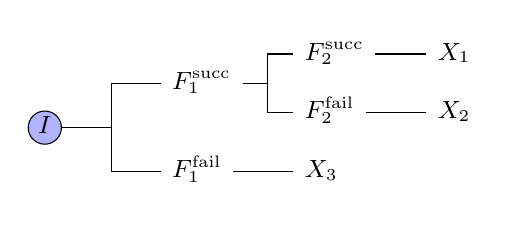
\begin{tikzpicture}
\tikzset{grow'=right,level distance=48pt}
\tikzset{execute at begin node=\strut}
\tikzset{every tree node/.style={anchor=base west}}
\tikzset{
    edge from parent/.append style={very thick},
    edge from parent/.style={
        draw,
        edge from parent path={
            (\tikzparentnode.east) -| ($(\tikzparentnode.east)!0.5!(\tikzchildnode.west)$) |- (\tikzchildnode.west)
        },
    },
    every node/.style={anchor=center,font=\small\bfseries, text centered, inner sep=0pt},
    every level 0 node/.style={circle, font=\small\bfseries, draw, fill=blue!30, inner sep=0pt},
    every internal node/.style={font=\small, inner sep=4pt},
    every leaf node/.style={rectangle, draw, fill=blue!30, minimum width=2.5cm, text centered},
    frontier/.style={distance from root=400pt},
}
\Tree [.\(I\)
    [.\(F_1^{\text{succ}}\)
        [.\(F_2^{\text{succ}}\)
            [.\(X_1\) ]
        ]
        [.\(F_2^{\text{fail}}\)
            [.\(X_2\) ]
        ]
    ]
    [.\(F_1^{\text{fail}}\)
        [.\(X_3\) ]
    ]
]
\end{tikzpicture}
\caption{Illustrative event tree with an initiating event \(I\), two functional events \(F_1\) and \(F_2\), and three end-states \(X_1, X_2, X_3\).}
\label{fig:event_tree_example}
\end{figure}
\begin{itemize}
  \item An Event Tree represents how an initiating event \(I\) can branch into multiple functional-event outcomes.
  \item Each functional event \(F_k\) may succeed or fail, driving the path toward a distinct end-state \(X_j\).  
  \item If \(\omega_j\) denotes one branch leading to \(X_j\), then the branch probability often factors as 
    \[
      p(\omega_j) \;=\; p(I)\;\times\;\prod_{k=1}^{n} \; p\bigl(F_k^{\alpha_k} \;\mid\; \text{all previous outcomes}\bigr).
    \]
  \item As a logical expression, each \(\omega_j\) translates to an AND of success/failure literals, and the overall set of end-states is an OR of these branches:
    \[
      \Omega \;=\;\omega_1 \;\lor\;\omega_2 \;\lor\;\dots\;\lor\;\omega_m.
    \]
  \item Consequently, ETs are in \emph{sum of products} (SOP) or \emph{disjunctive normal form} (DNF), where each product term identifies one success/failure path and the scenario-level outcome is the logical OR across all such paths.
  \vspace{4pt}
  \item Graphically straightforward, but can combinatorially expand for deep branching.
\end{itemize}
\end{frame}

\begin{frame}[t, allowframebreaks]
\frametitle{Fault Trees}
    \begin{figure}[h]
    \centering
    \includegraphics[width=0.5\textwidth]{1_concepts/ft.png}
    \caption{Fault tree with 6 basic events, top event $X = (a_1\bigwedge b_1) \bigvee (a_2\bigwedge b_2) \bigvee (a_3\bigwedge b_3)$}
    \label{fig:ft}
\end{figure}
\begin{itemize}
  \item A Fault Tree describes how a top event (system failure) can result from lower-level component or subsystem failures.
  \item Internal gates (AND, OR, \(k\)-of-\(n\), etc.) combine events in logical fashion:
    \[
      \text{Output} \;=\;
      \begin{cases}
         \bigwedge_{i=1}^k e_i, & \text{(AND)}\\
         \bigvee_{i=1}^k e_i, & \text{(OR)}\\
         \dots
      \end{cases}
    \]
  \item Basic events (BEs) in the leaves have assigned probabilities \(p(b)\).  Independence often assumed unless modeling common-cause failures.
  \item The top event failure probability can be written as:
    \begin{equation}
    \label{eq:top_event_probability_slides}
    \Pr[\text{Top Fail}] \;=\; \sum_{S \subseteq \,\mathcal{B}} 
      \Bigl[
        \pi_{F}(S, \text{Top}) 
        \prod_{b\in S} p(b)\prod_{b\notin S}[1 - p(b)]
      \Bigr].
    \end{equation}
\end{itemize}
\end{frame}

\begin{frame}[t, allowframebreaks]
\frametitle{Linking Event Trees and Fault Trees in PRA}
\begin{itemize}
  \item Real systems often combine:
    \begin{itemize}
      \item Forward branching dynamics via Event Trees (ET).
      \item Subsystem or component reliability logic via Fault Trees (FT).
    \end{itemize}
  \item An event tree branch may call a specific FT top event to collect system failure or success.
  \item Conversely, a fault tree output may feed back into an event tree branch as an initiating event or functional node outcome.
  \item This multi-level interconnection \(\implies\) a need for a unified model capturing both forward branching (ET) and hierarchical failure logic (FT).
\end{itemize}
\end{frame}

\begin{frame}[t, allowframebreaks]
\frametitle{Probabilistic Directed Acyclic Graph (PDAG)}
\begin{itemize}
  \item A PDAG is a Directed Acyclic Graph whose edges carry either:
    \begin{itemize}
      \item Conditional probabilities (e.g., for event tree branches).  
      \item Logical dependencies (e.g., for fault tree gates).
    \end{itemize}
  \item Nodes may include:
    \begin{itemize}
      \item Basic events (BEs) with known probabilities.
      \item ET or FT intermediate events storing partial results.
      \item Any top-level node (e.g., a final end-state) with no children.
    \end{itemize}
  \item The absence of cycles guarantees consistent flow from initial seeds (basic events, initiating events) to final outcomes.
  \item PDAG forms the structural backbone for bridging scenario-based expansions with gate-based logic in a single coherent representation.
\end{itemize}
\end{frame}

\subsection{Probabilistic Circuits Overview}
\begin{frame}[t, allowframebreaks]
\frametitle{Probabilistic Circuits: A Brief Overview}
    \begin{figure}[h]
    \centering
    \includegraphics[height=0.5\textheight]{1_concepts/pc.png}
    \caption{Probabilistic circuit with 4 inputs $X_i$, product gates (blue), sum gate (orange)}
    \label{fig:pc}
\end{figure}
\end{frame}

\begin{frame}[t, allowframebreaks]
\begin{itemize}
  \item A \textbf{probabilistic circuit} is a directed acyclic graph (DAG) that encodes a joint probability distribution through \emph{sum-gates} and \emph{product-gates}.
  \item \textbf{Sum-gates} approximate mixture distributions:
    \[
      p_v(\mathbf{x})
      \;=\;
      \sum_{u\in \operatorname{ch}(v)} \theta_{v,u}\,p_u(\mathbf{x}),
      \quad
      \text{with }
      \sum_{u\in \operatorname{ch}(v)} \theta_{v,u} = 1.
    \]
    Each child distribution is weighted by a nonnegative parameter \(\theta_{v,u}\).
  \item \textbf{Product-gates} factorize independent variable sets:
    \[
      p_v(\mathbf{x})
      \;=\;
      \prod_{u\in \operatorname{ch}(v)} p_u\bigl(\mathbf{x}_{u}\bigr),
    \]
    assuming disjoint subsets of variables for each child \(u\).
  \item \textbf{Leaf nodes} (inputs) often correspond to known base distributions. When evaluated upward through the DAG, each internal node yields its own distribution, culminating in a root node that represents the full model.
  \item \textbf{Key motivation}:
    \begin{itemize}
      \item Tractable inference: evaluation and certain marginal or conditional queries can be performed in time proportional to circuit size.  
      \item Decomposability and modularity: separate, interpretable substructures that can be reused or combined for large-scale systems.
    \end{itemize}
\end{itemize}
\end{frame}

\subsection{PRA PDAGs to Probabilistic Circuits}
\begin{frame}[allowframebreaks]
\frametitle{Compiled PRA Graphs are PDAGs}
\begin{itemize}
  \item A unified PRA model can be viewed as
    \[
      \mathcal{M} 
      \;=\;
      \langle 
        \mathcal{V},\,\mathcal{A},\, \{p(b)\},\, \{\theta_{u\to v}\},\,\pi_{F}
      \rangle,
    \]
    where \(\mathcal{V}\) includes basic events, ET nodes, and FT gates, and \(\mathcal{A}\) is the acyclic edge set.
  \item Event-tree edges carry transitional probabilities \(\theta_{u\to v}\) summing to 1 from each node.
  \item Fault-tree nodes embed Boolean logic \(\pi_F\) that checks if inputs fail under a subset of basic events.
  \framebreak
  \item This PDAG perspective:
    \begin{itemize}
      \item Ensures systematic accounting of all scenario paths and subsystem logic.
      \item Aligns naturally with tractable Probabilistic Circuits, since each node’s distribution/function can be embedded in a sum-product style DAG.
      \item Offers a foundation for efficient Monte Carlo or advanced inference methods.
    \end{itemize}
    \vspace{6pt}
    \item Ongoing work to bridge PRA PDAG semantics with Probabilistic Circuits:
    \begin{itemize}
      \item PDAGs can be transformed to equivalent canonical forms (there are tradeoffs).
    \end{itemize}
\end{itemize}
\end{frame}
\section{Research Objective 2: Develop data-parallel methods for evaluating Boolean circuits}
\begin{frame}
    \Large{\centerline{\textbf{Research Objective 2}}}
    \vspace{6pt}
    \large{\centerline{\textbf{Develop data-parallel methods for evaluating Boolean circuits}}}
\end{frame}

%% ------------------------------------------------------------------
%% From Truth Table to Bit-Parallelism
%% ------------------------------------------------------------------
\subsection{Bitwise Kernels}
\begin{frame}{Boolean Truth Table – Single Bit}
\centering
\begin{tabular}{c|c|c|c|c|c|c|c}
$X$ & $Y$ & AND & OR & XOR & NAND & NOR & XNOR \\ \hline
0 & 0 & 0 & 0 & 0 & 1 & 1 & 1 \\
0 & 1 & 0 & 1 & 1 & 1 & 0 & 0 \\
1 & 0 & 0 & 1 & 1 & 1 & 0 & 0 \\
1 & 1 & 1 & 1 & 0 & 0 & 0 & 1 \\
\end{tabular}
\vspace{8pt}
\begin{itemize}
  \item Classical gate evaluation operates \emph{bit-by-bit}.  Throughput $\propto$ number of Boolean operations.
  \item Perform \textbf{64} of these truth-table lookups in one machine instruction.
\end{itemize}
\end{frame}

%% ------------------------------------------------------------------
%% Eight Bits in Parallel
%% ------------------------------------------------------------------
\begin{frame}{Extending to a 64-Bit Word}
\begin{columns}
  \column{0.55\textwidth}
    \begin{itemize}
      \item Pack 64 independent Bernoulli trials into one byte.
      \item Bitwise primitives act \emph{independently} on every bit position.
      \item Hardware native instructions guarantee ns latency.
    \end{itemize}
  \column{0.45\textwidth}
    \centering
    \includegraphics[height=0.7\textheight]{2_framework/research_objective_2_sycl_eval/bitwise_xy_inv.png}
\end{columns}
\end{frame}


% special case for k/n kernels
\begin{frame}[t]{Handling Voter Logic - Expansion} 
  \begin{columns}
    \column{0.60\textwidth}
    {
      \textbf{The Simplest Type of Query: Eval(G)}\par
      \begin{itemize}
          \item {Set the inputs [on/off].}
          \item {Observe the outputs [on/off].}
      \end{itemize}\par
      \vspace{2pt}
      \tiny{\textbf{\emph{{Can be used as a building block for an embedding ML model.}}}}\par
            \vspace{10pt}
      \normalsize\textbf{But how to handle K/N gates?}

    }
     \column{0.4\textwidth}
      \input{1_concepts/ft_3_of_5}\par % Replace with your image file
  \end{columns}
\end{frame}


%% ------------------------------------------------------------------
%% SYCL Execution Model
%% ------------------------------------------------------------------
\subsection{The SYCL Execution Model}
\begin{frame}{SYCL Execution Model in a Nutshell}
      \centering
      \includegraphics[width=0.9\textwidth]{2_framework/research_objective_2_sycl_eval/sycl.png}\par % Replace with your image file
\end{frame}

%% ------------------------------------------------------------------
%% SYCL Execution Model
%% -----------------------------------------------------------------

\begin{frame}{SYCL Execution Model in a Nutshell}
  \begin{columns}
    \column{0.3\textwidth}
      \tiny
      \begin{description}
        \item[Host] submits \texttt{queue.submit()} with a \texttt{kernel\_name}.
        \item[ND-Range] $\langle\,\text{global}\;3\!\times\!\text{local}\,\rangle$ defines grid.
        \item[Work-Group] maps to CUDA block / OpenCL work-group.
        \item[Sub-Group] (warp/wavefront) gives warp-level shuffle & ballot ops.
        \item[Device USM] used for persistent bit-packed buffers.
      \end{description}
    \column{0.7\textwidth}
      \centering
      \includegraphics[width=1\textwidth]{2_framework/research_objective_2_sycl_eval/sycl.png}\par % Replace with your image file
  \end{columns}
\end{frame}

%% ------------------------------------------------------------------
%% Mapping PDAG Layers to Kernels
%% ------------------------------------------------------------------
\subsection{Kernel Execution}
\begin{frame}{Mapping PDAG Layers to SYCL Kernels}
    \tiny
  \begin{enumerate}
    \item Topological sort $\Rightarrow$ depth index $d$.
    \item All nodes with depth $d$ share \emph{identical fan-in length}.  \texttt{range<3>} := $(\text{batch},\text{gate},\text{bitpack})$.
    \item One kernel per layer; gate type dispatched via template specialization.
    \item Streams results to next-depth buffer in global memory.
  \end{enumerate}
  \vspace{-42pt}
  \begin{columns}
      \column{0.6\textwidth}
        \centering
      \includegraphics[width=1\textwidth]{2_framework/research_objective_2_sycl_eval/sycl.png}
      \column{0.4\textwidth}
        \centering
        \includesvg[height=0.9\textheight]{1_concepts/dag_pass_2.svg}
  \end{columns}

\end{frame}

\begin{frame}{Eval Query Performance on Generic Backends}
\centering
        \includegraphics[height=0.9\textheight]{2_framework/research_objective_2_sycl_eval/slides_nodes_vs_throughput.eps}
\end{frame}

\begin{figure}[hb]
    \centering
    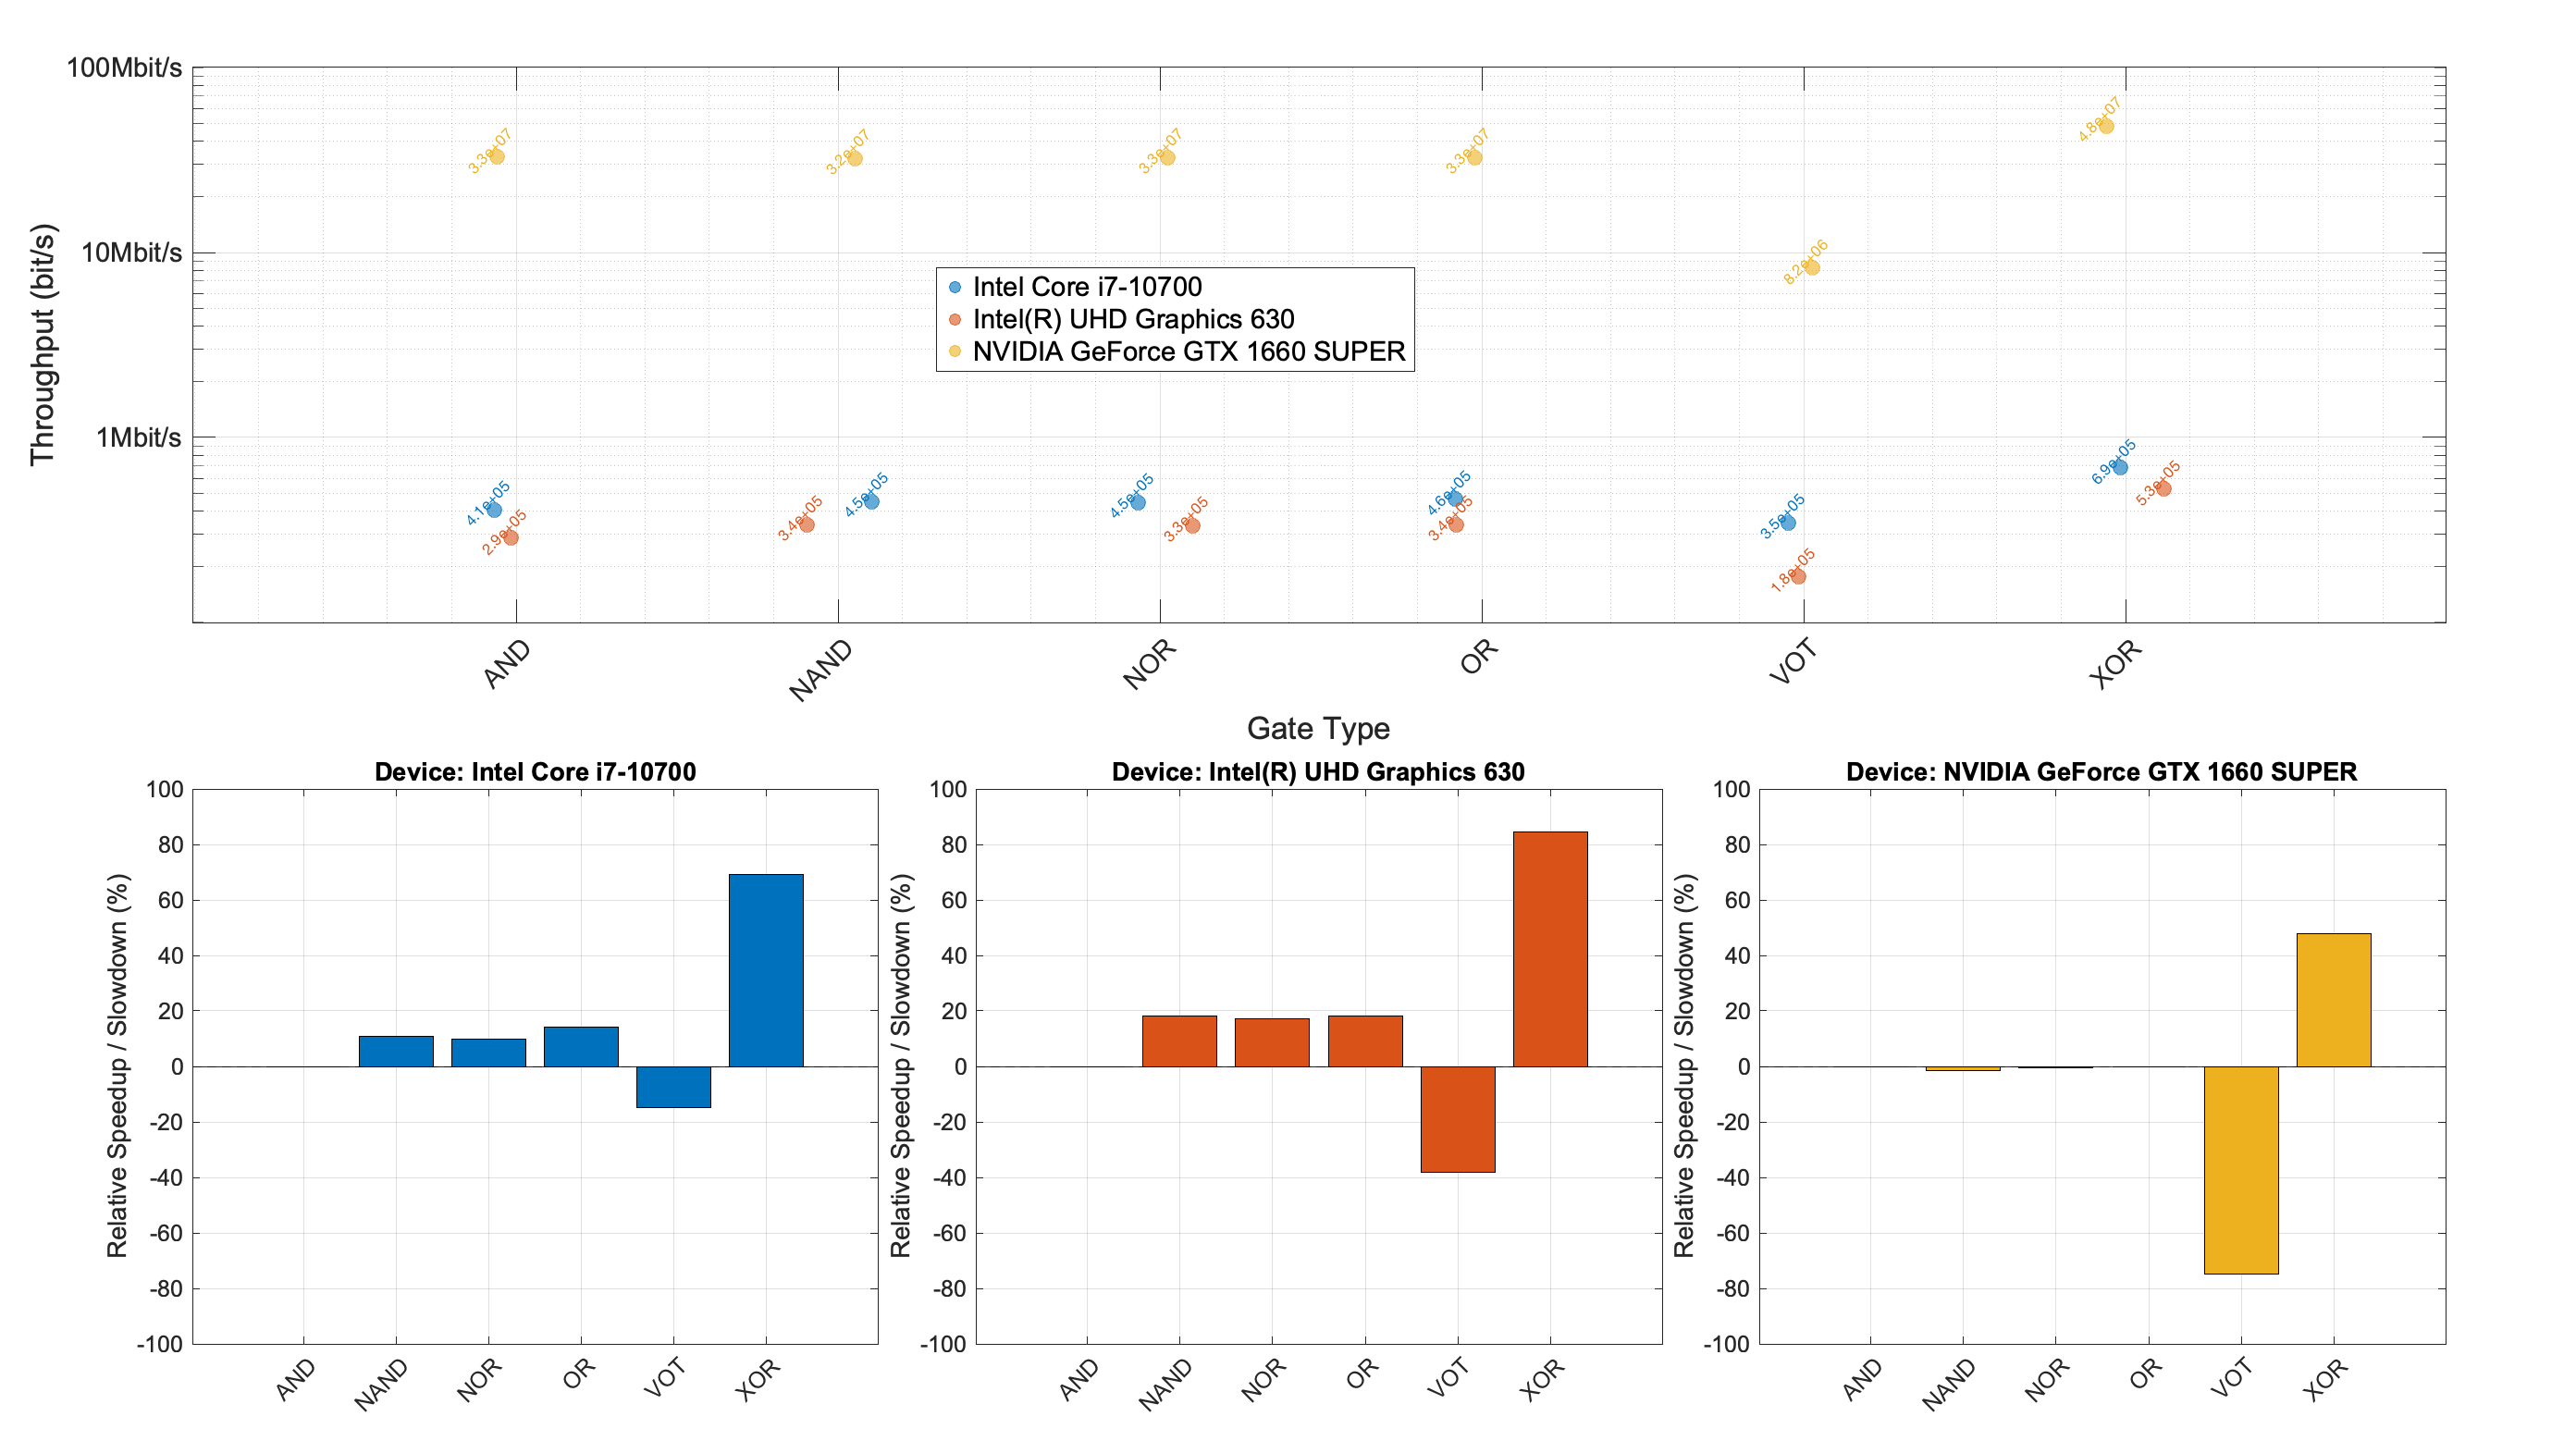
\includegraphics[height=0.8\textheight]{execution_model/slides_throughput_by_gate_type.eps}
    \caption{(Top) Throughput in bit/second on various backends for different gate types. (Bottom) \% Relative speedup/slowdown as compared to the AND gate.}
    \label{fig:gate_throughput}
\end{figure}

%% throughput graph
\begin{frame}{Eval Query Performance on Discrete GPUs}
  \begin{columns}
    \column{0.60\textwidth}
    {
      \begin{itemize}
          \item {Latency: 20-30 $ms$ per layer.}
          \item {Throughput: Graph depth and VRAM bound (see plot).}
          \item {Benchmarked on Nvidia GTX 1660 [6GB].}
          \item {Graph sizes: from $\approx 50$ to $\approx 2000$ nodes.}
          \item {Evals: from 16M to 1B per node per pass.}
      \end{itemize}
      \vspace{10pt}
      \textbf{Q: Are these enough samples to estimate the Expectation Query?}
    }
     \column{0.4\textwidth}
        \centering
        \includesvg[height=0.9\textheight]{1_concepts/mem_allocation_lines_zoom.svg}
  \end{columns}
\end{frame}





% ============================================================================
%  Research Objective 3 — Monte-Carlo Probability Estimation
%  Replaces prior preliminary version; integrates new pipeline & diagnostics
% ============================================================================
\section{Research Objective 3: Develop data-parallel Monte Carlo algorithms for probability estimation}

% ----------------------------------------------------------------------------
%  Title Frame
% ----------------------------------------------------------------------------
\begin{frame}
  \Large\centering\textbf{Research Objective 3}\\[6pt]
  \large Develop data-parallel Monte-Carlo methods for estimating probabilities on unified PDAGs
\end{frame}

% ----------------------------------------------------------------------------
%  Bridge: From Boolean Evaluation to Probabilistic Inference
% ----------------------------------------------------------------------------
\begin{frame}{Bridging Boolean Evaluation and Probabilistic Inference}
  \begin{itemize}
    \item Previous objective delivered \emph{bit-parallel gate kernels} that evaluate a PDAG layer in $\mathcal{O}(1)$ machine words.
    \item To quantify \alert{risk}, we must attach \emph{probability distributions} to the PDAG leaves and propagate forward.
    \item Strategy: embed a Monte-Carlo engine that
          \begin{enumerate}
            \item draws bit-packed Bernoulli samples for \textbf{all} basic events, and
            \item reuses the same gate kernels to evaluate each random draw.
          \end{enumerate}
    \item One kernel pipeline therefore suffices for \textbf{both} deterministic logic and stochastic sampling.
  \end{itemize}
\end{frame}

\subsection{Back to Working Example: One Initiating Event, Three Fault Trees, Six Basic Events, Five End States}
\begin{frame}
  \begin{columns}
    \column{0.66\textwidth}
      \includesvg[height=\textheight]{1_concepts/dag_pass_3.svg} % Replace with your image file
     \column{0.33\textwidth}
      \includesvg[width=\linewidth]{1_concepts/pra-model.svg} % Replace with your image file
  \end{columns}  
\end{frame}

% ----------------------------------------------------------------------------
%  End-to-End Sampling Pipeline
% ----------------------------------------------------------------------------
\begin{frame}{End-to-End Sampling Pipeline (one iteration)}
  \begin{columns}
    \column{0.6\textwidth}
      \includesvg[height=0.9\textheight]{1_concepts/dag_pass_3.svg} % Replace with your image file
     \column{0.4\textwidth}
  \tiny   
  \begin{enumerate}[<+->]
    \item \textbf{Basic-Event Kernel:} generate random draws.
    \item \textbf{Gate Kernels:} evaluate PDAG layers using hardware-native logic primitives.
    \item \textbf{Tally Kernel:} count number of ones, update counters, compute estimates.
  \end{enumerate}
  \end{columns}  
\end{frame}

% ----------------------------------------------------------------------------
%  Monte-Carlo Algorithm Recap (keeps most of prior text)
% ----------------------------------------------------------------------------
\subsection{MC Sampling Theory}

\begin{frame}{Monte-Carlo Sampling over PDAGs}
  \small
  \begin{enumerate}
    \item Draw $\mathbf{x}^{(i)}\sim\prod_{b\in\mathcal{B}}\text{Bernoulli}\bigl(p_b\bigr)$ in \textbf{bit-packed} form.
    \item Evaluate the Boolean function $F\colon\{0,1\}^{|\mathcal{B}|}\!\to\!\{0,1\}$ (root node) using the gate kernels.
    \item Record $Y^{(i)} \!=\! F\bigl(\mathbf{x}^{(i)}\bigr)$ \;(failure indicator).
  \end{enumerate}
  After $N$ iterations
  \[\widehat{P}_N = \frac1N\sum_{i=1}^N Y^{(i)},\qquad \operatorname{SE}(\widehat P_N)=\sqrt{\frac{\widehat P_N(1-\widehat P_N)}{N}}.\]
  Error shrinks as $\mathcal{O}\!\bigl(N^{-1/2}\bigr)$; variance-reduction extensions discussed shortly.
\end{frame}


% ----------------------------------------------------------------------------
%  Basic-Event Sampling Kernel
% ----------------------------------------------------------------------------
\begin{frame}{Basic-Event Sampling Kernel}
\begin{columns}
  \column{0.7\textwidth}
  \footnotesize
  \begin{itemize}
    \item Each basic event $b\in\mathcal{B}$ is modelled as an independent \textbf{Bernoulli} random variable $X_b\sim\operatorname{Bernoulli}(p_b)$.
    \item A single Monte--Carlo iteration packs $\omega = 8\,\mathrm{sizeof}(\texttt{bitpack\_t}) = 64$ independent trials into one machine word.
    \item For batch index $b$, bit--pack $p$, lane $\lambda$:
          $\displaystyle X_{b,p,\lambda}\sim\operatorname{Bernoulli}(p_b)$.
    \item The basic--event kernel uses the counter--based \textsc{Philox--4×32--10} PRNG; counters are derived from $(b,p,\lambda,t)$, guaranteeing reproducibility and inter--thread independence.
    \item After one iteration ($N = B P \omega$ trials) the sufficient statistics per basic event are
          $\displaystyle s_b = \sum_{p,\lambda} X_{b,p,\lambda}$,\;
          $\widehat p_b = s_b/N$,\;
          $\operatorname{SE}(\widehat p_b)=\sqrt{\widehat p_b(1-\widehat p_b)/N}$.
  \end{itemize}
       \column{0.3\textwidth}
       \includesvg[width=\textwidth]{2_framework/research_objective_3_mc_sampling/sample_event_A.svg}\par
  \end{columns}
\end{frame}


%% needs a frame on tallies, with estimator statistics, convergence properties
% ----------------------------------------------------------------------------
%  Tally Kernel & Estimator Convergence
% ----------------------------------------------------------------------------
\begin{frame}{Tally Kernel}
  \footnotesize
  \begin{itemize}
    \item For a designated node $v$ (e.g. system top event) define $Y_{p,\lambda}^{(t)} = F_v\bigl(\mathbf{X}_{\cdot,p,\lambda}^{(t)}\bigr)\in\{0,1\}$.
    \item \textbf{Tally kernel} executes a single SIMD \texttt{popcount} per bit-pack to obtain the per-iteration count
      $\displaystyle s_v^{(t)} = \sum_{p,\lambda} Y_{p,\lambda}^{(t)}$.
    \item Cumulative statistics after $T$ iterations ($N_T = T N$ trials):
      \[ S_v = \sum_{t=1}^{T} s_v^{(t)},\qquad \widehat P_v = \frac{S_v}{N_T}. \]
    \item Unbiased variance estimator
      \[ \widehat{\sigma}^2_v = \frac{\widehat P_v\bigl(1-\widehat P_v\bigr)}{N_T}. \]
    \item \textbf{Central Limit Theorem.}  As $T\to\infty$
      \[ \frac{\widehat P_v - P_v}{\widehat \sigma_v}\;\xrightarrow{\,\mathcal{D}\,}\;\mathcal N(0,1). \]
  \end{itemize}
\end{frame}

%% run with runaway iterations.
%% show a run with too many iterations, and make the case for developing a robust convergence criteria.
% ----------------------------------------------------------------------------
%  The Cost of Runaway Iterations (Motivation)
% ----------------------------------------------------------------------------
\begin{frame}{When "More Samples" is Wasteful}
  \begin{columns}
    \column{0.35\textwidth}
      \footnotesize
      \begin{itemize}
        \item Fixed iteration budgets ($N$ large and hard-wired) risk \emph{massive}\, oversampling when $P_v$ is moderate (\(\approx10^{-4}\)–\(10^{-1}\)).
      \end{itemize}
    \column{0.65\textwidth}
      \centering
      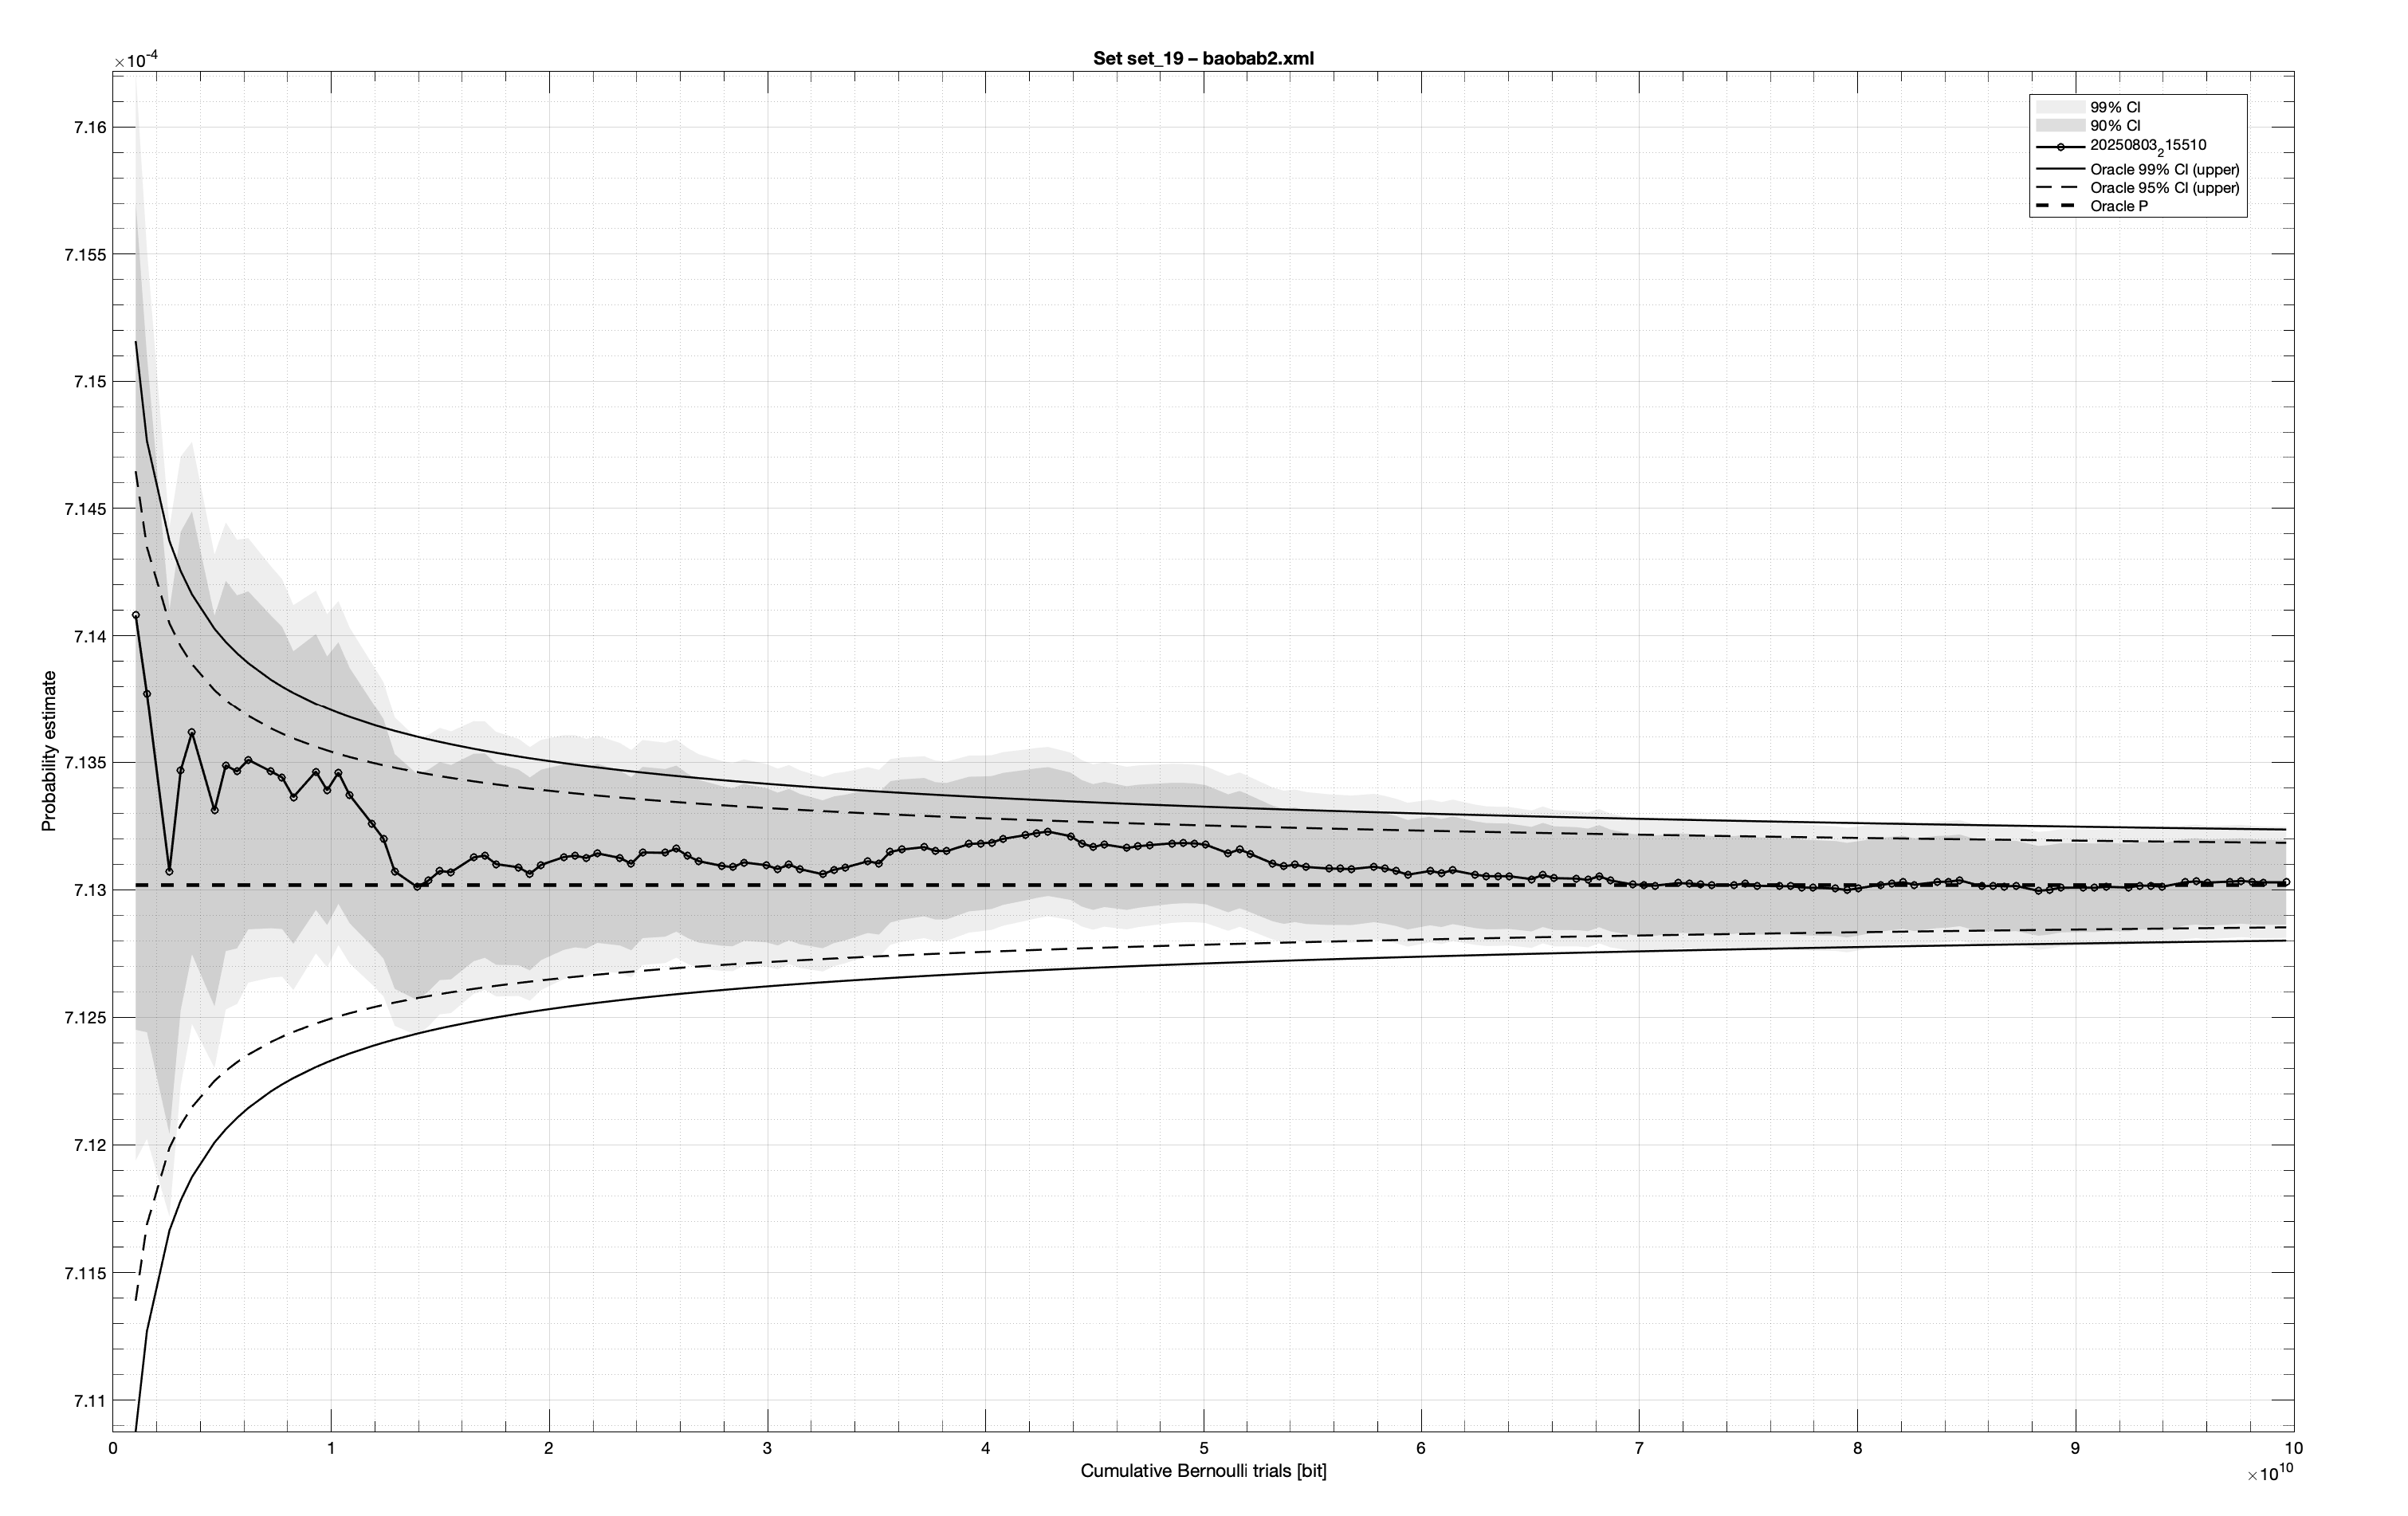
\includegraphics[width=0.95\linewidth]{2_framework/research_objective_3_mc_sampling/conv_fig_02.eps} % create trace: half-width vs iterations
      \vspace{-6pt}
  \end{columns}
\end{frame}


\section{Research Objective 4: Convergence Guarantees}
\begin{frame}
    \Large{\centerline{\textbf{Research Objective 4}}}
    \vspace{6pt}
    \large{\centerline{\textbf{Develop Robust Convergence Criteria}}}
\end{frame}
\subsection{Interpretation of Probability}
% ------------------------------------
%  Criterion 1 – Frequentist Half-Width
% ------------------------------------
\begin{frame}{Criterion 1: Frequentist Half-Width (Wald)}
  \footnotesize
  Let $\{Y^{(i)}\}_{i=1}^N$ be i.i.d. Bernoulli trials with $P=\Pr[Y=1]$.  The estimator $\widehat P_N=\tfrac1N\sum_i Y^{(i)}$ obeys the CLT:
  \[\sqrt{N}\,\bigl(\widehat P_N-P\bigr) \;\xrightarrow{d}\; \mathcal N\bigl(0, P(1-P)\bigr).\]
  A $(1-\alpha)$ two–sided \textbf{Wald} interval is therefore
  \[ \widehat P_N \;\pm\; z_{1-\alpha/2}\, \sqrt{\tfrac{\widehat P_N(1-\widehat P_N)}{N}}. \]
  \begin{alertblock}{Stopping rule}
   \textbf{Half-width:} $h_N^{\text{lin}}(z)=z\sqrt{\widehat P_N(1-\widehat P_N)/N}.$ Declare convergence when $h_N^{\text{lin}}/\widehat P_N\le \varepsilon_{\text{rel}}$.
  \end{alertblock}
  \begin{block}{Intuition}
    Shrinks a \emph{relative} confidence band around the estimate; fast for moderate $P$, slow for rare events where $\widehat P_N\ll10^{-4}$.
  \end{block}
\end{frame}

% ------------------------------------
%  Criterion 2 – Bayesian Credible Interval
% ------------------------------------
\begin{frame}{Criterion 2: Bayesian Credible Interval (Jeffreys prior)}
  \footnotesize
  Prior $p\sim\text{Beta}\bigl(\tfrac12,\tfrac12\bigr)$ is invariant under re-parameterization.  After $s$ successes and $f$ failures the posterior is
  \[ p\mid\text{data}\;\sim\; \text{Beta}\bigl(s+\tfrac12,\,f+\tfrac12\bigr). \]
  The central $(1-\alpha)$ credible interval $[q_t,q_{1-t}]$ with $t=\alpha/2$ has
  \begin{alertblock}{Stopping rule}
  \textbf{half-width} $h_N^{\text{Bayes}}=(q_{1-t}-q_t)/2$. Convergence when $h_N^{\text{Bayes}}/\widehat P_N\le \varepsilon_{\text{rel}}^{\text{Bayes}}$.
  \end{alertblock}
  \begin{block}{Intuition}
  Integrates parameter uncertainty; maintains correct coverage even when $\widehat P_N$ is based on only a handful of observed failures (rare-event tails).
  \end{block}
\end{frame}

% ------------------------------------
%  Criterion 3 – Information Gain
% ------------------------------------
\begin{frame}{Criterion 3: Information-Theoretic Gain}
  \small
  Posterior entropy of $\text{Beta}(\alpha,\beta)$ is
  \[ H(\alpha,\beta)=\ln B(\alpha,\beta)- (\alpha-1)\psi(\alpha)- (\beta-1)\psi(\beta)+ (\alpha+\beta-2)\psi(\alpha+\beta). \]
  After a batch $(\Delta s,\Delta f)$ the \textbf{information gain} is
  \[ I_{\text{batch}} = H(\alpha,\beta) - H(\alpha+\Delta s,\,\beta+\Delta f). \]
  \begin{alertblock}{Stopping rule}
   Stop when $I_{\text{batch}}<I_{\min}$ bits (default $10^{-4}$).
  \end{alertblock}
  \begin{block}{Intuition}
 Scale-free; halts when each new batch conveys negligible Shannon information, preventing oversampling when $P$ is either very small or very large.
  \end{block}
\end{frame}

% ----------------------------------------------------------------------------
%  Composite Convergence Diagnostics
% ----------------------------------------------------------------------------
\begin{frame}{Composite Convergence Diagnostics}
  \begin{columns}
    \column{0.55\textwidth}
      \begin{itemize}
        \item \textbf{Frequentist half-width} $h_v(z)$ on linear and log scale.
        \item \textbf{Bayesian credible interval} with Jeffreys prior.
        \item \textbf{Information gain} $I_{\text{batch}}<10^{-4}$ bits.
        \item Run stops when \emph{all} criteria satisfied for every monitored node.
            \item \textbf{Composite stopping rule.}  Convergence declared when
      \[
        \frac{z_{1-\alpha/2}\,\widehat \sigma_v}{\widehat P_v} \le \varepsilon_{\text{rel}},\quad
        h^{\log}_v(z) \le \varepsilon^{\log},\quad
        I_{\text{batch}} < 10^{-4}\;\text{bits}.
      \]
      \end{itemize}
    \column{0.45\textwidth}
      \includegraphics[width=\linewidth]{2_framework/research_objective_3_mc_sampling/ci_trace.pdf} % create a small diagnostic trace figure
  \end{columns}
\end{frame}




\section{Research Objective 5: Case Studies and Benchmarks}
\begin{frame}
    \Large{\centerline{\textbf{Research Objective 5}}}
    \vspace{6pt}
    \large{\centerline{\textbf{Case Studies and Benchmarks}}}
\end{frame}

\subsection{Aralia Fault Tree Data Set}
\begin{frame}[t]
\frametitle{Overview: Aralia Dataset}
\begin{itemize}
  \item \textbf{Dataset Composition:} The Aralia collection consists of 43 distinct fault trees, each with varying numbers of basic events (BEs), gate types (AND, OR, K/N, XOR), and minimal cut-set counts.  
  \item \textbf{Diverse Problem Sizes:} Small trees (e.g.\ 25--32 BEs) through large models with over 1{,}500 BEs.  
  \item \textbf{Wide Probability Range:} Top-event probabilities spanning from rare events near \(10^{-13}\) to fairly likely failures with probability above 0.7.  
  \item \textbf{Model Variability:} Some trees are primarily AND/OR, others incorporate more advanced gates (K/N, XOR, NOT), providing thorough coverage of typical (and atypical) fault tree logic structures.
\end{itemize}
\end{frame}

\begin{frame}[allowframebreaks]
    \input{4_casestudy/3_table_aralia_ft_dataset}
\end{frame}

\subsection{Benchmarking Procedure}
\begin{frame}[t]
\frametitle{Benchmarking Setup: Hardware and Environment}
\begin{itemize}
  \item \textbf{Target Hardware:}
    \begin{itemize}
      \item GPU: NVIDIA\textsuperscript{\textregistered} GeForce GTX 1660 SUPER (6\,GB GDDR6, 1{,}408 CUDA cores).
      \item CPU: Intel\textsuperscript{\textregistered} Core\textsuperscript{TM} i7-10700 (2.90\,GHz, turbo-boost, hyperthreading).
    \end{itemize}
  \item \textbf{Software Stack:}
    \begin{itemize}
      \item SYCL-based (AdaptiveCpp/HipSYCL), with LLVM-IR JIT for kernel compilation.
      \item Compiler optimization at \texttt{-O3} for efficient code generation.
      \item Repeated runs (5+) to mitigate transient variations.
    \end{itemize}
  \item \textbf{Measured Time:} Includes entire wall-clock duration, from host-device transfers and JIT compilation to final result collection.
\end{itemize}
\end{frame}

\subsection{Accuracy Benchmarks}
\begin{frame}
    \begin{figure}[h]
    \centering
    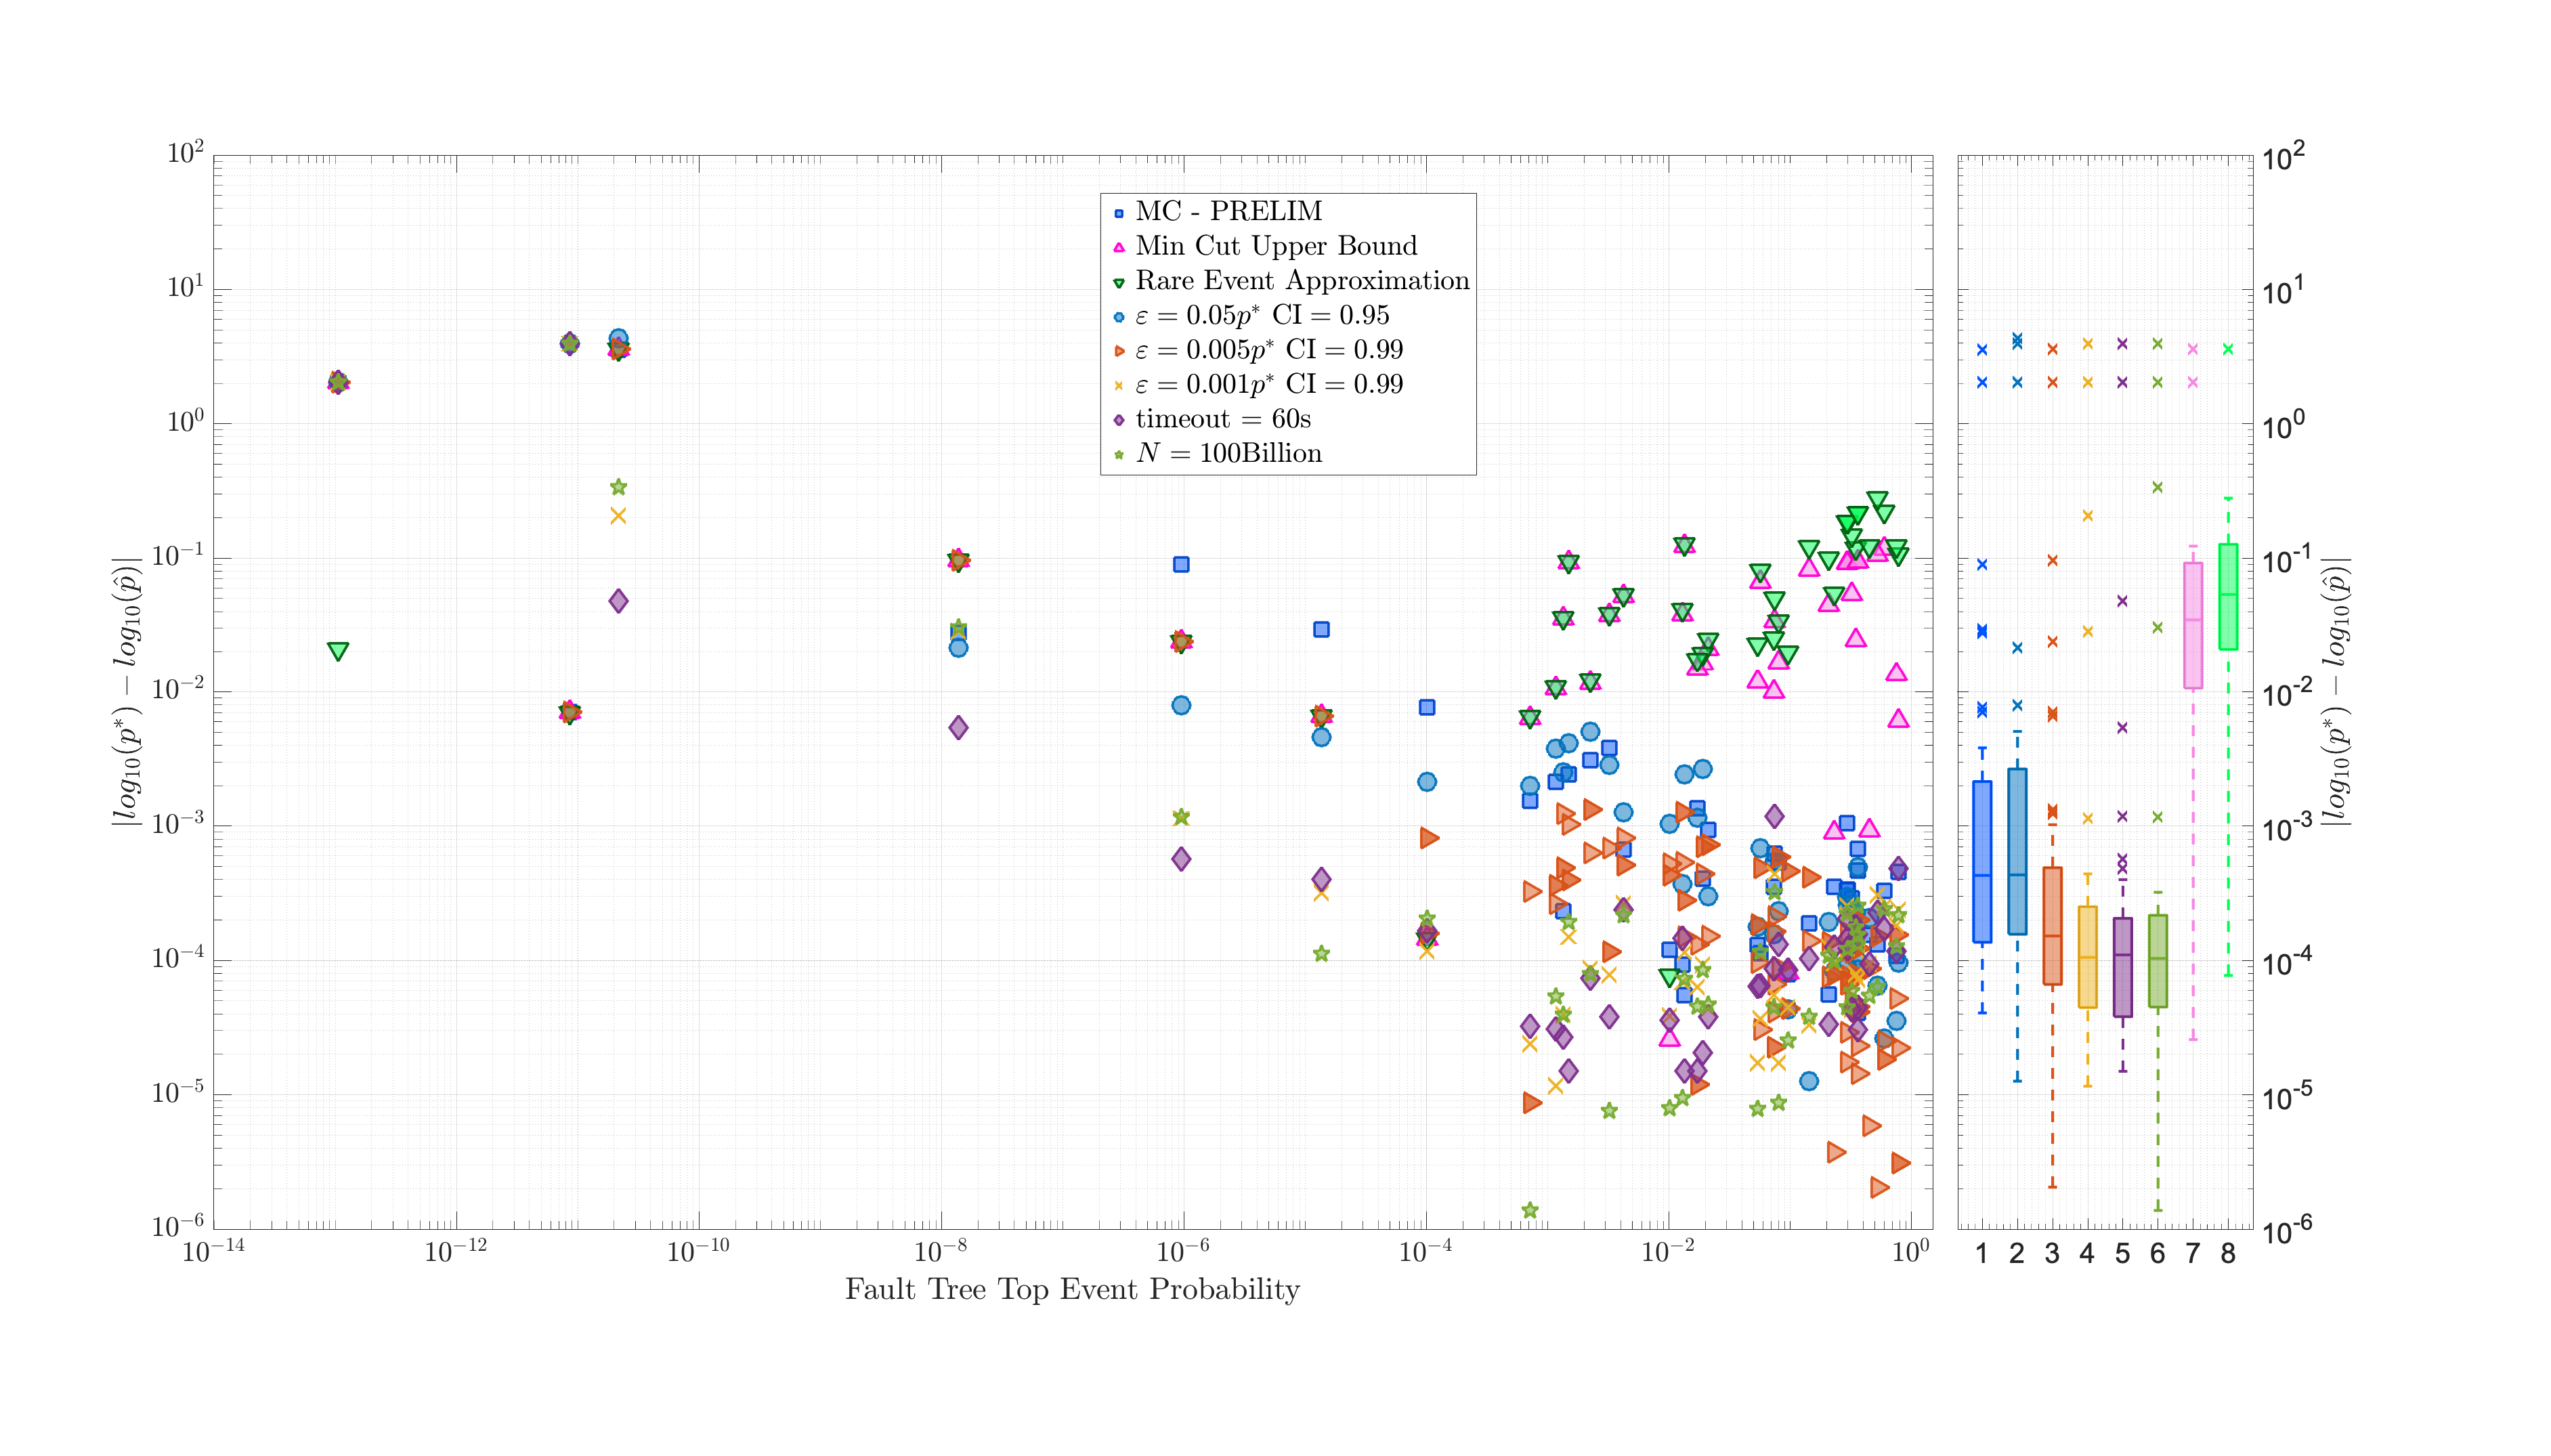
\includegraphics[height=1.1\textheight]{4_casestudy/abs_err.eps}
    \label{fig:mae_vs_logp}
\end{figure}
\end{frame}

\subsection{Accuracy vs. Time to Convergence}
\begin{frame}
\begin{figure}[p]
    \centering
    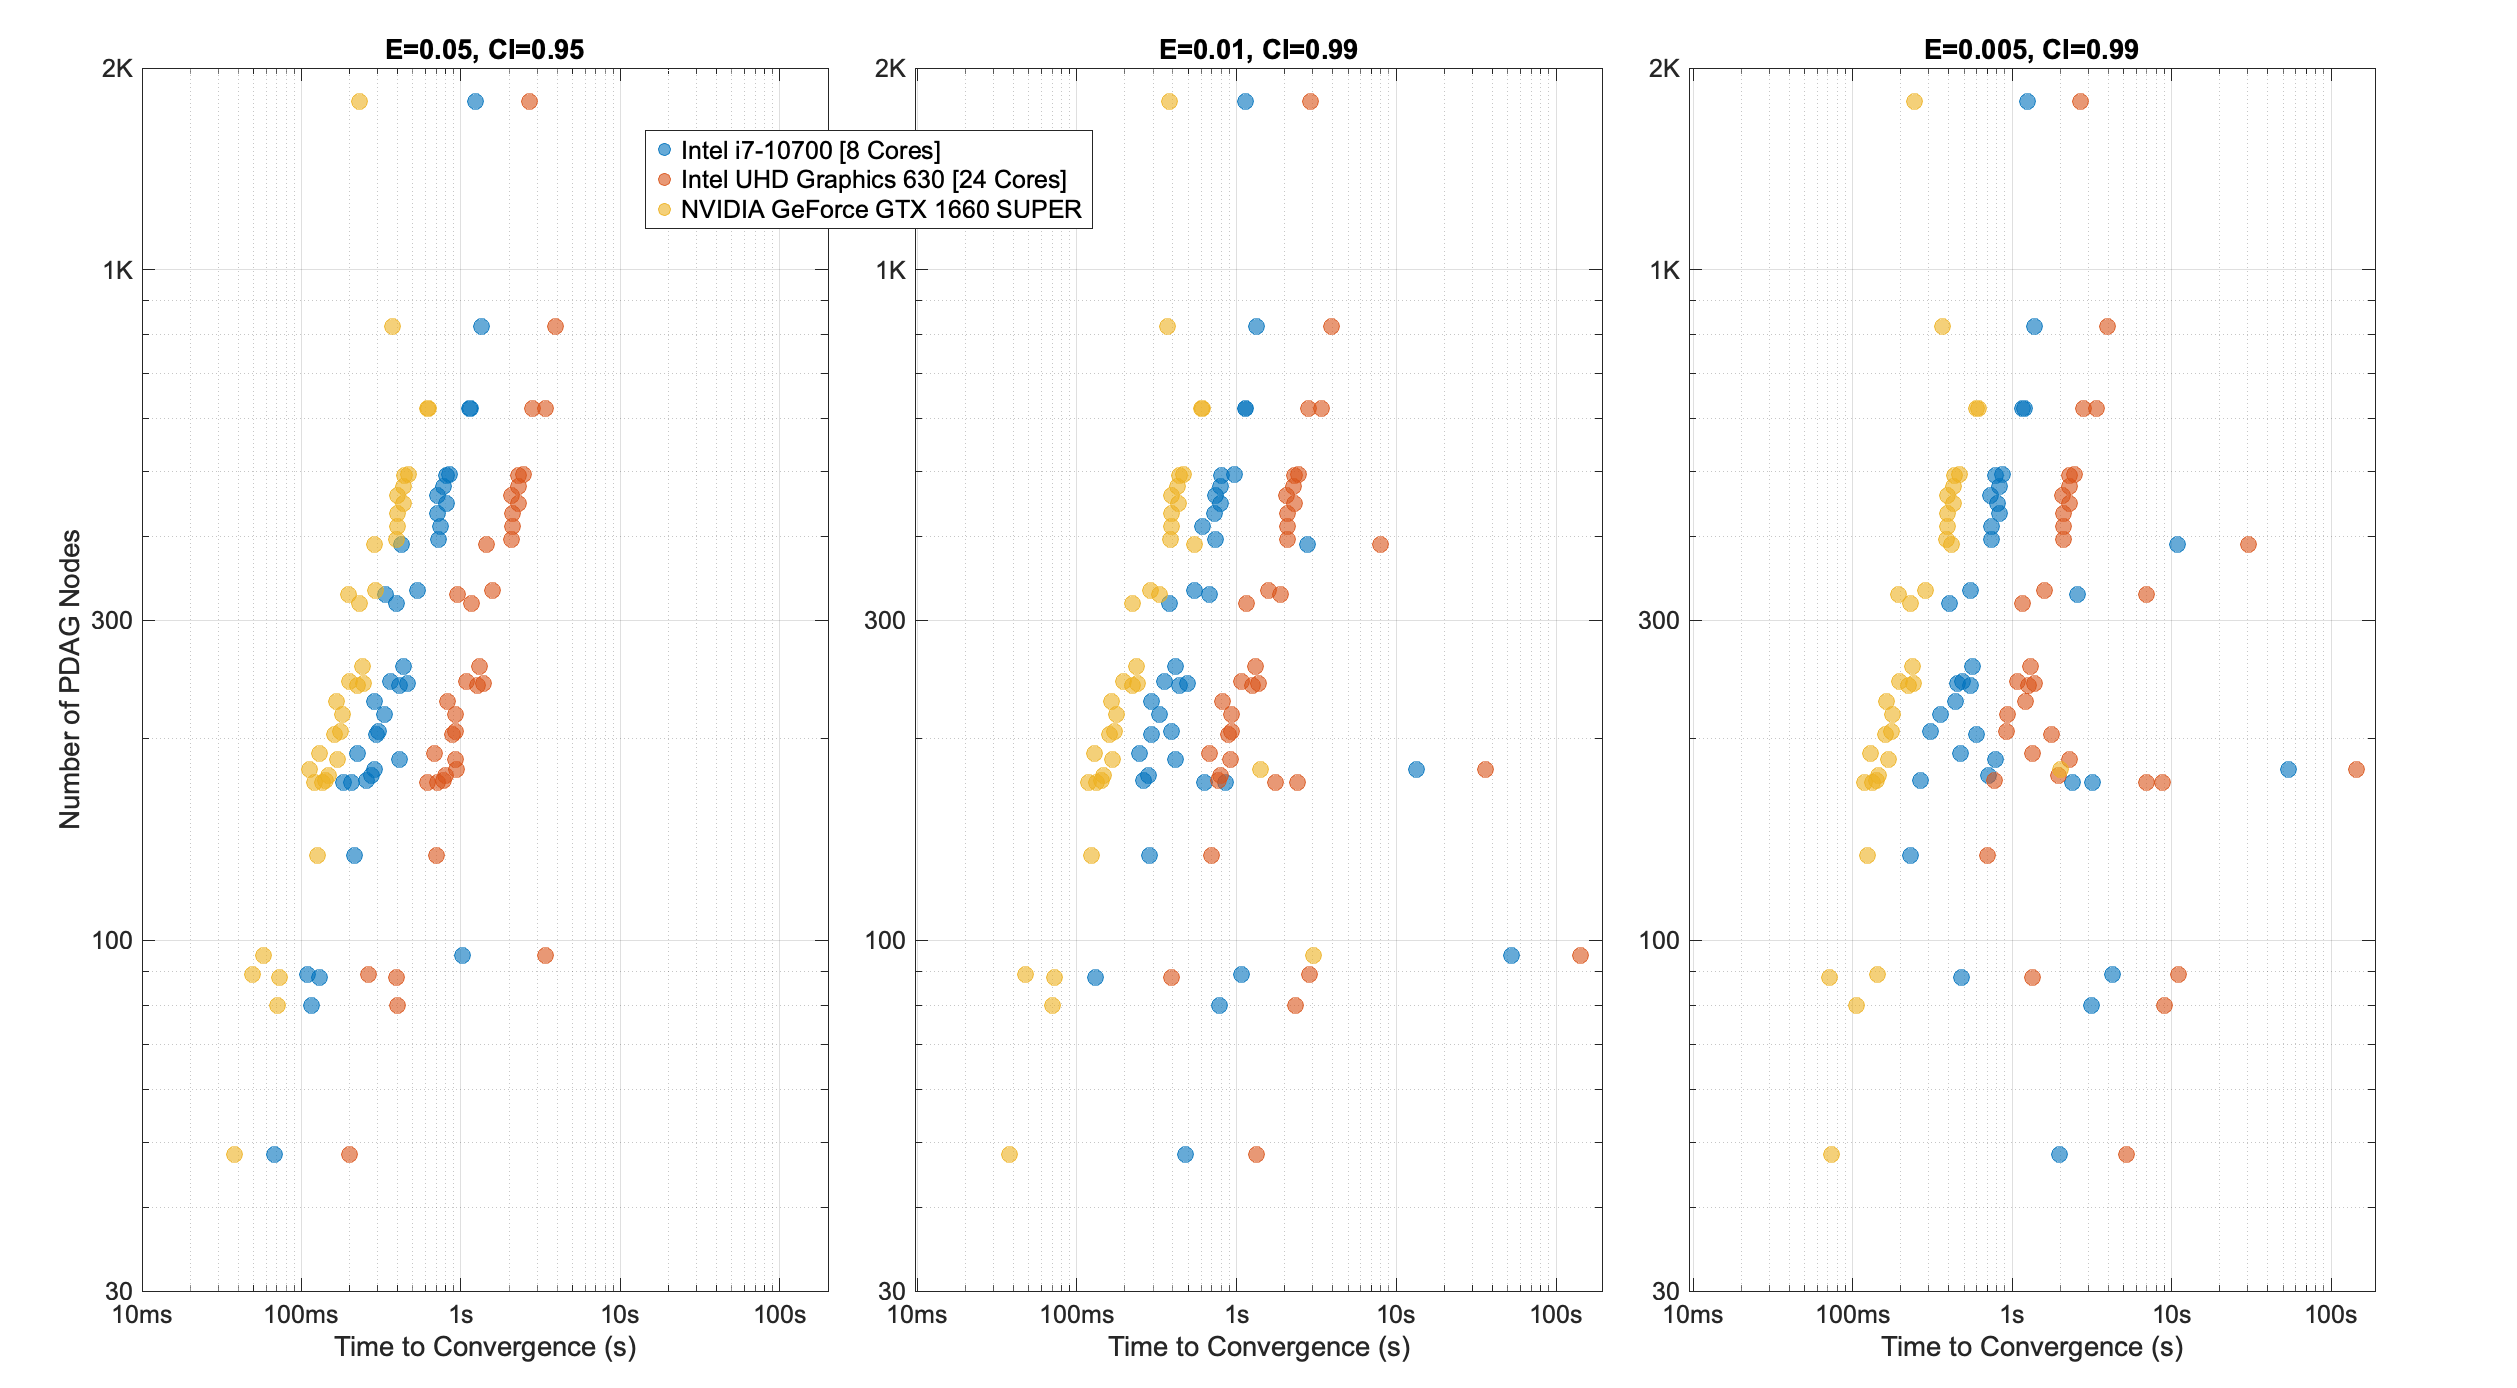
\includegraphics[height=1\textheight]{4_casestudy/throughput/slides_nodes_vs_convergence.eps}
    \caption{Time to convergence for different accuracy targets.}
    \label{fig:nodes_vs_convergence}
\end{figure}
\end{frame}

\subsection{Convergence Runs}
\begin{frame}
\begin{figure}[p]
    \centering
    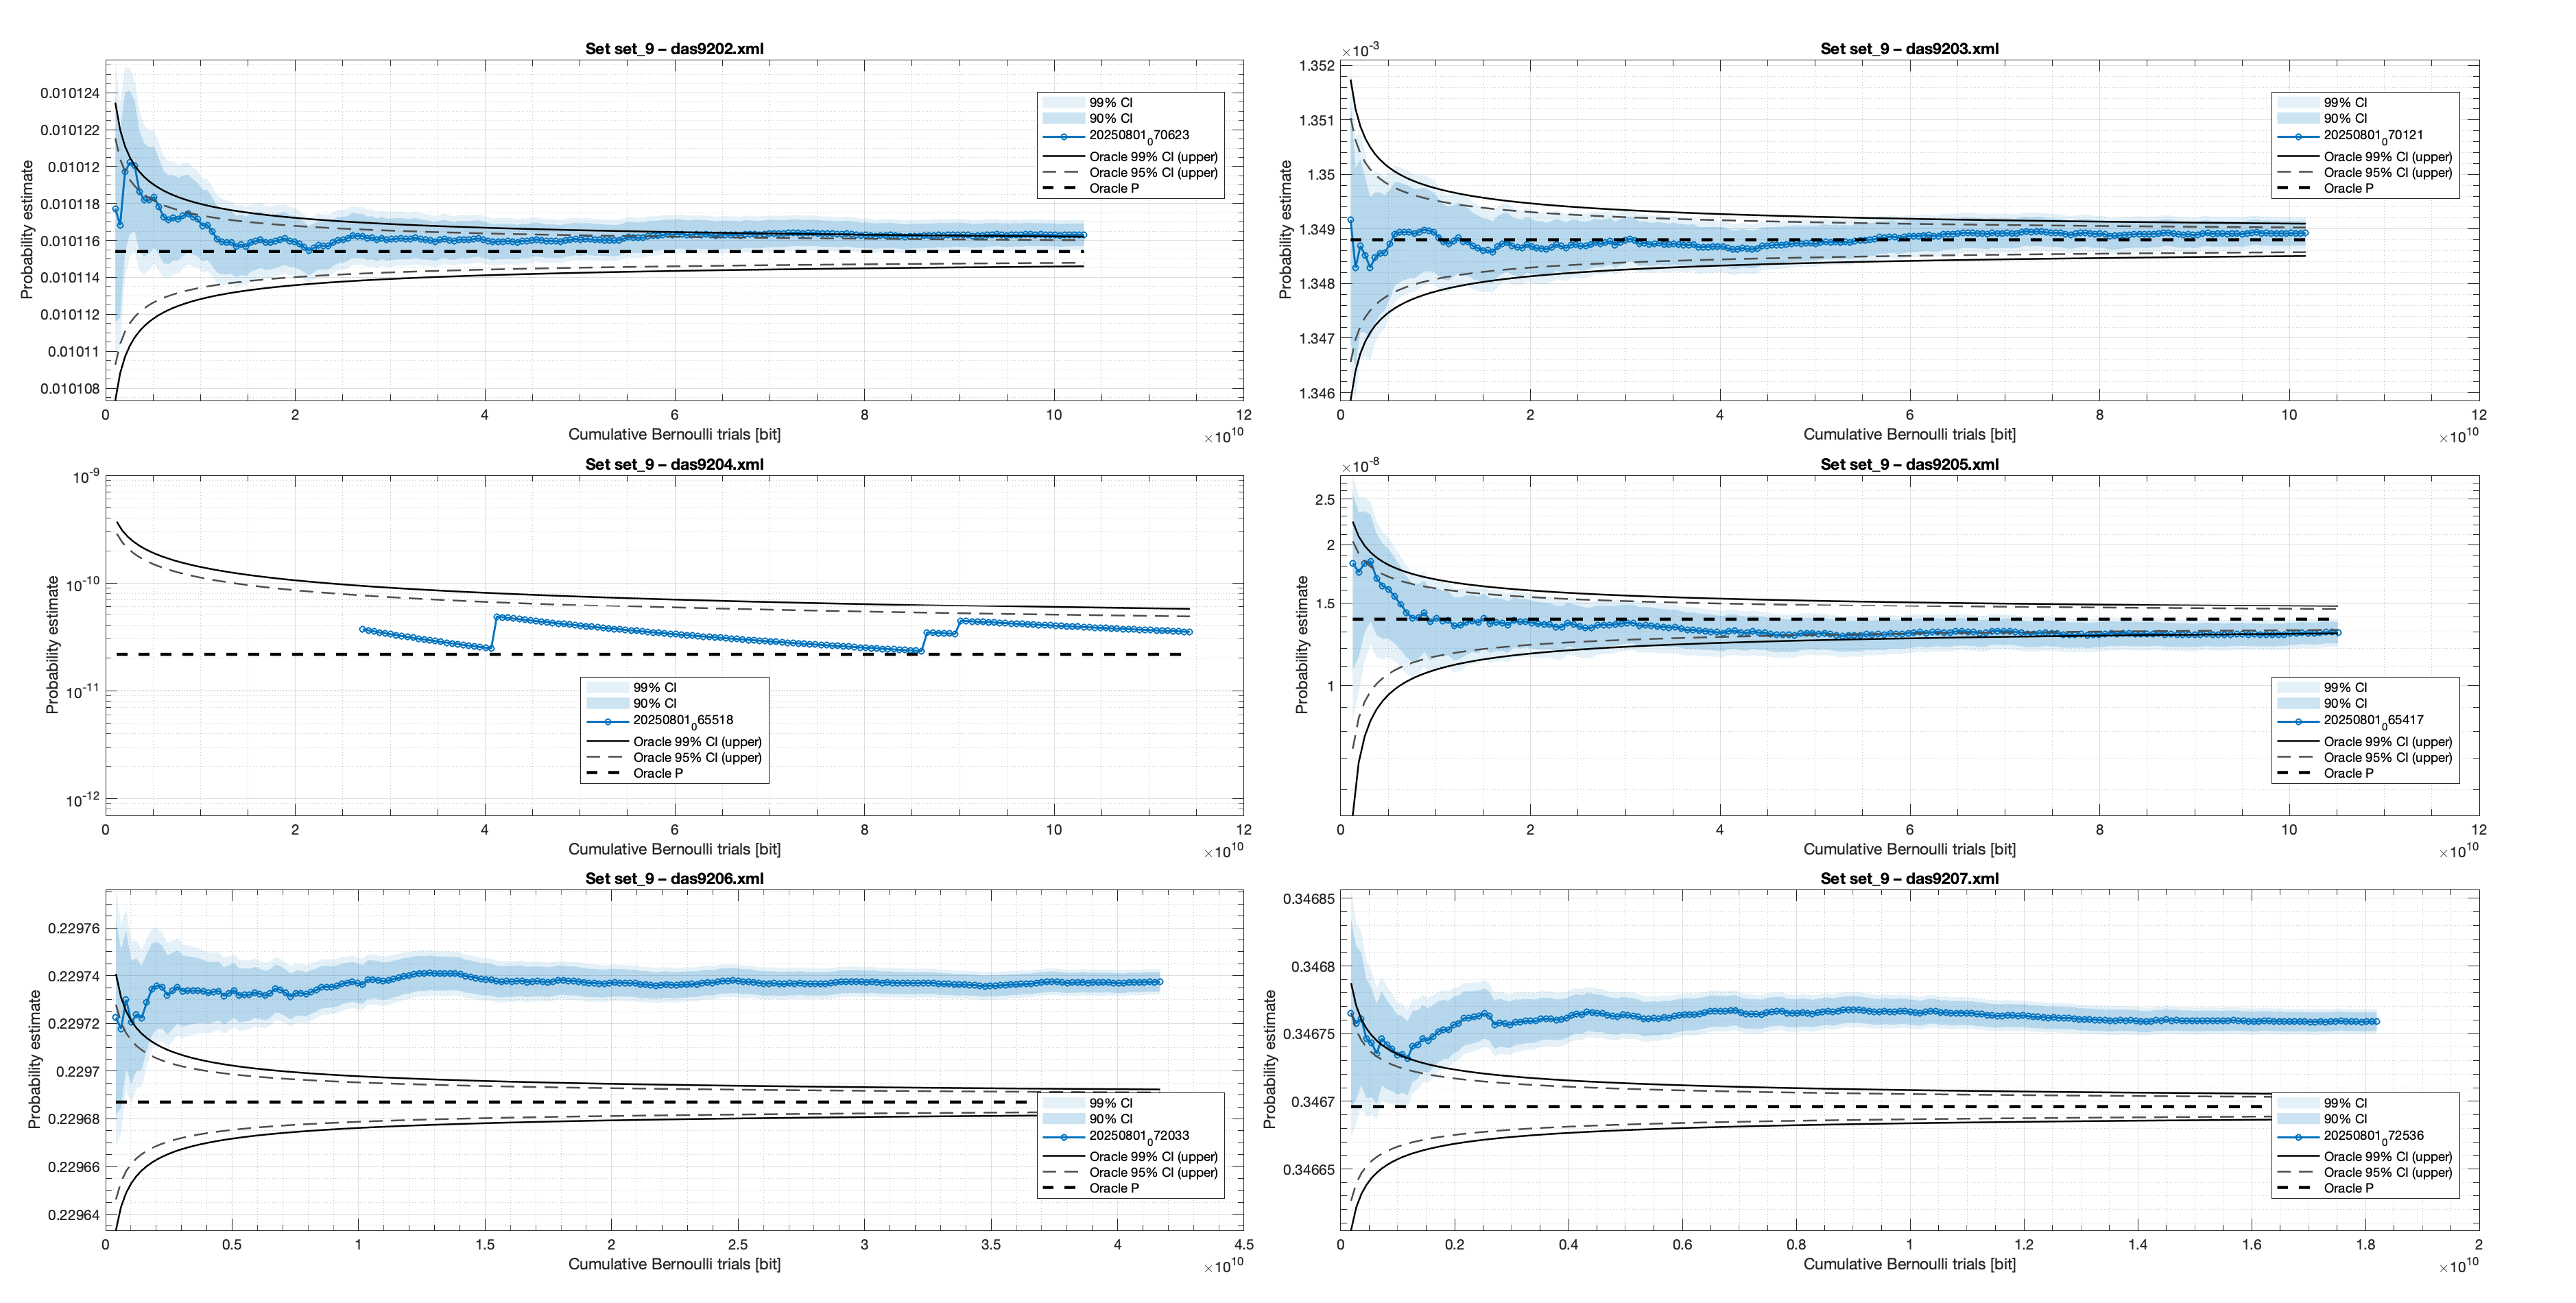
\includegraphics[height=1\textheight]{4_casestudy/conv_raw.eps}
    \label{fig:convergence_run_01}
\end{figure}
\end{frame}

\subsection{Convergence Runs, Comparison with MCUB, REA}
\begin{frame}
\begin{figure}[p]
    \centering
    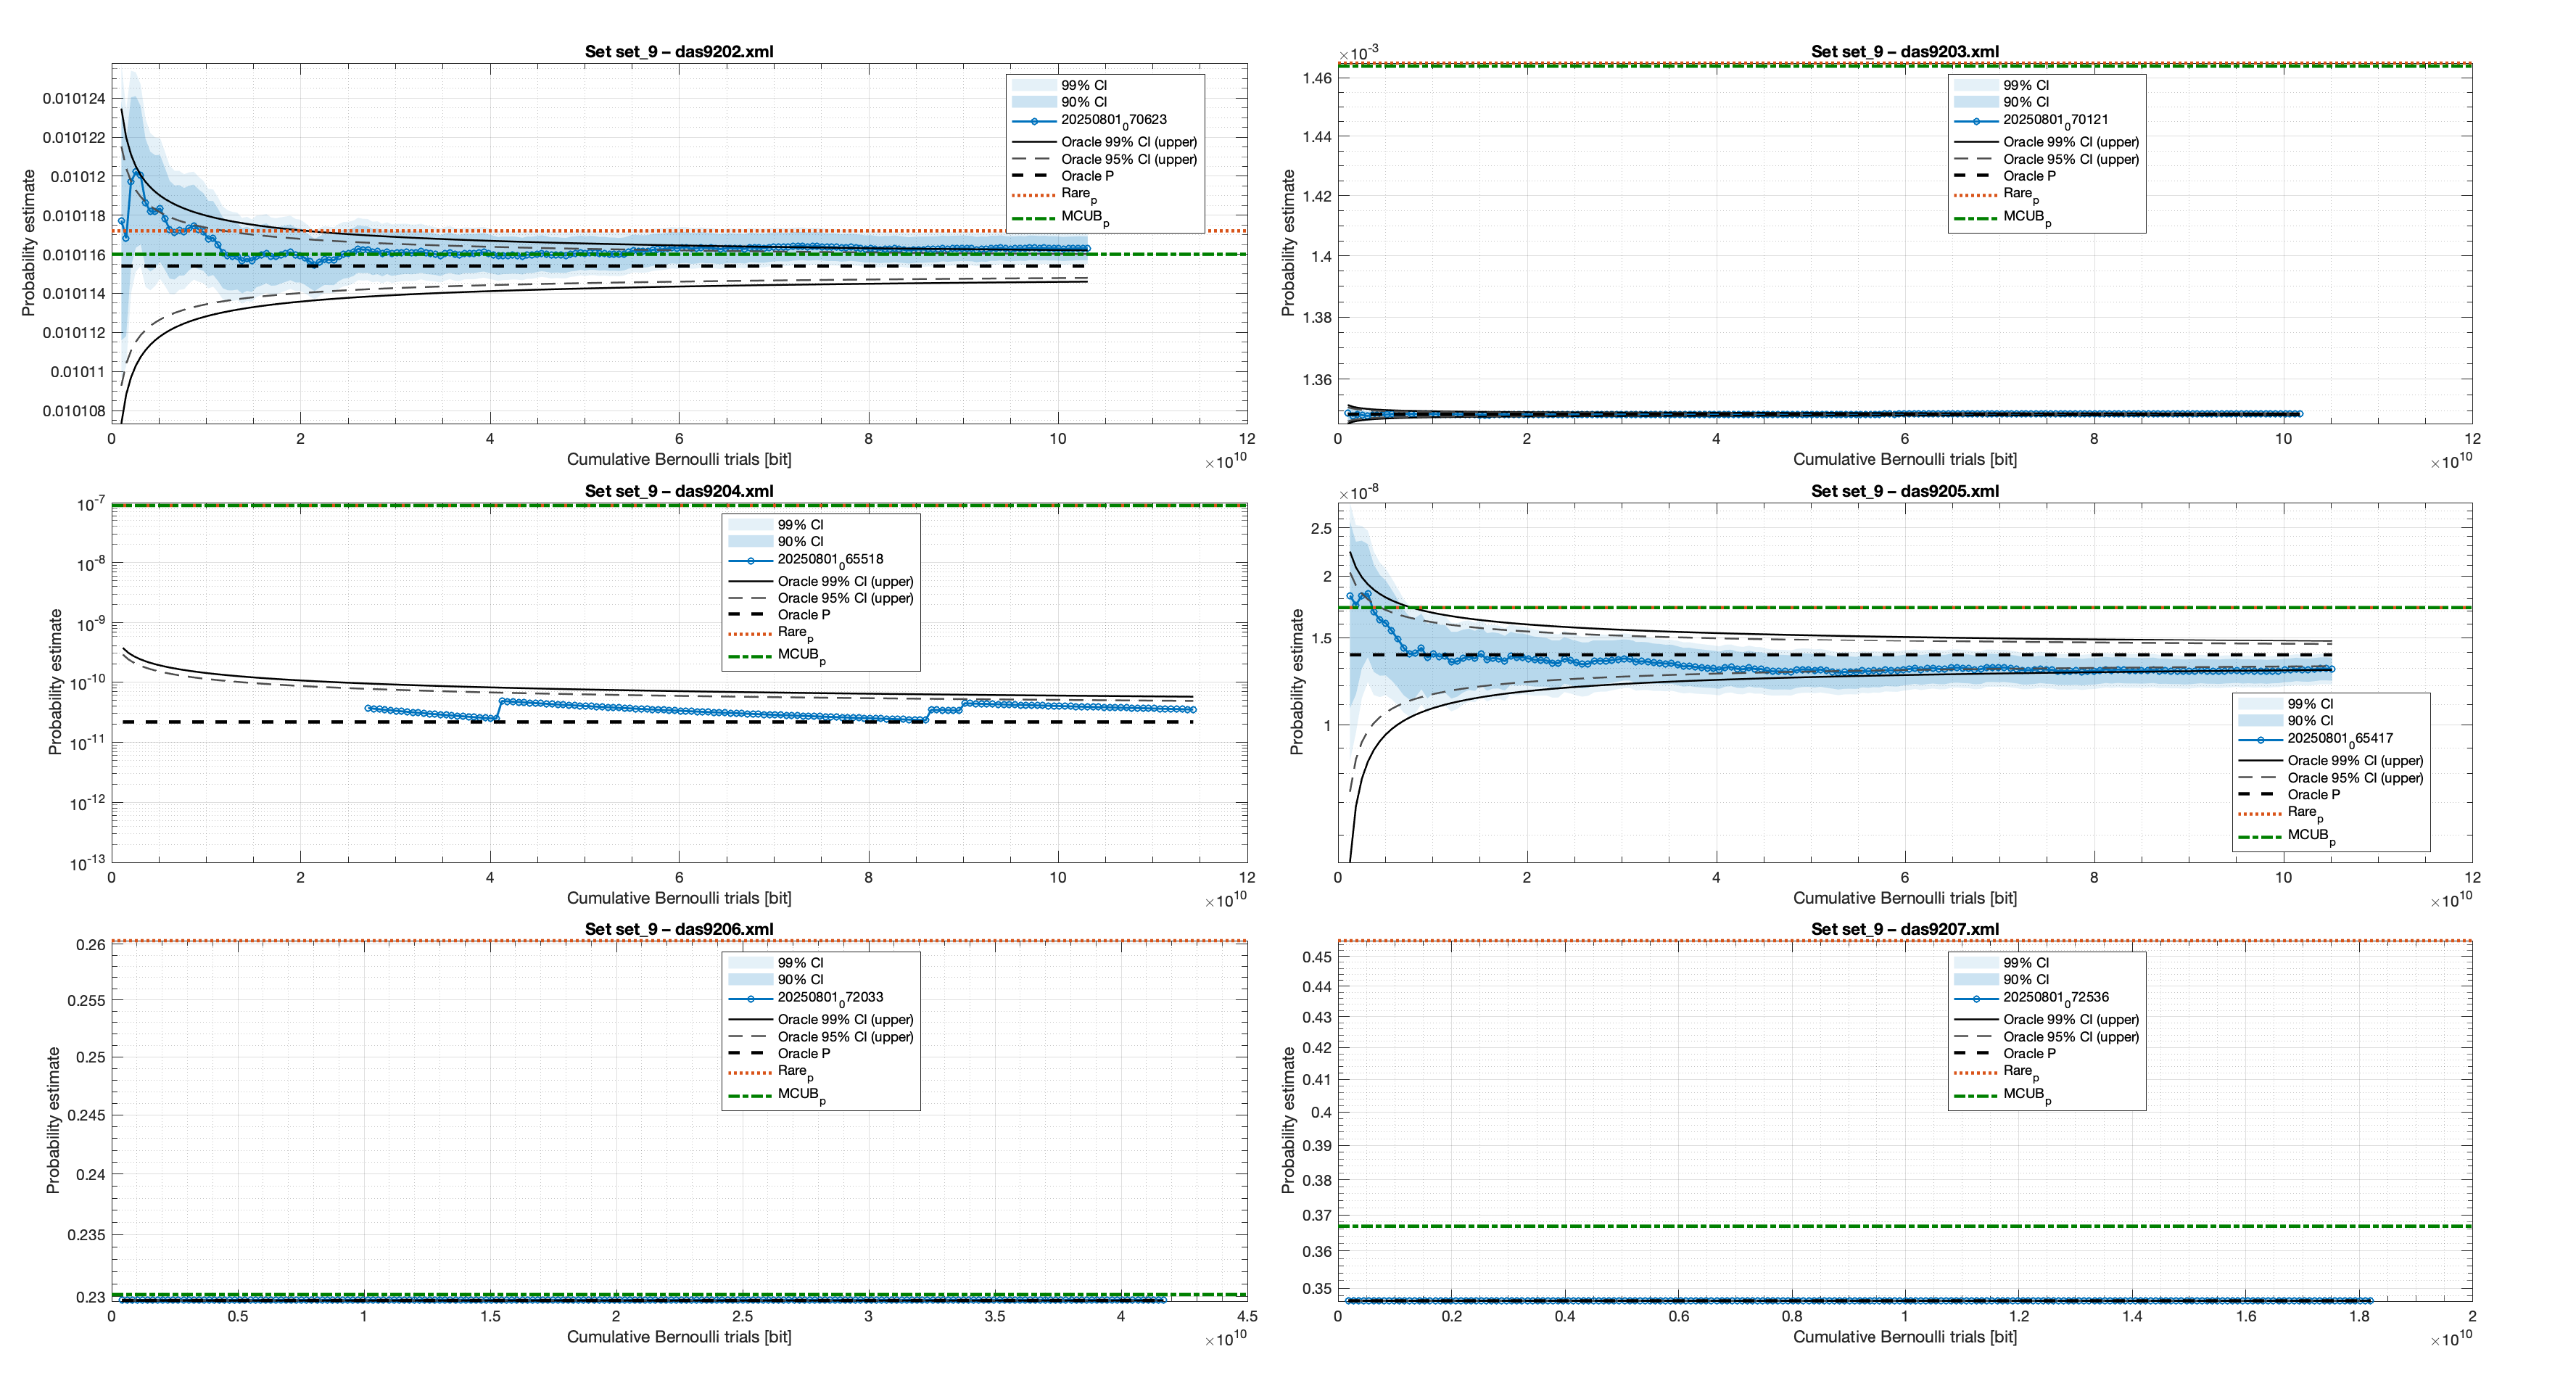
\includegraphics[height=1\textheight]{4_casestudy/conv_figeps.eps}
    \label{fig:convergence_run_01}
\end{figure}
\end{frame}

\subsection{Convergence Run -- Rare Event, Comparison with MCUB}
\begin{frame}
\begin{figure}[p]
    \centering
    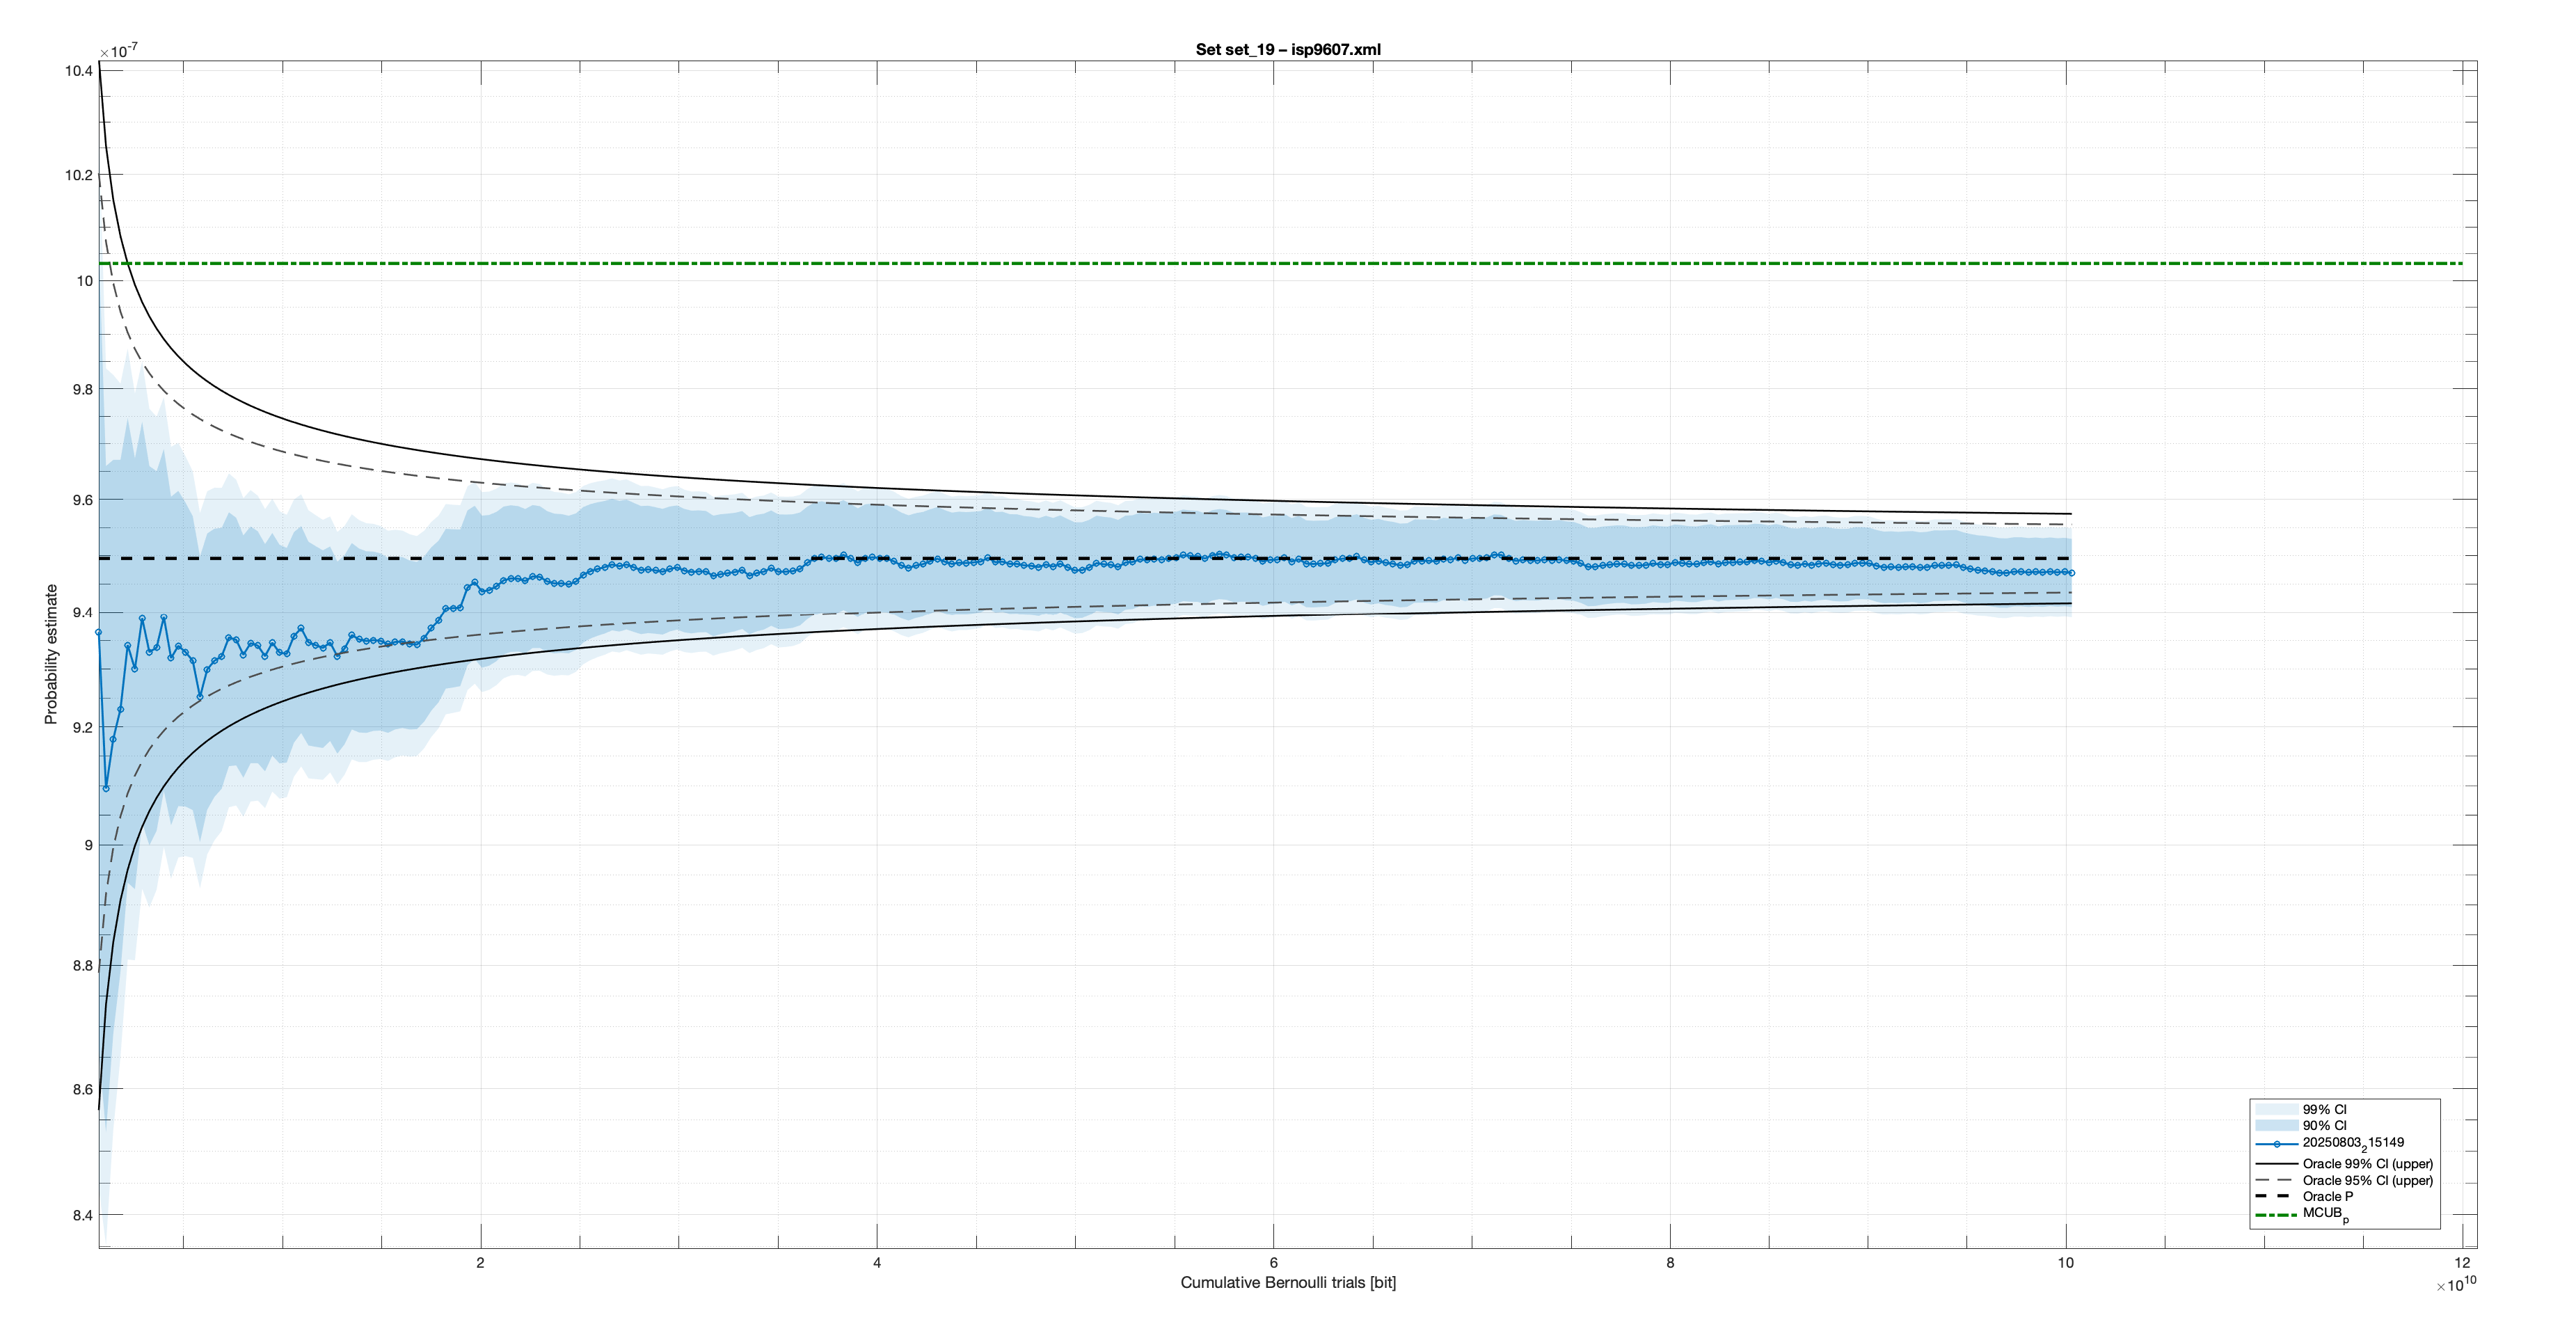
\includegraphics[height=0.9\textheight]{4_casestudy/conv_ips9607.eps}
    \label{fig:convergence_run_01}
\end{figure}
\end{frame}

\subsection{Convergence Free Run}
\begin{frame}
    \begin{figure}[h]
    \centering
    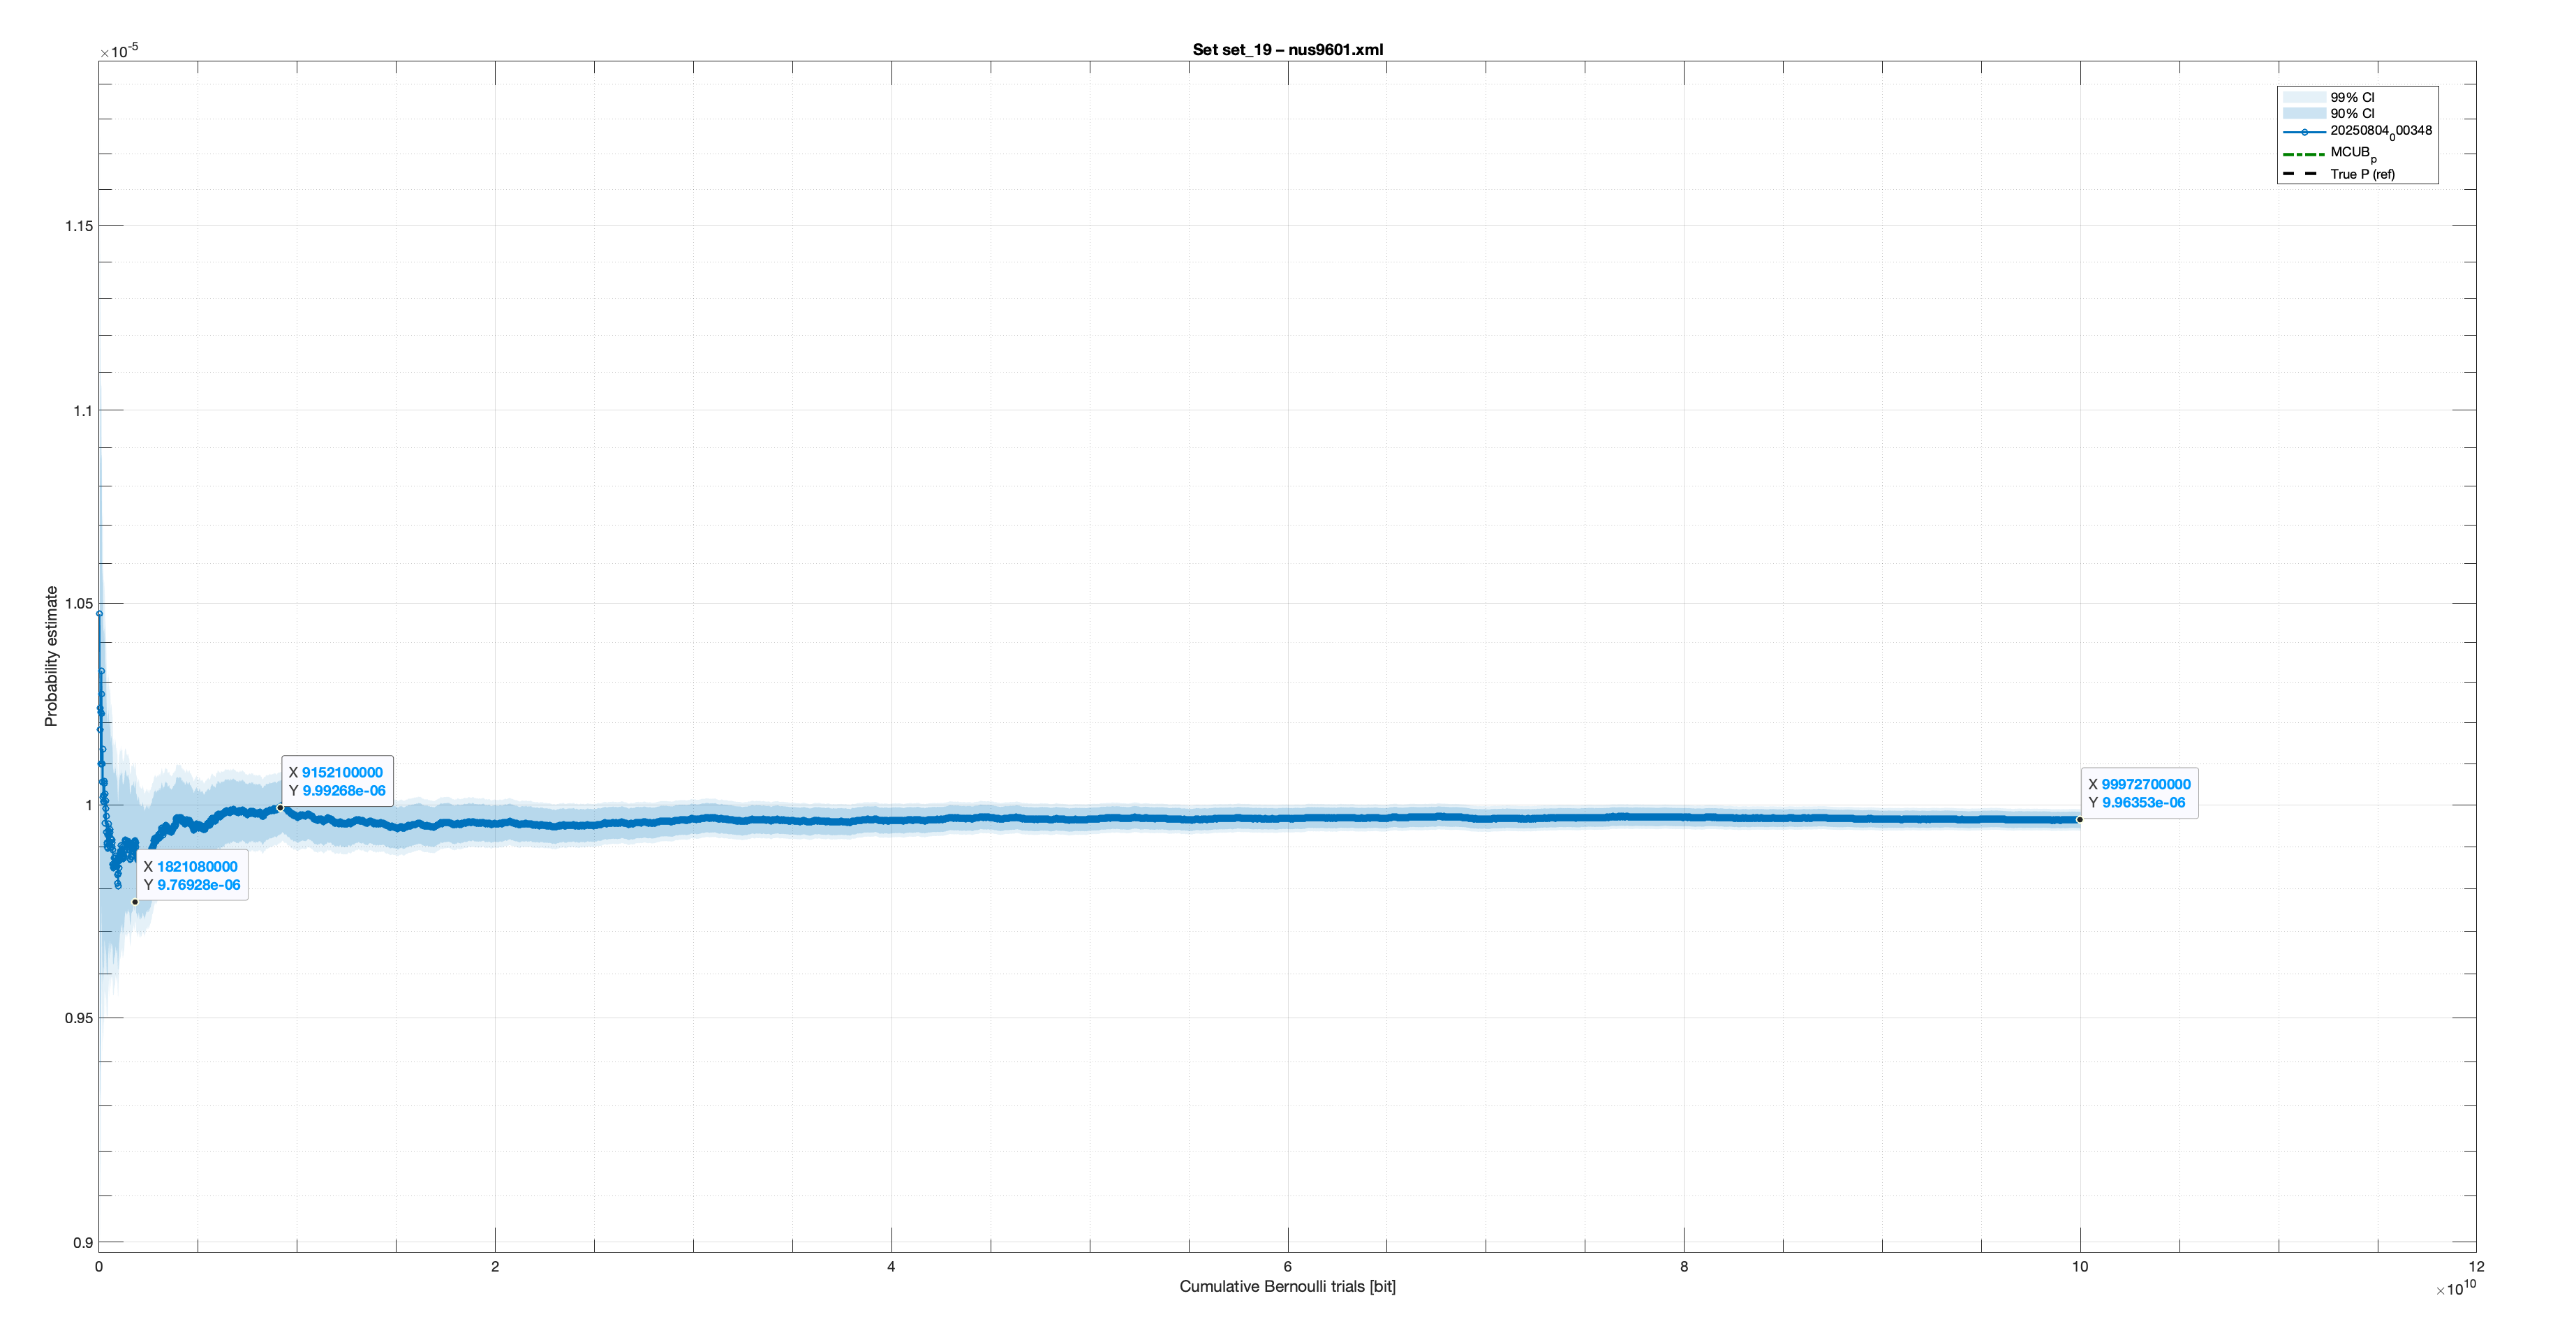
\includegraphics[width=1\textwidth]{4_casestudy/conv_nus9601.eps}
    \label{fig:rare}
\end{figure}
\end{frame}


\subsection{Aralia Fault Tree Data Set - Convergence for Rare Events}
\begin{frame}
    \input{4_casestudy/4_mae}
\end{frame}

% \subsection{Aralia Fault Tree Data Set - Throughput Benchmarks}
% \begin{frame}
%     \begin{figure}[h]
%     \centering
%     \includegraphics[width=0.9\textwidth]{4_casestudy/throughput/slides_nodes_vs_throughput.eps}
%     \caption{PDAG Node Count vs Throughput [bit/s]}
%     \label{fig:nodes_vs_throughput}
% \end{figure}
% \end{frame}




% \begin{frame}{Aralia Fault Tree Dataset}
% show the input dataset table\\
% \end{frame}

% \subsection{Results}
% \begin{frame}{Mar}
% show the input dataset table\\
% \end{frame}



\section{Research Objective 6: Domain Specific Extensions}
\begin{frame}
    \Large{\centerline{\textbf{Research Objective 6}}}
    \vspace{6pt}
    \large{\centerline{\textbf{Develop Importance Measures, Extend Common-Cause-Failure Analysis}}}
\end{frame}

% ------------------------------------
%  Frame 1 – Why Importance Measures?
% ------------------------------------
\subsection{Compute On-the-Fly Importance Measures}
\begin{frame}{Why Compute Importance Measures?}
  \begin{itemize}
    \item PRA stakeholders ask: \emph{“Which components matter most?”}
    \item Classical sensitivity indices (Birnbaum, Fussell–Vesely, RAW, RRW) quantify
          the change in top-event probability when basic-event reliabilities shift.
    \item Goal: embed these metrics \textbf{inside} the MC engine — no extra cut-set enumeration, no separate gate passes.
  \end{itemize}
  \vspace{6pt}
  \centering
  % \includegraphics[width=0.65\linewidth]{1_concepts/importance_cartoon.pdf} % placeholder figure
\end{frame}

% ------------------------------------
%  Frame 2 – Definitions
% ------------------------------------
\begin{frame}{Classical Definitions (per basic event $i$)}
\footnotesize
\begin{tabular}{l p{12cm}}
\toprule
\textbf{Measure} & \textbf{Analytical Definition}\\
\midrule
Birnbaum (MIF) & $\displaystyle \operatorname{MIF}_i = \frac{\partial P_{\text{top}}}{\partial p_i}$\\[4pt]
Critical (CIF) & $\displaystyle \operatorname{CIF}_i = \operatorname{MIF}_i\,\frac{p_i}{P_{\text{top}}}$\\[4pt]
Diagnostic (DIF) & $\displaystyle \operatorname{DIF}_i = \frac{\Pr\{X_i=1\,\wedge\,Z=1\}}{p_i P_{\text{top}}}$\\[4pt]
RAW / RRW & Risk achievement / reduction worth — counterfactual probabilities when $X_i$ forced to $1$ or $0$\\
\bottomrule
\end{tabular}
\pause
\vspace{4pt}
\textbf{Key insight:}\; All measures reduce to combinations of three sample proportions:
\[ \widehat p_i = \frac{s_i}{n},\quad \widehat p_0=\frac{s_0}{n},\quad \widehat p_{0,i}=\frac{s_{0,i}}{n}. \]
\end{frame}

% ------------------------------------
%  Frame 3 – MC Estimation & Convergence
% ------------------------------------
\begin{frame}{MC Estimation with Minimal Sufficient Statistics}
    \textbf{Per-iteration tallies}
    \[
      s_i \!\leftarrow\! s_i + \operatorname{popcount}(X_i),\quad
      s_0 \!\leftarrow\! s_0 + \operatorname{popcount}(Z),\quad
      s_{0,i} \!\leftarrow\! s_{0,i} + \operatorname{popcount}(X_i \,\&\, Z).
    \]
    Only \textbf{one} extra bitwise \texttt{AND} + \texttt{popcount} per basic event.

    \vspace{4pt}
    \textbf{Estimator example (Birnbaum):}
    \[
      \widehat{\operatorname{MIF}}_i =
      \frac{\widehat p_{0,i} - \widehat p_0\widehat p_i}
           {\widehat p_i(1-\widehat p_i)}.
    \]
\end{frame}

% ------------------------------------
%  Frame 3 – MC Estimation & Convergence
% ------------------------------------
\begin{frame}{MC Estimation with Minimal Sufficient Statistics}
    \begin{block}{Convergence Guarantee}
      Each counter is a sum of $n=TN$ independent Bernoulli trials:
      \[
        \sqrt{n}\,(\widehat p - p) \;\xrightarrow{d}\; \mathcal N(0,\,p(1-p)).
      \]
      By the delta method the importance estimators inherit $\mathcal O(n^{-1/2})$ variance.

      \vspace{4pt}
      \emph{Same composite stopping rule} (half-width, credible interval, info-gain) thus applies without modification.
    \end{block}
\end{frame}


\subsection{Common-Cause Failure (CCF) in Monte-Carlo}

% ------------------------------------
%  Frame 1 – Why Common-Cause Failure Modelling?
% ------------------------------------
\begin{frame}{Motivation: Common-Cause Failures}
  \begin{itemize}
    \item Independent failure assumption breaks down when components share hidden dependencies (environment, manufacturing defects, etc.).
    \item Neglecting CCFs can under-predict top-event probability by orders of magnitude.
    \item Goal: incorporate parametric CCF models \emph{without} disrupting the bit-parallel Monte-Carlo pipeline.
  \end{itemize}
  \vspace{4pt}
\end{frame}

% ------------------------------------
%  Frame 2 – Embedding CCF Groups in the PDAG
% ------------------------------------
\begin{frame}{Graph Construction for a CCF Group $\mathcal C$}
  \footnotesize
  \begin{enumerate}
    \item \textbf{Scale independent leaves.}  Each basic event $c_i\in\mathcal C$ keeps an independent probability $(1-\lambda_{\text{ccf}})\,p_{c_i}$.   
    \item \textbf{Insert CCF trigger variable} $S_{\mathcal C}$ with failure probability $\lambda_{\text{ccf}} = \sum_{k\ge2} \pi_{\mathcal C,k}$.  
    \item \textbf{CCF-root gate} $G_{\mathcal C}= S_{\mathcal C}\lor c_1\lor\dots\lor c_m$ routes either independent or common shock to the rest of the graph.
    \item (Optional) \textbf{Multiplicity shadow gates} $H^{(k)}_{\mathcal C}$ realize models that distinguish the number $k$ of simultaneously failed components.
  \end{enumerate}
  \vspace{2pt}
  \begin{block}{Key property}
    All new nodes are \emph{gates}; the set of basic events is unchanged, so the Monte-Carlo sampling kernel remains untouched.
  \end{block}
\end{frame}

% ------------------------------------
%  Frame 3 – Monte-Carlo Evaluation & Convergence
% ------------------------------------
\begin{frame}{MC Treatment and Convergence Guarantees}
  \begin{columns}[T]
    \column{0.50\textwidth}
    \textbf{Sampling logic}
    \begin{itemize}
      \item Leaves $\{S_{\mathcal C},c_1,\dots,c_m\}$ are sampled \emph{independently}.  Correlation enters only via logic connectivity.
      \item Same bit-packing kernel, same PRNG counters – zero performance overhead.
      \item Trigger variable firing forces simultaneous bits in the shadow gate; implemented by one extra OR reduction.
    \end{itemize}
    \column{0.50\textwidth}
    \begin{block}{Unbiasedness & Variance}
      Indicator $Z$ of any top-level node is still a Bernoulli random variable.
      \[
        \operatorname{Var}[Z] = P(1-P),\qquad P=\Pr[Z=1].
      \]
      Therefore all proofs for half-width, Bayesian interval, and information-gain criteria remain valid \textbf{unchanged}.  CCF merely shifts $P$.
    \end{block}
  \end{columns}
  \vspace{4pt}
  \textbf{Take-away:} CCF groups integrate into MC with \emph{zero} sampler modification; convergence diagnostics from Research Objective 4 apply verbatim.
\end{frame}



\section{Research Objective 5: Case Studies and Benchmarks}
\begin{frame}
    \Large{\centerline{\textbf{Research Objective 5}}}
    \vspace{6pt}
    \large{\centerline{\textbf{Case Studies and Benchmarks}}}
\end{frame}

\subsection{Aralia Fault Tree Data Set}
\begin{frame}[t]
\frametitle{Overview: Aralia Dataset}
\begin{itemize}
  \item \textbf{Dataset Composition:} The Aralia collection consists of 43 distinct fault trees, each with varying numbers of basic events (BEs), gate types (AND, OR, K/N, XOR), and minimal cut-set counts.  
  \item \textbf{Diverse Problem Sizes:} Small trees (e.g.\ 25--32 BEs) through large models with over 1{,}500 BEs.  
  \item \textbf{Wide Probability Range:} Top-event probabilities spanning from rare events near \(10^{-13}\) to fairly likely failures with probability above 0.7.  
  \item \textbf{Model Variability:} Some trees are primarily AND/OR, others incorporate more advanced gates (K/N, XOR, NOT), providing thorough coverage of typical (and atypical) fault tree logic structures.
\end{itemize}
\end{frame}

\begin{frame}[allowframebreaks]
    \input{4_casestudy/3_table_aralia_ft_dataset}
\end{frame}

\subsection{Benchmarking Procedure}
\begin{frame}[t]
\frametitle{Benchmarking Setup: Hardware and Environment}
\begin{itemize}
  \item \textbf{Target Hardware:}
    \begin{itemize}
      \item GPU: NVIDIA\textsuperscript{\textregistered} GeForce GTX 1660 SUPER (6\,GB GDDR6, 1{,}408 CUDA cores).
      \item CPU: Intel\textsuperscript{\textregistered} Core\textsuperscript{TM} i7-10700 (2.90\,GHz, turbo-boost, hyperthreading).
    \end{itemize}
  \item \textbf{Software Stack:}
    \begin{itemize}
      \item SYCL-based (AdaptiveCpp/HipSYCL), with LLVM-IR JIT for kernel compilation.
      \item Compiler optimization at \texttt{-O3} for efficient code generation.
      \item Repeated runs (5+) to mitigate transient variations.
    \end{itemize}
  \item \textbf{Measured Time:} Includes entire wall-clock duration, from host-device transfers and JIT compilation to final result collection.
\end{itemize}
\end{frame}

\subsection{Accuracy Benchmarks}
\begin{frame}
    \begin{figure}[h]
    \centering
    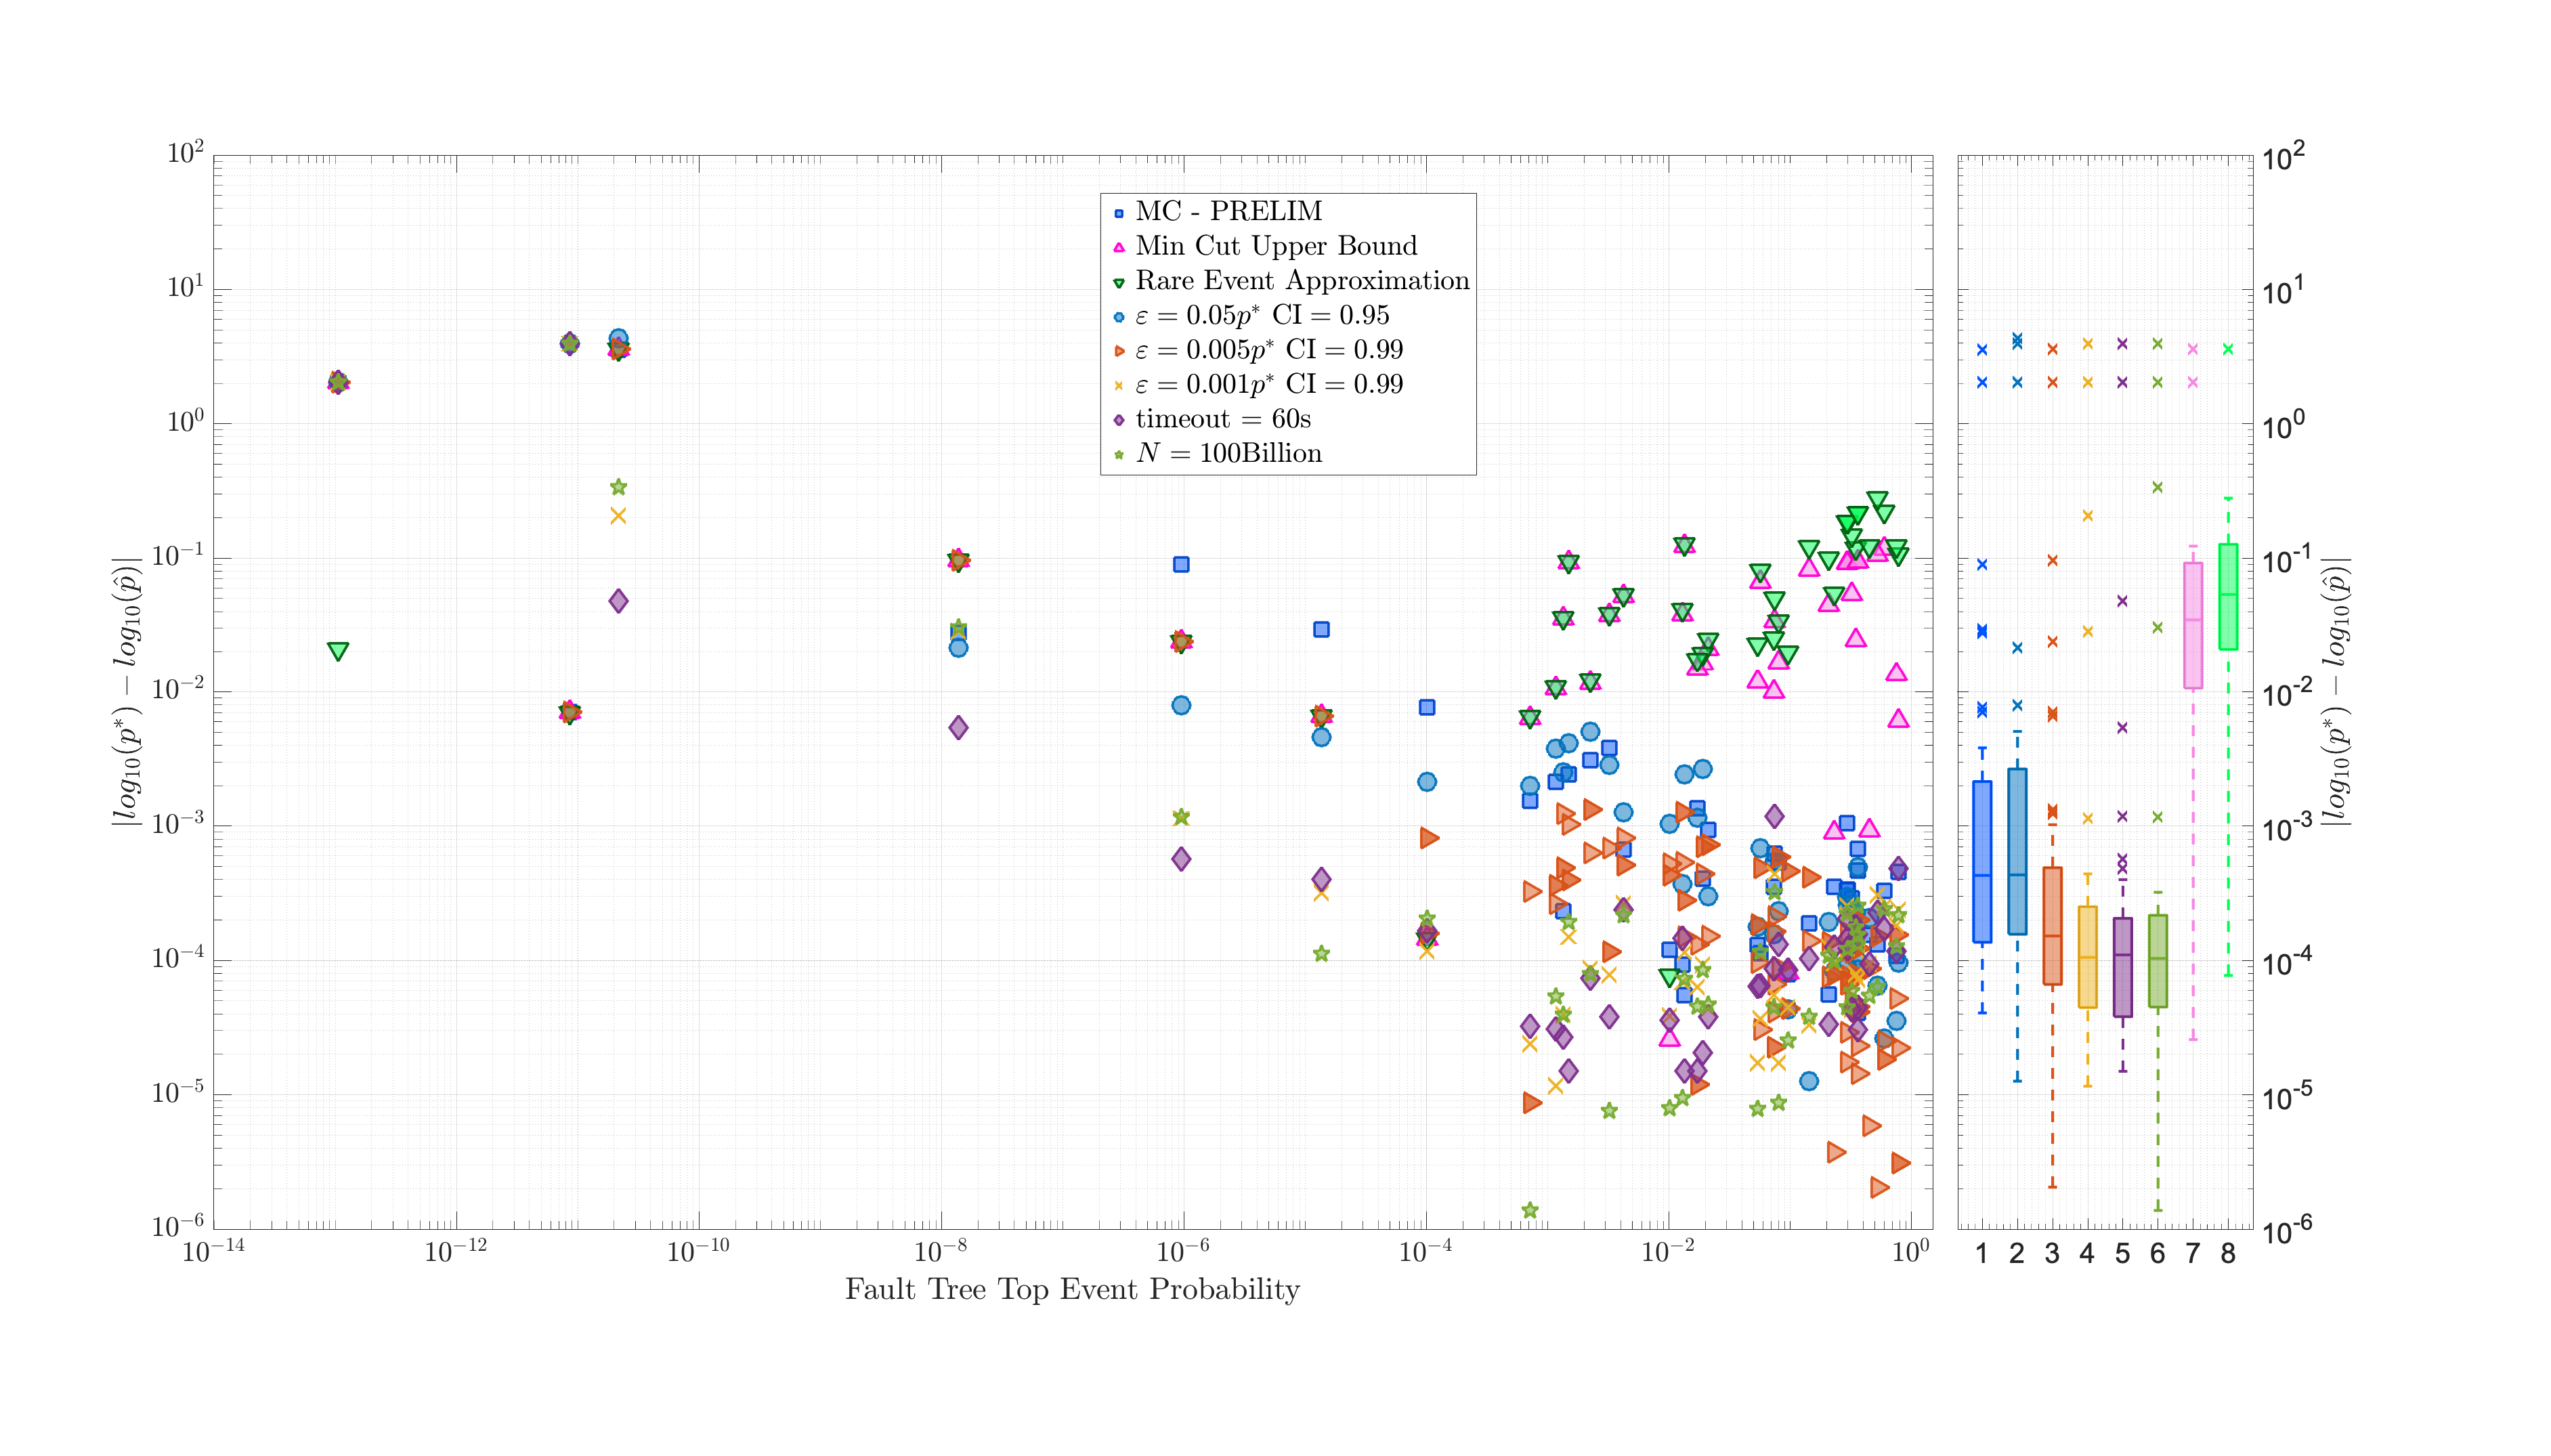
\includegraphics[height=1.1\textheight]{4_casestudy/abs_err.eps}
    \label{fig:mae_vs_logp}
\end{figure}
\end{frame}

\subsection{Accuracy vs. Time to Convergence}
\begin{frame}
\begin{figure}[p]
    \centering
    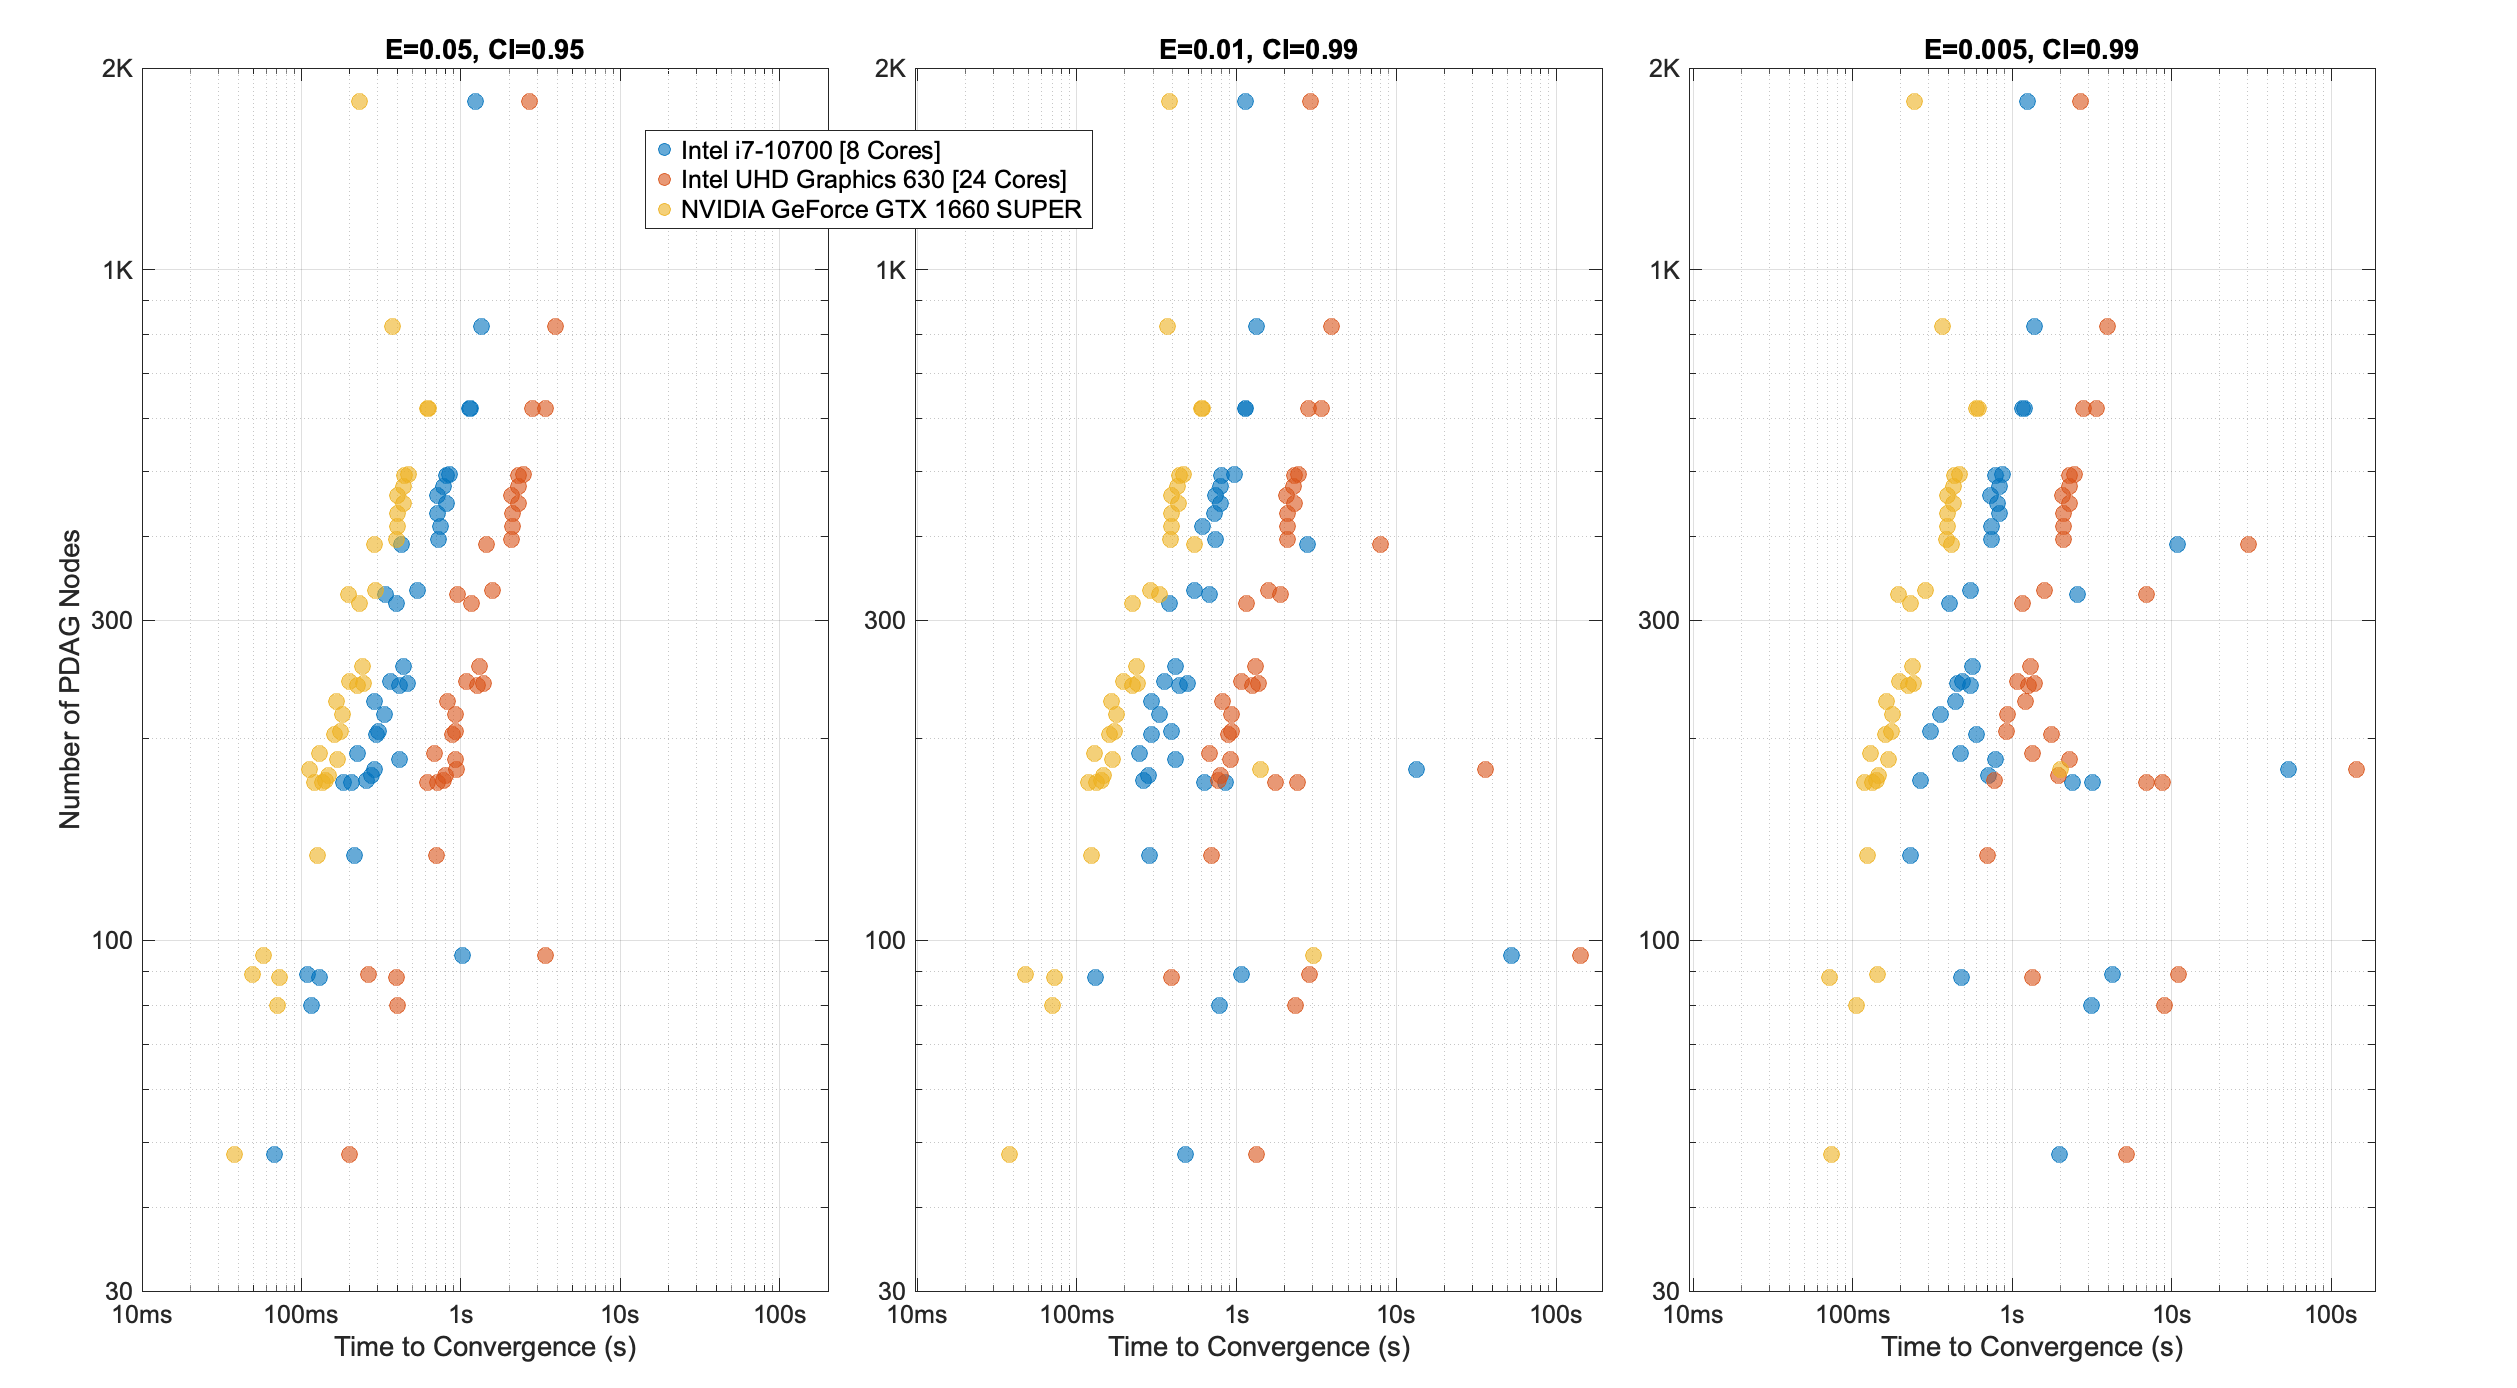
\includegraphics[height=1\textheight]{4_casestudy/throughput/slides_nodes_vs_convergence.eps}
    \caption{Time to convergence for different accuracy targets.}
    \label{fig:nodes_vs_convergence}
\end{figure}
\end{frame}

\subsection{Convergence Runs}
\begin{frame}
\begin{figure}[p]
    \centering
    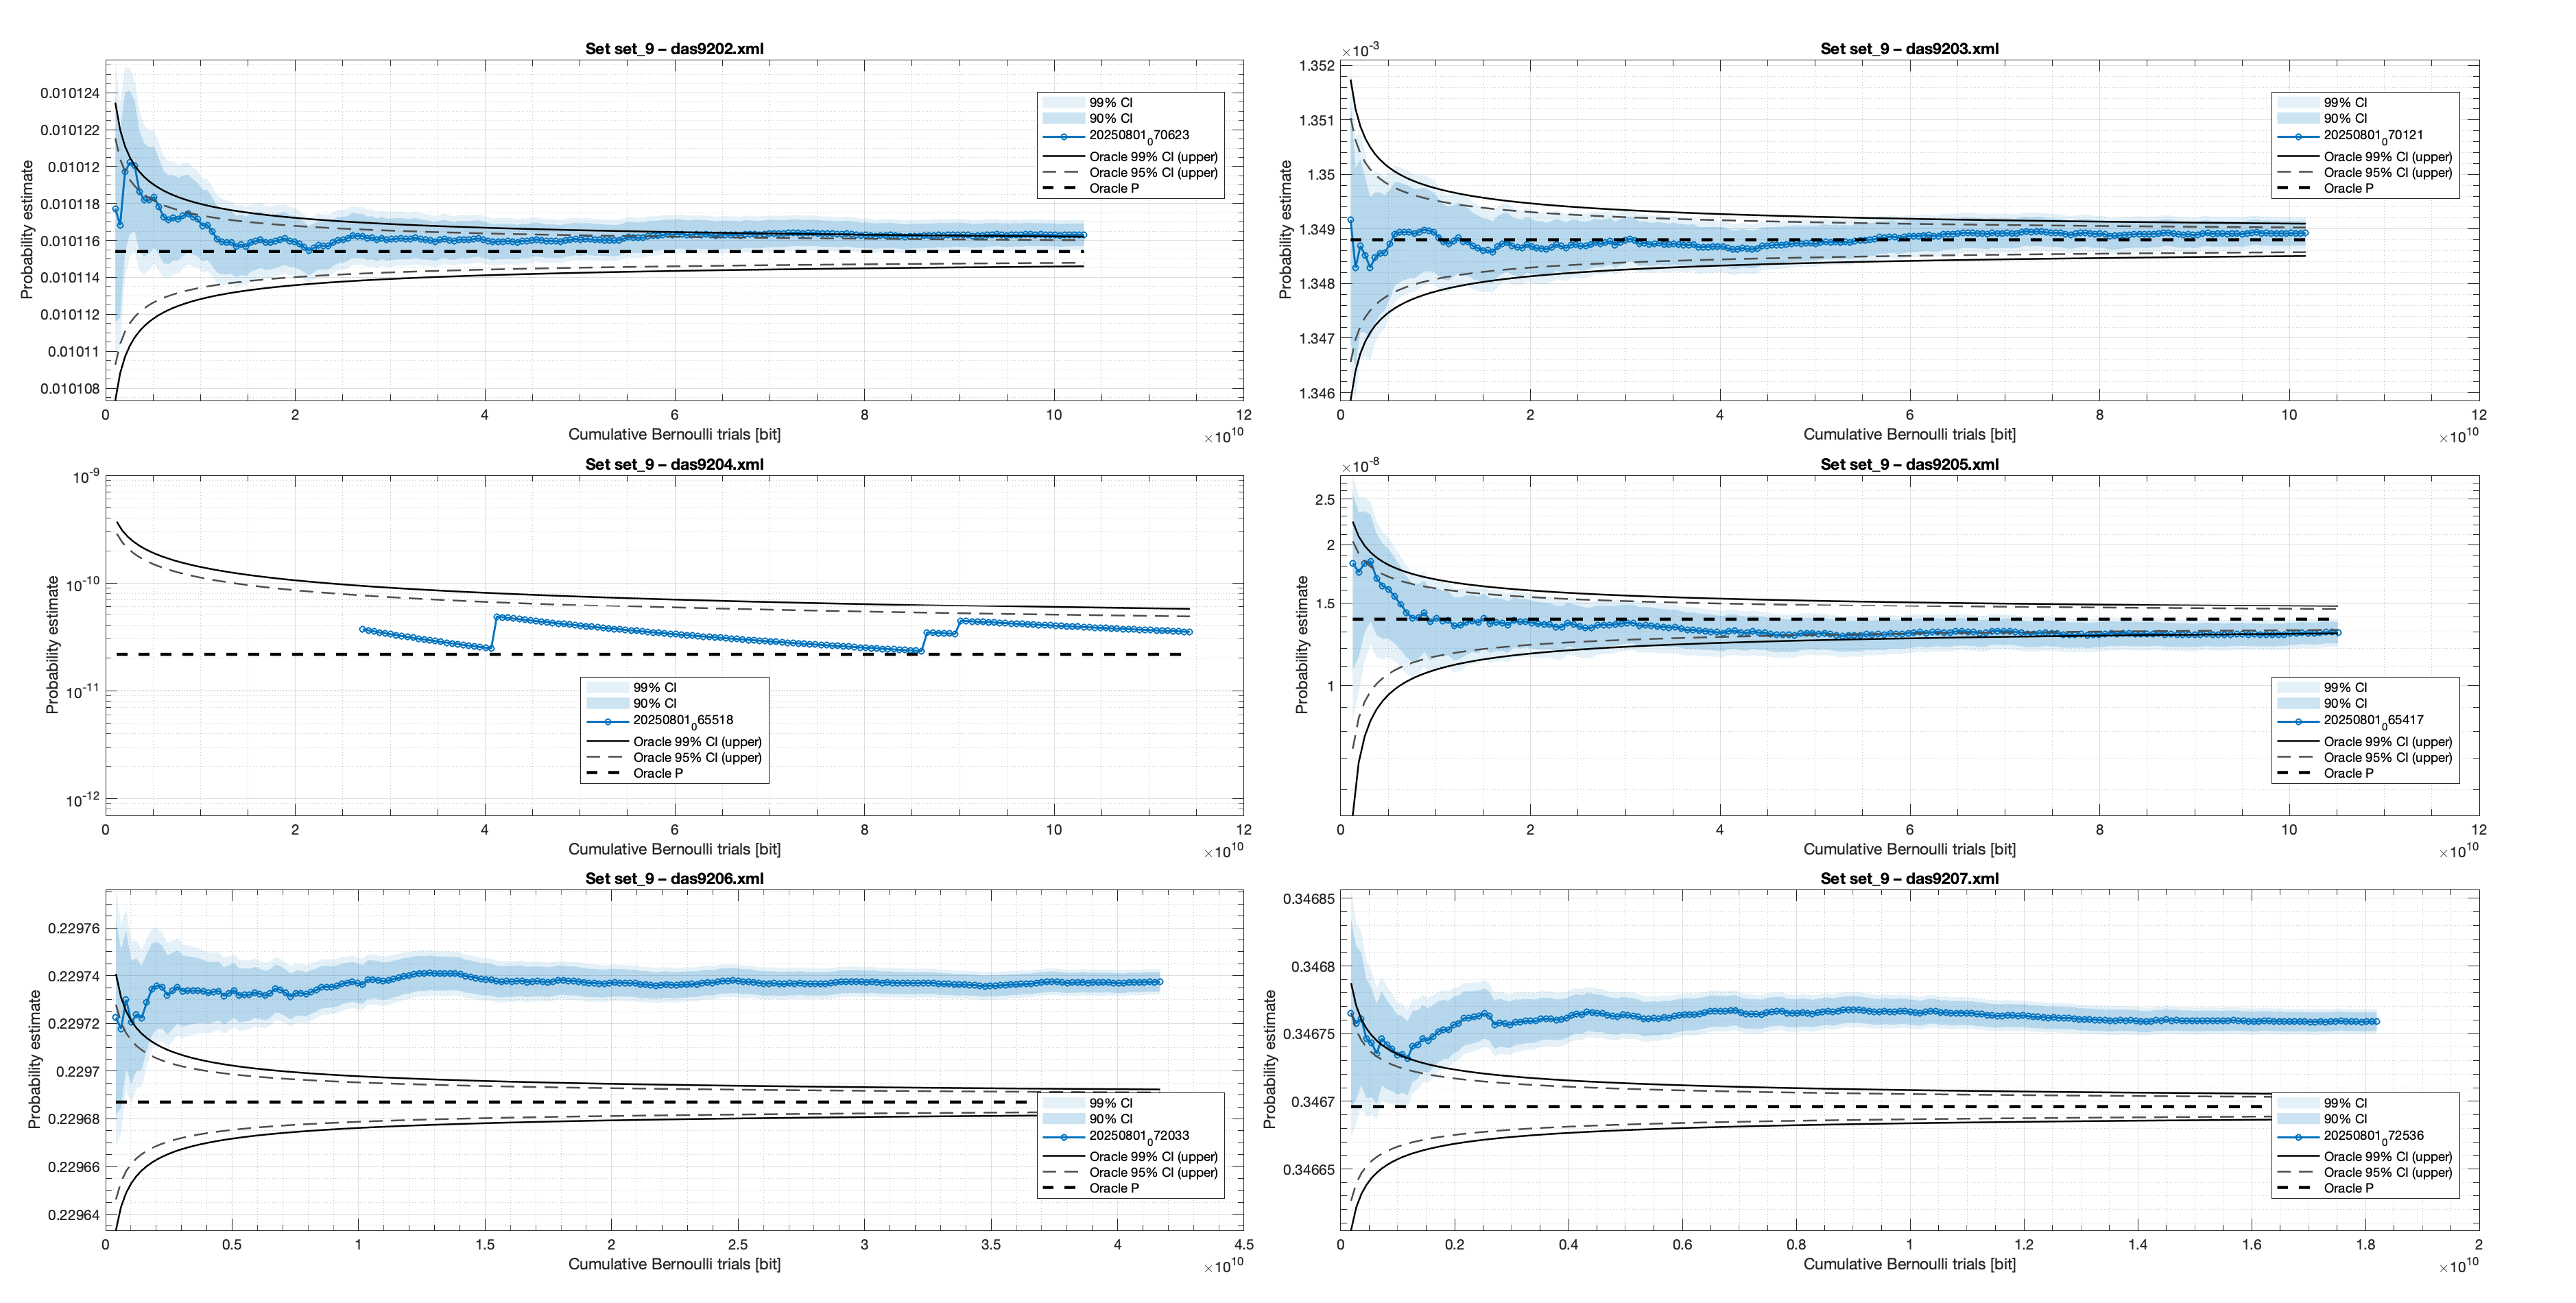
\includegraphics[height=1\textheight]{4_casestudy/conv_raw.eps}
    \label{fig:convergence_run_01}
\end{figure}
\end{frame}

\subsection{Convergence Runs, Comparison with MCUB, REA}
\begin{frame}
\begin{figure}[p]
    \centering
    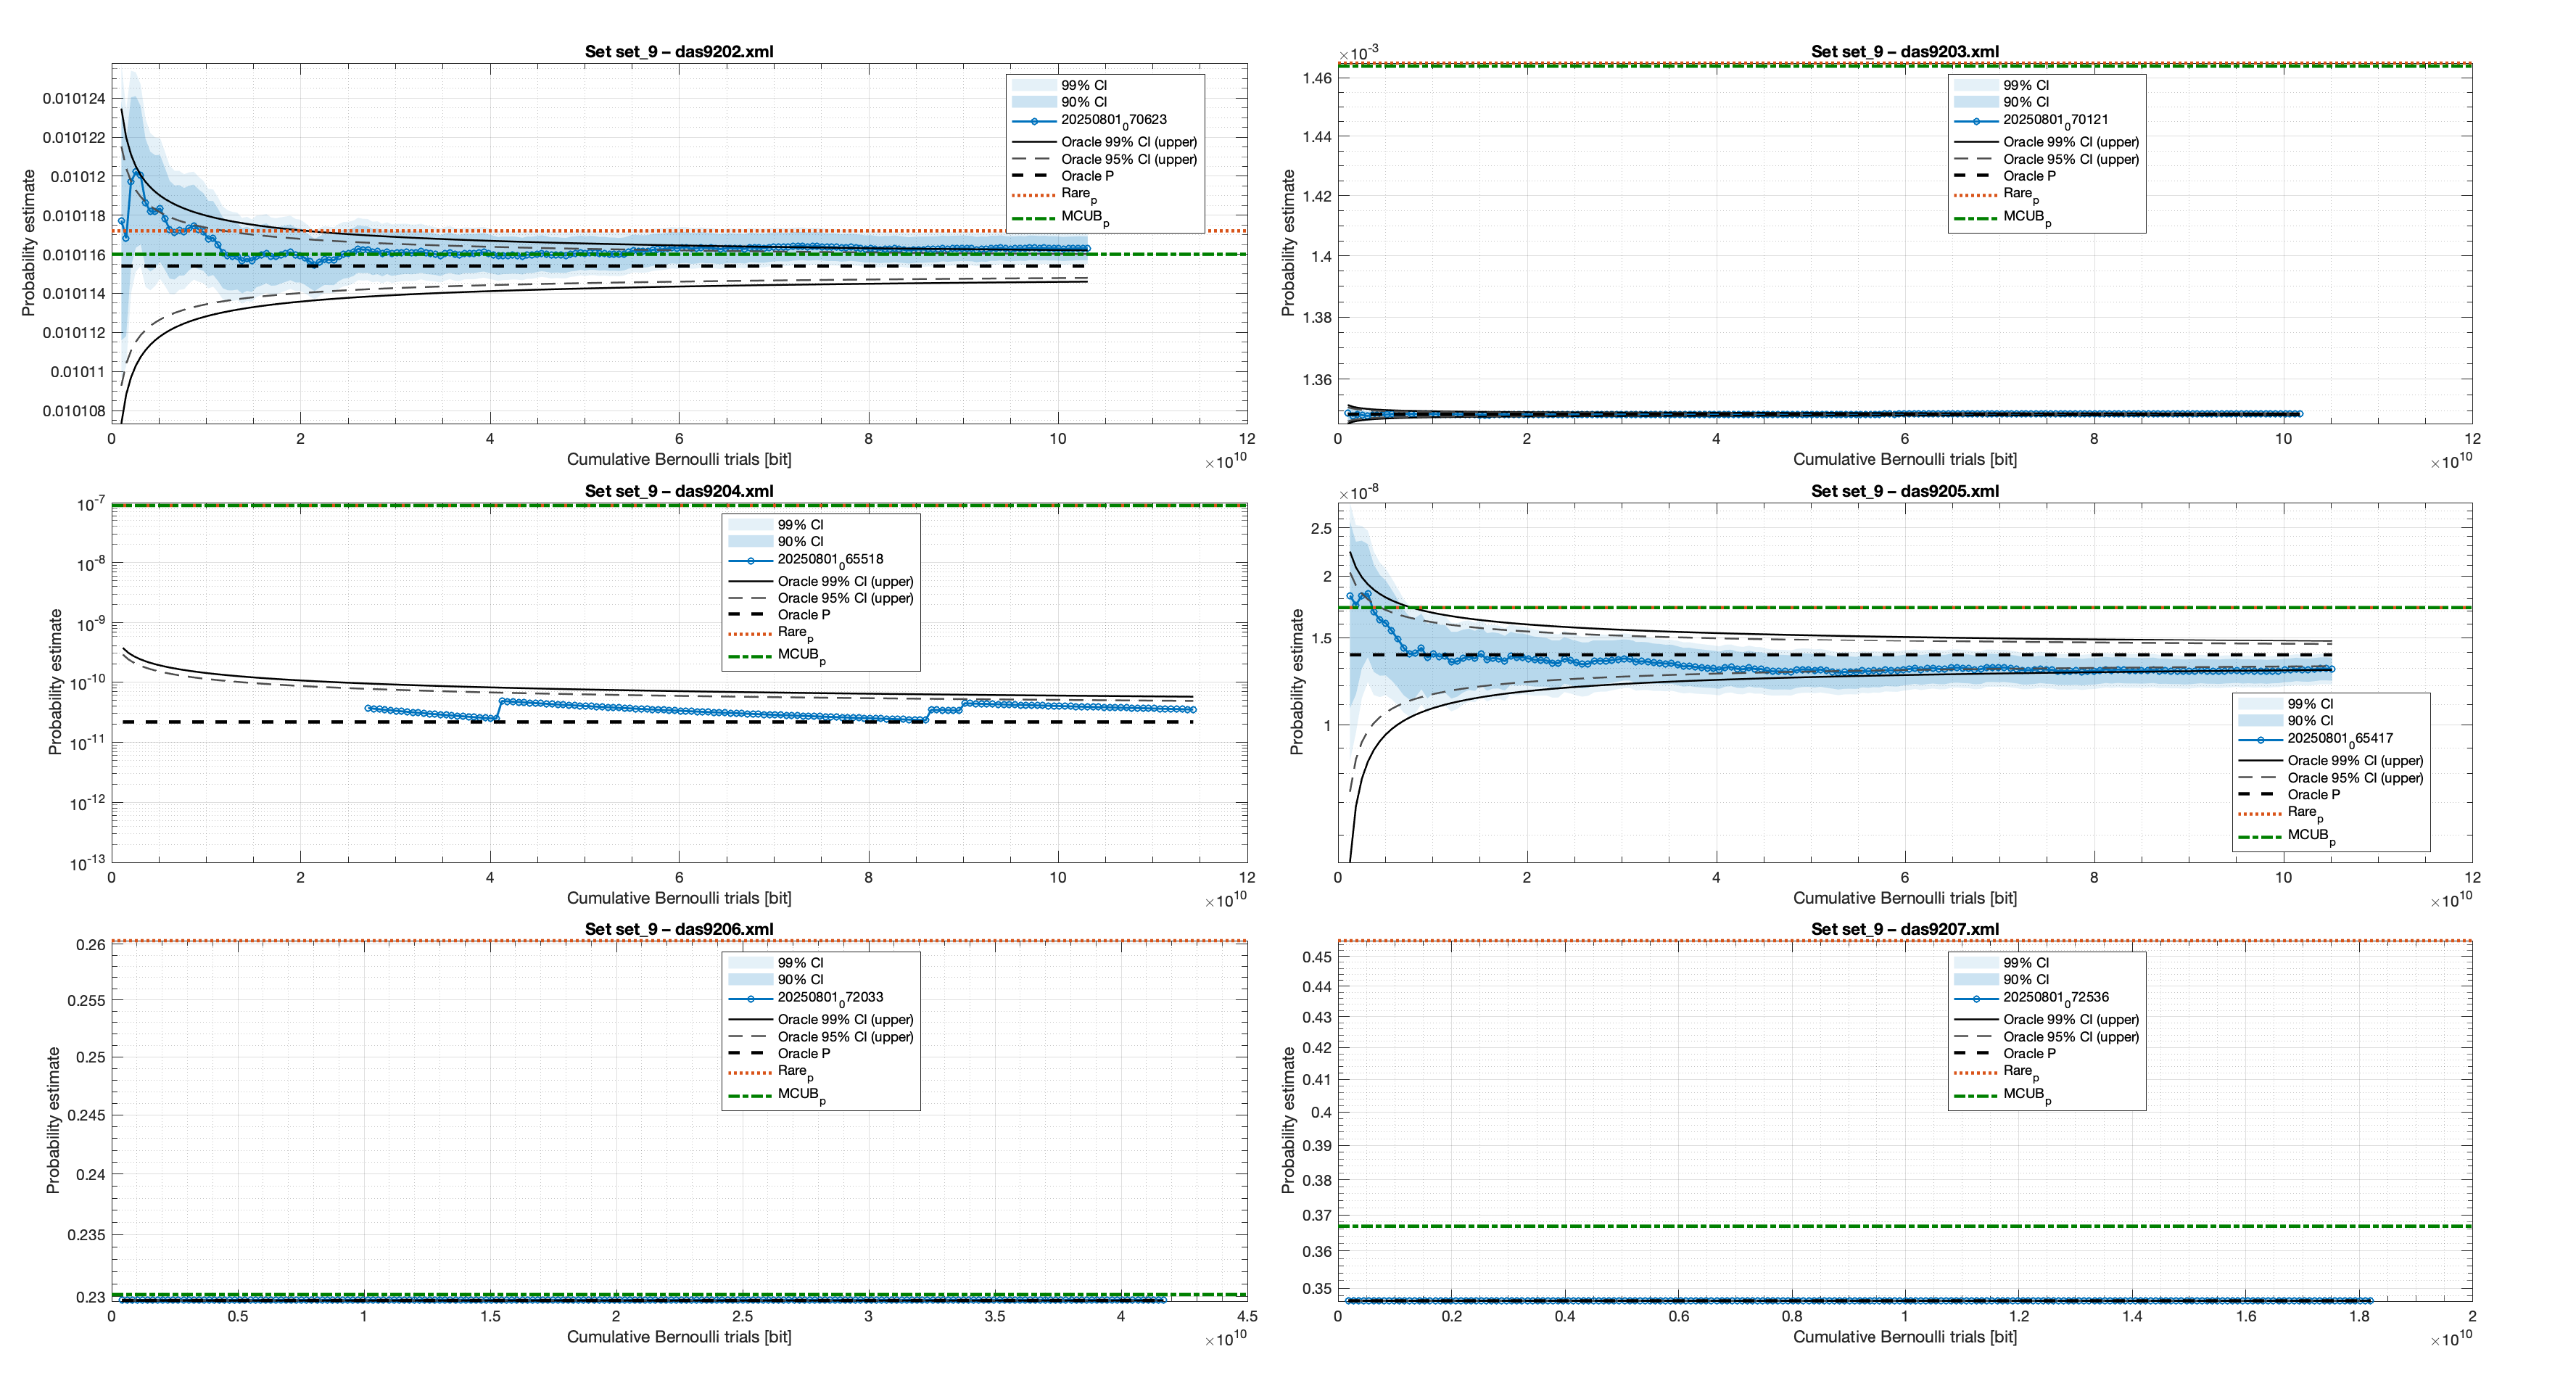
\includegraphics[height=1\textheight]{4_casestudy/conv_figeps.eps}
    \label{fig:convergence_run_01}
\end{figure}
\end{frame}

\subsection{Convergence Run -- Rare Event, Comparison with MCUB}
\begin{frame}
\begin{figure}[p]
    \centering
    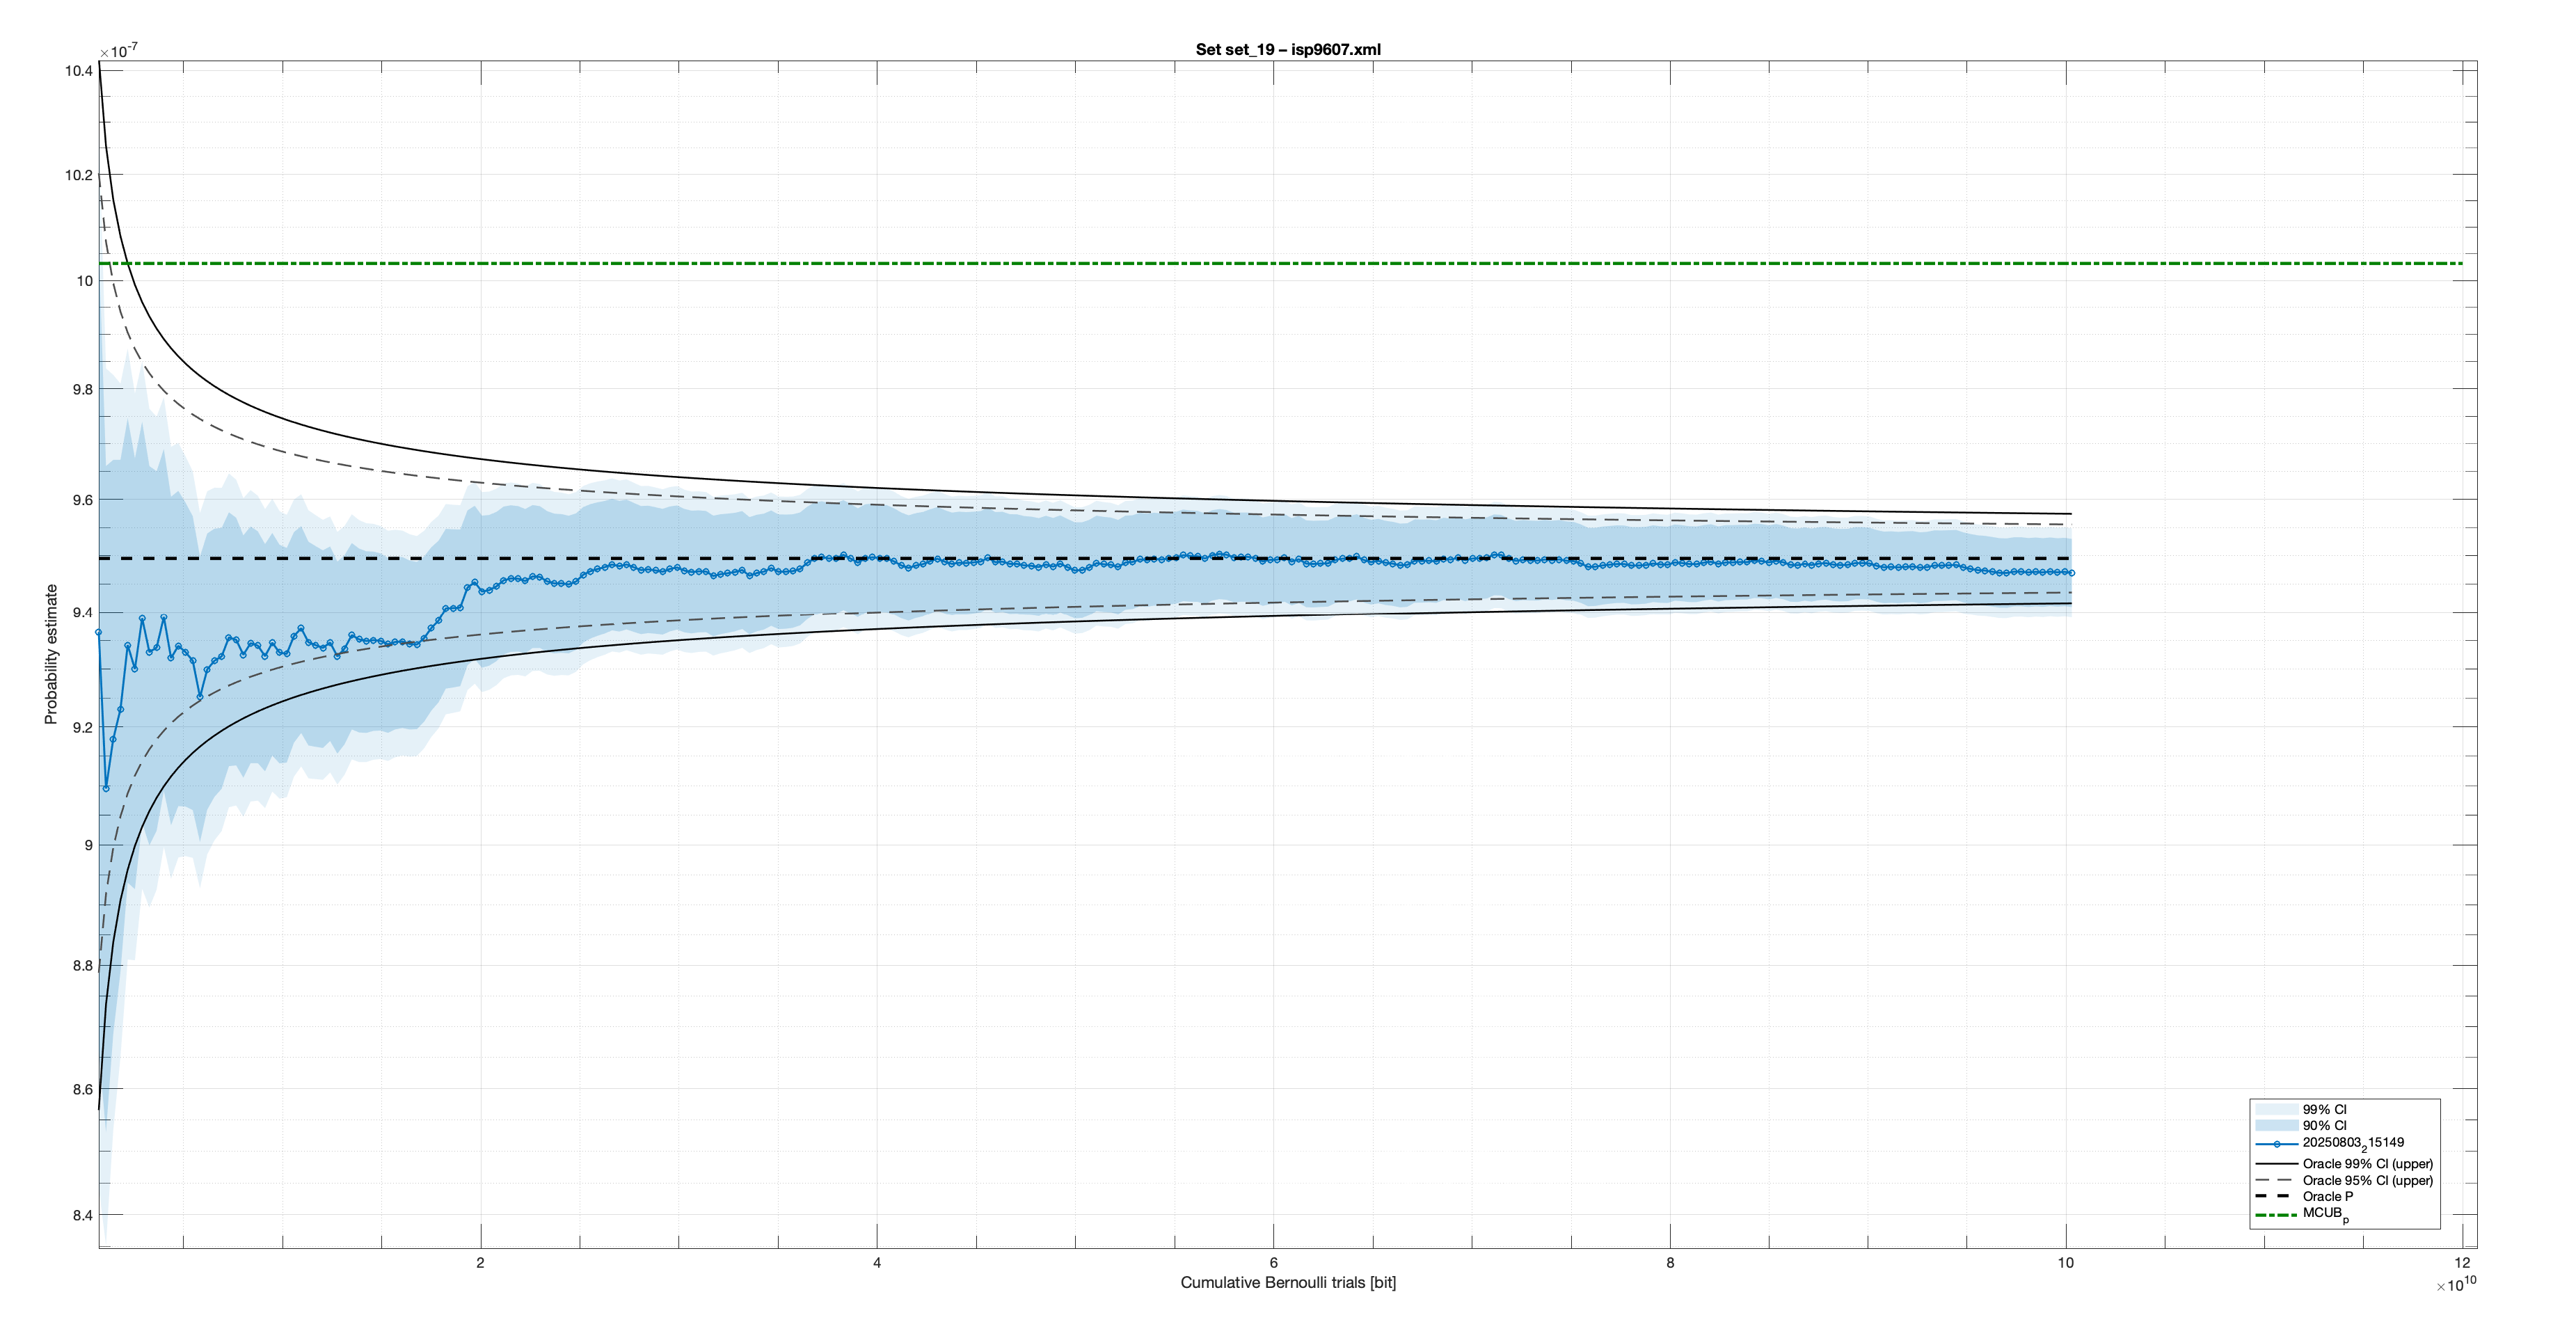
\includegraphics[height=0.9\textheight]{4_casestudy/conv_ips9607.eps}
    \label{fig:convergence_run_01}
\end{figure}
\end{frame}

\subsection{Convergence Free Run}
\begin{frame}
    \begin{figure}[h]
    \centering
    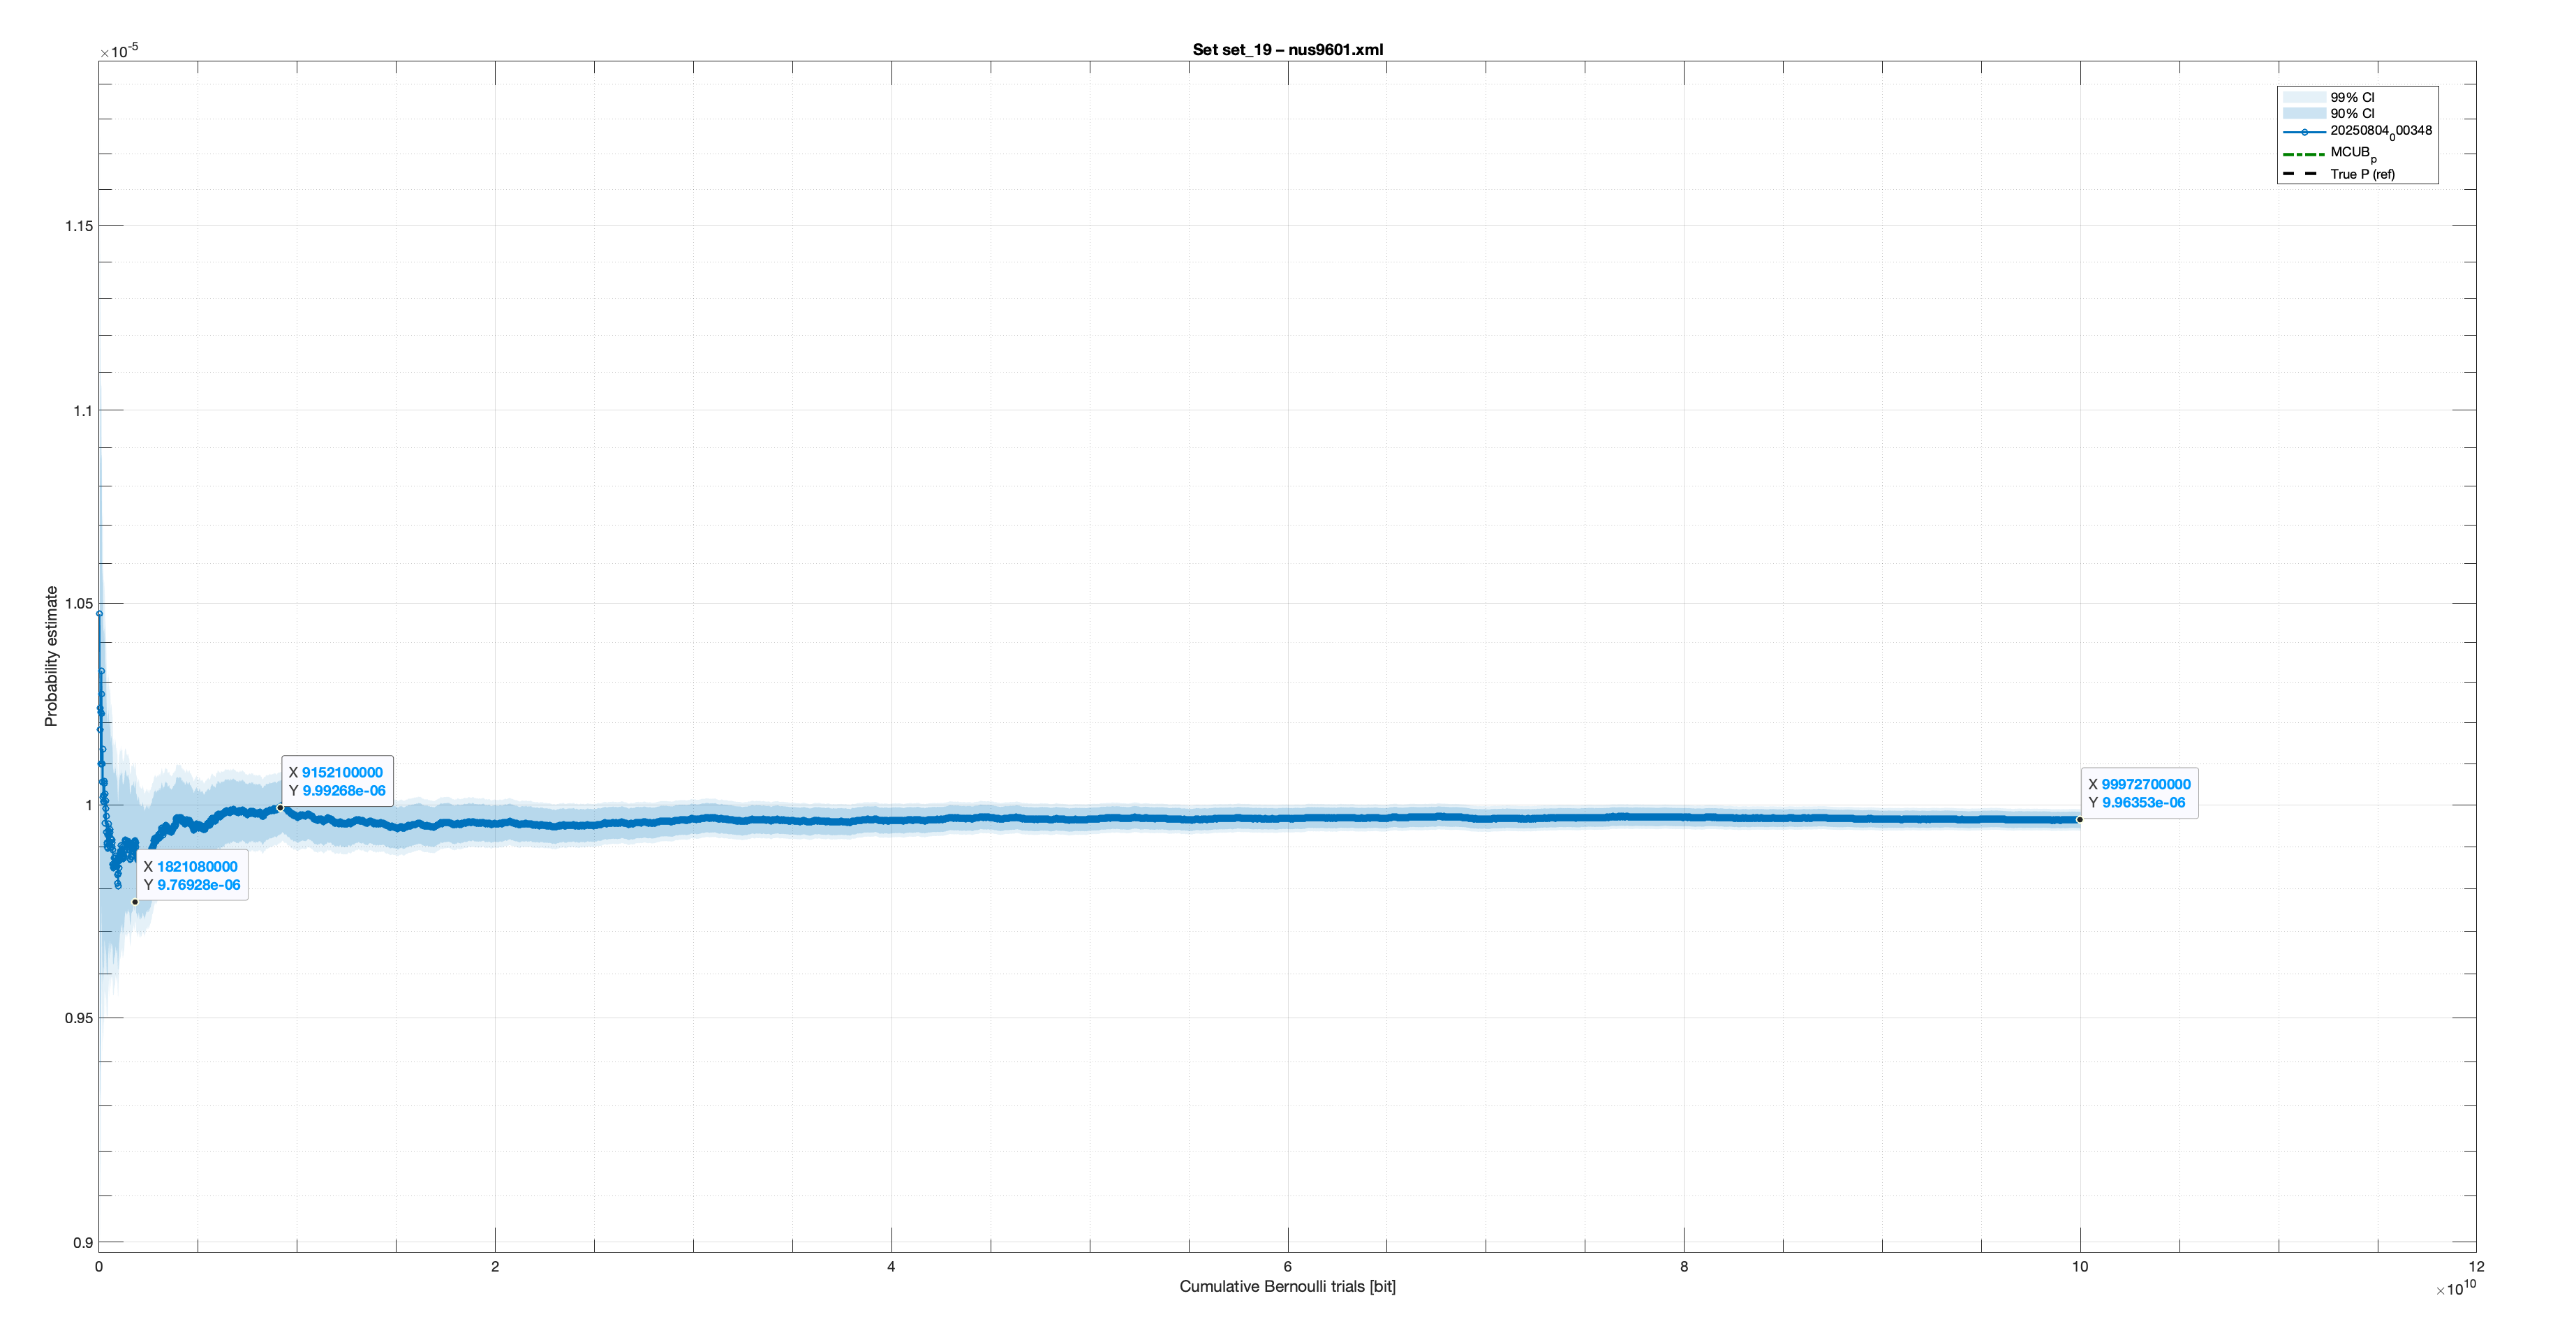
\includegraphics[width=1\textwidth]{4_casestudy/conv_nus9601.eps}
    \label{fig:rare}
\end{figure}
\end{frame}


\subsection{Aralia Fault Tree Data Set - Convergence for Rare Events}
\begin{frame}
    \input{4_casestudy/4_mae}
\end{frame}

% \subsection{Aralia Fault Tree Data Set - Throughput Benchmarks}
% \begin{frame}
%     \begin{figure}[h]
%     \centering
%     \includegraphics[width=0.9\textwidth]{4_casestudy/throughput/slides_nodes_vs_throughput.eps}
%     \caption{PDAG Node Count vs Throughput [bit/s]}
%     \label{fig:nodes_vs_throughput}
% \end{figure}
% \end{frame}




% \begin{frame}{Aralia Fault Tree Dataset}
% show the input dataset table\\
% \end{frame}

% \subsection{Results}
% \begin{frame}{Mar}
% show the input dataset table\\
% \end{frame}
% With the objective of bridging the gap between PDAG and probabilistic circuits, generate a section, including multiple frames, that (1) introduce the concept of the triplet definition of risk, (2) scenario modeling in PRA,  (3) event trees, (4) fault trees, (5) event tree / fault tree linking (together as a PRA model), (6) the concept of a PDAG, (7) PRA model as a PDAG. So, include at-least 7 frames, but you can use more. Include equations and definitions where appropriate.

\section{Research Objective 1: Bridge PRA Modeling Semantics with Probabilistic Circuits}
\begin{frame}
    \Large{\centerline{\textbf{Research Objective 1}}}
    \vspace{6pt}
    \large{\centerline{\textbf{Bridge PRA Modeling Semantics with Probabilistic Circuits}}}
\end{frame}

\subsection{PRA Overview}
\begin{frame}[allowframebreaks]
\frametitle{The Triplet Definition of Risk}
\begin{itemize}
  \item Define risk as a set of triplets, each representing:
    \begin{enumerate}
      \item What can go wrong? (\(S_i\))
      \item How likely is it to happen? (\(L_i\))
      \item What are the consequences? (\(X_i\))
    \end{enumerate}
        \vspace{6pt}
  \item
    \begin{equation}
    \label{eq:risk_triplets_slides}
      R \;=\;\bigl\{\langle S_i,\,L_i,\,X_i\rangle\bigr\}_{c},
    \end{equation}
    \(\,c\) represents completeness in enumerating \emph{all} relevant scenarios.
\end{itemize}
\end{frame}

\begin{frame}[allowframebreaks]
\frametitle{Scenario \(S_i\) Modeling in PRA}
\begin{itemize}
  \item Each scenario unfolds from initiating events (IEs), followed by conditional branching events.
          \vspace{6pt}
  \item Fundamental goal: assign probabilities to these scenarios {and} assess resulting outcomes (e.g., core damage, large release).
          \vspace{6pt}
  \item Implementation typically uses structured diagrams such as:
    \begin{itemize}
      \item Event Trees (ETs): forward chaining from IE to various end states.
      \item Fault Trees (FTs): top-down decomposition to basic events (component failures).
    \end{itemize}
\end{itemize}
\end{frame}

\begin{frame}[t, allowframebreaks]
\frametitle{Event Trees}
\begin{figure}[ht!]
\centering
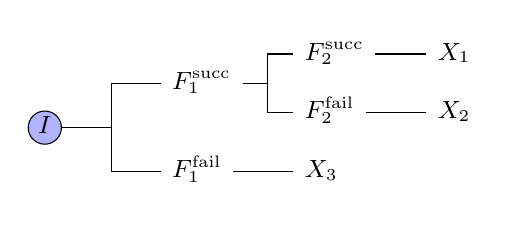
\begin{tikzpicture}
\tikzset{grow'=right,level distance=48pt}
\tikzset{execute at begin node=\strut}
\tikzset{every tree node/.style={anchor=base west}}
\tikzset{
    edge from parent/.append style={very thick},
    edge from parent/.style={
        draw,
        edge from parent path={
            (\tikzparentnode.east) -| ($(\tikzparentnode.east)!0.5!(\tikzchildnode.west)$) |- (\tikzchildnode.west)
        },
    },
    every node/.style={anchor=center,font=\small\bfseries, text centered, inner sep=0pt},
    every level 0 node/.style={circle, font=\small\bfseries, draw, fill=blue!30, inner sep=0pt},
    every internal node/.style={font=\small, inner sep=4pt},
    every leaf node/.style={rectangle, draw, fill=blue!30, minimum width=2.5cm, text centered},
    frontier/.style={distance from root=400pt},
}
\Tree [.\(I\)
    [.\(F_1^{\text{succ}}\)
        [.\(F_2^{\text{succ}}\)
            [.\(X_1\) ]
        ]
        [.\(F_2^{\text{fail}}\)
            [.\(X_2\) ]
        ]
    ]
    [.\(F_1^{\text{fail}}\)
        [.\(X_3\) ]
    ]
]
\end{tikzpicture}
\caption{Illustrative event tree with an initiating event \(I\), two functional events \(F_1\) and \(F_2\), and three end-states \(X_1, X_2, X_3\).}
\label{fig:event_tree_example}
\end{figure}
\begin{itemize}
  \item An Event Tree represents how an initiating event \(I\) can branch into multiple functional-event outcomes.
  \item Each functional event \(F_k\) may succeed or fail, driving the path toward a distinct end-state \(X_j\).  
  \item If \(\omega_j\) denotes one branch leading to \(X_j\), then the branch probability often factors as 
    \[
      p(\omega_j) \;=\; p(I)\;\times\;\prod_{k=1}^{n} \; p\bigl(F_k^{\alpha_k} \;\mid\; \text{all previous outcomes}\bigr).
    \]
  \item As a logical expression, each \(\omega_j\) translates to an AND of success/failure literals, and the overall set of end-states is an OR of these branches:
    \[
      \Omega \;=\;\omega_1 \;\lor\;\omega_2 \;\lor\;\dots\;\lor\;\omega_m.
    \]
  \item Consequently, ETs are in \emph{sum of products} (SOP) or \emph{disjunctive normal form} (DNF), where each product term identifies one success/failure path and the scenario-level outcome is the logical OR across all such paths.
  \vspace{4pt}
  \item Graphically straightforward, but can combinatorially expand for deep branching.
\end{itemize}
\end{frame}

\begin{frame}[t, allowframebreaks]
\frametitle{Fault Trees}
    \begin{figure}[h]
    \centering
    \includegraphics[width=0.5\textwidth]{1_concepts/ft.png}
    \caption{Fault tree with 6 basic events, top event $X = (a_1\bigwedge b_1) \bigvee (a_2\bigwedge b_2) \bigvee (a_3\bigwedge b_3)$}
    \label{fig:ft}
\end{figure}
\begin{itemize}
  \item A Fault Tree describes how a top event (system failure) can result from lower-level component or subsystem failures.
  \item Internal gates (AND, OR, \(k\)-of-\(n\), etc.) combine events in logical fashion:
    \[
      \text{Output} \;=\;
      \begin{cases}
         \bigwedge_{i=1}^k e_i, & \text{(AND)}\\
         \bigvee_{i=1}^k e_i, & \text{(OR)}\\
         \dots
      \end{cases}
    \]
  \item Basic events (BEs) in the leaves have assigned probabilities \(p(b)\).  Independence often assumed unless modeling common-cause failures.
  \item The top event failure probability can be written as:
    \begin{equation}
    \label{eq:top_event_probability_slides}
    \Pr[\text{Top Fail}] \;=\; \sum_{S \subseteq \,\mathcal{B}} 
      \Bigl[
        \pi_{F}(S, \text{Top}) 
        \prod_{b\in S} p(b)\prod_{b\notin S}[1 - p(b)]
      \Bigr].
    \end{equation}
\end{itemize}
\end{frame}

\begin{frame}[t, allowframebreaks]
\frametitle{Linking Event Trees and Fault Trees in PRA}
\begin{itemize}
  \item Real systems often combine:
    \begin{itemize}
      \item Forward branching dynamics via Event Trees (ET).
      \item Subsystem or component reliability logic via Fault Trees (FT).
    \end{itemize}
  \item An event tree branch may call a specific FT top event to collect system failure or success.
  \item Conversely, a fault tree output may feed back into an event tree branch as an initiating event or functional node outcome.
  \item This multi-level interconnection \(\implies\) a need for a unified model capturing both forward branching (ET) and hierarchical failure logic (FT).
\end{itemize}
\end{frame}

\begin{frame}[t, allowframebreaks]
\frametitle{Probabilistic Directed Acyclic Graph (PDAG)}
\begin{itemize}
  \item A PDAG is a Directed Acyclic Graph whose edges carry either:
    \begin{itemize}
      \item Conditional probabilities (e.g., for event tree branches).  
      \item Logical dependencies (e.g., for fault tree gates).
    \end{itemize}
  \item Nodes may include:
    \begin{itemize}
      \item Basic events (BEs) with known probabilities.
      \item ET or FT intermediate events storing partial results.
      \item Any top-level node (e.g., a final end-state) with no children.
    \end{itemize}
  \item The absence of cycles guarantees consistent flow from initial seeds (basic events, initiating events) to final outcomes.
  \item PDAG forms the structural backbone for bridging scenario-based expansions with gate-based logic in a single coherent representation.
\end{itemize}
\end{frame}

\subsection{Probabilistic Circuits Overview}
\begin{frame}[t, allowframebreaks]
\frametitle{Probabilistic Circuits: A Brief Overview}
    \begin{figure}[h]
    \centering
    \includegraphics[height=0.5\textheight]{1_concepts/pc.png}
    \caption{Probabilistic circuit with 4 inputs $X_i$, product gates (blue), sum gate (orange)}
    \label{fig:pc}
\end{figure}
\end{frame}

\begin{frame}[t, allowframebreaks]
\begin{itemize}
  \item A \textbf{probabilistic circuit} is a directed acyclic graph (DAG) that encodes a joint probability distribution through \emph{sum-gates} and \emph{product-gates}.
  \item \textbf{Sum-gates} approximate mixture distributions:
    \[
      p_v(\mathbf{x})
      \;=\;
      \sum_{u\in \operatorname{ch}(v)} \theta_{v,u}\,p_u(\mathbf{x}),
      \quad
      \text{with }
      \sum_{u\in \operatorname{ch}(v)} \theta_{v,u} = 1.
    \]
    Each child distribution is weighted by a nonnegative parameter \(\theta_{v,u}\).
  \item \textbf{Product-gates} factorize independent variable sets:
    \[
      p_v(\mathbf{x})
      \;=\;
      \prod_{u\in \operatorname{ch}(v)} p_u\bigl(\mathbf{x}_{u}\bigr),
    \]
    assuming disjoint subsets of variables for each child \(u\).
  \item \textbf{Leaf nodes} (inputs) often correspond to known base distributions. When evaluated upward through the DAG, each internal node yields its own distribution, culminating in a root node that represents the full model.
  \item \textbf{Key motivation}:
    \begin{itemize}
      \item Tractable inference: evaluation and certain marginal or conditional queries can be performed in time proportional to circuit size.  
      \item Decomposability and modularity: separate, interpretable substructures that can be reused or combined for large-scale systems.
    \end{itemize}
\end{itemize}
\end{frame}

\subsection{PRA PDAGs to Probabilistic Circuits}
\begin{frame}[allowframebreaks]
\frametitle{Compiled PRA Graphs are PDAGs}
\begin{itemize}
  \item A unified PRA model can be viewed as
    \[
      \mathcal{M} 
      \;=\;
      \langle 
        \mathcal{V},\,\mathcal{A},\, \{p(b)\},\, \{\theta_{u\to v}\},\,\pi_{F}
      \rangle,
    \]
    where \(\mathcal{V}\) includes basic events, ET nodes, and FT gates, and \(\mathcal{A}\) is the acyclic edge set.
  \item Event-tree edges carry transitional probabilities \(\theta_{u\to v}\) summing to 1 from each node.
  \item Fault-tree nodes embed Boolean logic \(\pi_F\) that checks if inputs fail under a subset of basic events.
  \framebreak
  \item This PDAG perspective:
    \begin{itemize}
      \item Ensures systematic accounting of all scenario paths and subsystem logic.
      \item Aligns naturally with tractable Probabilistic Circuits, since each node’s distribution/function can be embedded in a sum-product style DAG.
      \item Offers a foundation for efficient Monte Carlo or advanced inference methods.
    \end{itemize}
    \vspace{6pt}
    \item Ongoing work to bridge PRA PDAG semantics with Probabilistic Circuits:
    \begin{itemize}
      \item PDAGs can be transformed to equivalent canonical forms (there are tradeoffs).
    \end{itemize}
\end{itemize}
\end{frame}
% % !TeX TS-program = lualatex
%----------------------------------------------------------------------------------------
%    PACKAGES AND THEMES
%----------------------------------------------------------------------------------------

\documentclass[aspectratio=169,xcolor=dvipsnames]{beamer}
\usetheme{SimpleDarkBlue}

\usepackage{booktabs}  % professionally typeset tables
\usepackage{amsmath}
\usepackage{amsthm}
\usepackage{amssymb} 
\usepackage{amsfonts}
\usepackage{tikz}
\usepackage{tikz-qtree}
\usetikzlibrary{calc,positioning}
\usepackage{pgfpages}
% \setbeameroption{show notes on second screen}

\usepackage{textcomp}  % better copyright sign, among other things
\usepackage{lipsum}    % filler text
\usepackage{lscape}
\usepackage{longtable}
\usepackage{siunitx}
% Please add the following required packages to your document preamble:
\usepackage{multirow}
\usepackage[table,xcdraw]{xcolor}
\usepackage{xstring}
\usepackage{relsize}
\usepackage{hyperref}
\usepackage{graphicx} % Allows including images
\usepackage{fontspec}
%\usepackage{helvet}
\setsansfont{Open Sans}
%----------------------------------------------------------------------------------------
%    TITLE PAGE
%----------------------------------------------------------------------------------------

\title{A Data-Parallel Monte Carlo Framework for Large-Scale PRA
using Probabilistic Circuits}
\subtitle{Preliminary Exam}

\author{Arjun Earthperson}

\institute
{
    Department of Nuclear Engineering \\
    North Carolina State University % Your institution for the title page
}
\date{March 6, 2025} % Date, can be changed to a custom date

%----------------------------------------------------------------------------------------
%    PRESENTATION SLIDES
%----------------------------------------------------------------------------------------

\begin{document}
% \hypersetup{
% 	pdfkeywords={SP-Right}
% }
\begin{frame}
    % Print the title page as the first slide
    \titlepage
\end{frame}


% \begin{frame}{Overview}
%     % Throughout your presentation, if you choose to use \section{} and \subsection{} commands, these will automatically be printed on this slide as an overview of your presentation
%     \tableofcontents
% \end{frame}


% \begin{frame}{Acknowledgments}
% Funding for this research has come from ...\\
% I would like to thank ...
% \end{frame}

\section*{About Me}
\begin{frame}[t]
\textbf{Education}
\vspace{2pt}
{\smaller[1]
\begin{itemize}
\setlength{\baselineskip}{2pt}
    \item {
    \textbf{MS, Nuclear Engineering}, North Carolina State University (2023)\\
    {{\smaller[1.2]Thesis: \color{red600}{"Integrating Dual Error Propagation into Dynamic Event Trees to Support Fission Battery Probabilistic Risk Assessments"}}}
    }
    \vspace{4pt}
    \item {\textbf{BS, Electrical Engineering}, University of California, Los Angeles (2017)\\
    {{\smaller[1.2]Capstone: \color{red600}{"Integer Hardware Optimizations on TI-C6000 DSPs for Low-Power IoT Applications"}}}
    }
\end{itemize}
}
\vspace{8pt}
\textbf{Work Experience}
{\smaller[1]
\begin{itemize}
\setlength{\baselineskip}{2pt}
    \item{\textbf{Intern}, Idaho National Laboratory (Summer 2021)\\
        {{\smaller[1.2]Project: \color{red600}{Coupled OpenPRA's OpenEPL engine with EMRALD.}}}
    }
    \vspace{2pt}
    \item{\textbf{Programmer}, The B. John Garrick Institute for the Risk Sciences, UCLA (2018--2020)\\
    {{\smaller[1.2]\color{red600}{Developed the Hybrid Causal Logic and Phoenix human reliability assessment web applications.}}}
    }
\end{itemize}
}
\vspace{8pt}
\textbf{Awards}
{\smaller[1]
\begin{itemize}
    \item{\textbf{1\textsuperscript{st} Place Graduate Student Winner}, ASME SERAD Student Safety Innovation Challenge (2023)\\
    {{\smaller[1.2]Paper: \color{red600}{Introducing OpenPRA: A Web-Based Framework for Collaborative Probabilistic Risk Assessment}}}
    }
\end{itemize}
} 
\end{frame}
% \setlength{\bibhang}{4pt} % no indentation


\subsection*{Research Contributions}
\begin{frame}[t,allowframebreaks]

\nocite{*}
\hspace{-8pt}\textbf{Software}
\vspace{2pt}
\printbibliography[type=misc, resetnumbers=false]
\vspace{4pt}

\vspace{4pt}
\hspace{-8pt}\textbf{Journal Articles}
\vspace{2pt}
\printbibliography[type=article, resetnumbers=true]
\vspace{4pt}

\hspace{-8pt}\textbf{Conference Papers}
\vspace{2pt}
\printbibliography[type=inproceedings, resetnumbers=true]

\end{frame}


% Overview slide removed; high-level story arc slide added instead.
% One-slide “North-Star” story arc
\begin{frame}[t]{Research Story in One Slide}
  \begin{enumerate}[<+->]
    \item \textbf{Problem.}  Exact PRA quantification crumbles beyond a few hundred gates; industry still waits hours–days for large models.
    \item \textbf{Idea.}  Treat the \emph{entire} PRA—event trees \& fault trees—as one probabilistic DAG and evaluate it via massively–parallel Monte-Carlo.
    \item \textbf{Enablers.}  Hardware-native voting gates, a Monte-Carlo–oriented compilation pipeline, and GPU-resident bit-packed kernels.
    \item \textbf{Evidence.}  186× compile-time reduction; sub-percent error on $\sim10^3$-event graphs in <5 s on a laptop GPU.
    \item \textbf{Impact.}  Opens path to real-time, high-fidelity risk insights and lays groundwork for dynamic \& correlated extensions.
  \end{enumerate}
\end{frame}

\title{A Data-Parallel Monte Carlo Framework for Large-Scale PRA
using Probabilistic Circuits}
\subtitle{PhD Defense, Nuclear PRA}

\section{Motivation}
\subsection{PRA Unmet Needs}
\begin{frame}[t]{Long-Standing Needs in PRA Quantification}
  \begin{itemize}
    \item Large-scale PRA models ($\geq\space\approx10^4$ components) remain computationally taxing.
    \item To ease burden, approximations are used, implicating accuracy.
    \item No knobs for controlling trade-off between accuracy and speed.
  \end{itemize}
\end{frame}

\begin{frame}[t]{Long-Standing Needs in PRA Quantification}
  \begin{itemize}
    \item Large-scale PRA models ($\geq\space\approx10^4$ components) remain computationally taxing.
    \item To ease burden, approximations are used, implicating accuracy.
    \item No knobs for controlling trade-off between accuracy and speed.
  \end{itemize}
    \vspace{16pt}
    Large-scale PRA models still takes days to quantify.
\end{frame}

\subsection{Emerging Opportunities}
\begin{frame}[t]{Evolving Hardware Landscape}
\textbf{Industry responding to emerging ML compute challenges by investing heavily in data-parallel hardware}
  \begin{itemize} 
    \item GPUs, tensor cores provide high throughput for integer operations.
    \item Current-gen consumer hardware already supports specialized ops (Intel AMX, VNNI).
  \end{itemize}
  \vspace{8pt}
\textbf{Designed for Massive Workloads}
  \begin{itemize} 
    \item $\approx10^9$ parameters on mobile devices, $\approx10^{12}$ on HPC/cloud.
    \item Comparatively, largest PRA models: $\approx10^6$ parameters.
  \end{itemize}
\end{frame}

\begin{frame}[t]{Evolving Hardware Landscape}
\textbf{Industry responding to emerging ML compute challenges by investing heavily in data-parallel hardware}
  \begin{itemize} 
    \item GPUs, tensor cores provide high throughput for integer operations.
    \item Current-gen consumer hardware already supports specialized ops (Intel AMX, VNNI).
  \end{itemize}
  \vspace{8pt}
\textbf{Designed for Massive Workloads}
  \begin{itemize} 
    \item $\approx10^9$ parameters on mobile devices, $\approx10^{12}$ on HPC/cloud.
    \item Comparatively, largest PRA models: $\approx10^6$ parameters.
  \end{itemize}
      \vspace{12pt}
  \textit{But PRA models have no overlap with ML models.}\\
\end{frame}

\begin{frame}[t]{Evolving Hardware Landscape}
\textbf{Industry responding to emerging ML compute challenges by investing heavily in data-parallel hardware}
  \begin{itemize} 
    \item GPUs, tensor cores provide high throughput for integer operations.
    \item Current-gen consumer hardware already supports specialized ops (Intel AMX, VNNI).
  \end{itemize}
  \vspace{8pt}
\textbf{Designed for Massive Workloads}
  \begin{itemize} 
    \item $\approx10^9$ parameters on mobile devices, $\approx10^{12}$ on HPC/cloud.
    \item Comparatively, largest PRA models: $\approx10^6$ parameters.
  \end{itemize}
      \vspace{12pt}
  \textit{But PRA models have no overlap with ML models(?)}\\
\end{frame}

\begin{frame}[t]{Evolving Hardware Landscape}
\textbf{Industry responding to emerging ML compute challenges by investing heavily in data-parallel hardware}
  \begin{itemize} 
    \item GPUs, tensor cores provide high throughput for integer operations.
    \item Current-gen consumer hardware already supports specialized ops (Intel AMX, VNNI).
  \end{itemize}
  \vspace{8pt}
\textbf{Designed for Massive Workloads}
  \begin{itemize} 
    \item $\approx10^9$ parameters on mobile devices, $\approx10^{12}$ on HPC/cloud.
    \item Comparatively, largest PRA models: $\approx10^6 \text{ to } 10^9$ parameters.
  \end{itemize}
    \vspace{12pt}
\textit{But PRA models have no overlap with ML models (?)} - \textbf{Research Question}\\
\textit{Probability estimation analogous to inference in feed-forward networks.}
\end{frame}

\note{
    \begin{itemize}
        \item here, I want to say that hardware vendors, and the industry in general is responding to emerging AI/ML compute challenges by investing heavily in data-parallel hardware (GPGPU, ASIC accelerators, tensor processors). Ops/W/die is improving, opening up opportunities on HPC/cloud as well edge/personal devices. At the same time, the sheer complexity of AI/ML models is many orders of magnitude (trillions of params) larger vs PRA models (currently hundreds of thousands to millions of params). If the algorithms could leverage the appropriate hardware, PRA quantification (in terms of size) would have been solved by now. But, SOTA PRA methods are nowhere close to being able to leverage this new/emerging hardware. We need new methods.
    \end{itemize}
}

%% 

\input{0_intro/5_research_contrib/1_questions}
\input{0_intro/5_research_contrib/2_contrib_overview}
% With the objective of bridging the gap between PDAG and probabilistic circuits, generate a section, including multiple frames, that (1) introduce the concept of the triplet definition of risk, (2) scenario modeling in PRA,  (3) event trees, (4) fault trees, (5) event tree / fault tree linking (together as a PRA model), (6) the concept of a PDAG, (7) PRA model as a PDAG. So, include at-least 7 frames, but you can use more. Include equations and definitions where appropriate.

\section{Research Objective 1: Bridge PRA Modeling Semantics with Probabilistic Circuits}
\begin{frame}
    \Large{\centerline{\textbf{Research Objective 1}}}
    \vspace{6pt}
    \large{\centerline{\textbf{Bridge PRA Modeling Semantics with Probabilistic Circuits}}}
\end{frame}

\subsection{PRA Overview}
\begin{frame}[allowframebreaks]
\frametitle{The Triplet Definition of Risk}
\begin{itemize}
  \item Define risk as a set of triplets, each representing:
    \begin{enumerate}
      \item What can go wrong? (\(S_i\))
      \item How likely is it to happen? (\(L_i\))
      \item What are the consequences? (\(X_i\))
    \end{enumerate}
        \vspace{6pt}
  \item
    \begin{equation}
    \label{eq:risk_triplets_slides}
      R \;=\;\bigl\{\langle S_i,\,L_i,\,X_i\rangle\bigr\}_{c},
    \end{equation}
    \(\,c\) represents completeness in enumerating \emph{all} relevant scenarios.
\end{itemize}
\end{frame}

\begin{frame}[allowframebreaks]
\frametitle{Scenario \(S_i\) Modeling in PRA}
\begin{itemize}
  \item Each scenario unfolds from initiating events (IEs), followed by conditional branching events.
          \vspace{6pt}
  \item Fundamental goal: assign probabilities to these scenarios {and} assess resulting outcomes (e.g., core damage, large release).
          \vspace{6pt}
  \item Implementation typically uses structured diagrams such as:
    \begin{itemize}
      \item Event Trees (ETs): forward chaining from IE to various end states.
      \item Fault Trees (FTs): top-down decomposition to basic events (component failures).
    \end{itemize}
\end{itemize}
\end{frame}

\begin{frame}[t, allowframebreaks]
\frametitle{Event Trees}
\begin{figure}[ht!]
\centering
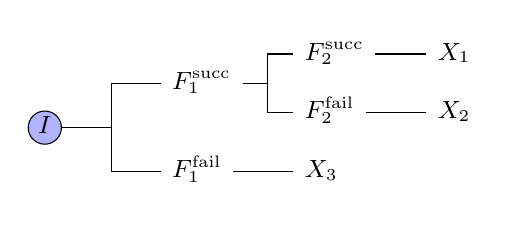
\begin{tikzpicture}
\tikzset{grow'=right,level distance=48pt}
\tikzset{execute at begin node=\strut}
\tikzset{every tree node/.style={anchor=base west}}
\tikzset{
    edge from parent/.append style={very thick},
    edge from parent/.style={
        draw,
        edge from parent path={
            (\tikzparentnode.east) -| ($(\tikzparentnode.east)!0.5!(\tikzchildnode.west)$) |- (\tikzchildnode.west)
        },
    },
    every node/.style={anchor=center,font=\small\bfseries, text centered, inner sep=0pt},
    every level 0 node/.style={circle, font=\small\bfseries, draw, fill=blue!30, inner sep=0pt},
    every internal node/.style={font=\small, inner sep=4pt},
    every leaf node/.style={rectangle, draw, fill=blue!30, minimum width=2.5cm, text centered},
    frontier/.style={distance from root=400pt},
}
\Tree [.\(I\)
    [.\(F_1^{\text{succ}}\)
        [.\(F_2^{\text{succ}}\)
            [.\(X_1\) ]
        ]
        [.\(F_2^{\text{fail}}\)
            [.\(X_2\) ]
        ]
    ]
    [.\(F_1^{\text{fail}}\)
        [.\(X_3\) ]
    ]
]
\end{tikzpicture}
\caption{Illustrative event tree with an initiating event \(I\), two functional events \(F_1\) and \(F_2\), and three end-states \(X_1, X_2, X_3\).}
\label{fig:event_tree_example}
\end{figure}
\begin{itemize}
  \item An Event Tree represents how an initiating event \(I\) can branch into multiple functional-event outcomes.
  \item Each functional event \(F_k\) may succeed or fail, driving the path toward a distinct end-state \(X_j\).  
  \item If \(\omega_j\) denotes one branch leading to \(X_j\), then the branch probability often factors as 
    \[
      p(\omega_j) \;=\; p(I)\;\times\;\prod_{k=1}^{n} \; p\bigl(F_k^{\alpha_k} \;\mid\; \text{all previous outcomes}\bigr).
    \]
  \item As a logical expression, each \(\omega_j\) translates to an AND of success/failure literals, and the overall set of end-states is an OR of these branches:
    \[
      \Omega \;=\;\omega_1 \;\lor\;\omega_2 \;\lor\;\dots\;\lor\;\omega_m.
    \]
  \item Consequently, ETs are in \emph{sum of products} (SOP) or \emph{disjunctive normal form} (DNF), where each product term identifies one success/failure path and the scenario-level outcome is the logical OR across all such paths.
  \vspace{4pt}
  \item Graphically straightforward, but can combinatorially expand for deep branching.
\end{itemize}
\end{frame}

\begin{frame}[t, allowframebreaks]
\frametitle{Fault Trees}
    \begin{figure}[h]
    \centering
    \includegraphics[width=0.5\textwidth]{1_concepts/ft.png}
    \caption{Fault tree with 6 basic events, top event $X = (a_1\bigwedge b_1) \bigvee (a_2\bigwedge b_2) \bigvee (a_3\bigwedge b_3)$}
    \label{fig:ft}
\end{figure}
\begin{itemize}
  \item A Fault Tree describes how a top event (system failure) can result from lower-level component or subsystem failures.
  \item Internal gates (AND, OR, \(k\)-of-\(n\), etc.) combine events in logical fashion:
    \[
      \text{Output} \;=\;
      \begin{cases}
         \bigwedge_{i=1}^k e_i, & \text{(AND)}\\
         \bigvee_{i=1}^k e_i, & \text{(OR)}\\
         \dots
      \end{cases}
    \]
  \item Basic events (BEs) in the leaves have assigned probabilities \(p(b)\).  Independence often assumed unless modeling common-cause failures.
  \item The top event failure probability can be written as:
    \begin{equation}
    \label{eq:top_event_probability_slides}
    \Pr[\text{Top Fail}] \;=\; \sum_{S \subseteq \,\mathcal{B}} 
      \Bigl[
        \pi_{F}(S, \text{Top}) 
        \prod_{b\in S} p(b)\prod_{b\notin S}[1 - p(b)]
      \Bigr].
    \end{equation}
\end{itemize}
\end{frame}

\begin{frame}[t, allowframebreaks]
\frametitle{Linking Event Trees and Fault Trees in PRA}
\begin{itemize}
  \item Real systems often combine:
    \begin{itemize}
      \item Forward branching dynamics via Event Trees (ET).
      \item Subsystem or component reliability logic via Fault Trees (FT).
    \end{itemize}
  \item An event tree branch may call a specific FT top event to collect system failure or success.
  \item Conversely, a fault tree output may feed back into an event tree branch as an initiating event or functional node outcome.
  \item This multi-level interconnection \(\implies\) a need for a unified model capturing both forward branching (ET) and hierarchical failure logic (FT).
\end{itemize}
\end{frame}

\begin{frame}[t, allowframebreaks]
\frametitle{Probabilistic Directed Acyclic Graph (PDAG)}
\begin{itemize}
  \item A PDAG is a Directed Acyclic Graph whose edges carry either:
    \begin{itemize}
      \item Conditional probabilities (e.g., for event tree branches).  
      \item Logical dependencies (e.g., for fault tree gates).
    \end{itemize}
  \item Nodes may include:
    \begin{itemize}
      \item Basic events (BEs) with known probabilities.
      \item ET or FT intermediate events storing partial results.
      \item Any top-level node (e.g., a final end-state) with no children.
    \end{itemize}
  \item The absence of cycles guarantees consistent flow from initial seeds (basic events, initiating events) to final outcomes.
  \item PDAG forms the structural backbone for bridging scenario-based expansions with gate-based logic in a single coherent representation.
\end{itemize}
\end{frame}

\subsection{Probabilistic Circuits Overview}
\begin{frame}[t, allowframebreaks]
\frametitle{Probabilistic Circuits: A Brief Overview}
    \begin{figure}[h]
    \centering
    \includegraphics[height=0.5\textheight]{1_concepts/pc.png}
    \caption{Probabilistic circuit with 4 inputs $X_i$, product gates (blue), sum gate (orange)}
    \label{fig:pc}
\end{figure}
\end{frame}

\begin{frame}[t, allowframebreaks]
\begin{itemize}
  \item A \textbf{probabilistic circuit} is a directed acyclic graph (DAG) that encodes a joint probability distribution through \emph{sum-gates} and \emph{product-gates}.
  \item \textbf{Sum-gates} approximate mixture distributions:
    \[
      p_v(\mathbf{x})
      \;=\;
      \sum_{u\in \operatorname{ch}(v)} \theta_{v,u}\,p_u(\mathbf{x}),
      \quad
      \text{with }
      \sum_{u\in \operatorname{ch}(v)} \theta_{v,u} = 1.
    \]
    Each child distribution is weighted by a nonnegative parameter \(\theta_{v,u}\).
  \item \textbf{Product-gates} factorize independent variable sets:
    \[
      p_v(\mathbf{x})
      \;=\;
      \prod_{u\in \operatorname{ch}(v)} p_u\bigl(\mathbf{x}_{u}\bigr),
    \]
    assuming disjoint subsets of variables for each child \(u\).
  \item \textbf{Leaf nodes} (inputs) often correspond to known base distributions. When evaluated upward through the DAG, each internal node yields its own distribution, culminating in a root node that represents the full model.
  \item \textbf{Key motivation}:
    \begin{itemize}
      \item Tractable inference: evaluation and certain marginal or conditional queries can be performed in time proportional to circuit size.  
      \item Decomposability and modularity: separate, interpretable substructures that can be reused or combined for large-scale systems.
    \end{itemize}
\end{itemize}
\end{frame}

\subsection{PRA PDAGs to Probabilistic Circuits}
\begin{frame}[allowframebreaks]
\frametitle{Compiled PRA Graphs are PDAGs}
\begin{itemize}
  \item A unified PRA model can be viewed as
    \[
      \mathcal{M} 
      \;=\;
      \langle 
        \mathcal{V},\,\mathcal{A},\, \{p(b)\},\, \{\theta_{u\to v}\},\,\pi_{F}
      \rangle,
    \]
    where \(\mathcal{V}\) includes basic events, ET nodes, and FT gates, and \(\mathcal{A}\) is the acyclic edge set.
  \item Event-tree edges carry transitional probabilities \(\theta_{u\to v}\) summing to 1 from each node.
  \item Fault-tree nodes embed Boolean logic \(\pi_F\) that checks if inputs fail under a subset of basic events.
  \framebreak
  \item This PDAG perspective:
    \begin{itemize}
      \item Ensures systematic accounting of all scenario paths and subsystem logic.
      \item Aligns naturally with tractable Probabilistic Circuits, since each node’s distribution/function can be embedded in a sum-product style DAG.
      \item Offers a foundation for efficient Monte Carlo or advanced inference methods.
    \end{itemize}
    \vspace{6pt}
    \item Ongoing work to bridge PRA PDAG semantics with Probabilistic Circuits:
    \begin{itemize}
      \item PDAGs can be transformed to equivalent canonical forms (there are tradeoffs).
    \end{itemize}
\end{itemize}
\end{frame}
\section{Research Objective 2: Develop data-parallel methods for evaluating Boolean circuits}
\begin{frame}
    \Large{\centerline{\textbf{Research Objective 2}}}
    \vspace{6pt}
    \large{\centerline{\textbf{Develop data-parallel methods for evaluating Boolean circuits}}}
\end{frame}

%% ------------------------------------------------------------------
%% From Truth Table to Bit-Parallelism
%% ------------------------------------------------------------------
\subsection{Bitwise Kernels}
\begin{frame}{Boolean Truth Table – Single Bit}
\centering
\begin{tabular}{c|c|c|c|c|c|c|c}
$X$ & $Y$ & AND & OR & XOR & NAND & NOR & XNOR \\ \hline
0 & 0 & 0 & 0 & 0 & 1 & 1 & 1 \\
0 & 1 & 0 & 1 & 1 & 1 & 0 & 0 \\
1 & 0 & 0 & 1 & 1 & 1 & 0 & 0 \\
1 & 1 & 1 & 1 & 0 & 0 & 0 & 1 \\
\end{tabular}
\vspace{8pt}
\begin{itemize}
  \item Classical gate evaluation operates \emph{bit-by-bit}.  Throughput $\propto$ number of Boolean operations.
  \item Perform \textbf{64} of these truth-table lookups in one machine instruction.
\end{itemize}
\end{frame}

%% ------------------------------------------------------------------
%% Eight Bits in Parallel
%% ------------------------------------------------------------------
\begin{frame}{Extending to a 64-Bit Word}
\begin{columns}
  \column{0.55\textwidth}
    \begin{itemize}
      \item Pack 64 independent Bernoulli trials into one byte.
      \item Bitwise primitives act \emph{independently} on every bit position.
      \item Hardware native instructions guarantee ns latency.
    \end{itemize}
  \column{0.45\textwidth}
    \centering
    \includegraphics[height=0.7\textheight]{2_framework/research_objective_2_sycl_eval/bitwise_xy_inv.png}
\end{columns}
\end{frame}


% special case for k/n kernels
\input{2_framework/research_objective_2_sycl_eval/k_of_n}


%% ------------------------------------------------------------------
%% SYCL Execution Model
%% ------------------------------------------------------------------
\subsection{The SYCL Execution Model}
\begin{frame}{SYCL Execution Model in a Nutshell}
      \centering
      \includegraphics[width=0.9\textwidth]{2_framework/research_objective_2_sycl_eval/sycl.png}\par % Replace with your image file
\end{frame}

%% ------------------------------------------------------------------
%% SYCL Execution Model
%% -----------------------------------------------------------------

\begin{frame}{SYCL Execution Model in a Nutshell}
  \begin{columns}
    \column{0.3\textwidth}
      \tiny
      \begin{description}
        \item[Host] submits \texttt{queue.submit()} with a \texttt{kernel\_name}.
        \item[ND-Range] $\langle\,\text{global}\;3\!\times\!\text{local}\,\rangle$ defines grid.
        \item[Work-Group] maps to CUDA block / OpenCL work-group.
        \item[Sub-Group] (warp/wavefront) gives warp-level shuffle & ballot ops.
        \item[Device USM] used for persistent bit-packed buffers.
      \end{description}
    \column{0.7\textwidth}
      \centering
      \includegraphics[width=1\textwidth]{2_framework/research_objective_2_sycl_eval/sycl.png}\par % Replace with your image file
  \end{columns}
\end{frame}

%% ------------------------------------------------------------------
%% Mapping PDAG Layers to Kernels
%% ------------------------------------------------------------------
\subsection{Kernel Execution}
\begin{frame}{Mapping PDAG Layers to SYCL Kernels}
    \tiny
  \begin{enumerate}
    \item Topological sort $\Rightarrow$ depth index $d$.
    \item All nodes with depth $d$ share \emph{identical fan-in length}.  \texttt{range<3>} := $(\text{batch},\text{gate},\text{bitpack})$.
    \item One kernel per layer; gate type dispatched via template specialization.
    \item Streams results to next-depth buffer in global memory.
  \end{enumerate}
  \vspace{-42pt}
  \begin{columns}
      \column{0.6\textwidth}
        \centering
      \includegraphics[width=1\textwidth]{2_framework/research_objective_2_sycl_eval/sycl.png}
      \column{0.4\textwidth}
        \centering
        \includesvg[height=0.9\textheight]{1_concepts/dag_pass_2.svg}
  \end{columns}

\end{frame}

\begin{frame}{Eval Query Performance on Generic Backends}
\centering
        \includegraphics[height=0.9\textheight]{2_framework/research_objective_2_sycl_eval/slides_nodes_vs_throughput.eps}
\end{frame}

\begin{figure}[hb]
    \centering
    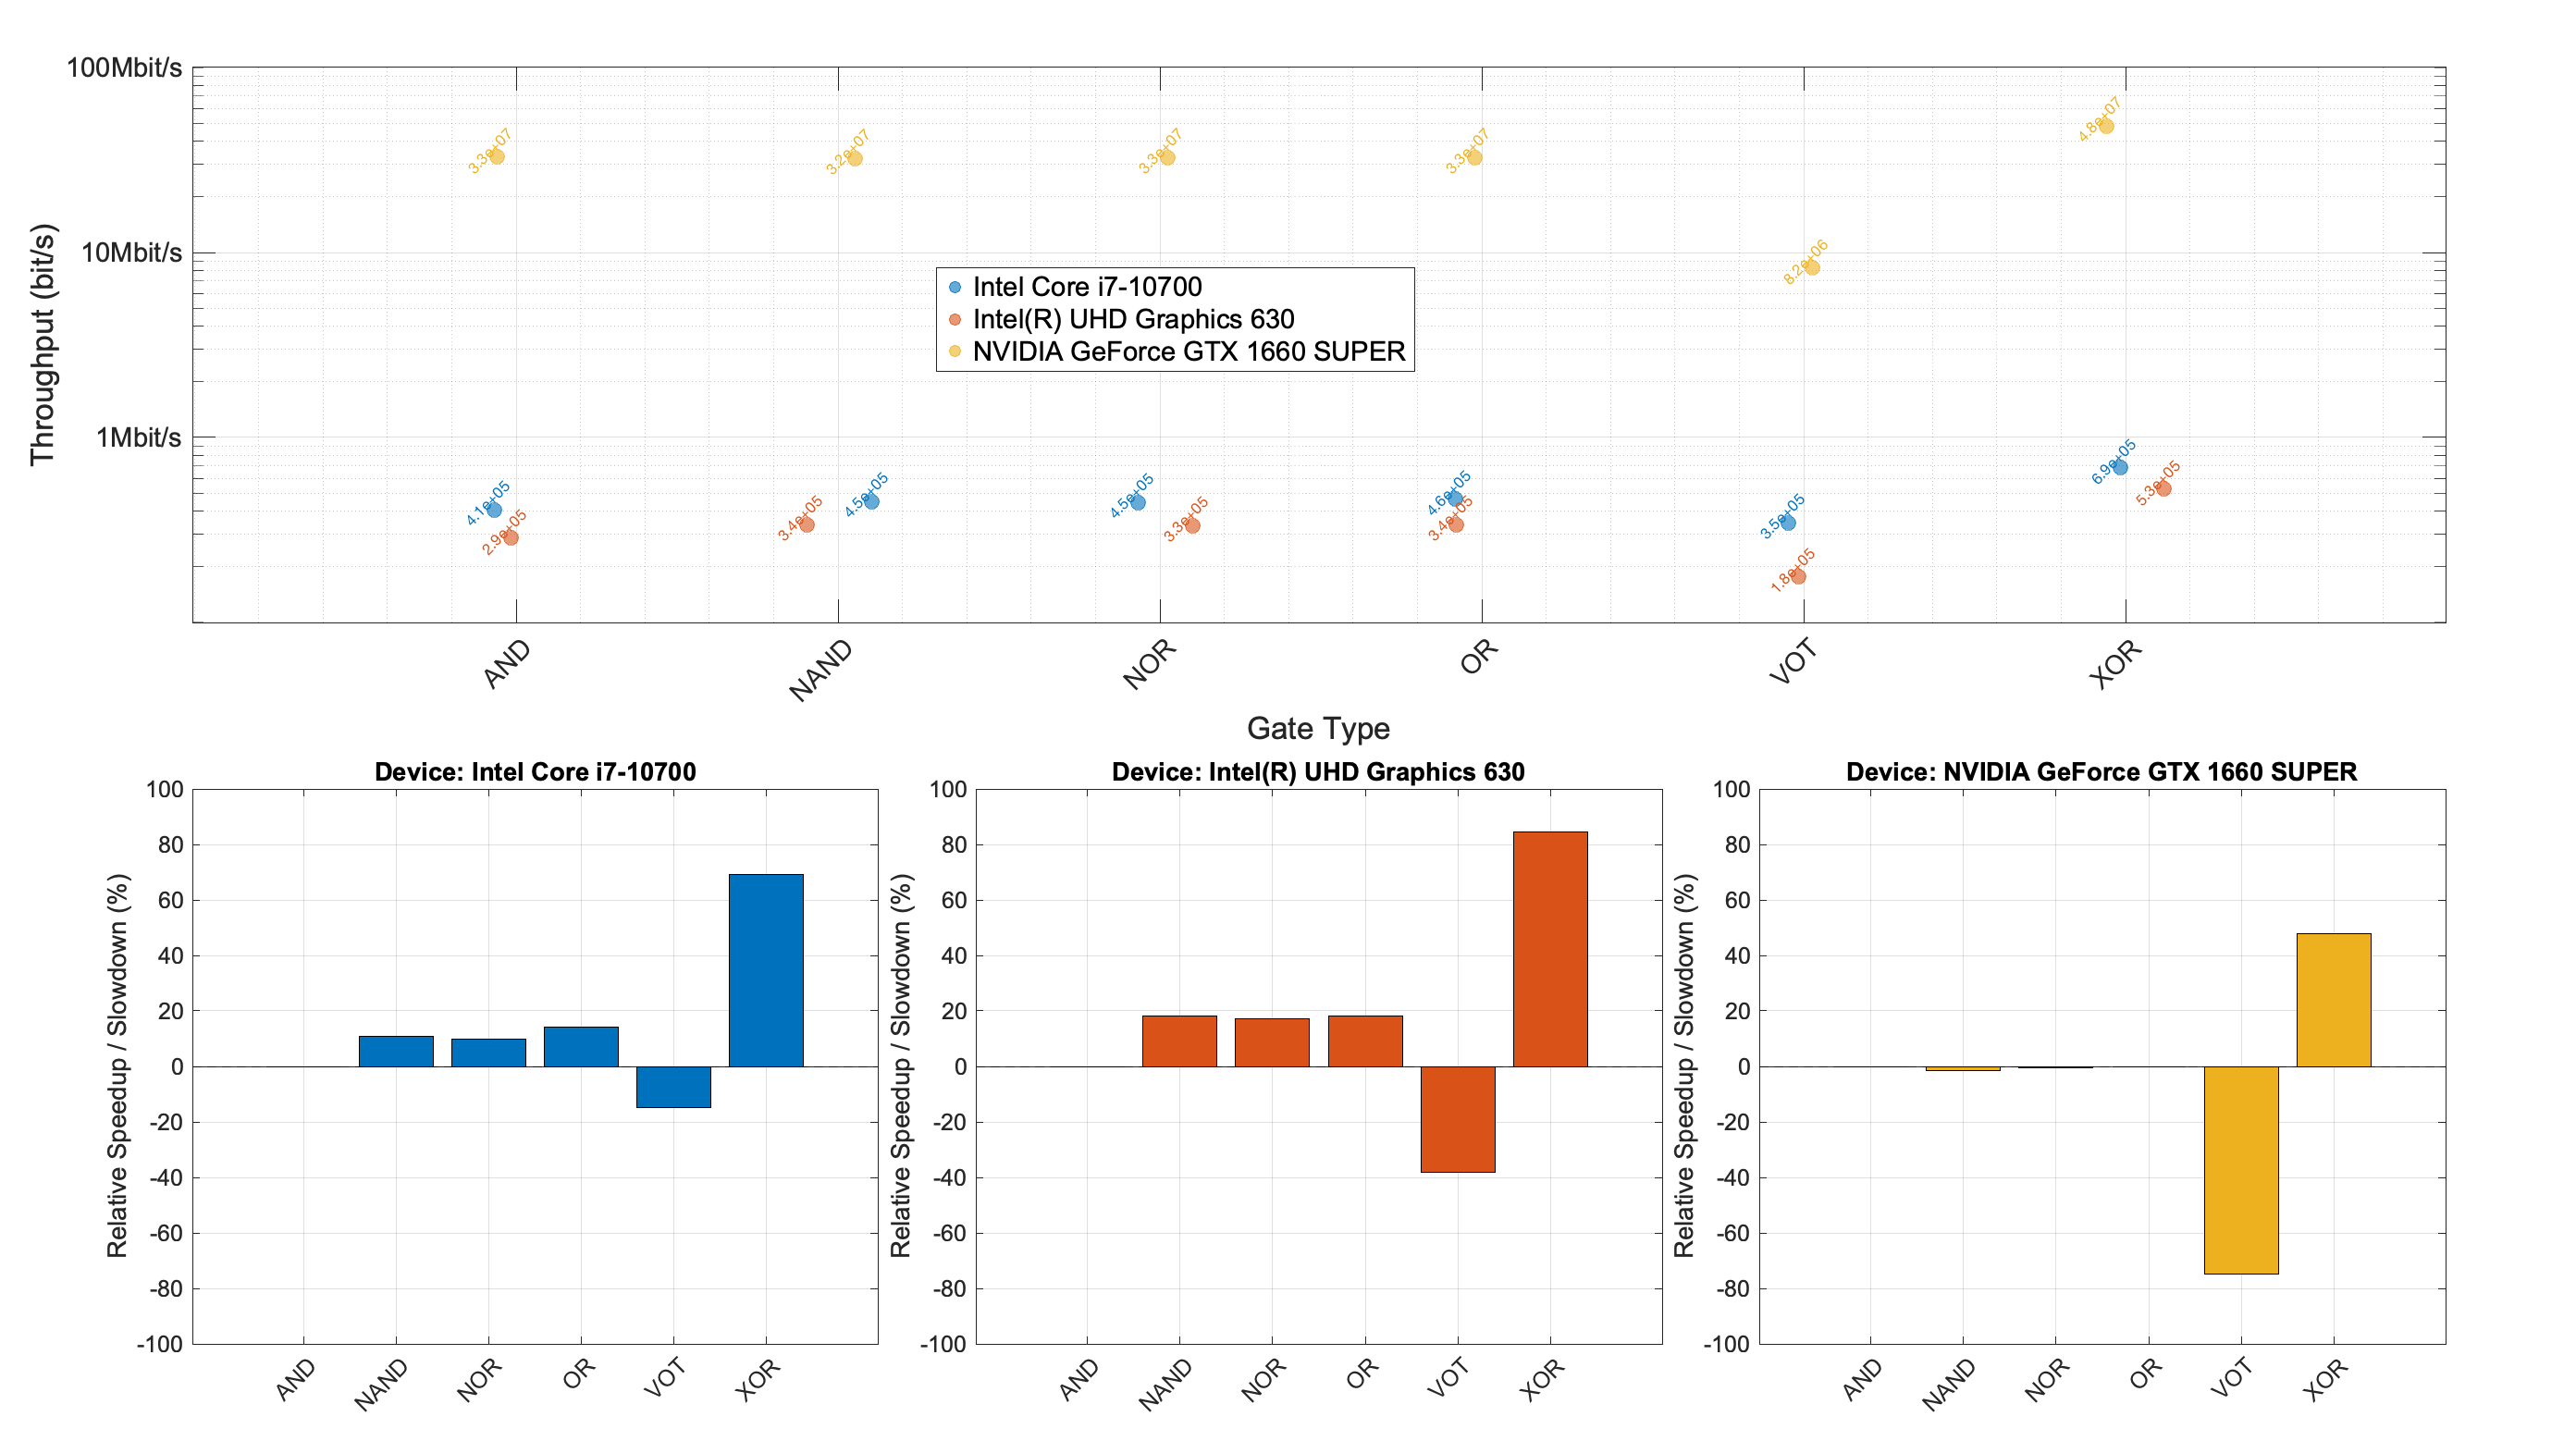
\includegraphics[height=0.8\textheight]{execution_model/slides_throughput_by_gate_type.eps}
    \caption{(Top) Throughput in bit/second on various backends for different gate types. (Bottom) \% Relative speedup/slowdown as compared to the AND gate.}
    \label{fig:gate_throughput}
\end{figure}

%% throughput graph
\begin{frame}{Eval Query Performance on Discrete GPUs}
  \begin{columns}
    \column{0.60\textwidth}
    {
      \begin{itemize}
          \item {Latency: 20-30 $ms$ per layer.}
          \item {Throughput: Graph depth and VRAM bound (see plot).}
          \item {Benchmarked on Nvidia GTX 1660 [6GB].}
          \item {Graph sizes: from $\approx 50$ to $\approx 2000$ nodes.}
          \item {Evals: from 16M to 1B per node per pass.}
      \end{itemize}
      \vspace{10pt}
      \textbf{Q: Are these enough samples to estimate the Expectation Query?}
    }
     \column{0.4\textwidth}
        \centering
        \includesvg[height=0.9\textheight]{1_concepts/mem_allocation_lines_zoom.svg}
  \end{columns}
\end{frame}





% ============================================================================
%  Research Objective 3 — Monte-Carlo Probability Estimation
%  Replaces prior preliminary version; integrates new pipeline & diagnostics
% ============================================================================
\section{Research Objective 3: Develop data-parallel Monte Carlo algorithms for probability estimation}

% ----------------------------------------------------------------------------
%  Title Frame
% ----------------------------------------------------------------------------
\begin{frame}
  \Large\centering\textbf{Research Objective 3}\\[6pt]
  \large Develop data-parallel Monte-Carlo methods for estimating probabilities on unified PDAGs
\end{frame}

% ----------------------------------------------------------------------------
%  Bridge: From Boolean Evaluation to Probabilistic Inference
% ----------------------------------------------------------------------------
\begin{frame}{Bridging Boolean Evaluation and Probabilistic Inference}
  \begin{itemize}
    \item Previous objective delivered \emph{bit-parallel gate kernels} that evaluate a PDAG layer in $\mathcal{O}(1)$ machine words.
    \item To quantify \alert{risk}, we must attach \emph{probability distributions} to the PDAG leaves and propagate forward.
    \item Strategy: embed a Monte-Carlo engine that
          \begin{enumerate}
            \item draws bit-packed Bernoulli samples for \textbf{all} basic events, and
            \item reuses the same gate kernels to evaluate each random draw.
          \end{enumerate}
    \item One kernel pipeline therefore suffices for \textbf{both} deterministic logic and stochastic sampling.
  \end{itemize}
\end{frame}

\subsection{Back to Working Example: One Initiating Event, Three Fault Trees, Six Basic Events, Five End States}
\begin{frame}
  \begin{columns}
    \column{0.66\textwidth}
      \includesvg[height=\textheight]{1_concepts/dag_pass_3.svg} % Replace with your image file
     \column{0.33\textwidth}
      \includesvg[width=\linewidth]{1_concepts/pra-model.svg} % Replace with your image file
  \end{columns}  
\end{frame}

% ----------------------------------------------------------------------------
%  End-to-End Sampling Pipeline
% ----------------------------------------------------------------------------
\begin{frame}{End-to-End Sampling Pipeline (one iteration)}
  \begin{columns}
    \column{0.6\textwidth}
      \includesvg[height=0.9\textheight]{1_concepts/dag_pass_3.svg} % Replace with your image file
     \column{0.4\textwidth}
  \tiny   
  \begin{enumerate}[<+->]
    \item \textbf{Basic-Event Kernel:} generate random draws.
    \item \textbf{Gate Kernels:} evaluate PDAG layers using hardware-native logic primitives.
    \item \textbf{Tally Kernel:} count number of ones, update counters, compute estimates.
  \end{enumerate}
  \end{columns}  
\end{frame}

% ----------------------------------------------------------------------------
%  Monte-Carlo Algorithm Recap (keeps most of prior text)
% ----------------------------------------------------------------------------
\subsection{MC Sampling Theory}

\begin{frame}{Monte-Carlo Sampling over PDAGs}
  \small
  \begin{enumerate}
    \item Draw $\mathbf{x}^{(i)}\sim\prod_{b\in\mathcal{B}}\text{Bernoulli}\bigl(p_b\bigr)$ in \textbf{bit-packed} form.
    \item Evaluate the Boolean function $F\colon\{0,1\}^{|\mathcal{B}|}\!\to\!\{0,1\}$ (root node) using the gate kernels.
    \item Record $Y^{(i)} \!=\! F\bigl(\mathbf{x}^{(i)}\bigr)$ \;(failure indicator).
  \end{enumerate}
  After $N$ iterations
  \[\widehat{P}_N = \frac1N\sum_{i=1}^N Y^{(i)},\qquad \operatorname{SE}(\widehat P_N)=\sqrt{\frac{\widehat P_N(1-\widehat P_N)}{N}}.\]
  Error shrinks as $\mathcal{O}\!\bigl(N^{-1/2}\bigr)$; variance-reduction extensions discussed shortly.
\end{frame}


% ----------------------------------------------------------------------------
%  Basic-Event Sampling Kernel
% ----------------------------------------------------------------------------
\begin{frame}{Basic-Event Sampling Kernel}
\begin{columns}
  \column{0.7\textwidth}
  \footnotesize
  \begin{itemize}
    \item Each basic event $b\in\mathcal{B}$ is modelled as an independent \textbf{Bernoulli} random variable $X_b\sim\operatorname{Bernoulli}(p_b)$.
    \item A single Monte--Carlo iteration packs $\omega = 8\,\mathrm{sizeof}(\texttt{bitpack\_t}) = 64$ independent trials into one machine word.
    \item For batch index $b$, bit--pack $p$, lane $\lambda$:
          $\displaystyle X_{b,p,\lambda}\sim\operatorname{Bernoulli}(p_b)$.
    \item The basic--event kernel uses the counter--based \textsc{Philox--4×32--10} PRNG; counters are derived from $(b,p,\lambda,t)$, guaranteeing reproducibility and inter--thread independence.
    \item After one iteration ($N = B P \omega$ trials) the sufficient statistics per basic event are
          $\displaystyle s_b = \sum_{p,\lambda} X_{b,p,\lambda}$,\;
          $\widehat p_b = s_b/N$,\;
          $\operatorname{SE}(\widehat p_b)=\sqrt{\widehat p_b(1-\widehat p_b)/N}$.
  \end{itemize}
       \column{0.3\textwidth}
       \includesvg[width=\textwidth]{2_framework/research_objective_3_mc_sampling/sample_event_A.svg}\par
  \end{columns}
\end{frame}


%% needs a frame on tallies, with estimator statistics, convergence properties
% ----------------------------------------------------------------------------
%  Tally Kernel & Estimator Convergence
% ----------------------------------------------------------------------------
\begin{frame}{Tally Kernel}
  \footnotesize
  \begin{itemize}
    \item For a designated node $v$ (e.g. system top event) define $Y_{p,\lambda}^{(t)} = F_v\bigl(\mathbf{X}_{\cdot,p,\lambda}^{(t)}\bigr)\in\{0,1\}$.
    \item \textbf{Tally kernel} executes a single SIMD \texttt{popcount} per bit-pack to obtain the per-iteration count
      $\displaystyle s_v^{(t)} = \sum_{p,\lambda} Y_{p,\lambda}^{(t)}$.
    \item Cumulative statistics after $T$ iterations ($N_T = T N$ trials):
      \[ S_v = \sum_{t=1}^{T} s_v^{(t)},\qquad \widehat P_v = \frac{S_v}{N_T}. \]
    \item Unbiased variance estimator
      \[ \widehat{\sigma}^2_v = \frac{\widehat P_v\bigl(1-\widehat P_v\bigr)}{N_T}. \]
    \item \textbf{Central Limit Theorem.}  As $T\to\infty$
      \[ \frac{\widehat P_v - P_v}{\widehat \sigma_v}\;\xrightarrow{\,\mathcal{D}\,}\;\mathcal N(0,1). \]
  \end{itemize}
\end{frame}

%% run with runaway iterations.
%% show a run with too many iterations, and make the case for developing a robust convergence criteria.
% ----------------------------------------------------------------------------
%  The Cost of Runaway Iterations (Motivation)
% ----------------------------------------------------------------------------
\begin{frame}{When "More Samples" is Wasteful}
  \begin{columns}
    \column{0.35\textwidth}
      \footnotesize
      \begin{itemize}
        \item Fixed iteration budgets ($N$ large and hard-wired) risk \emph{massive}\, oversampling when $P_v$ is moderate (\(\approx10^{-4}\)–\(10^{-1}\)).
      \end{itemize}
    \column{0.65\textwidth}
      \centering
      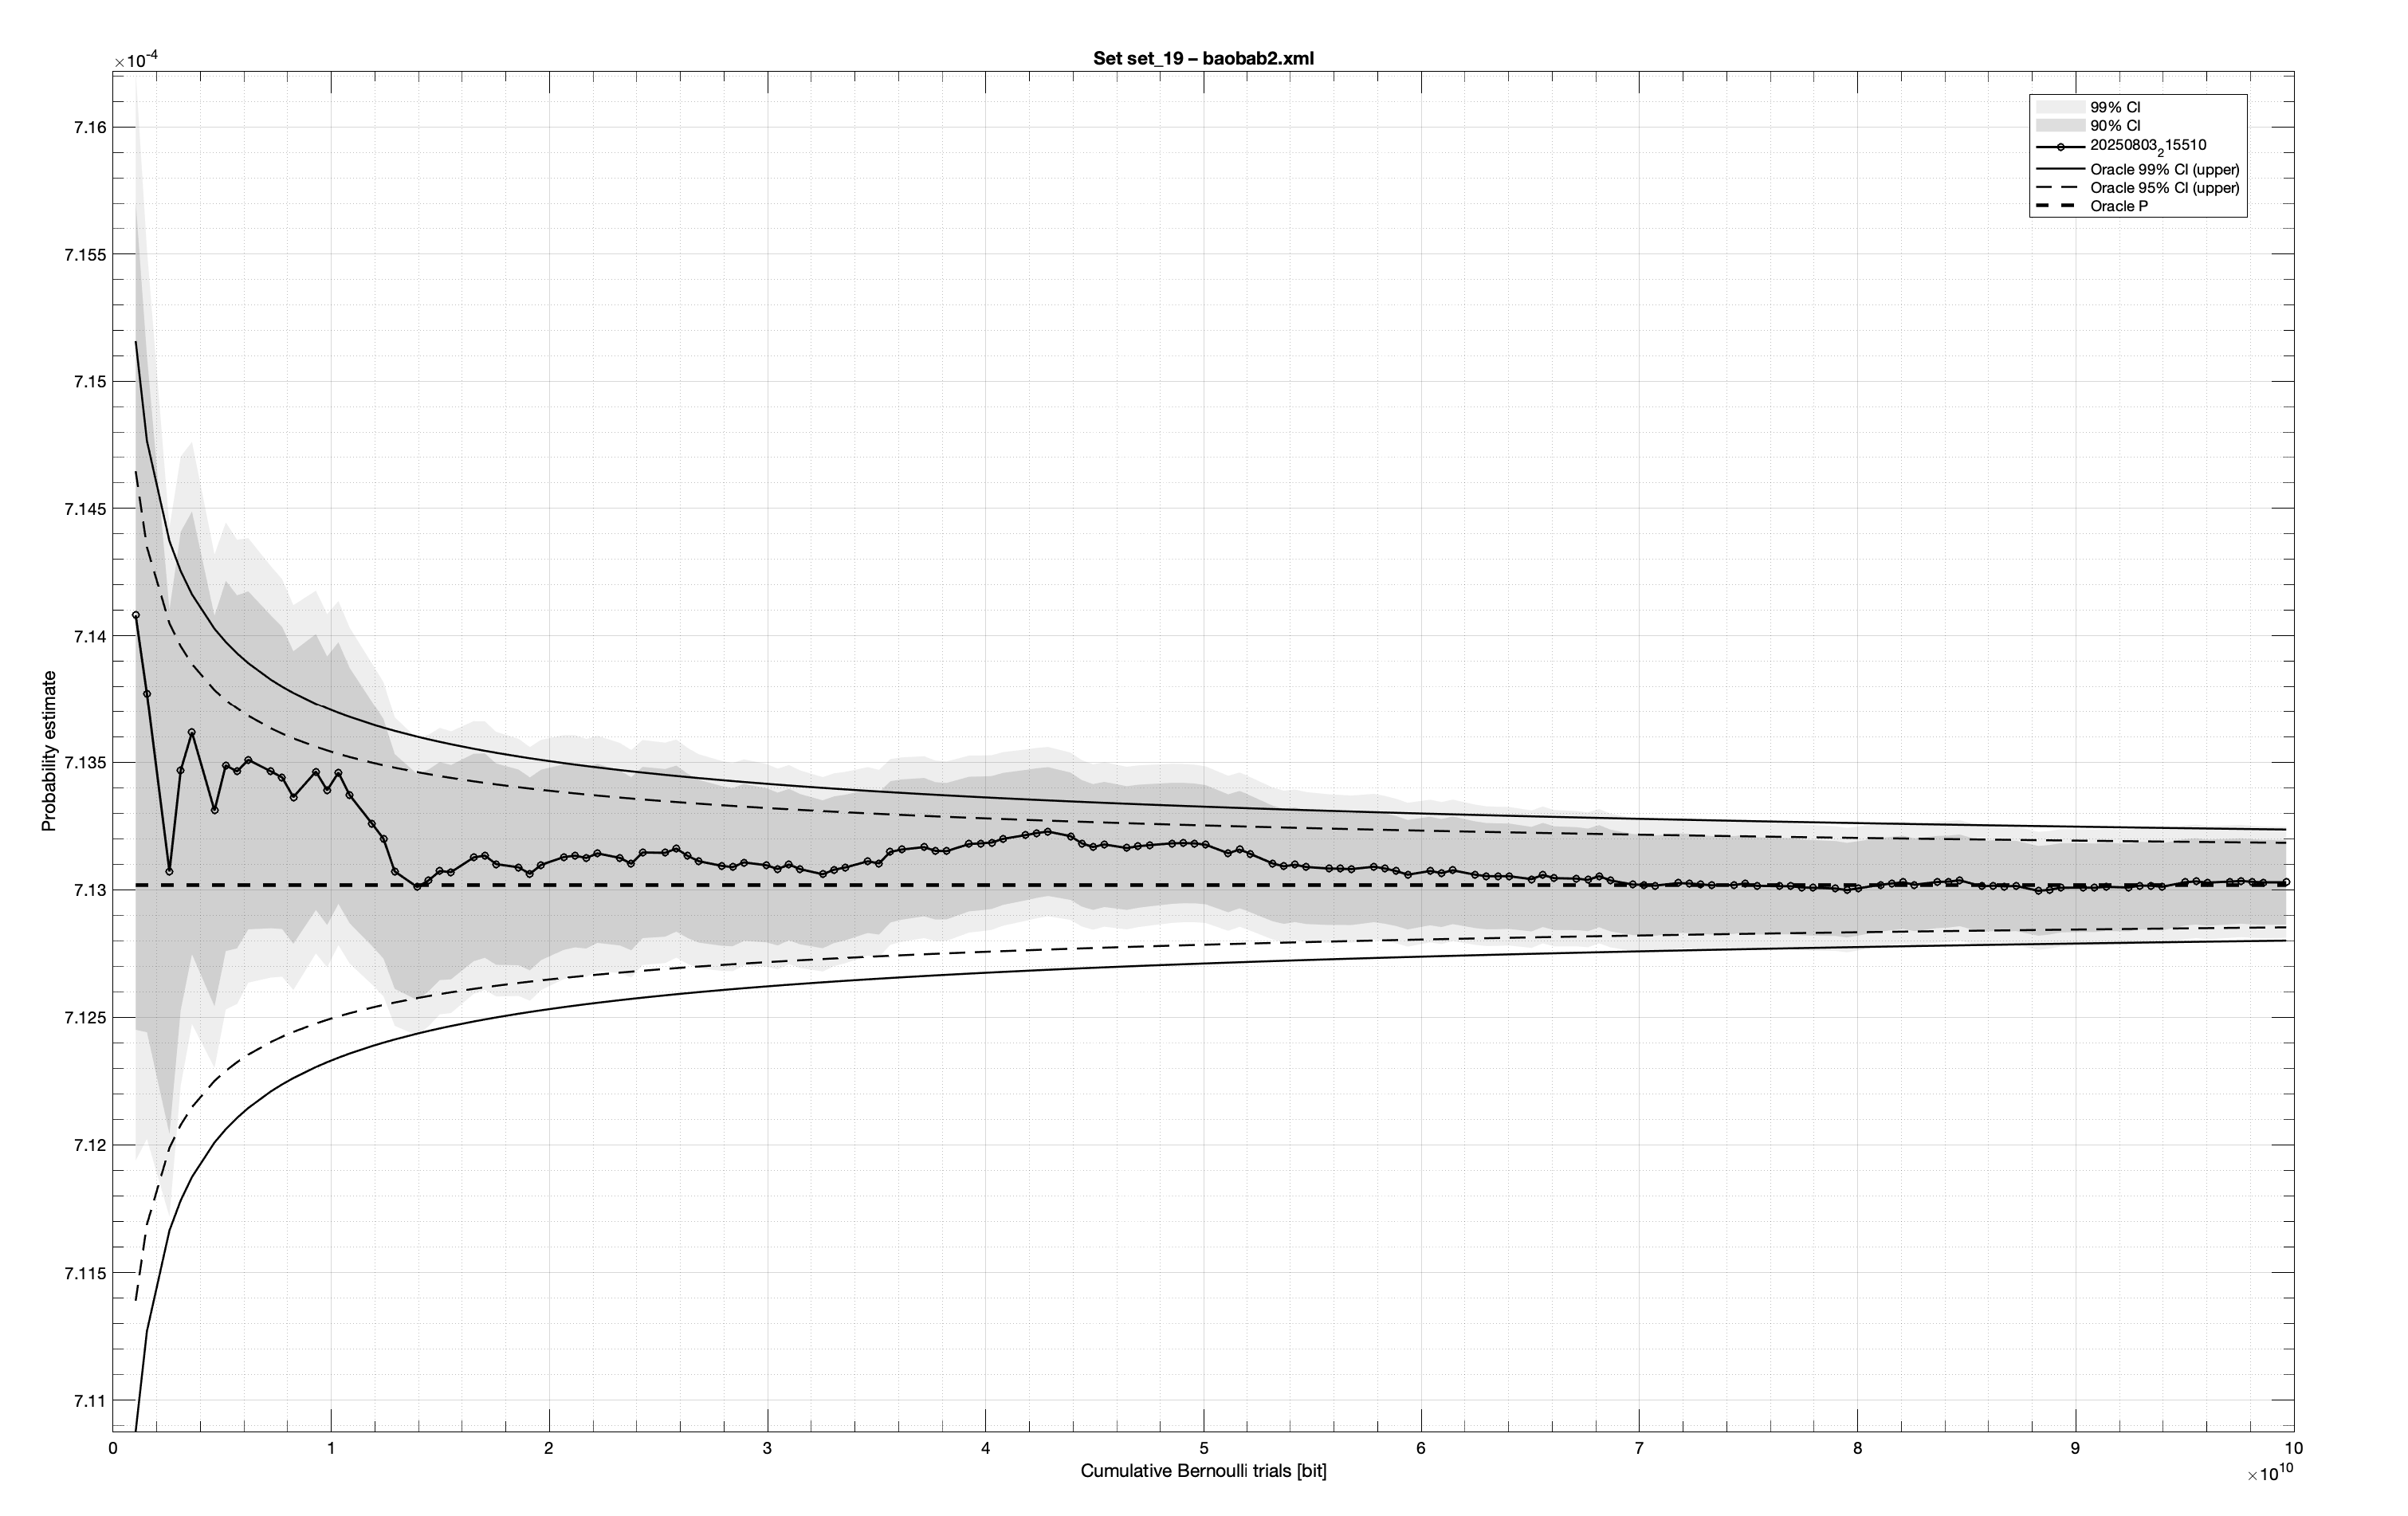
\includegraphics[width=0.95\linewidth]{2_framework/research_objective_3_mc_sampling/conv_fig_02.eps} % create trace: half-width vs iterations
      \vspace{-6pt}
  \end{columns}
\end{frame}


\section{Research Objective 4: Convergence Guarantees}
\begin{frame}
    \Large{\centerline{\textbf{Research Objective 4}}}
    \vspace{6pt}
    \large{\centerline{\textbf{Develop Robust Convergence Criteria}}}
\end{frame}
\subsection{Interpretation of Probability}
% ------------------------------------
%  Criterion 1 – Frequentist Half-Width
% ------------------------------------
\begin{frame}{Criterion 1: Frequentist Half-Width (Wald)}
  \footnotesize
  Let $\{Y^{(i)}\}_{i=1}^N$ be i.i.d. Bernoulli trials with $P=\Pr[Y=1]$.  The estimator $\widehat P_N=\tfrac1N\sum_i Y^{(i)}$ obeys the CLT:
  \[\sqrt{N}\,\bigl(\widehat P_N-P\bigr) \;\xrightarrow{d}\; \mathcal N\bigl(0, P(1-P)\bigr).\]
  A $(1-\alpha)$ two–sided \textbf{Wald} interval is therefore
  \[ \widehat P_N \;\pm\; z_{1-\alpha/2}\, \sqrt{\tfrac{\widehat P_N(1-\widehat P_N)}{N}}. \]
  \begin{alertblock}{Stopping rule}
   \textbf{Half-width:} $h_N^{\text{lin}}(z)=z\sqrt{\widehat P_N(1-\widehat P_N)/N}.$ Declare convergence when $h_N^{\text{lin}}/\widehat P_N\le \varepsilon_{\text{rel}}$.
  \end{alertblock}
  \begin{block}{Intuition}
    Shrinks a \emph{relative} confidence band around the estimate; fast for moderate $P$, slow for rare events where $\widehat P_N\ll10^{-4}$.
  \end{block}
\end{frame}

% ------------------------------------
%  Criterion 2 – Bayesian Credible Interval
% ------------------------------------
\begin{frame}{Criterion 2: Bayesian Credible Interval (Jeffreys prior)}
  \footnotesize
  Prior $p\sim\text{Beta}\bigl(\tfrac12,\tfrac12\bigr)$ is invariant under re-parameterization.  After $s$ successes and $f$ failures the posterior is
  \[ p\mid\text{data}\;\sim\; \text{Beta}\bigl(s+\tfrac12,\,f+\tfrac12\bigr). \]
  The central $(1-\alpha)$ credible interval $[q_t,q_{1-t}]$ with $t=\alpha/2$ has
  \begin{alertblock}{Stopping rule}
  \textbf{half-width} $h_N^{\text{Bayes}}=(q_{1-t}-q_t)/2$. Convergence when $h_N^{\text{Bayes}}/\widehat P_N\le \varepsilon_{\text{rel}}^{\text{Bayes}}$.
  \end{alertblock}
  \begin{block}{Intuition}
  Integrates parameter uncertainty; maintains correct coverage even when $\widehat P_N$ is based on only a handful of observed failures (rare-event tails).
  \end{block}
\end{frame}

% ------------------------------------
%  Criterion 3 – Information Gain
% ------------------------------------
\begin{frame}{Criterion 3: Information-Theoretic Gain}
  \small
  Posterior entropy of $\text{Beta}(\alpha,\beta)$ is
  \[ H(\alpha,\beta)=\ln B(\alpha,\beta)- (\alpha-1)\psi(\alpha)- (\beta-1)\psi(\beta)+ (\alpha+\beta-2)\psi(\alpha+\beta). \]
  After a batch $(\Delta s,\Delta f)$ the \textbf{information gain} is
  \[ I_{\text{batch}} = H(\alpha,\beta) - H(\alpha+\Delta s,\,\beta+\Delta f). \]
  \begin{alertblock}{Stopping rule}
   Stop when $I_{\text{batch}}<I_{\min}$ bits (default $10^{-4}$).
  \end{alertblock}
  \begin{block}{Intuition}
 Scale-free; halts when each new batch conveys negligible Shannon information, preventing oversampling when $P$ is either very small or very large.
  \end{block}
\end{frame}

% ----------------------------------------------------------------------------
%  Composite Convergence Diagnostics
% ----------------------------------------------------------------------------
\begin{frame}{Composite Convergence Diagnostics}
  \begin{columns}
    \column{0.55\textwidth}
      \begin{itemize}
        \item \textbf{Frequentist half-width} $h_v(z)$ on linear and log scale.
        \item \textbf{Bayesian credible interval} with Jeffreys prior.
        \item \textbf{Information gain} $I_{\text{batch}}<10^{-4}$ bits.
        \item Run stops when \emph{all} criteria satisfied for every monitored node.
            \item \textbf{Composite stopping rule.}  Convergence declared when
      \[
        \frac{z_{1-\alpha/2}\,\widehat \sigma_v}{\widehat P_v} \le \varepsilon_{\text{rel}},\quad
        h^{\log}_v(z) \le \varepsilon^{\log},\quad
        I_{\text{batch}} < 10^{-4}\;\text{bits}.
      \]
      \end{itemize}
    \column{0.45\textwidth}
      \includegraphics[width=\linewidth]{2_framework/research_objective_3_mc_sampling/ci_trace.pdf} % create a small diagnostic trace figure
  \end{columns}
\end{frame}




\section{Research Objective 5: Case Studies and Benchmarks}
\begin{frame}
    \Large{\centerline{\textbf{Research Objective 5}}}
    \vspace{6pt}
    \large{\centerline{\textbf{Case Studies and Benchmarks}}}
\end{frame}

\subsection{Aralia Fault Tree Data Set}
\begin{frame}[t]
\frametitle{Overview: Aralia Dataset}
\begin{itemize}
  \item \textbf{Dataset Composition:} The Aralia collection consists of 43 distinct fault trees, each with varying numbers of basic events (BEs), gate types (AND, OR, K/N, XOR), and minimal cut-set counts.  
  \item \textbf{Diverse Problem Sizes:} Small trees (e.g.\ 25--32 BEs) through large models with over 1{,}500 BEs.  
  \item \textbf{Wide Probability Range:} Top-event probabilities spanning from rare events near \(10^{-13}\) to fairly likely failures with probability above 0.7.  
  \item \textbf{Model Variability:} Some trees are primarily AND/OR, others incorporate more advanced gates (K/N, XOR, NOT), providing thorough coverage of typical (and atypical) fault tree logic structures.
\end{itemize}
\end{frame}

\begin{frame}[allowframebreaks]
    \input{4_casestudy/3_table_aralia_ft_dataset}
\end{frame}

\subsection{Benchmarking Procedure}
\begin{frame}[t]
\frametitle{Benchmarking Setup: Hardware and Environment}
\begin{itemize}
  \item \textbf{Target Hardware:}
    \begin{itemize}
      \item GPU: NVIDIA\textsuperscript{\textregistered} GeForce GTX 1660 SUPER (6\,GB GDDR6, 1{,}408 CUDA cores).
      \item CPU: Intel\textsuperscript{\textregistered} Core\textsuperscript{TM} i7-10700 (2.90\,GHz, turbo-boost, hyperthreading).
    \end{itemize}
  \item \textbf{Software Stack:}
    \begin{itemize}
      \item SYCL-based (AdaptiveCpp/HipSYCL), with LLVM-IR JIT for kernel compilation.
      \item Compiler optimization at \texttt{-O3} for efficient code generation.
      \item Repeated runs (5+) to mitigate transient variations.
    \end{itemize}
  \item \textbf{Measured Time:} Includes entire wall-clock duration, from host-device transfers and JIT compilation to final result collection.
\end{itemize}
\end{frame}

\subsection{Accuracy Benchmarks}
\begin{frame}
    \begin{figure}[h]
    \centering
    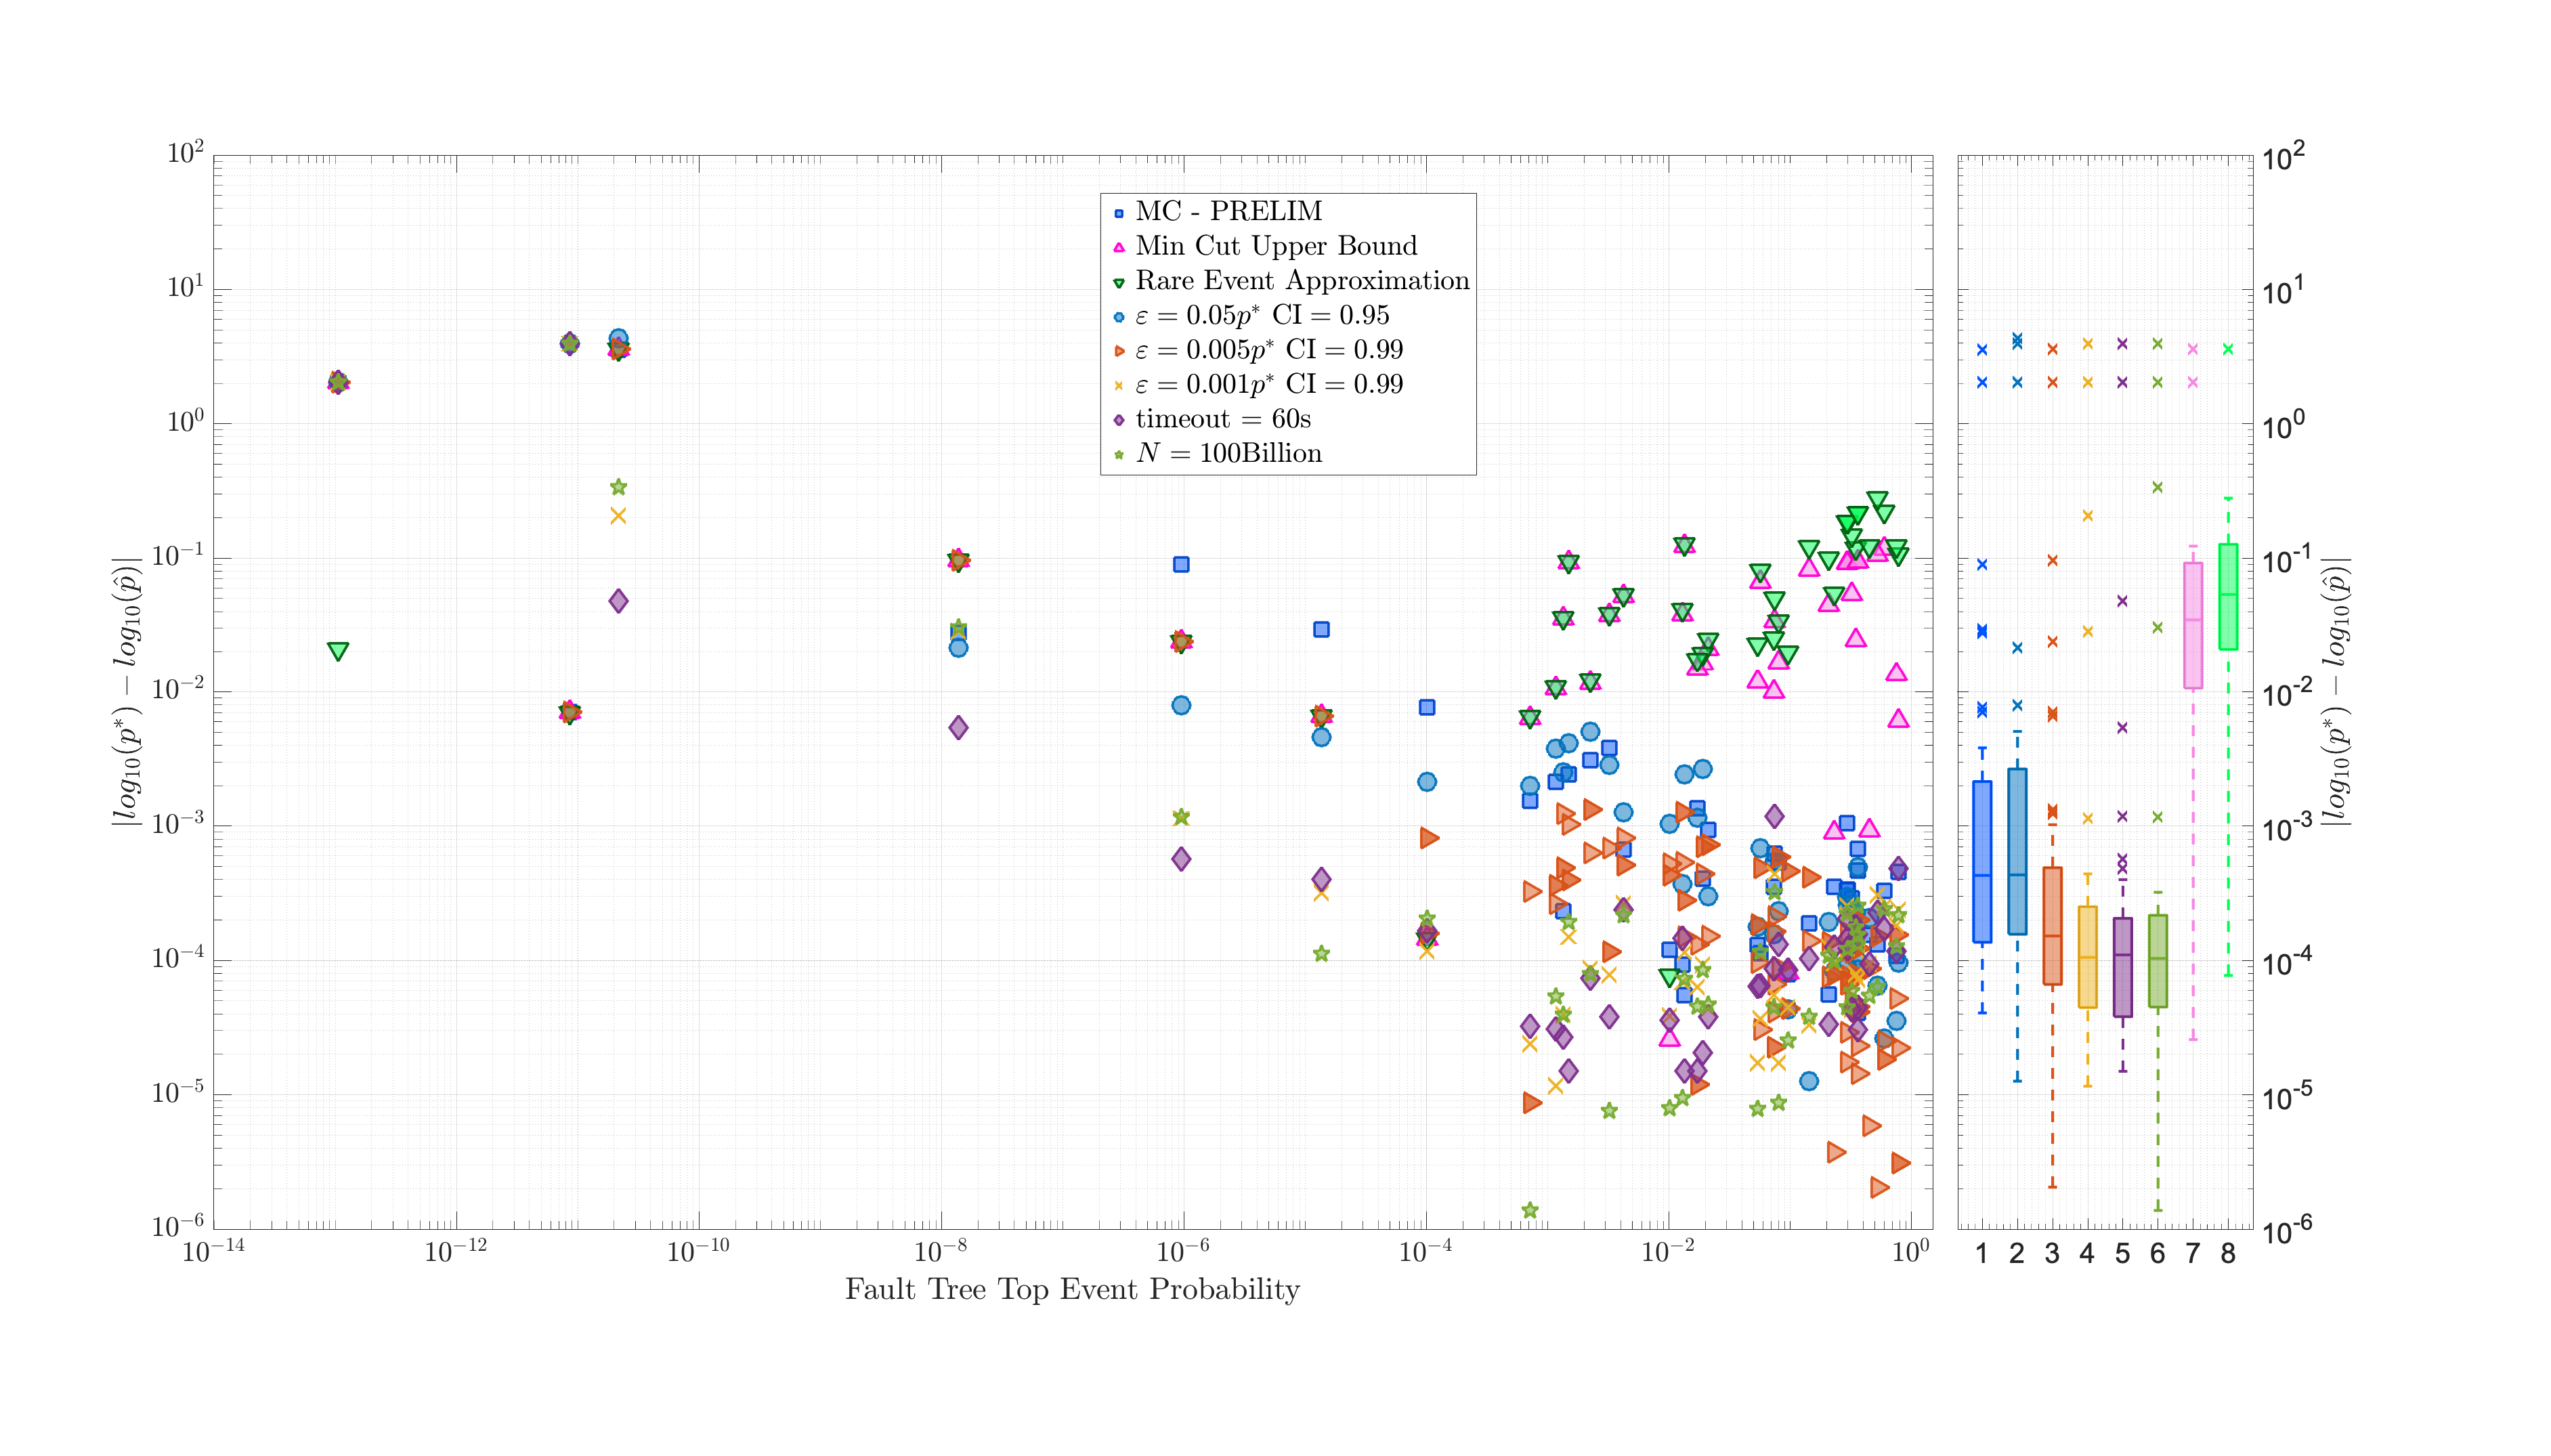
\includegraphics[height=1.1\textheight]{4_casestudy/abs_err.eps}
    \label{fig:mae_vs_logp}
\end{figure}
\end{frame}

\subsection{Accuracy vs. Time to Convergence}
\begin{frame}
\begin{figure}[p]
    \centering
    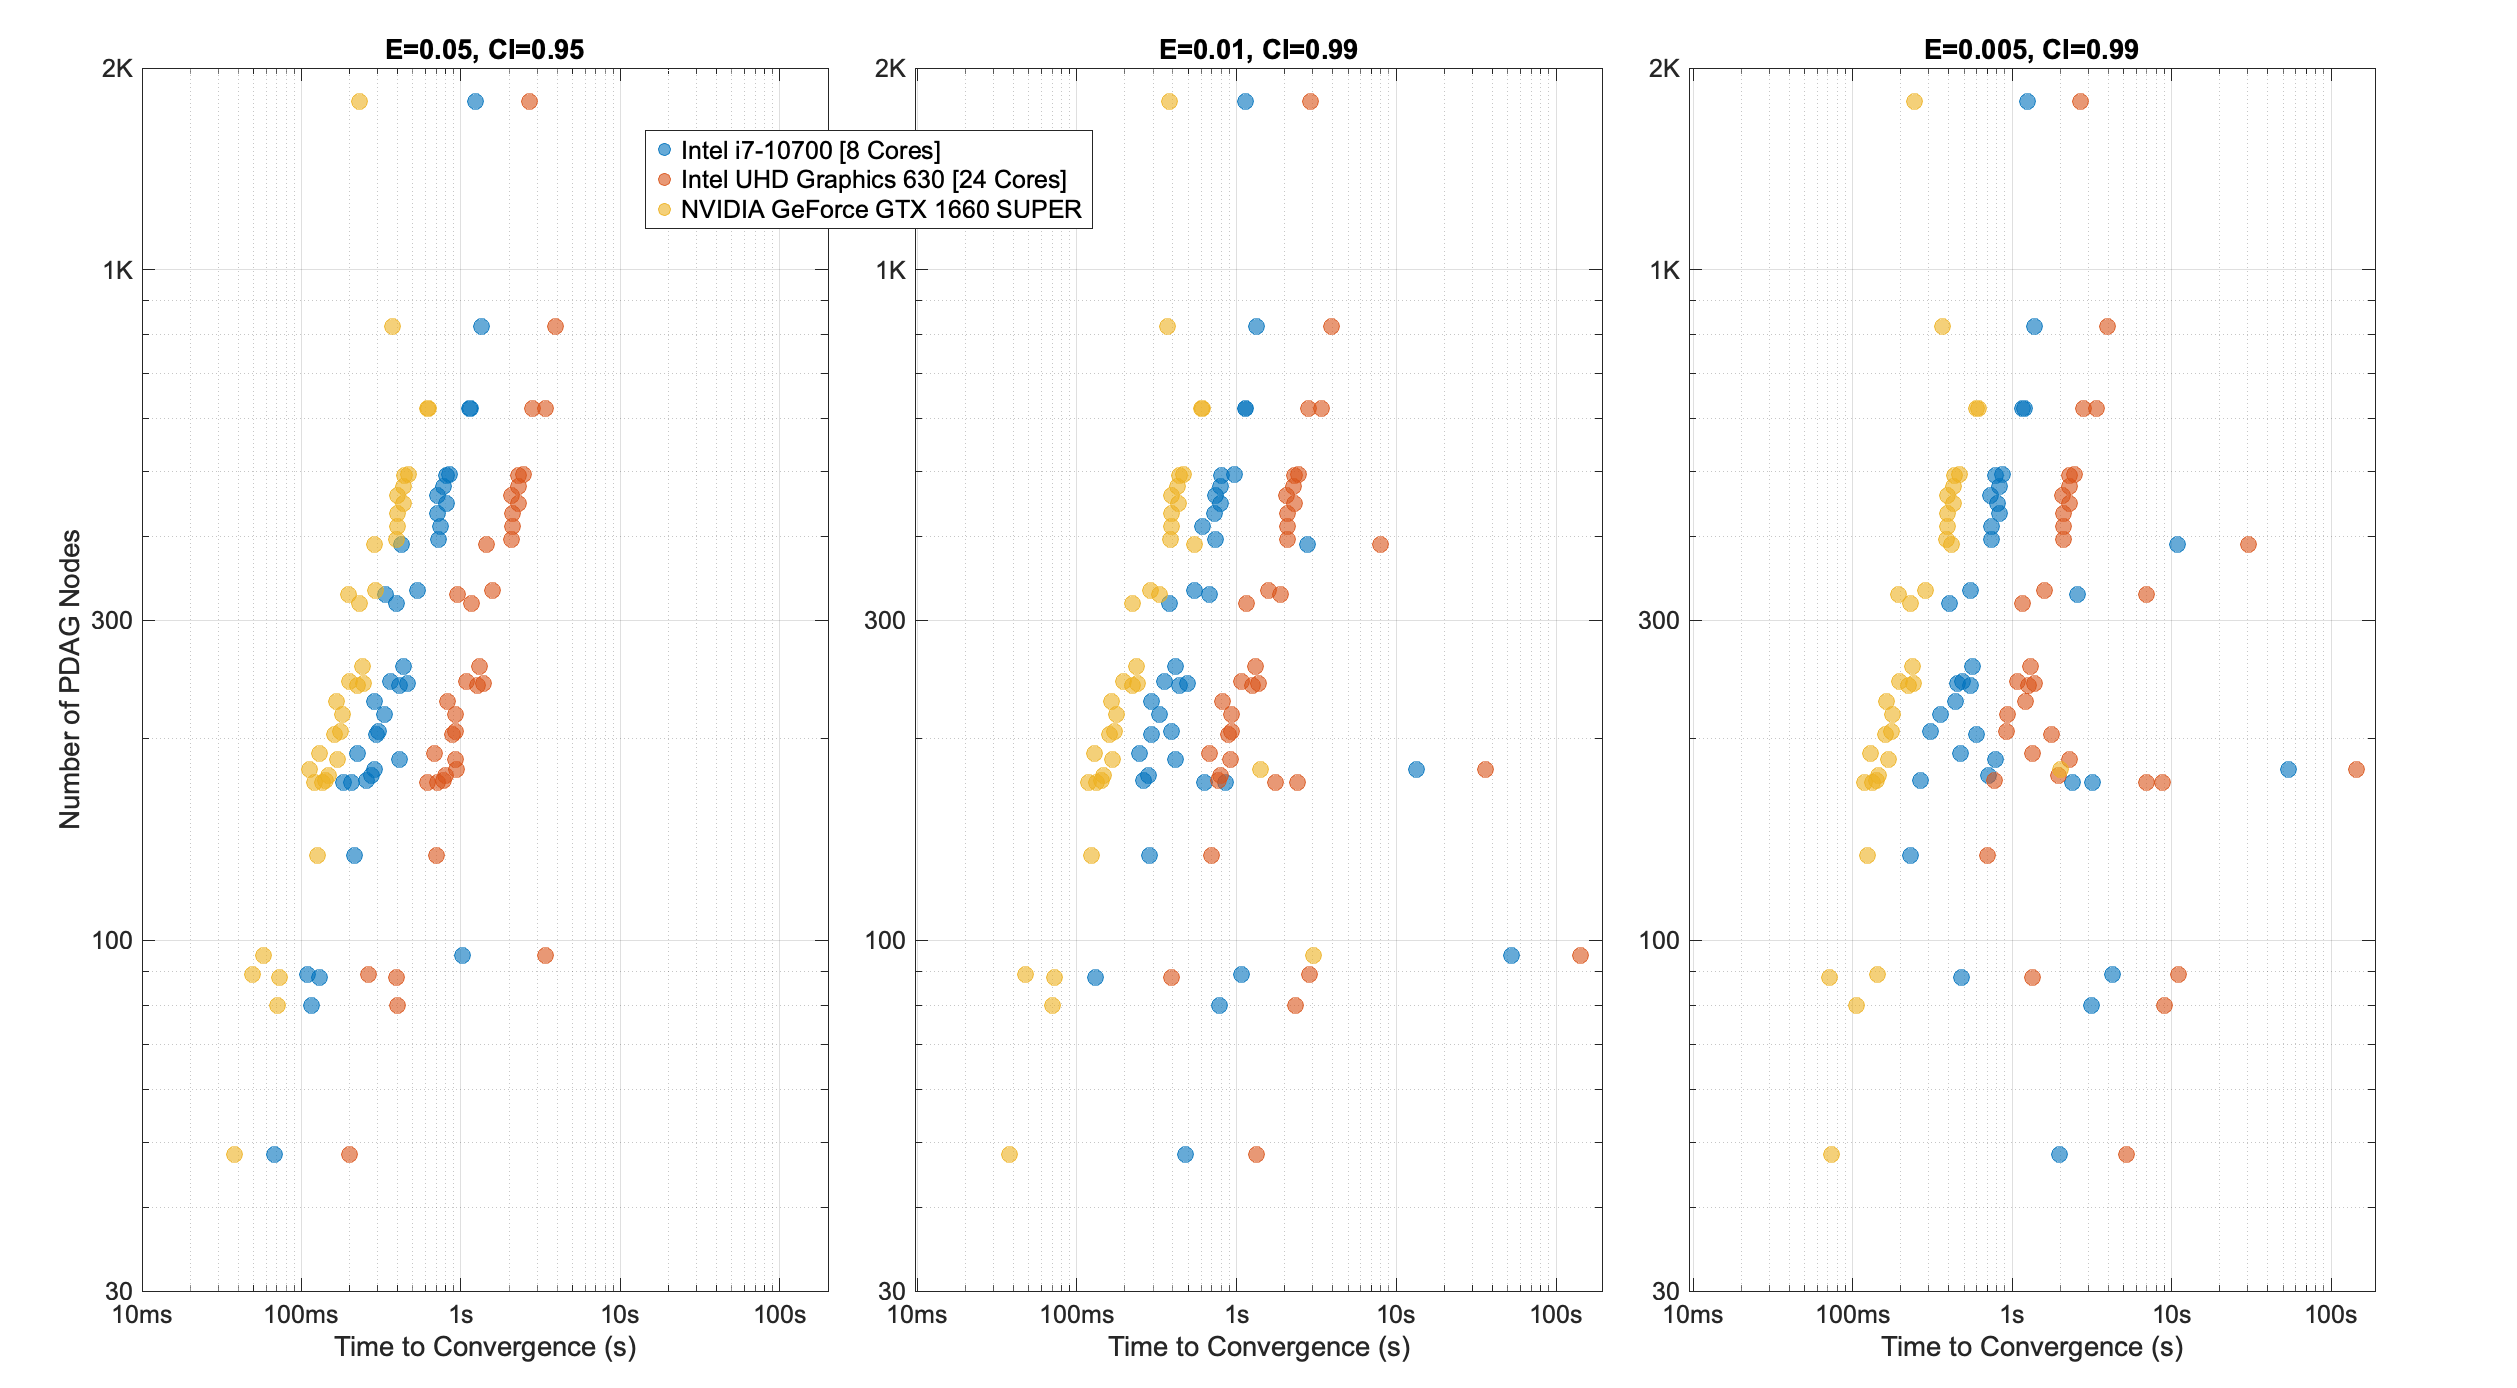
\includegraphics[height=1\textheight]{4_casestudy/throughput/slides_nodes_vs_convergence.eps}
    \caption{Time to convergence for different accuracy targets.}
    \label{fig:nodes_vs_convergence}
\end{figure}
\end{frame}

\subsection{Convergence Runs}
\begin{frame}
\begin{figure}[p]
    \centering
    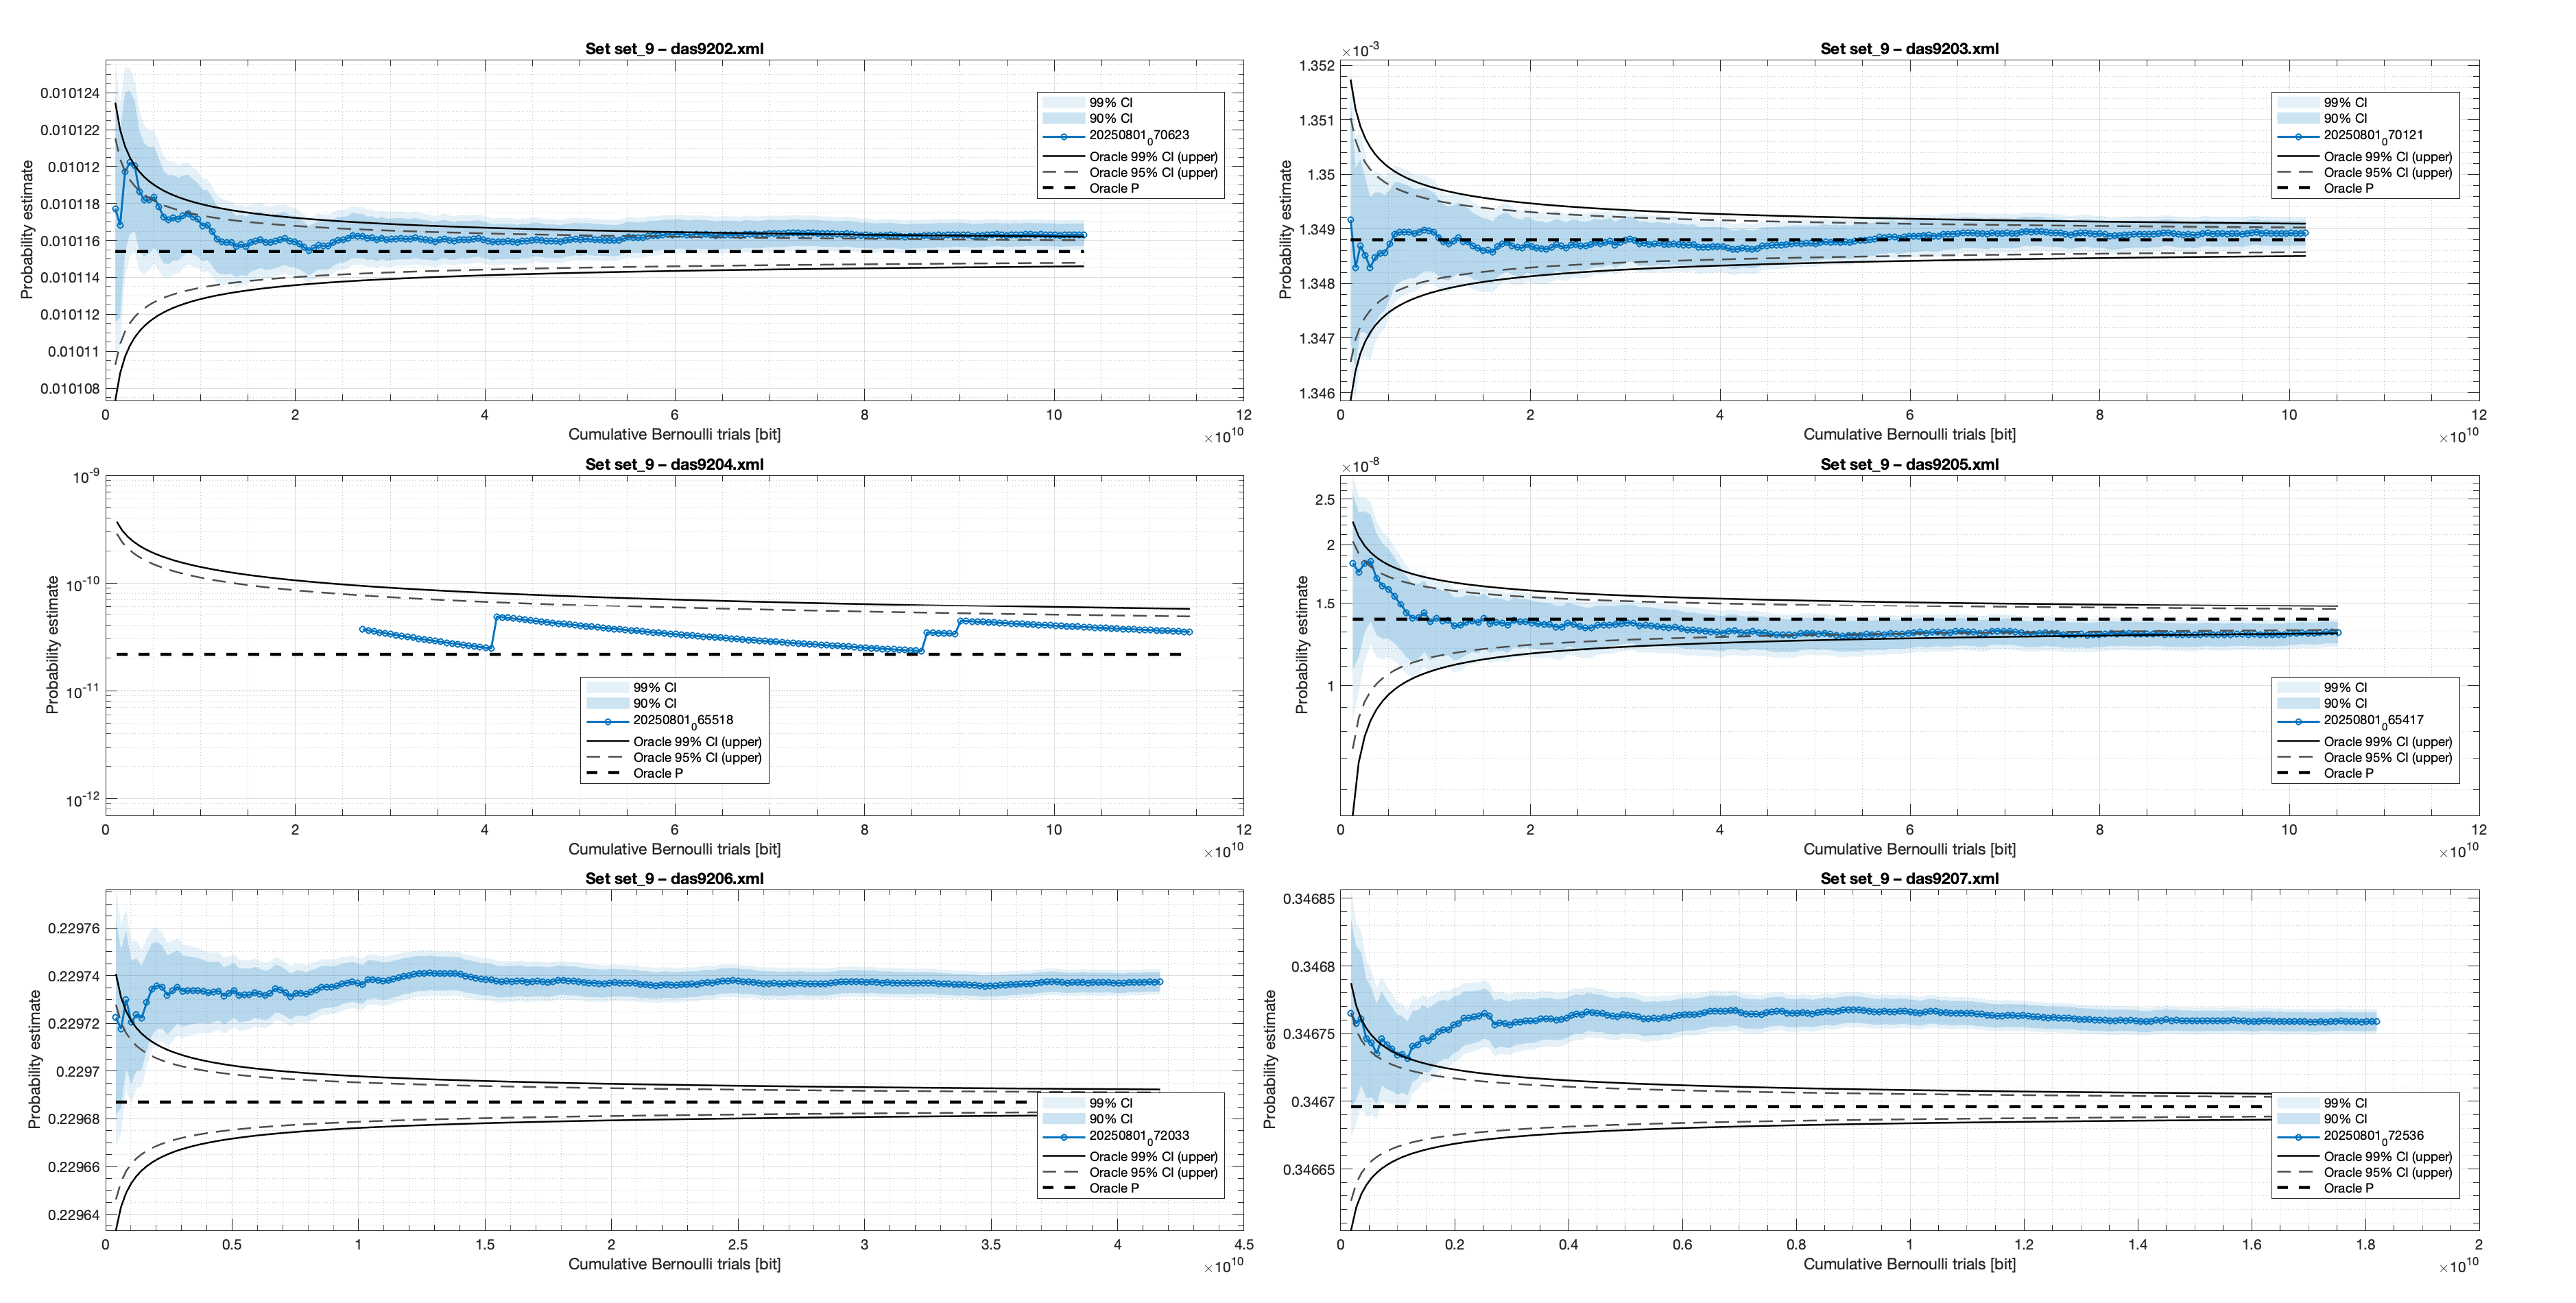
\includegraphics[height=1\textheight]{4_casestudy/conv_raw.eps}
    \label{fig:convergence_run_01}
\end{figure}
\end{frame}

\subsection{Convergence Runs, Comparison with MCUB, REA}
\begin{frame}
\begin{figure}[p]
    \centering
    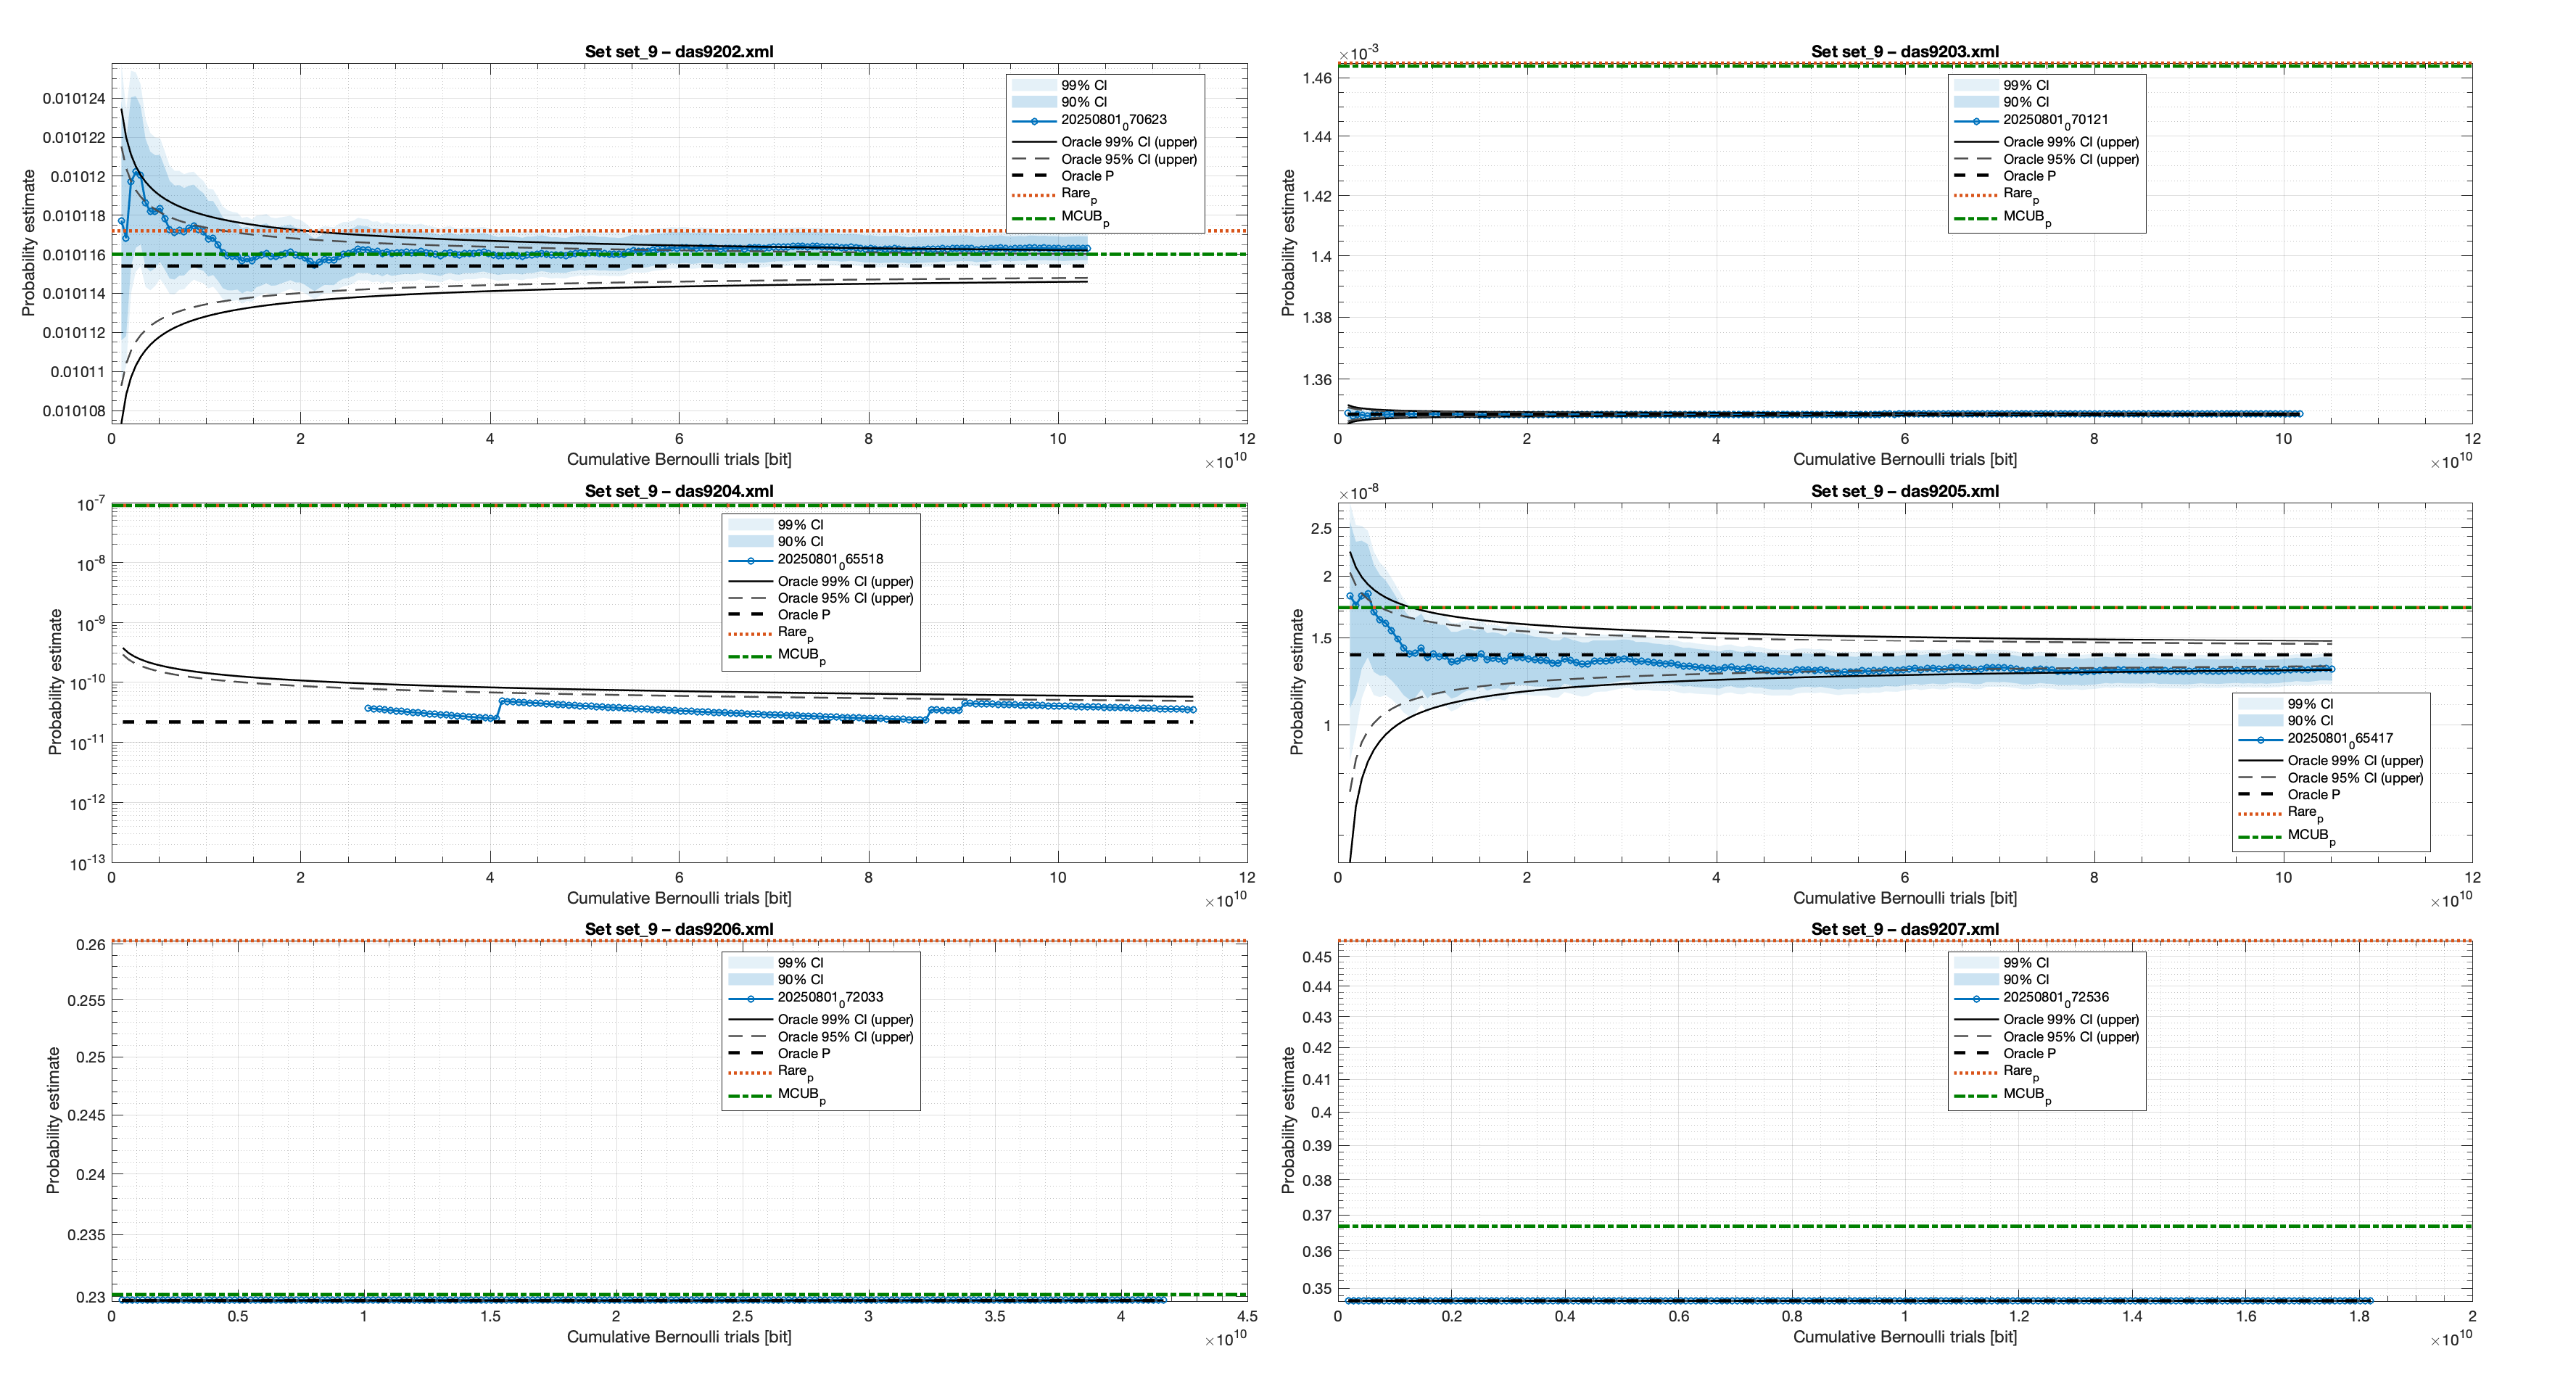
\includegraphics[height=1\textheight]{4_casestudy/conv_figeps.eps}
    \label{fig:convergence_run_01}
\end{figure}
\end{frame}

\subsection{Convergence Run -- Rare Event, Comparison with MCUB}
\begin{frame}
\begin{figure}[p]
    \centering
    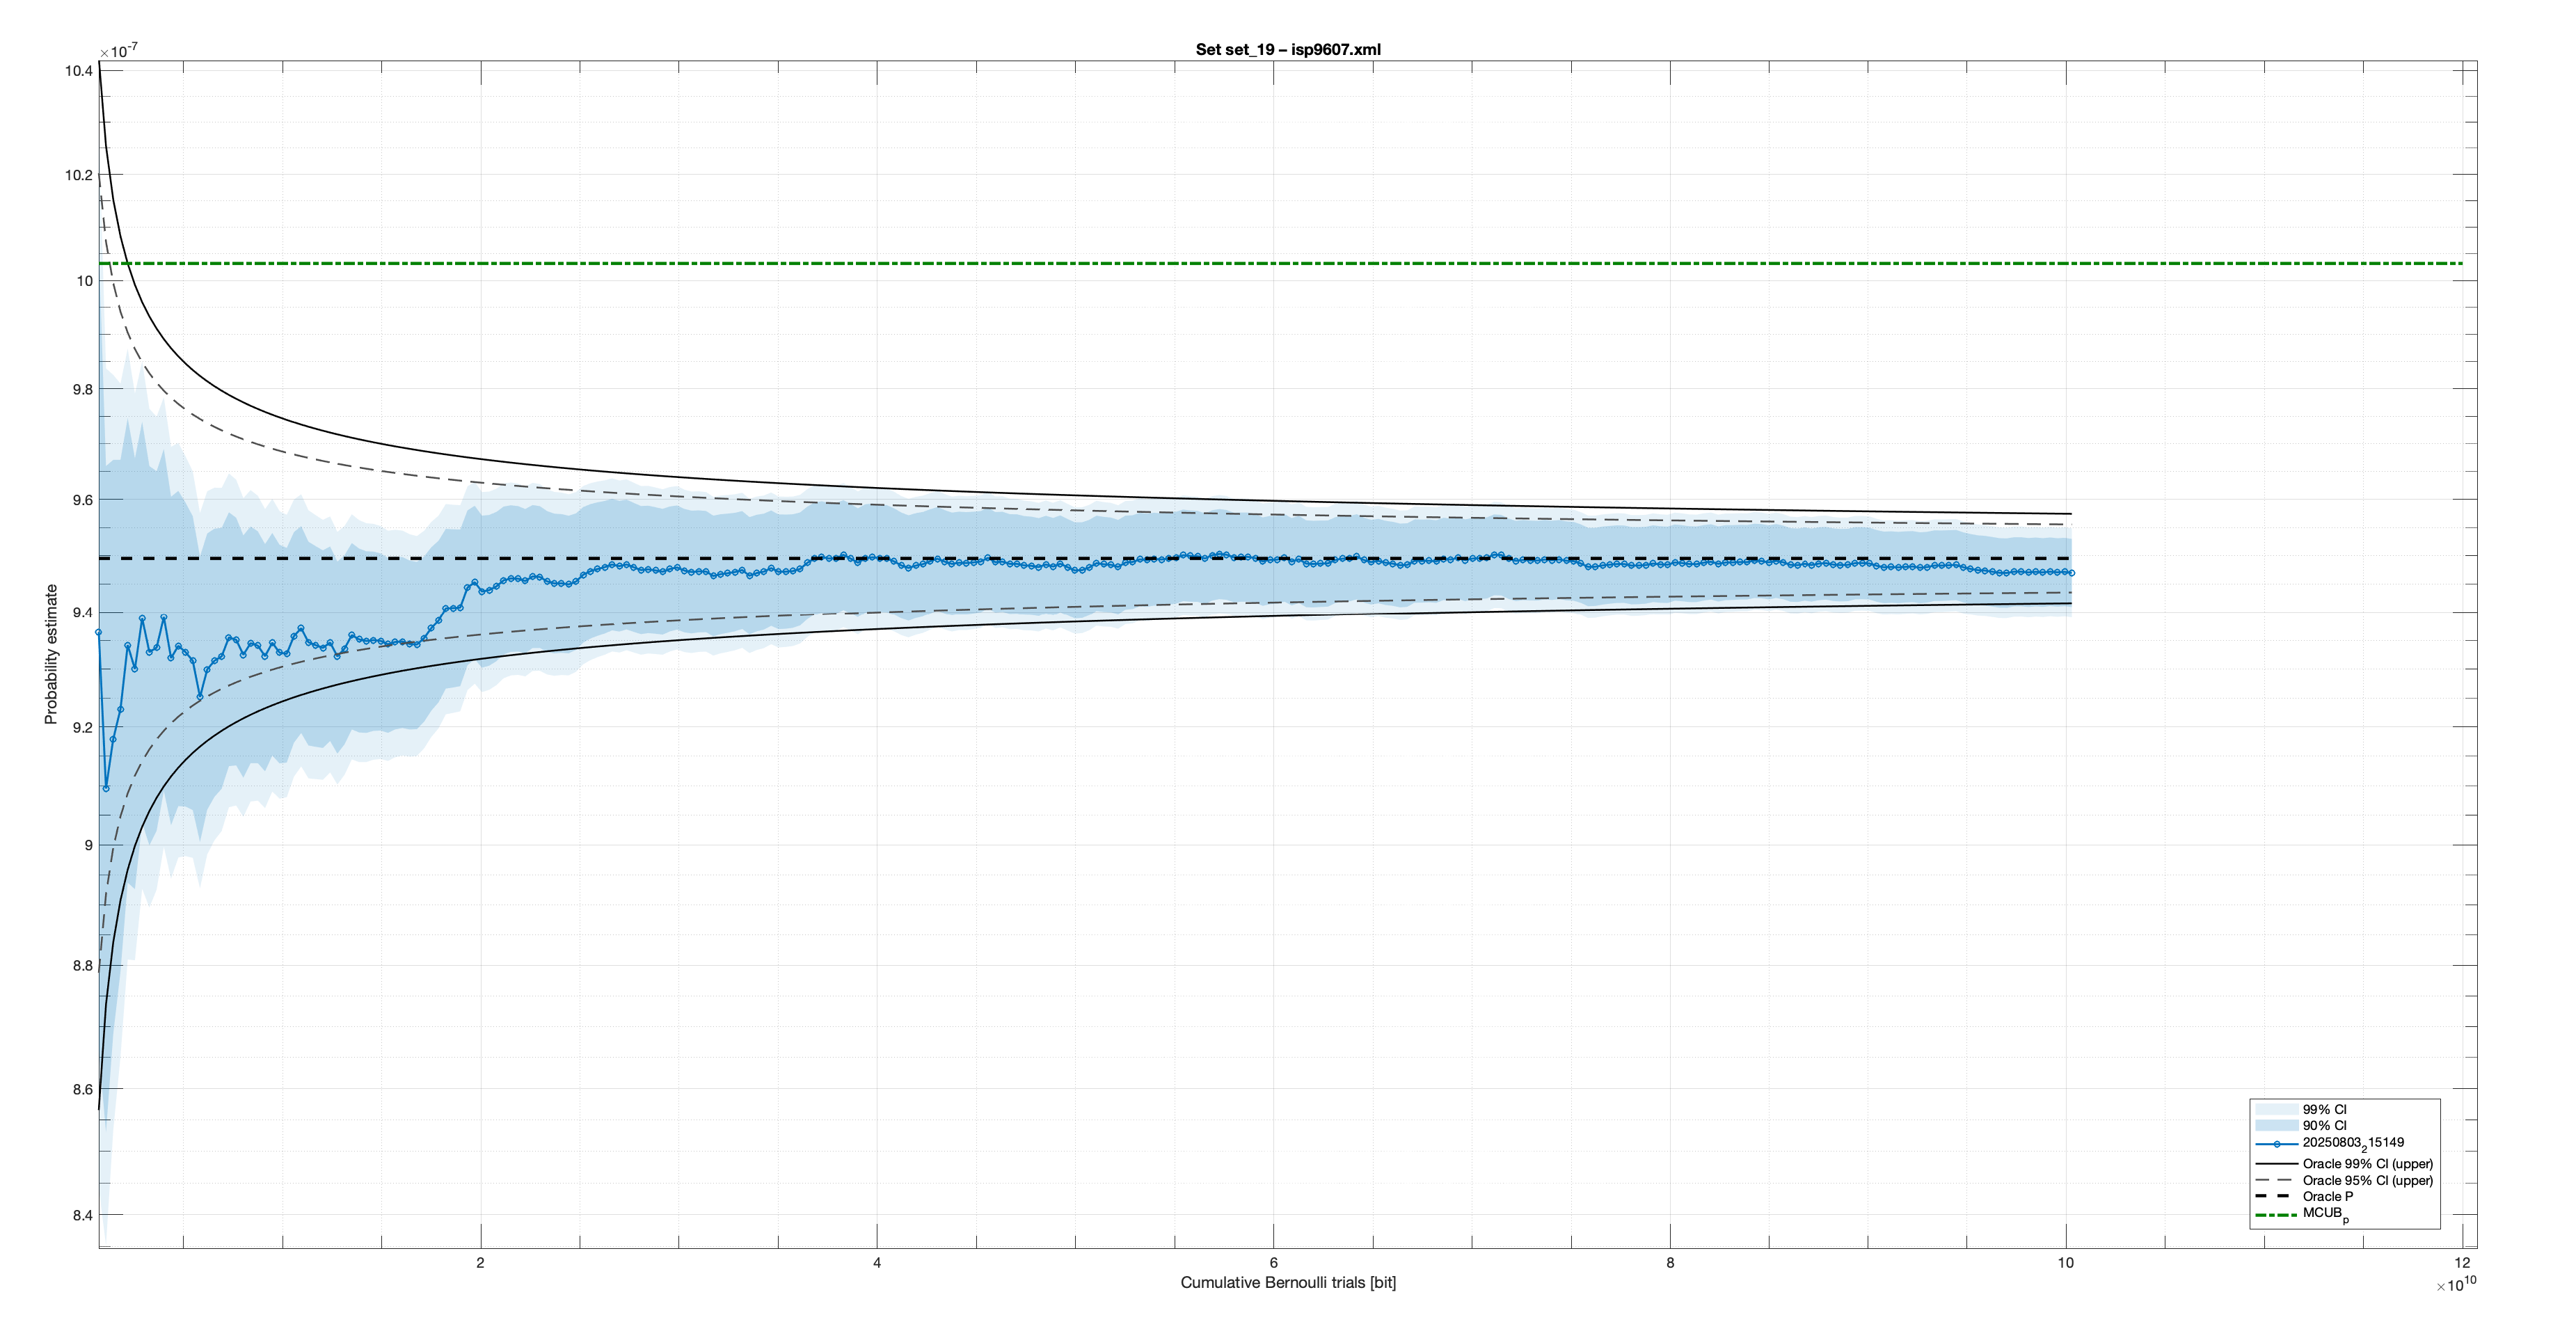
\includegraphics[height=0.9\textheight]{4_casestudy/conv_ips9607.eps}
    \label{fig:convergence_run_01}
\end{figure}
\end{frame}

\subsection{Convergence Free Run}
\begin{frame}
    \begin{figure}[h]
    \centering
    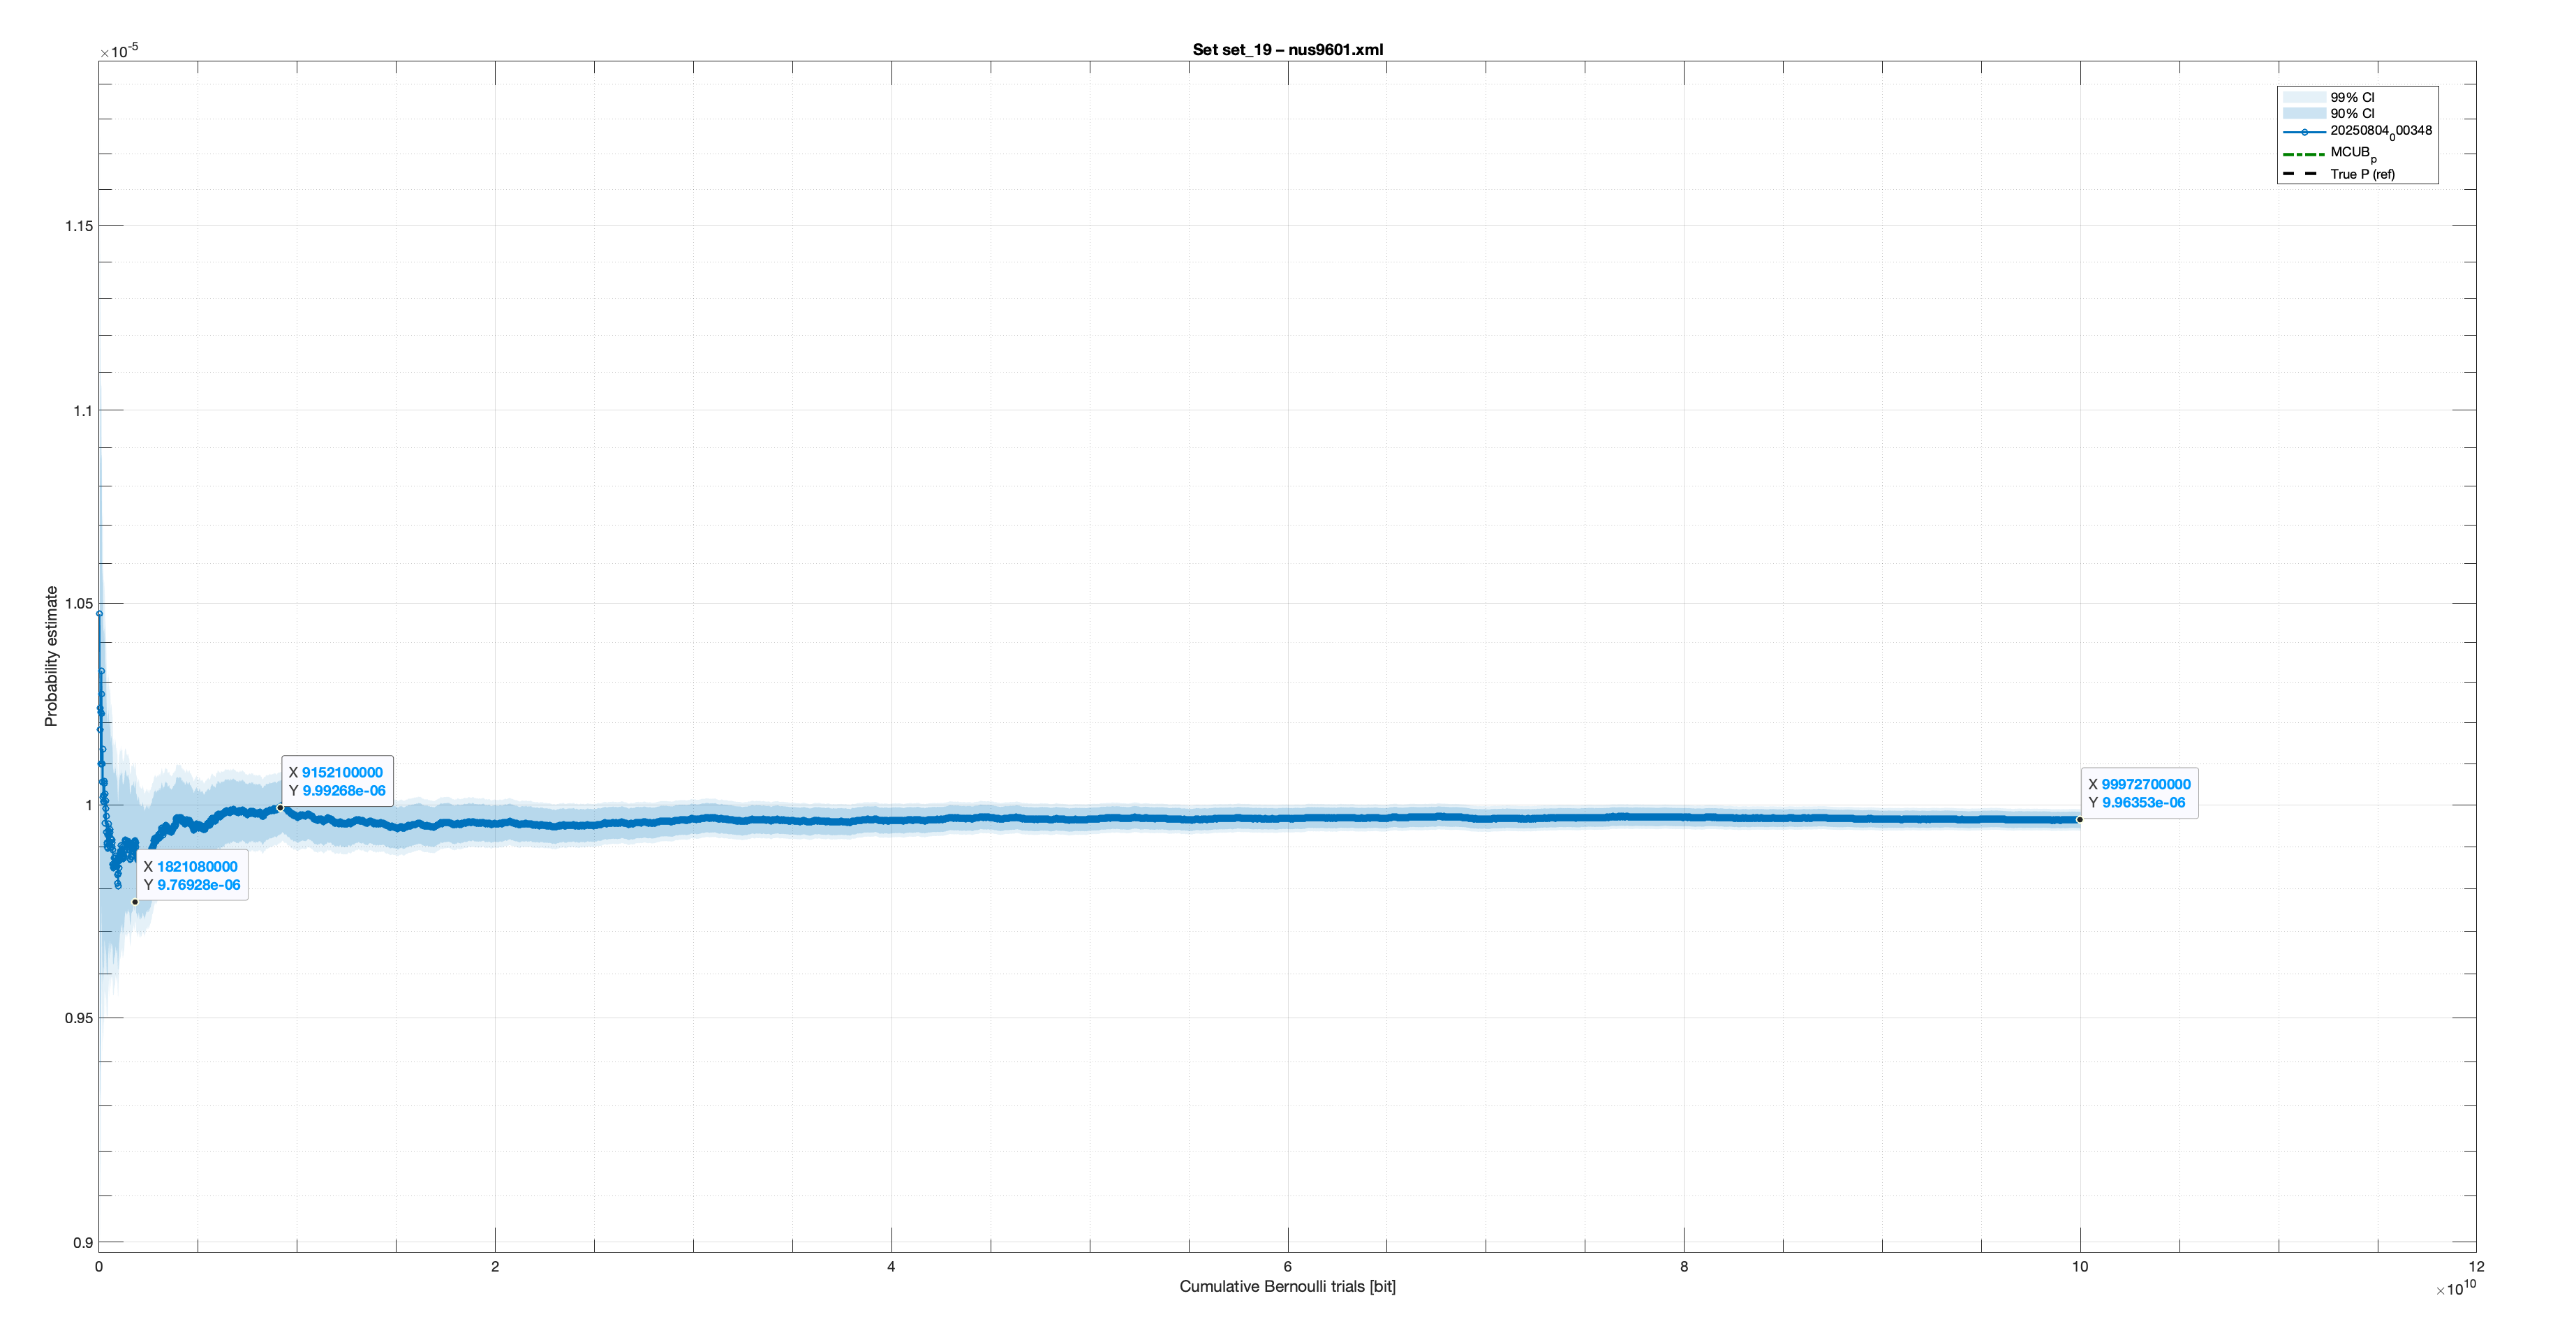
\includegraphics[width=1\textwidth]{4_casestudy/conv_nus9601.eps}
    \label{fig:rare}
\end{figure}
\end{frame}


\subsection{Aralia Fault Tree Data Set - Convergence for Rare Events}
\begin{frame}
    \input{4_casestudy/4_mae}
\end{frame}

% \subsection{Aralia Fault Tree Data Set - Throughput Benchmarks}
% \begin{frame}
%     \begin{figure}[h]
%     \centering
%     \includegraphics[width=0.9\textwidth]{4_casestudy/throughput/slides_nodes_vs_throughput.eps}
%     \caption{PDAG Node Count vs Throughput [bit/s]}
%     \label{fig:nodes_vs_throughput}
% \end{figure}
% \end{frame}




% \begin{frame}{Aralia Fault Tree Dataset}
% show the input dataset table\\
% \end{frame}

% \subsection{Results}
% \begin{frame}{Mar}
% show the input dataset table\\
% \end{frame}


\input{2_framework/research_objective_6_domain/importance_measures}

\input{2_framework/research_objective_6_domain/ccf}

\section{Research Objective 5: Case Studies and Benchmarks}
\begin{frame}
    \Large{\centerline{\textbf{Research Objective 5}}}
    \vspace{6pt}
    \large{\centerline{\textbf{Case Studies and Benchmarks}}}
\end{frame}

\subsection{Aralia Fault Tree Data Set}
\begin{frame}[t]
\frametitle{Overview: Aralia Dataset}
\begin{itemize}
  \item \textbf{Dataset Composition:} The Aralia collection consists of 43 distinct fault trees, each with varying numbers of basic events (BEs), gate types (AND, OR, K/N, XOR), and minimal cut-set counts.  
  \item \textbf{Diverse Problem Sizes:} Small trees (e.g.\ 25--32 BEs) through large models with over 1{,}500 BEs.  
  \item \textbf{Wide Probability Range:} Top-event probabilities spanning from rare events near \(10^{-13}\) to fairly likely failures with probability above 0.7.  
  \item \textbf{Model Variability:} Some trees are primarily AND/OR, others incorporate more advanced gates (K/N, XOR, NOT), providing thorough coverage of typical (and atypical) fault tree logic structures.
\end{itemize}
\end{frame}

\begin{frame}[allowframebreaks]
    \input{4_casestudy/3_table_aralia_ft_dataset}
\end{frame}

\subsection{Benchmarking Procedure}
\begin{frame}[t]
\frametitle{Benchmarking Setup: Hardware and Environment}
\begin{itemize}
  \item \textbf{Target Hardware:}
    \begin{itemize}
      \item GPU: NVIDIA\textsuperscript{\textregistered} GeForce GTX 1660 SUPER (6\,GB GDDR6, 1{,}408 CUDA cores).
      \item CPU: Intel\textsuperscript{\textregistered} Core\textsuperscript{TM} i7-10700 (2.90\,GHz, turbo-boost, hyperthreading).
    \end{itemize}
  \item \textbf{Software Stack:}
    \begin{itemize}
      \item SYCL-based (AdaptiveCpp/HipSYCL), with LLVM-IR JIT for kernel compilation.
      \item Compiler optimization at \texttt{-O3} for efficient code generation.
      \item Repeated runs (5+) to mitigate transient variations.
    \end{itemize}
  \item \textbf{Measured Time:} Includes entire wall-clock duration, from host-device transfers and JIT compilation to final result collection.
\end{itemize}
\end{frame}

\subsection{Accuracy Benchmarks}
\begin{frame}
    \begin{figure}[h]
    \centering
    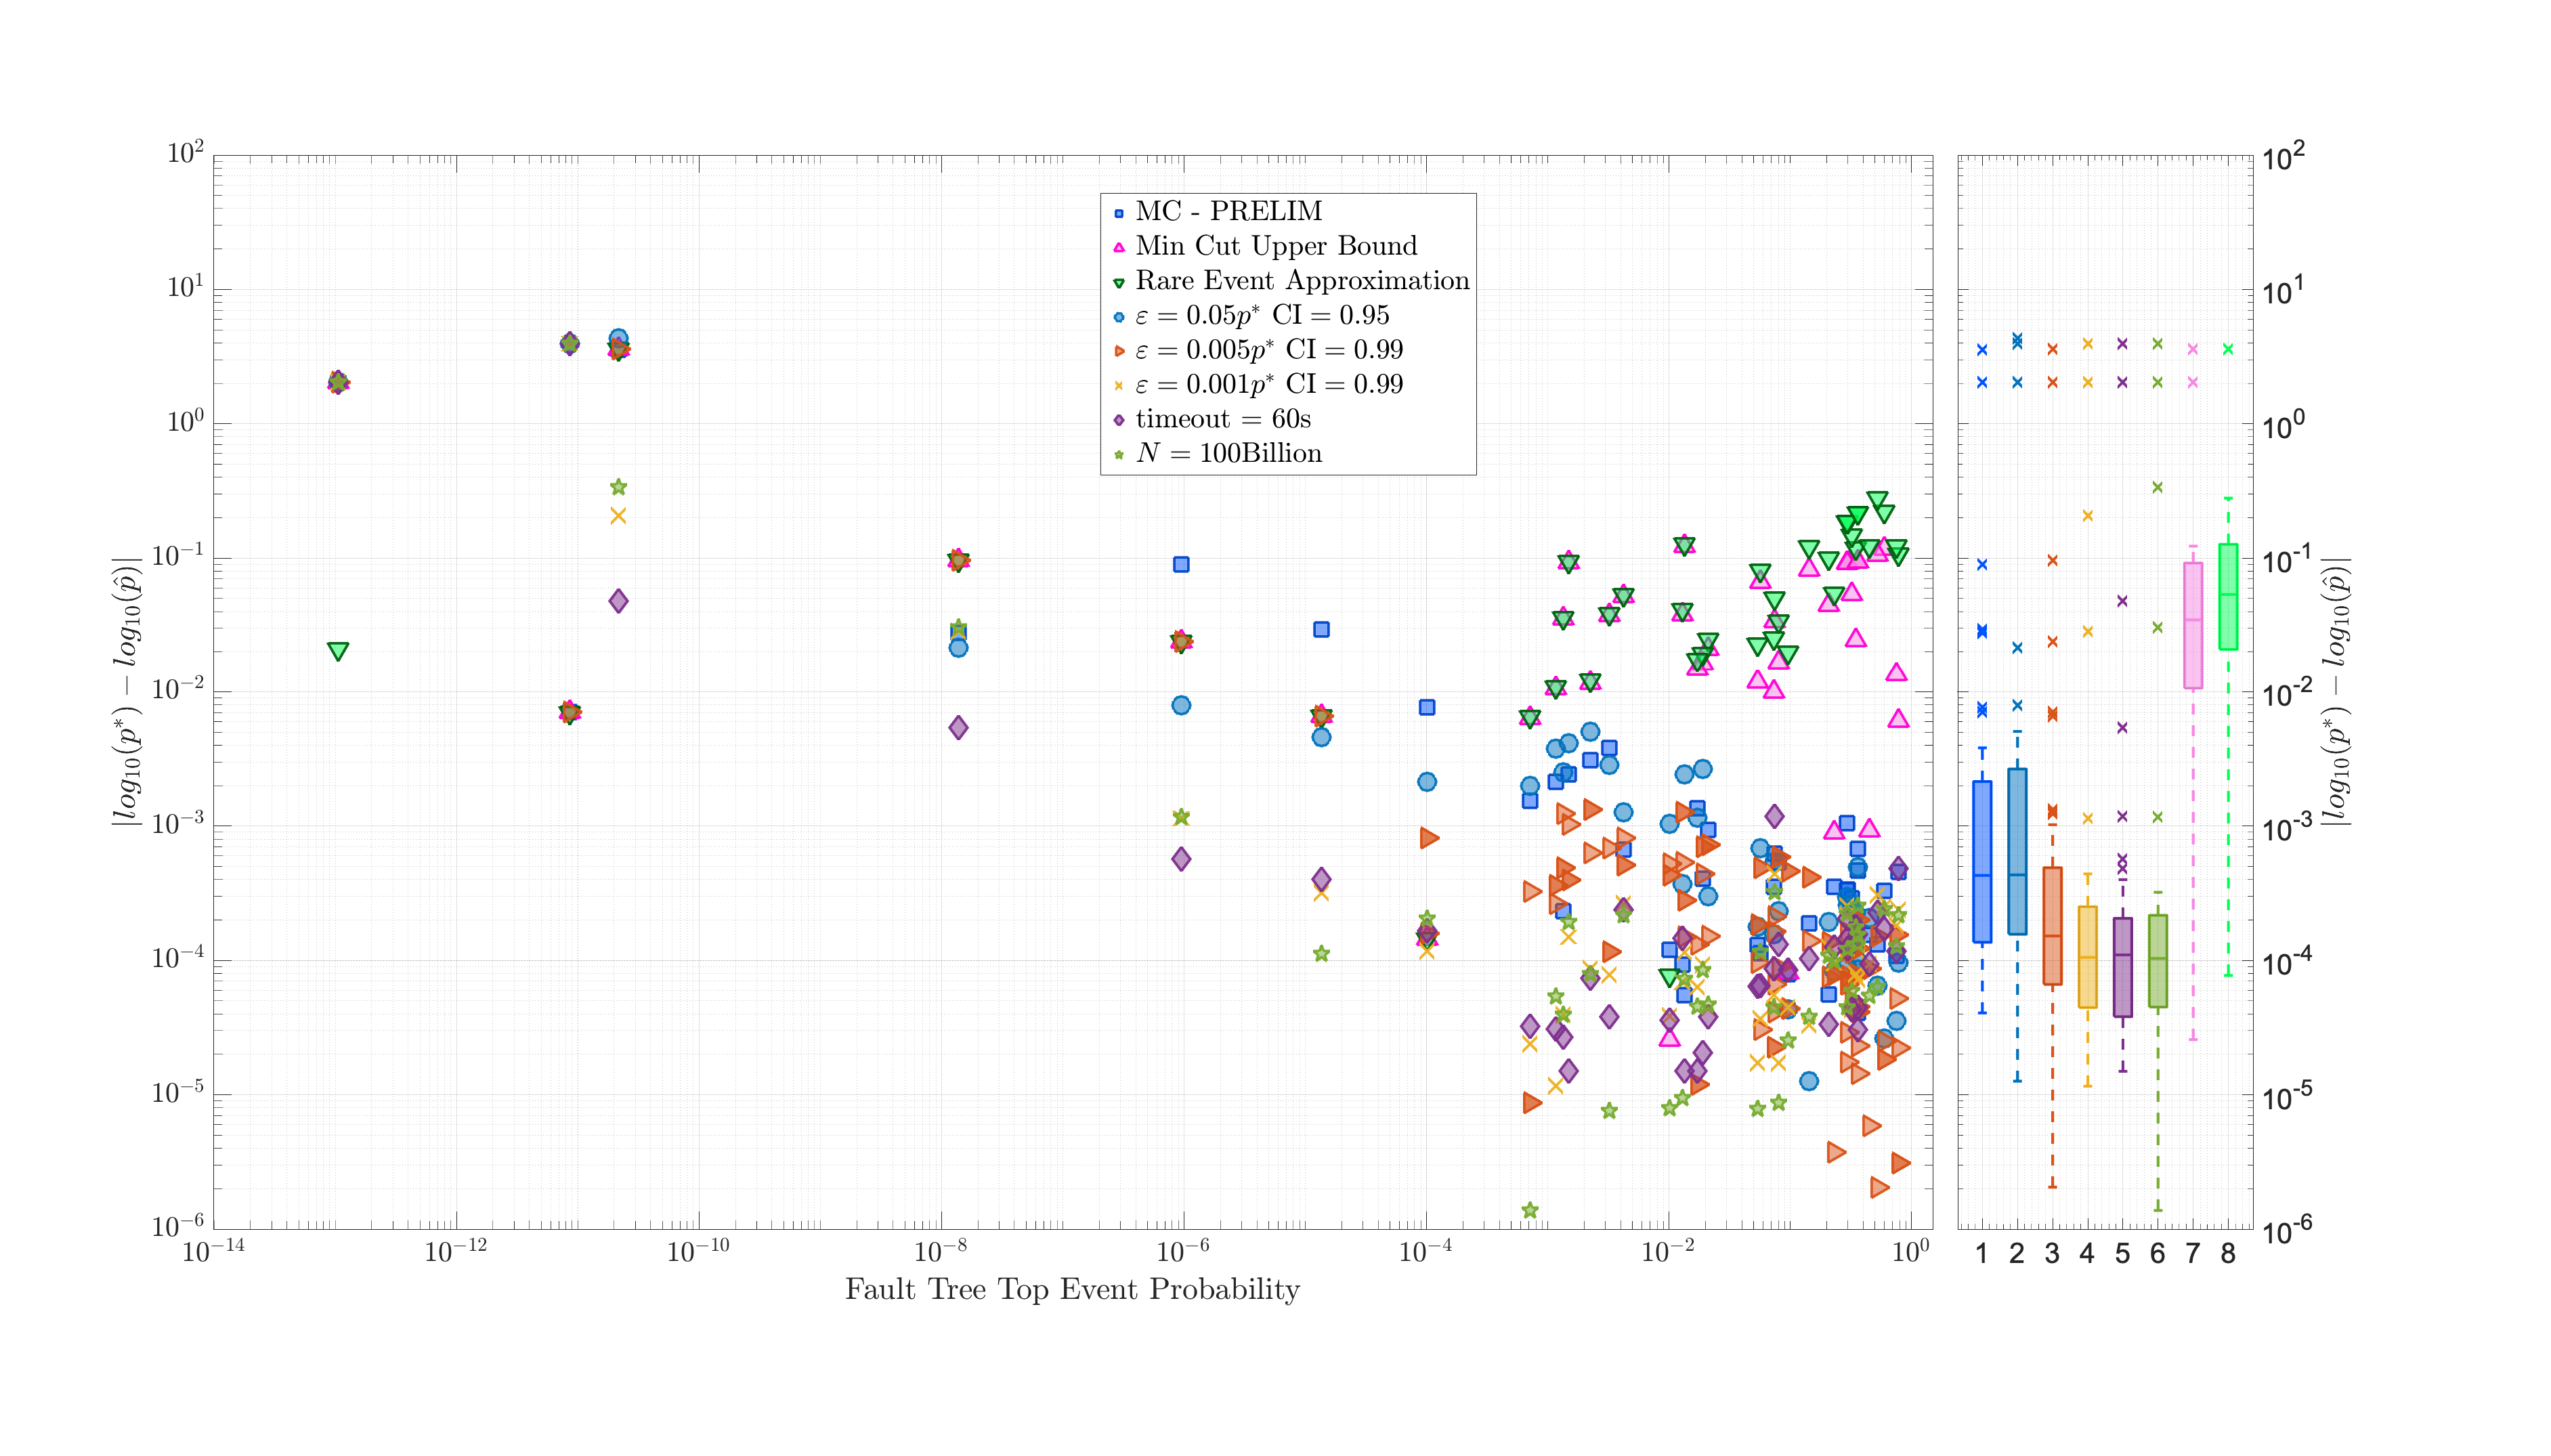
\includegraphics[height=1.1\textheight]{4_casestudy/abs_err.eps}
    \label{fig:mae_vs_logp}
\end{figure}
\end{frame}

\subsection{Accuracy vs. Time to Convergence}
\begin{frame}
\begin{figure}[p]
    \centering
    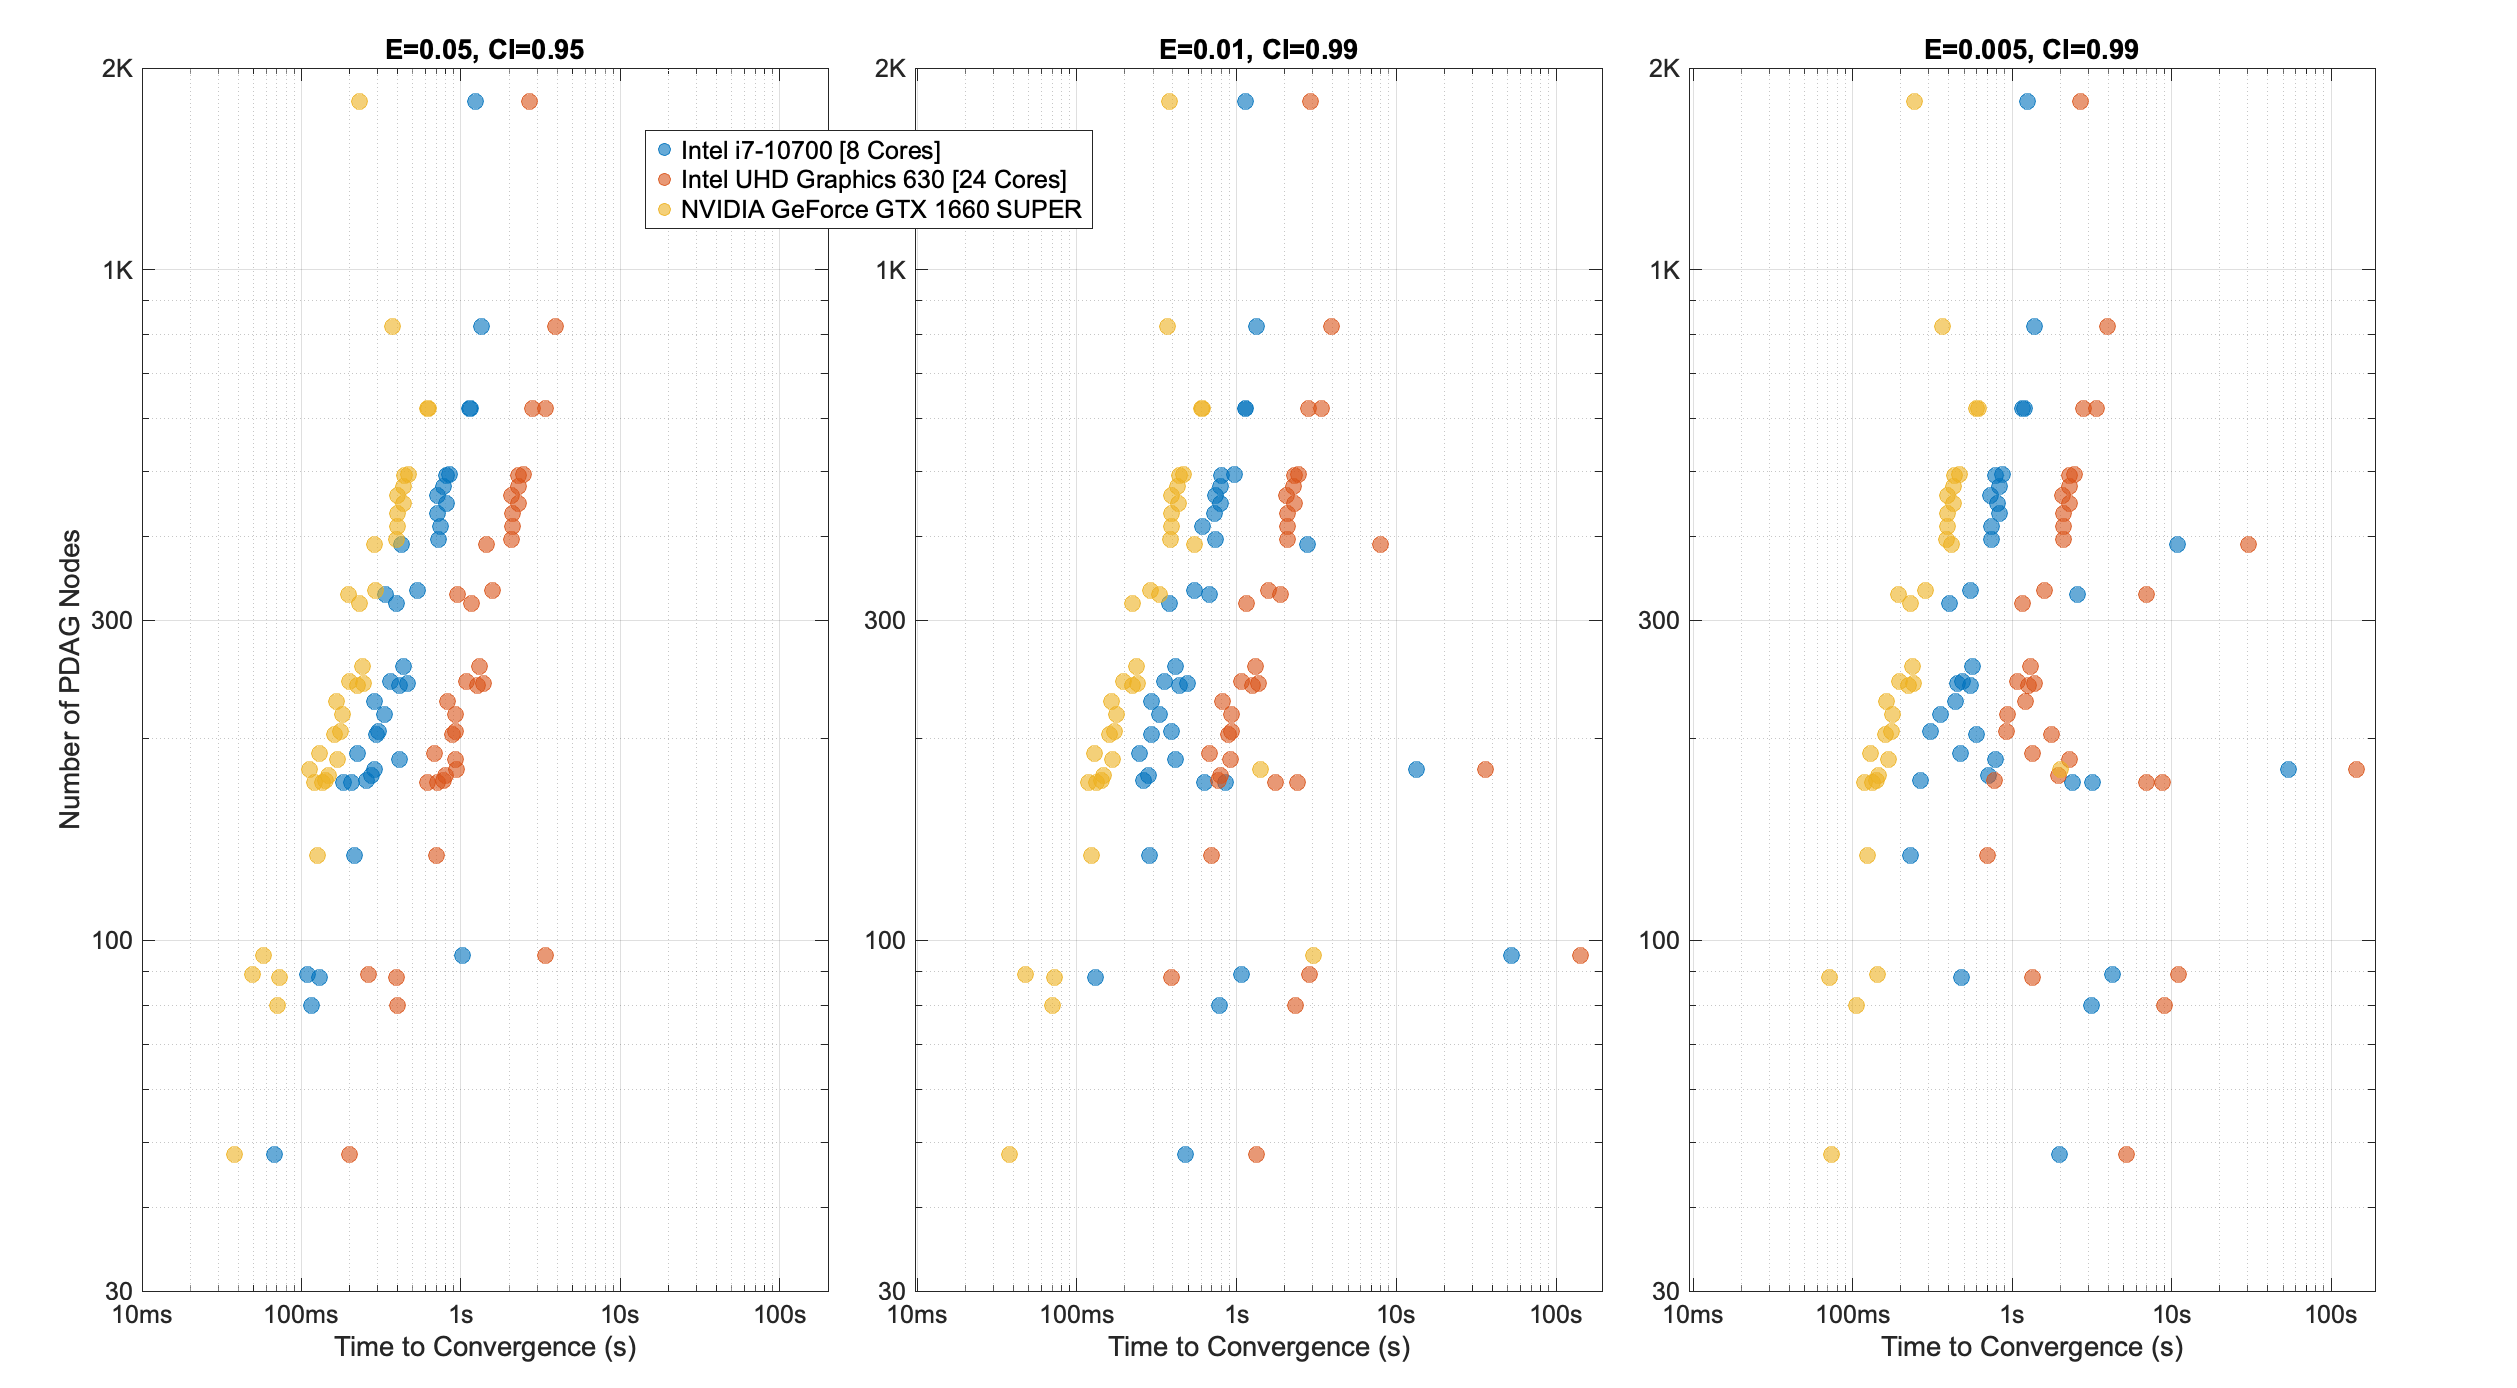
\includegraphics[height=1\textheight]{4_casestudy/throughput/slides_nodes_vs_convergence.eps}
    \caption{Time to convergence for different accuracy targets.}
    \label{fig:nodes_vs_convergence}
\end{figure}
\end{frame}

\subsection{Convergence Runs}
\begin{frame}
\begin{figure}[p]
    \centering
    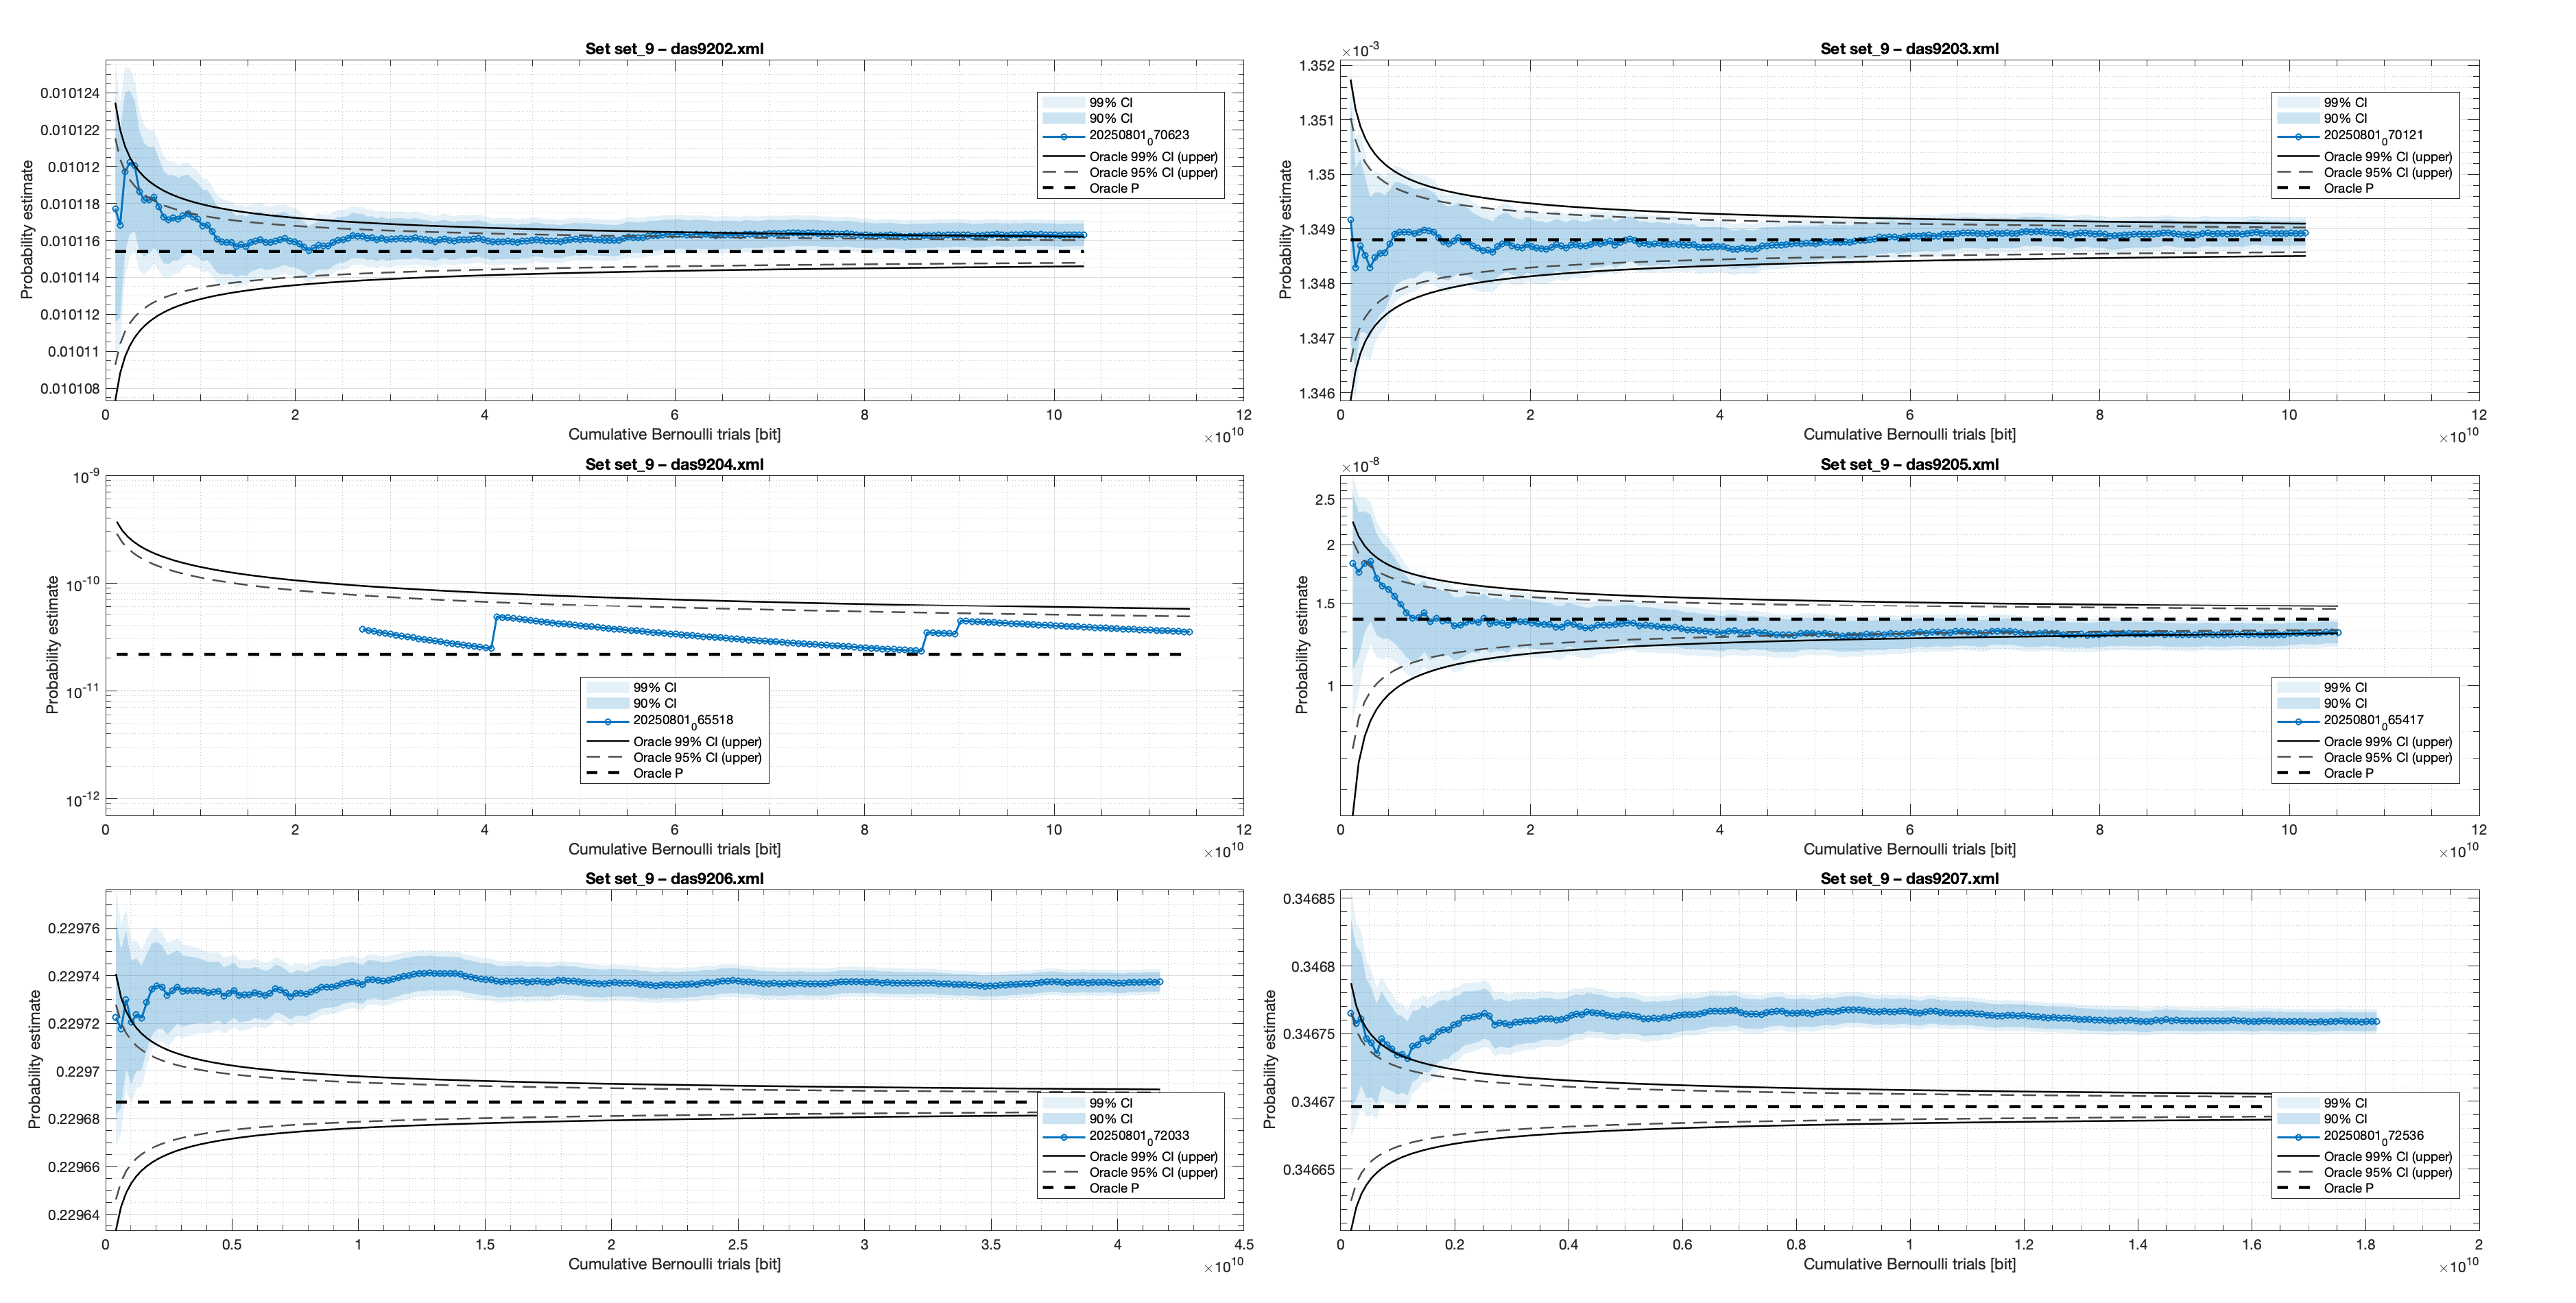
\includegraphics[height=1\textheight]{4_casestudy/conv_raw.eps}
    \label{fig:convergence_run_01}
\end{figure}
\end{frame}

\subsection{Convergence Runs, Comparison with MCUB, REA}
\begin{frame}
\begin{figure}[p]
    \centering
    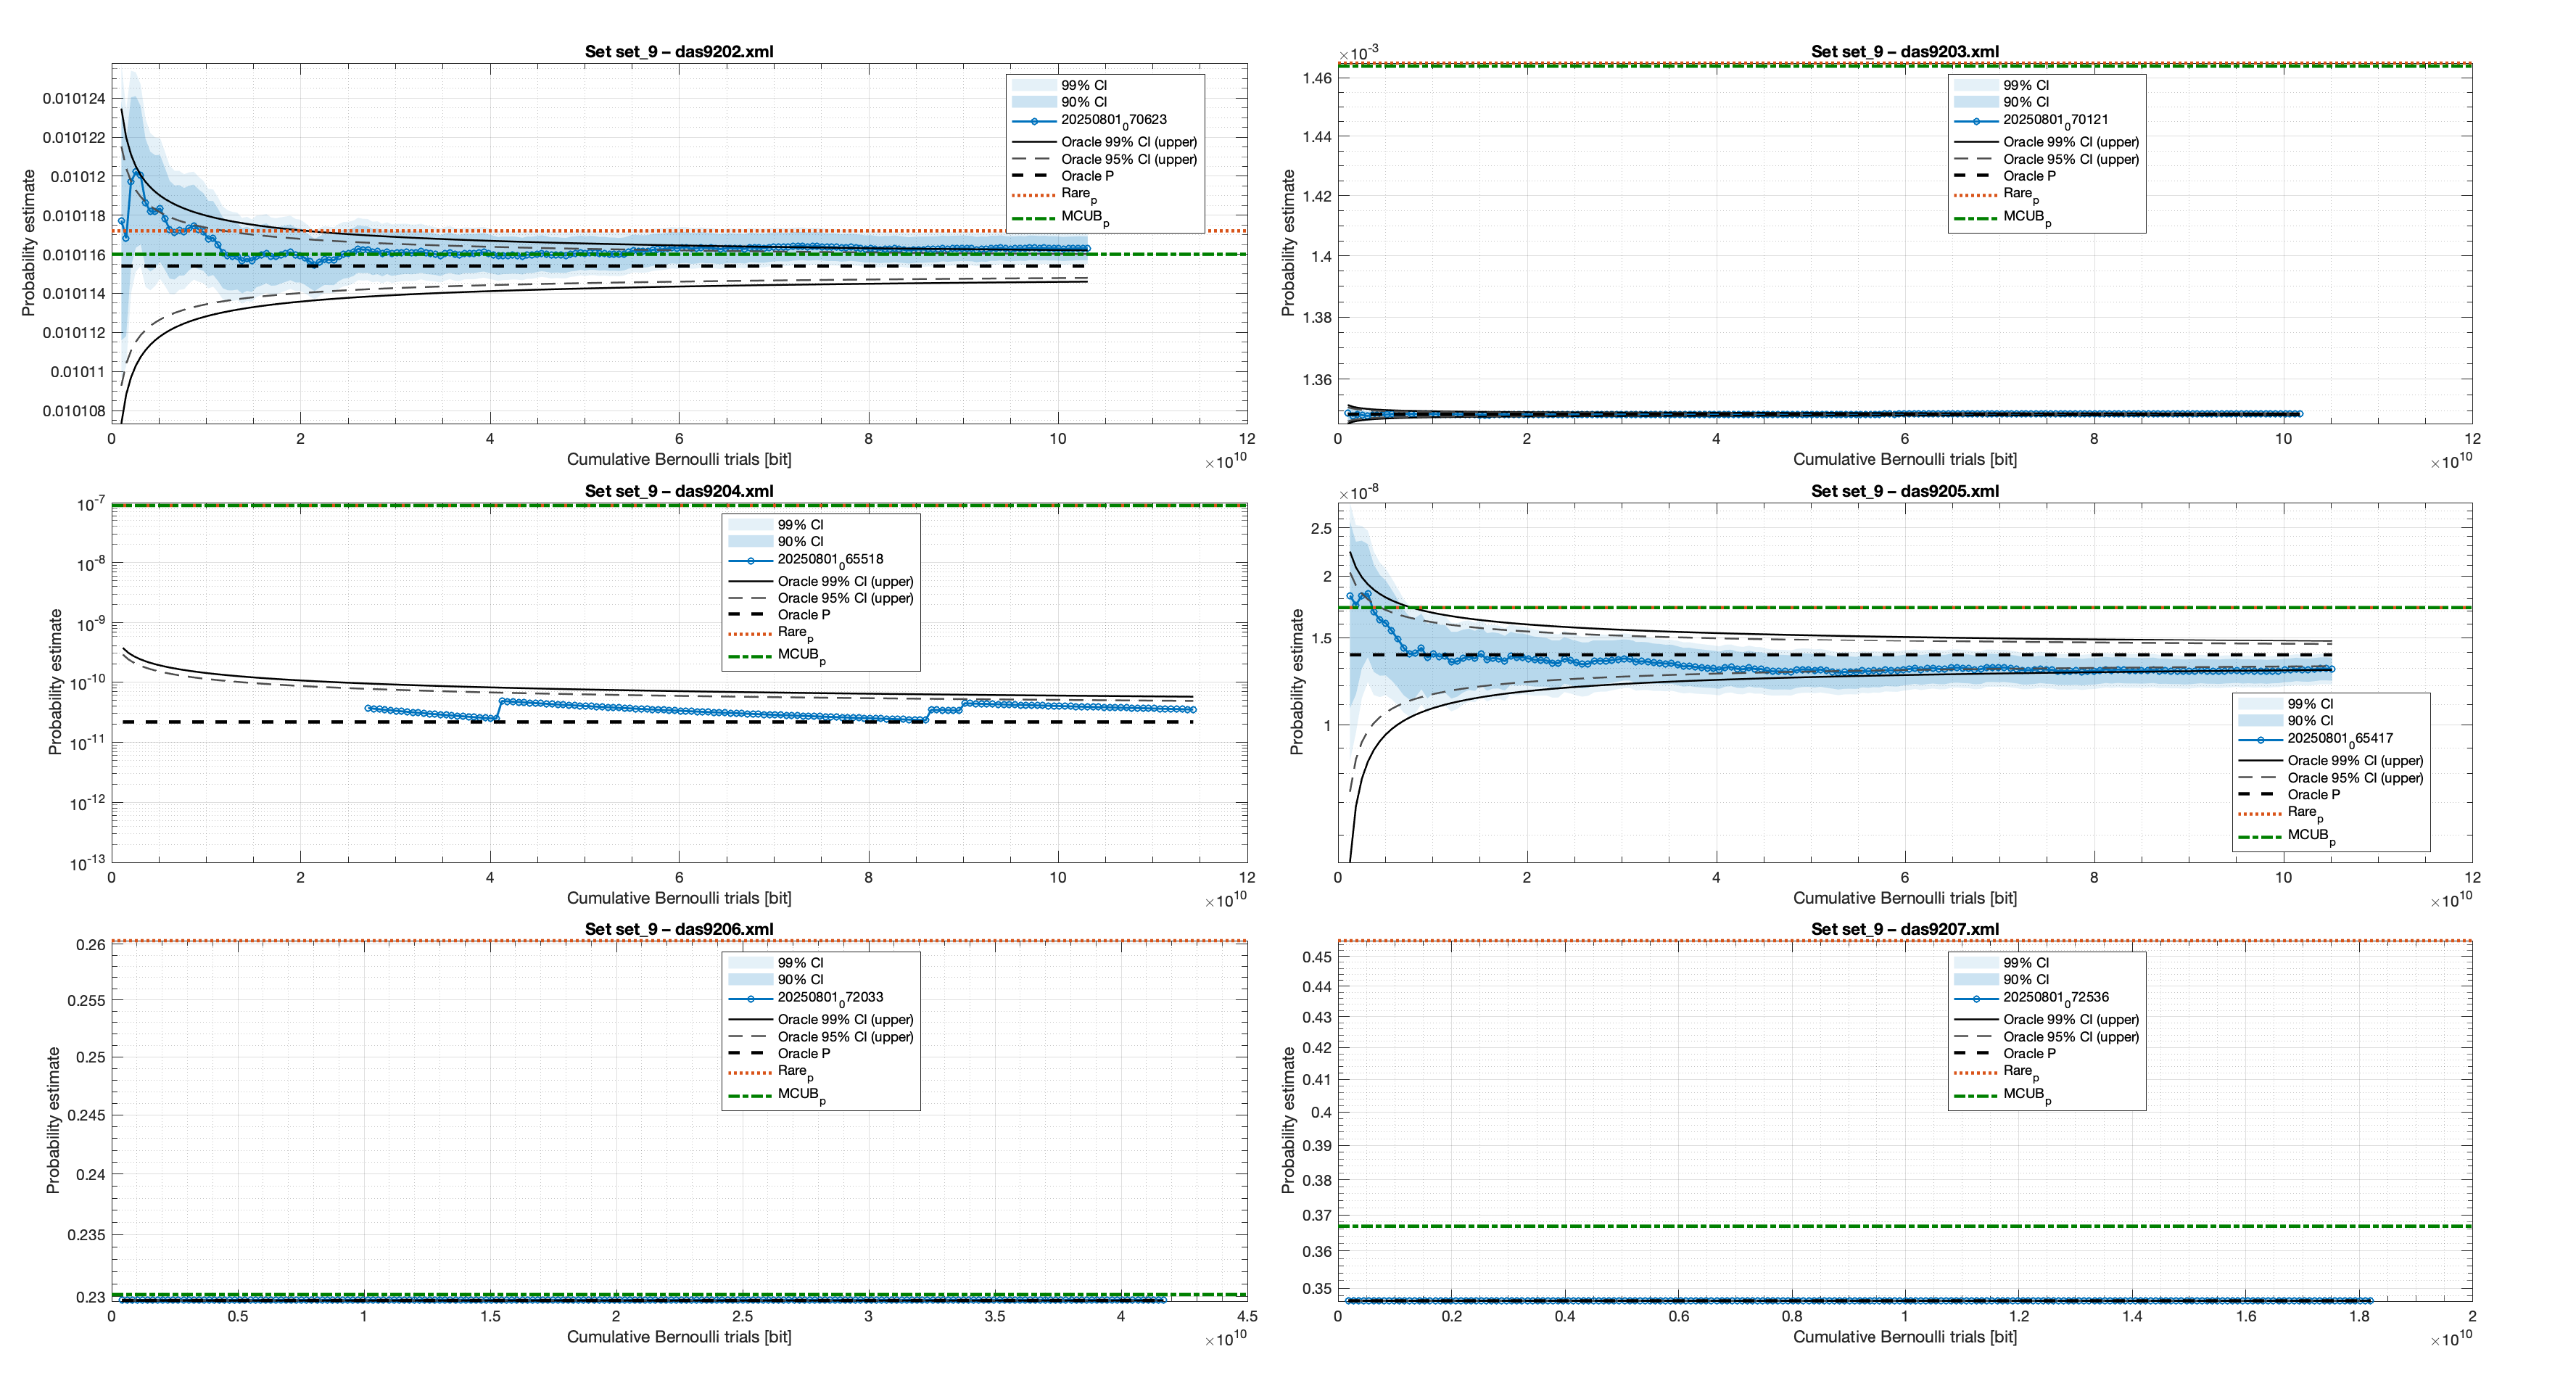
\includegraphics[height=1\textheight]{4_casestudy/conv_figeps.eps}
    \label{fig:convergence_run_01}
\end{figure}
\end{frame}

\subsection{Convergence Run -- Rare Event, Comparison with MCUB}
\begin{frame}
\begin{figure}[p]
    \centering
    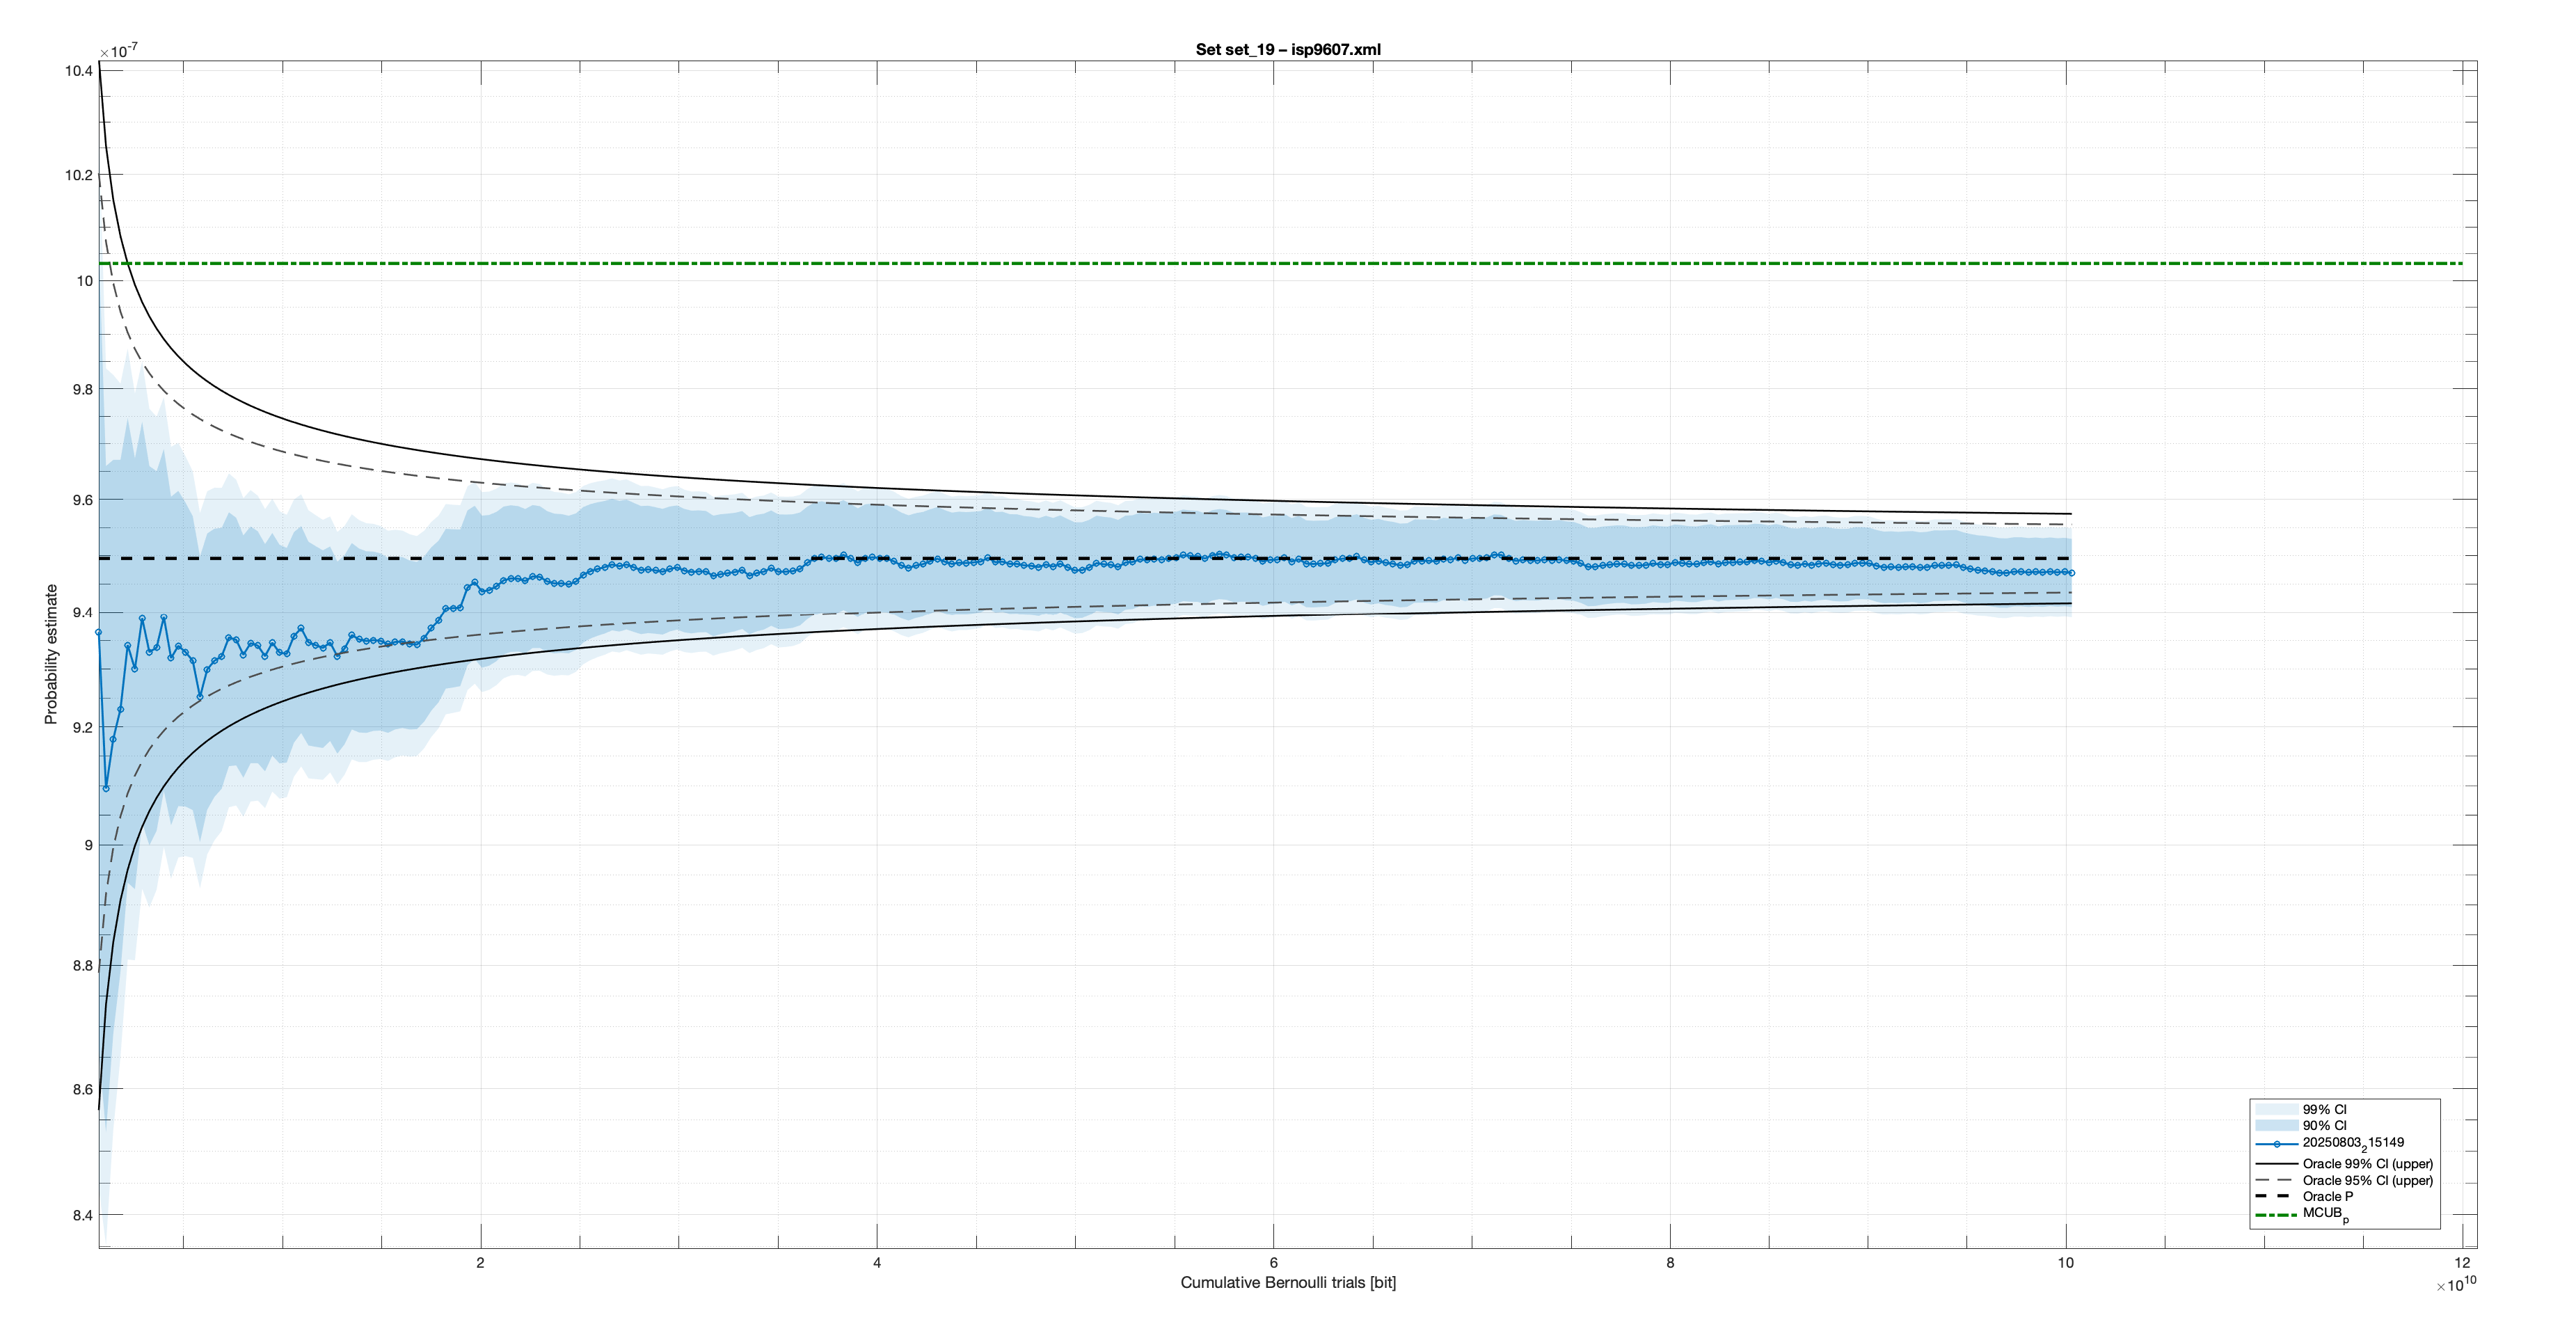
\includegraphics[height=0.9\textheight]{4_casestudy/conv_ips9607.eps}
    \label{fig:convergence_run_01}
\end{figure}
\end{frame}

\subsection{Convergence Free Run}
\begin{frame}
    \begin{figure}[h]
    \centering
    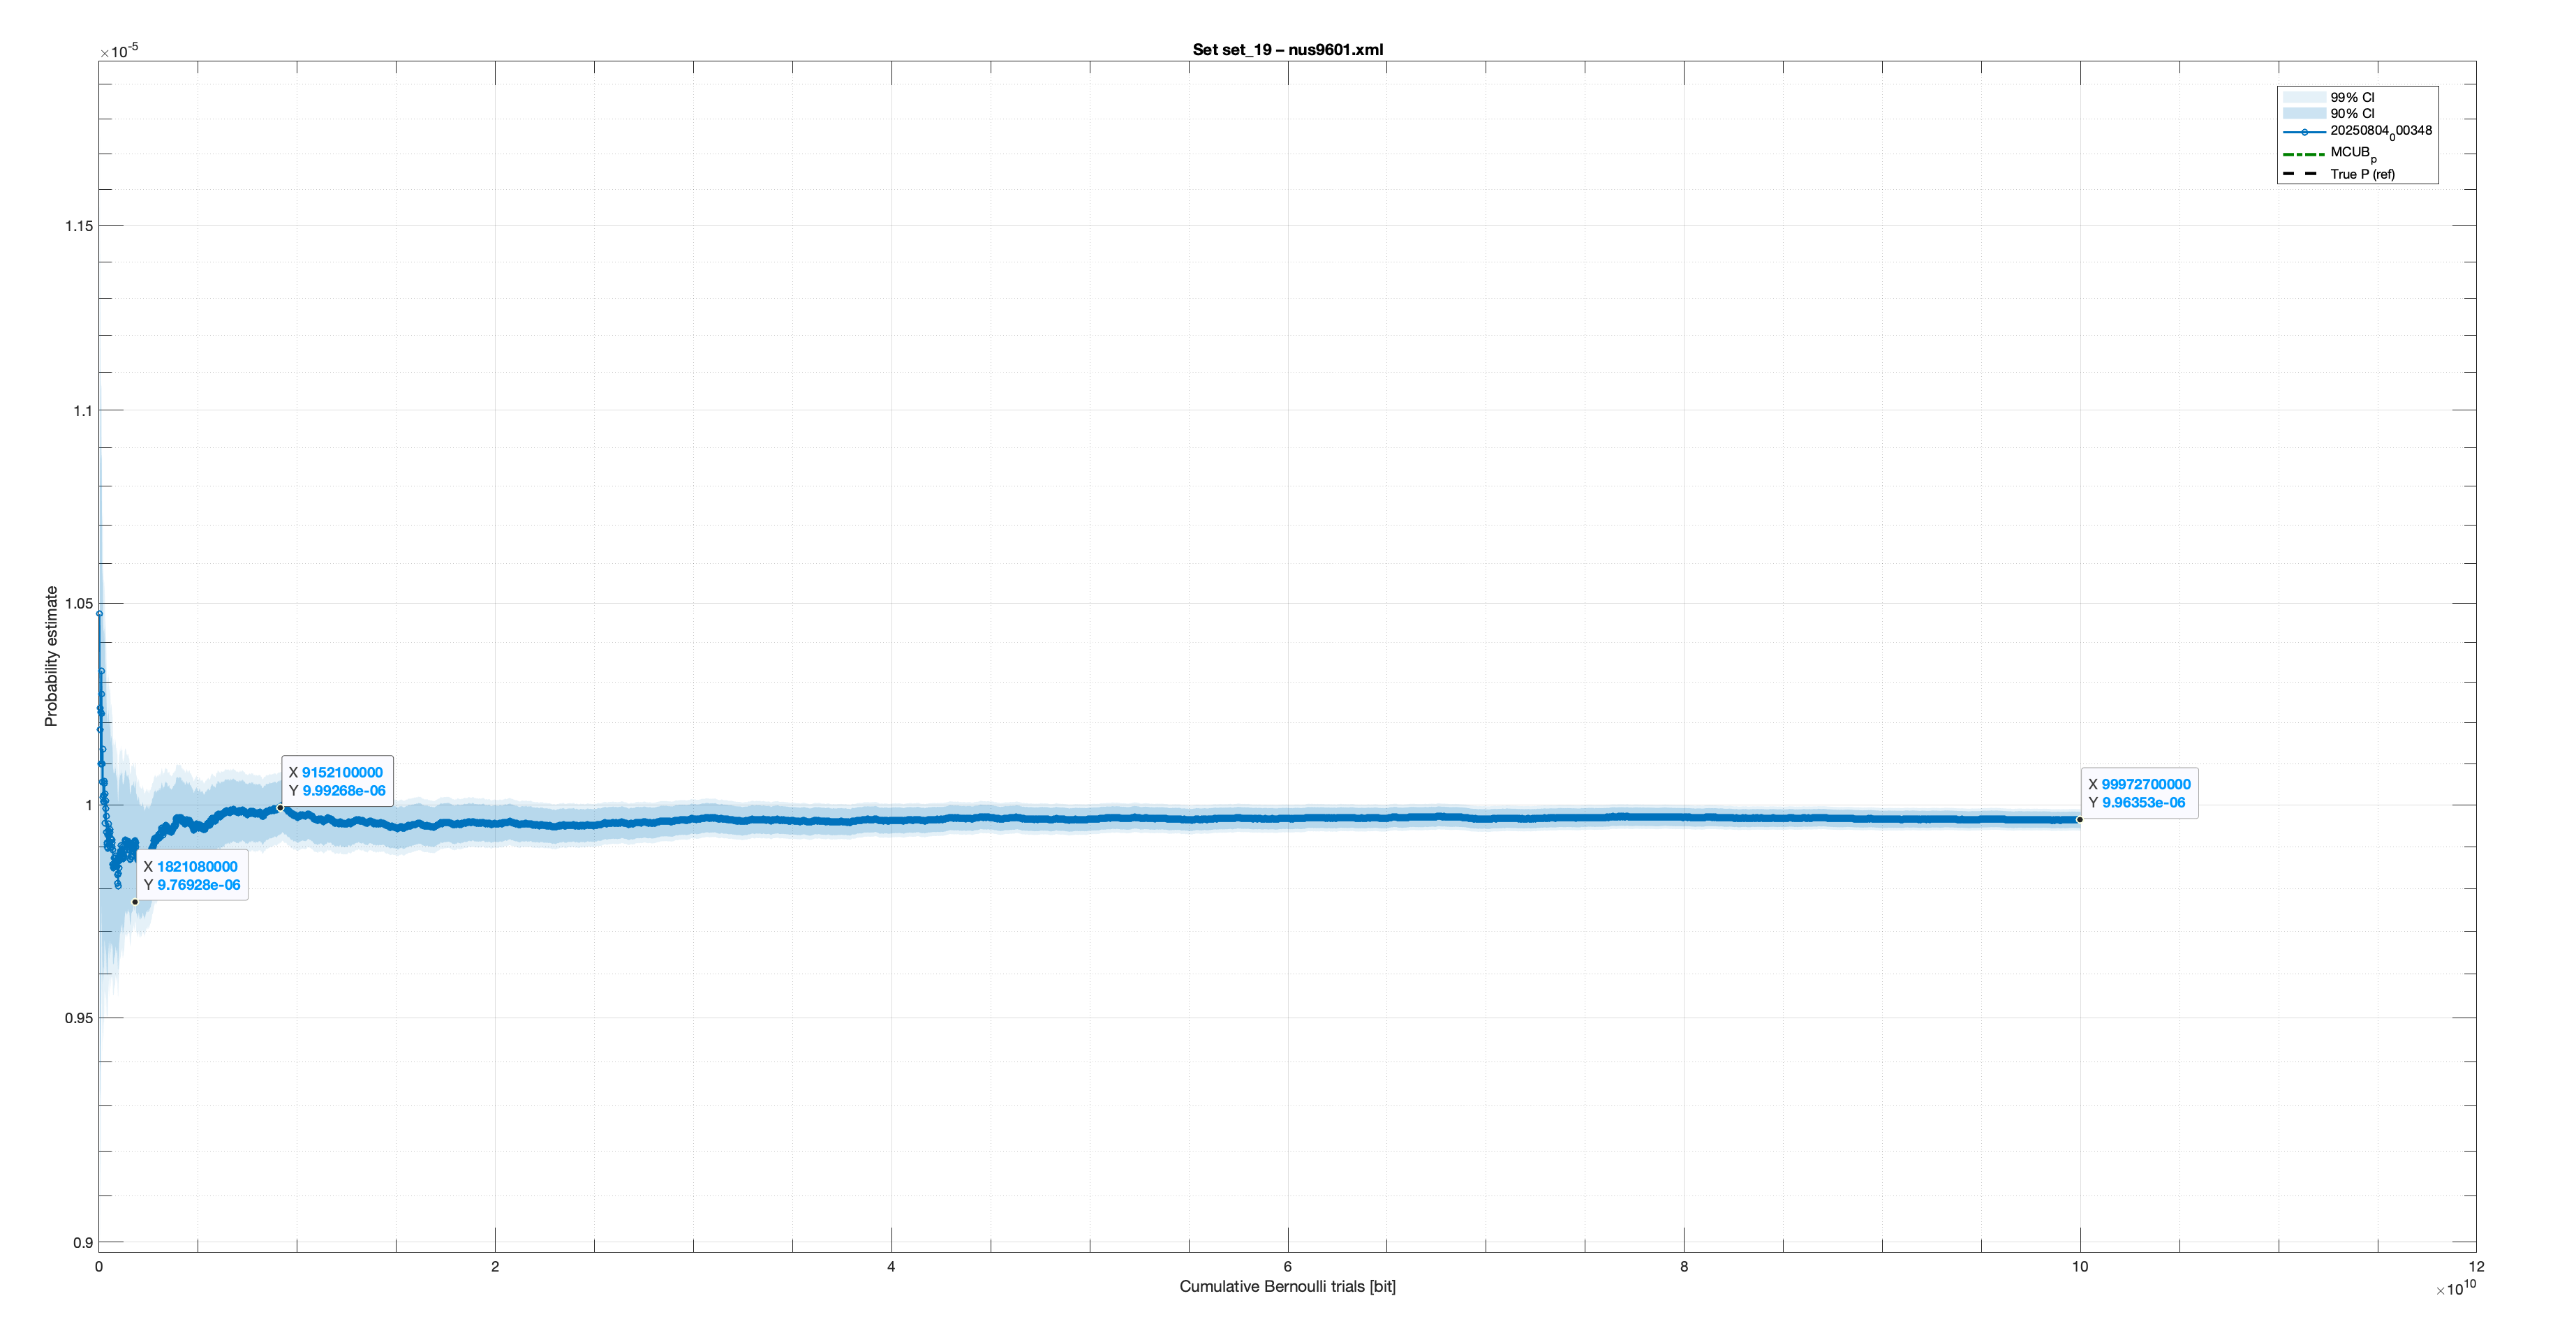
\includegraphics[width=1\textwidth]{4_casestudy/conv_nus9601.eps}
    \label{fig:rare}
\end{figure}
\end{frame}


\subsection{Aralia Fault Tree Data Set - Convergence for Rare Events}
\begin{frame}
    \input{4_casestudy/4_mae}
\end{frame}

% \subsection{Aralia Fault Tree Data Set - Throughput Benchmarks}
% \begin{frame}
%     \begin{figure}[h]
%     \centering
%     \includegraphics[width=0.9\textwidth]{4_casestudy/throughput/slides_nodes_vs_throughput.eps}
%     \caption{PDAG Node Count vs Throughput [bit/s]}
%     \label{fig:nodes_vs_throughput}
% \end{figure}
% \end{frame}




% \begin{frame}{Aralia Fault Tree Dataset}
% show the input dataset table\\
% \end{frame}

% \subsection{Results}
% \begin{frame}{Mar}
% show the input dataset table\\
% \end{frame}
% With the objective of bridging the gap between PDAG and probabilistic circuits, generate a section, including multiple frames, that (1) introduce the concept of the triplet definition of risk, (2) scenario modeling in PRA,  (3) event trees, (4) fault trees, (5) event tree / fault tree linking (together as a PRA model), (6) the concept of a PDAG, (7) PRA model as a PDAG. So, include at-least 7 frames, but you can use more. Include equations and definitions where appropriate.

\section{Research Objective 1: Bridge PRA Modeling Semantics with Probabilistic Circuits}
\begin{frame}
    \Large{\centerline{\textbf{Research Objective 1}}}
    \vspace{6pt}
    \large{\centerline{\textbf{Bridge PRA Modeling Semantics with Probabilistic Circuits}}}
\end{frame}

\subsection{PRA Overview}
\begin{frame}[allowframebreaks]
\frametitle{The Triplet Definition of Risk}
\begin{itemize}
  \item Define risk as a set of triplets, each representing:
    \begin{enumerate}
      \item What can go wrong? (\(S_i\))
      \item How likely is it to happen? (\(L_i\))
      \item What are the consequences? (\(X_i\))
    \end{enumerate}
        \vspace{6pt}
  \item
    \begin{equation}
    \label{eq:risk_triplets_slides}
      R \;=\;\bigl\{\langle S_i,\,L_i,\,X_i\rangle\bigr\}_{c},
    \end{equation}
    \(\,c\) represents completeness in enumerating \emph{all} relevant scenarios.
\end{itemize}
\end{frame}

\begin{frame}[allowframebreaks]
\frametitle{Scenario \(S_i\) Modeling in PRA}
\begin{itemize}
  \item Each scenario unfolds from initiating events (IEs), followed by conditional branching events.
          \vspace{6pt}
  \item Fundamental goal: assign probabilities to these scenarios {and} assess resulting outcomes (e.g., core damage, large release).
          \vspace{6pt}
  \item Implementation typically uses structured diagrams such as:
    \begin{itemize}
      \item Event Trees (ETs): forward chaining from IE to various end states.
      \item Fault Trees (FTs): top-down decomposition to basic events (component failures).
    \end{itemize}
\end{itemize}
\end{frame}

\begin{frame}[t, allowframebreaks]
\frametitle{Event Trees}
\begin{figure}[ht!]
\centering
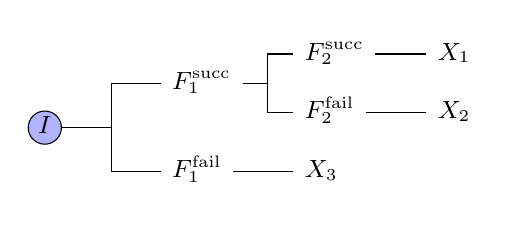
\begin{tikzpicture}
\tikzset{grow'=right,level distance=48pt}
\tikzset{execute at begin node=\strut}
\tikzset{every tree node/.style={anchor=base west}}
\tikzset{
    edge from parent/.append style={very thick},
    edge from parent/.style={
        draw,
        edge from parent path={
            (\tikzparentnode.east) -| ($(\tikzparentnode.east)!0.5!(\tikzchildnode.west)$) |- (\tikzchildnode.west)
        },
    },
    every node/.style={anchor=center,font=\small\bfseries, text centered, inner sep=0pt},
    every level 0 node/.style={circle, font=\small\bfseries, draw, fill=blue!30, inner sep=0pt},
    every internal node/.style={font=\small, inner sep=4pt},
    every leaf node/.style={rectangle, draw, fill=blue!30, minimum width=2.5cm, text centered},
    frontier/.style={distance from root=400pt},
}
\Tree [.\(I\)
    [.\(F_1^{\text{succ}}\)
        [.\(F_2^{\text{succ}}\)
            [.\(X_1\) ]
        ]
        [.\(F_2^{\text{fail}}\)
            [.\(X_2\) ]
        ]
    ]
    [.\(F_1^{\text{fail}}\)
        [.\(X_3\) ]
    ]
]
\end{tikzpicture}
\caption{Illustrative event tree with an initiating event \(I\), two functional events \(F_1\) and \(F_2\), and three end-states \(X_1, X_2, X_3\).}
\label{fig:event_tree_example}
\end{figure}
\begin{itemize}
  \item An Event Tree represents how an initiating event \(I\) can branch into multiple functional-event outcomes.
  \item Each functional event \(F_k\) may succeed or fail, driving the path toward a distinct end-state \(X_j\).  
  \item If \(\omega_j\) denotes one branch leading to \(X_j\), then the branch probability often factors as 
    \[
      p(\omega_j) \;=\; p(I)\;\times\;\prod_{k=1}^{n} \; p\bigl(F_k^{\alpha_k} \;\mid\; \text{all previous outcomes}\bigr).
    \]
  \item As a logical expression, each \(\omega_j\) translates to an AND of success/failure literals, and the overall set of end-states is an OR of these branches:
    \[
      \Omega \;=\;\omega_1 \;\lor\;\omega_2 \;\lor\;\dots\;\lor\;\omega_m.
    \]
  \item Consequently, ETs are in \emph{sum of products} (SOP) or \emph{disjunctive normal form} (DNF), where each product term identifies one success/failure path and the scenario-level outcome is the logical OR across all such paths.
  \vspace{4pt}
  \item Graphically straightforward, but can combinatorially expand for deep branching.
\end{itemize}
\end{frame}

\begin{frame}[t, allowframebreaks]
\frametitle{Fault Trees}
    \begin{figure}[h]
    \centering
    \includegraphics[width=0.5\textwidth]{1_concepts/ft.png}
    \caption{Fault tree with 6 basic events, top event $X = (a_1\bigwedge b_1) \bigvee (a_2\bigwedge b_2) \bigvee (a_3\bigwedge b_3)$}
    \label{fig:ft}
\end{figure}
\begin{itemize}
  \item A Fault Tree describes how a top event (system failure) can result from lower-level component or subsystem failures.
  \item Internal gates (AND, OR, \(k\)-of-\(n\), etc.) combine events in logical fashion:
    \[
      \text{Output} \;=\;
      \begin{cases}
         \bigwedge_{i=1}^k e_i, & \text{(AND)}\\
         \bigvee_{i=1}^k e_i, & \text{(OR)}\\
         \dots
      \end{cases}
    \]
  \item Basic events (BEs) in the leaves have assigned probabilities \(p(b)\).  Independence often assumed unless modeling common-cause failures.
  \item The top event failure probability can be written as:
    \begin{equation}
    \label{eq:top_event_probability_slides}
    \Pr[\text{Top Fail}] \;=\; \sum_{S \subseteq \,\mathcal{B}} 
      \Bigl[
        \pi_{F}(S, \text{Top}) 
        \prod_{b\in S} p(b)\prod_{b\notin S}[1 - p(b)]
      \Bigr].
    \end{equation}
\end{itemize}
\end{frame}

\begin{frame}[t, allowframebreaks]
\frametitle{Linking Event Trees and Fault Trees in PRA}
\begin{itemize}
  \item Real systems often combine:
    \begin{itemize}
      \item Forward branching dynamics via Event Trees (ET).
      \item Subsystem or component reliability logic via Fault Trees (FT).
    \end{itemize}
  \item An event tree branch may call a specific FT top event to collect system failure or success.
  \item Conversely, a fault tree output may feed back into an event tree branch as an initiating event or functional node outcome.
  \item This multi-level interconnection \(\implies\) a need for a unified model capturing both forward branching (ET) and hierarchical failure logic (FT).
\end{itemize}
\end{frame}

\begin{frame}[t, allowframebreaks]
\frametitle{Probabilistic Directed Acyclic Graph (PDAG)}
\begin{itemize}
  \item A PDAG is a Directed Acyclic Graph whose edges carry either:
    \begin{itemize}
      \item Conditional probabilities (e.g., for event tree branches).  
      \item Logical dependencies (e.g., for fault tree gates).
    \end{itemize}
  \item Nodes may include:
    \begin{itemize}
      \item Basic events (BEs) with known probabilities.
      \item ET or FT intermediate events storing partial results.
      \item Any top-level node (e.g., a final end-state) with no children.
    \end{itemize}
  \item The absence of cycles guarantees consistent flow from initial seeds (basic events, initiating events) to final outcomes.
  \item PDAG forms the structural backbone for bridging scenario-based expansions with gate-based logic in a single coherent representation.
\end{itemize}
\end{frame}

\subsection{Probabilistic Circuits Overview}
\begin{frame}[t, allowframebreaks]
\frametitle{Probabilistic Circuits: A Brief Overview}
    \begin{figure}[h]
    \centering
    \includegraphics[height=0.5\textheight]{1_concepts/pc.png}
    \caption{Probabilistic circuit with 4 inputs $X_i$, product gates (blue), sum gate (orange)}
    \label{fig:pc}
\end{figure}
\end{frame}

\begin{frame}[t, allowframebreaks]
\begin{itemize}
  \item A \textbf{probabilistic circuit} is a directed acyclic graph (DAG) that encodes a joint probability distribution through \emph{sum-gates} and \emph{product-gates}.
  \item \textbf{Sum-gates} approximate mixture distributions:
    \[
      p_v(\mathbf{x})
      \;=\;
      \sum_{u\in \operatorname{ch}(v)} \theta_{v,u}\,p_u(\mathbf{x}),
      \quad
      \text{with }
      \sum_{u\in \operatorname{ch}(v)} \theta_{v,u} = 1.
    \]
    Each child distribution is weighted by a nonnegative parameter \(\theta_{v,u}\).
  \item \textbf{Product-gates} factorize independent variable sets:
    \[
      p_v(\mathbf{x})
      \;=\;
      \prod_{u\in \operatorname{ch}(v)} p_u\bigl(\mathbf{x}_{u}\bigr),
    \]
    assuming disjoint subsets of variables for each child \(u\).
  \item \textbf{Leaf nodes} (inputs) often correspond to known base distributions. When evaluated upward through the DAG, each internal node yields its own distribution, culminating in a root node that represents the full model.
  \item \textbf{Key motivation}:
    \begin{itemize}
      \item Tractable inference: evaluation and certain marginal or conditional queries can be performed in time proportional to circuit size.  
      \item Decomposability and modularity: separate, interpretable substructures that can be reused or combined for large-scale systems.
    \end{itemize}
\end{itemize}
\end{frame}

\subsection{PRA PDAGs to Probabilistic Circuits}
\begin{frame}[allowframebreaks]
\frametitle{Compiled PRA Graphs are PDAGs}
\begin{itemize}
  \item A unified PRA model can be viewed as
    \[
      \mathcal{M} 
      \;=\;
      \langle 
        \mathcal{V},\,\mathcal{A},\, \{p(b)\},\, \{\theta_{u\to v}\},\,\pi_{F}
      \rangle,
    \]
    where \(\mathcal{V}\) includes basic events, ET nodes, and FT gates, and \(\mathcal{A}\) is the acyclic edge set.
  \item Event-tree edges carry transitional probabilities \(\theta_{u\to v}\) summing to 1 from each node.
  \item Fault-tree nodes embed Boolean logic \(\pi_F\) that checks if inputs fail under a subset of basic events.
  \framebreak
  \item This PDAG perspective:
    \begin{itemize}
      \item Ensures systematic accounting of all scenario paths and subsystem logic.
      \item Aligns naturally with tractable Probabilistic Circuits, since each node’s distribution/function can be embedded in a sum-product style DAG.
      \item Offers a foundation for efficient Monte Carlo or advanced inference methods.
    \end{itemize}
    \vspace{6pt}
    \item Ongoing work to bridge PRA PDAG semantics with Probabilistic Circuits:
    \begin{itemize}
      \item PDAGs can be transformed to equivalent canonical forms (there are tradeoffs).
    \end{itemize}
\end{itemize}
\end{frame}
% % !TeX TS-program = lualatex
%----------------------------------------------------------------------------------------
%    PACKAGES AND THEMES
%----------------------------------------------------------------------------------------

\documentclass[aspectratio=169,xcolor=dvipsnames]{beamer}
\usetheme{SimpleDarkBlue}

\usepackage{booktabs}  % professionally typeset tables
\usepackage{amsmath}
\usepackage{amsthm}
\usepackage{amssymb} 
\usepackage{amsfonts}
\usepackage{tikz}
\usepackage{tikz-qtree}
\usetikzlibrary{calc,positioning}
\usepackage{pgfpages}
% \setbeameroption{show notes on second screen}

\usepackage{textcomp}  % better copyright sign, among other things
\usepackage{lipsum}    % filler text
\usepackage{lscape}
\usepackage{longtable}
\usepackage{siunitx}
% Please add the following required packages to your document preamble:
\usepackage{multirow}
\usepackage[table,xcdraw]{xcolor}
\usepackage{xstring}
\usepackage{relsize}
\usepackage{hyperref}
\usepackage{graphicx} % Allows including images
\usepackage{fontspec}
%\usepackage{helvet}
\setsansfont{Open Sans}
%----------------------------------------------------------------------------------------
%    TITLE PAGE
%----------------------------------------------------------------------------------------

\title{A Data-Parallel Monte Carlo Framework for Large-Scale PRA
using Probabilistic Circuits}
\subtitle{Preliminary Exam}

\author{Arjun Earthperson}

\institute
{
    Department of Nuclear Engineering \\
    North Carolina State University % Your institution for the title page
}
\date{March 6, 2025} % Date, can be changed to a custom date

%----------------------------------------------------------------------------------------
%    PRESENTATION SLIDES
%----------------------------------------------------------------------------------------

\begin{document}
% \hypersetup{
% 	pdfkeywords={SP-Right}
% }
\begin{frame}
    % Print the title page as the first slide
    \titlepage
\end{frame}


% \begin{frame}{Overview}
%     % Throughout your presentation, if you choose to use \section{} and \subsection{} commands, these will automatically be printed on this slide as an overview of your presentation
%     \tableofcontents
% \end{frame}


\input{0_intro/1_acknowledgements}
\input{0_intro/2_about_me}
\input{0_intro/3_prev_work}

% Overview slide removed; high-level story arc slide added instead.
\input{0_intro/3_story_arc}

\input{0_intro/4_motivation}
\input{0_intro/5_research_contrib/_}
\input{1_concepts/1_PRA}
\include{2_framework/research_objective_2_sycl_eval/hw_native_kernels_for_eval}

\include{2_framework/research_objective_3_mc_sampling/probability_estimation_via_mc_sampling}

\include{2_framework/research_objective_4_convergence_criteria/convergence}

\include{4_casestudy/_}

\include{2_framework/research_objective_6_domain/_}

\section{Research Objective 5: Case Studies and Benchmarks}
\begin{frame}
    \Large{\centerline{\textbf{Research Objective 5}}}
    \vspace{6pt}
    \large{\centerline{\textbf{Case Studies and Benchmarks}}}
\end{frame}

\subsection{Aralia Fault Tree Data Set}
\begin{frame}[t]
\frametitle{Overview: Aralia Dataset}
\begin{itemize}
  \item \textbf{Dataset Composition:} The Aralia collection consists of 43 distinct fault trees, each with varying numbers of basic events (BEs), gate types (AND, OR, K/N, XOR), and minimal cut-set counts.  
  \item \textbf{Diverse Problem Sizes:} Small trees (e.g.\ 25--32 BEs) through large models with over 1{,}500 BEs.  
  \item \textbf{Wide Probability Range:} Top-event probabilities spanning from rare events near \(10^{-13}\) to fairly likely failures with probability above 0.7.  
  \item \textbf{Model Variability:} Some trees are primarily AND/OR, others incorporate more advanced gates (K/N, XOR, NOT), providing thorough coverage of typical (and atypical) fault tree logic structures.
\end{itemize}
\end{frame}

\begin{frame}[allowframebreaks]
    \input{4_casestudy/3_table_aralia_ft_dataset}
\end{frame}

\subsection{Benchmarking Procedure}
\begin{frame}[t]
\frametitle{Benchmarking Setup: Hardware and Environment}
\begin{itemize}
  \item \textbf{Target Hardware:}
    \begin{itemize}
      \item GPU: NVIDIA\textsuperscript{\textregistered} GeForce GTX 1660 SUPER (6\,GB GDDR6, 1{,}408 CUDA cores).
      \item CPU: Intel\textsuperscript{\textregistered} Core\textsuperscript{TM} i7-10700 (2.90\,GHz, turbo-boost, hyperthreading).
    \end{itemize}
  \item \textbf{Software Stack:}
    \begin{itemize}
      \item SYCL-based (AdaptiveCpp/HipSYCL), with LLVM-IR JIT for kernel compilation.
      \item Compiler optimization at \texttt{-O3} for efficient code generation.
      \item Repeated runs (5+) to mitigate transient variations.
    \end{itemize}
  \item \textbf{Measured Time:} Includes entire wall-clock duration, from host-device transfers and JIT compilation to final result collection.
\end{itemize}
\end{frame}

\subsection{Accuracy Benchmarks}
\begin{frame}
    \begin{figure}[h]
    \centering
    \includegraphics[height=1.1\textheight]{4_casestudy/abs_err.eps}
    \label{fig:mae_vs_logp}
\end{figure}
\end{frame}

\subsection{Accuracy vs. Time to Convergence}
\begin{frame}
\begin{figure}[p]
    \centering
    \includegraphics[height=1\textheight]{4_casestudy/throughput/slides_nodes_vs_convergence.eps}
    \caption{Time to convergence for different accuracy targets.}
    \label{fig:nodes_vs_convergence}
\end{figure}
\end{frame}

\subsection{Convergence Runs}
\begin{frame}
\begin{figure}[p]
    \centering
    \includegraphics[height=1\textheight]{4_casestudy/conv_raw.eps}
    \label{fig:convergence_run_01}
\end{figure}
\end{frame}

\subsection{Convergence Runs, Comparison with MCUB, REA}
\begin{frame}
\begin{figure}[p]
    \centering
    \includegraphics[height=1\textheight]{4_casestudy/conv_figeps.eps}
    \label{fig:convergence_run_01}
\end{figure}
\end{frame}

\subsection{Convergence Run -- Rare Event, Comparison with MCUB}
\begin{frame}
\begin{figure}[p]
    \centering
    \includegraphics[height=0.9\textheight]{4_casestudy/conv_ips9607.eps}
    \label{fig:convergence_run_01}
\end{figure}
\end{frame}

\subsection{Convergence Free Run}
\begin{frame}
    \begin{figure}[h]
    \centering
    \includegraphics[width=1\textwidth]{4_casestudy/conv_nus9601.eps}
    \label{fig:rare}
\end{figure}
\end{frame}


\subsection{Aralia Fault Tree Data Set - Convergence for Rare Events}
\begin{frame}
    \input{4_casestudy/4_mae}
\end{frame}

% \subsection{Aralia Fault Tree Data Set - Throughput Benchmarks}
% \begin{frame}
%     \begin{figure}[h]
%     \centering
%     \includegraphics[width=0.9\textwidth]{4_casestudy/throughput/slides_nodes_vs_throughput.eps}
%     \caption{PDAG Node Count vs Throughput [bit/s]}
%     \label{fig:nodes_vs_throughput}
% \end{figure}
% \end{frame}




% \begin{frame}{Aralia Fault Tree Dataset}
% show the input dataset table\\
% \end{frame}

% \subsection{Results}
% \begin{frame}{Mar}
% show the input dataset table\\
% \end{frame}
\input{1_concepts/1_PRA}
% % !TeX TS-program = lualatex
%----------------------------------------------------------------------------------------
%    PACKAGES AND THEMES
%----------------------------------------------------------------------------------------

\documentclass[aspectratio=169,xcolor=dvipsnames]{beamer}
\usetheme{SimpleDarkBlue}

\usepackage{booktabs}  % professionally typeset tables
\usepackage{amsmath}
\usepackage{amsthm}
\usepackage{amssymb} 
\usepackage{amsfonts}
\usepackage{tikz}
\usepackage{tikz-qtree}
\usetikzlibrary{calc,positioning}
\usepackage{pgfpages}
% \setbeameroption{show notes on second screen}

\usepackage{textcomp}  % better copyright sign, among other things
\usepackage{lipsum}    % filler text
\usepackage{lscape}
\usepackage{longtable}
\usepackage{siunitx}
% Please add the following required packages to your document preamble:
\usepackage{multirow}
\usepackage[table,xcdraw]{xcolor}
\usepackage{xstring}
\usepackage{relsize}
\usepackage{hyperref}
\usepackage{graphicx} % Allows including images
\usepackage{fontspec}
%\usepackage{helvet}
\setsansfont{Open Sans}
%----------------------------------------------------------------------------------------
%    TITLE PAGE
%----------------------------------------------------------------------------------------

\title{A Data-Parallel Monte Carlo Framework for Large-Scale PRA
using Probabilistic Circuits}
\subtitle{Preliminary Exam}

\author{Arjun Earthperson}

\institute
{
    Department of Nuclear Engineering \\
    North Carolina State University % Your institution for the title page
}
\date{March 6, 2025} % Date, can be changed to a custom date

%----------------------------------------------------------------------------------------
%    PRESENTATION SLIDES
%----------------------------------------------------------------------------------------

\begin{document}
% \hypersetup{
% 	pdfkeywords={SP-Right}
% }
\begin{frame}
    % Print the title page as the first slide
    \titlepage
\end{frame}


% \begin{frame}{Overview}
%     % Throughout your presentation, if you choose to use \section{} and \subsection{} commands, these will automatically be printed on this slide as an overview of your presentation
%     \tableofcontents
% \end{frame}


\input{0_intro/_}
\input{1_concepts/_}
\input{2_framework/_}
\input{4_casestudy/_}
\input{5_roadmap/_}
% \input{4_misc/main}
%------------------------------------------------

% \begin{frame}{References}
%     \footnotesize
%     \bibliography{reference.bib}
%     \bibliographystyle{apalike}
% \end{frame}

%------------------------------------------------

\begin{frame}
    \Huge{\centerline{\textbf{The End}}}
\end{frame}

%----------------------------------------------------------------------------------------

\end{document}
%------------------------------------------------

% \begin{frame}{References}
%     \footnotesize
%     \bibliography{reference.bib}
%     \bibliographystyle{apalike}
% \end{frame}

%------------------------------------------------

\begin{frame}
    \Huge{\centerline{\textbf{The End}}}
\end{frame}

%----------------------------------------------------------------------------------------

\end{document}
%------------------------------------------------

% \begin{frame}{References}
%     \footnotesize
%     \bibliography{reference.bib}
%     \bibliographystyle{apalike}
% \end{frame}

%------------------------------------------------

\begin{frame}
    \Huge{\centerline{\textbf{The End}}}
\end{frame}

%----------------------------------------------------------------------------------------

\end{document}
%------------------------------------------------

% \begin{frame}{References}
%     \footnotesize
%     \bibliography{reference.bib}
%     \bibliographystyle{apalike}
% \end{frame}

%------------------------------------------------

\begin{frame}
    \Huge{\centerline{\textbf{The End}}}
\end{frame}

%----------------------------------------------------------------------------------------

\end{document}